




























































































































\begin{document}
\maketitle
\begin{center}

\includegraphics[width=0.8\linewidth]{HJotevnbUAAD6Wv.jpeg}
\end{center}
\tableofcontents
\newpage
\unnumberedsection{\texorpdfstring{0\quad Experimental Premises}{0 Experimental Premises}}
\subsection{SI Units \& Prefixes}
Fundamental units:
\begin{itemize}
  \item Length: metre (m)
  \item Mass: kilogram (kg)
  \item Time: second (s)
  \item Electric current: ampere (A)
  \item Thermodynamic temperature: kelvin (K)
  \item Amount of substance: mole (mol)
  \item Luminous intensity: candela (cd)
\end{itemize}
Derived units: can be expressed in terms of fundamental units.\\ Example: $F(N)=m\times a$ (kg m s$^{-2}$); \\$W=F\times d=m\cdot a\cdot d$ (kg m$^2$ s$^{-2}$); \\$Q=mc\Delta T,\ $ c= (J kg$^{-1}$ K$^{-1}$) = (m$^2$ s$^{-2}$ K$^{-1}$).
\begin{center}
  \begin{tabular}{c|c|c|c}
    Symbol & Prefix & Powers of 10 & Name\\
    \midrule
    E & Exa & $10^{18}$ & quintillion \\
    P & Peta & $10^{15}$ & quadrillion \\
    T & Tera & $10^{12}$ & trillion \\
    G & Giga & $10^{9}$ & billion \\
    M & Mega & $10^{6}$ & million \\
    k & kilo & $10^{3}$ & thousand \\
    h & hecto & $10^{2}$ & hundred \\
    da & deca & $10^{1}$ & ten \\
    -- & -- & $10^{0}$ & one \\
    d & deci & $10^{-1}$ & one tenth \\
    c & centi & $10^{-2}$ & one hundredth \\
    m & milli & $10^{-3}$ & one thousandth \\
    $\mu$ & micro & $10^{-6}$ & one millionth \\
    n & nano & $10^{-9}$ & one billionth \\
    p & pico & $10^{-12}$ & one trillionth \\
    f & femto & $10^{-15}$ & one quadrillionth \\
    a & atto & $10^{-18}$ & one quintillionth \\
  \end{tabular}
\end{center}
Homogeneity of equations: all terms in an equation must have the same dimensions (base units).\\
A homogenous equation might not be valid due to a missing coefficient.
\subsection{Experimental error}
Error is a problem which causes a measurement to be inaccurate / different from the true value.\\
Difference between uncertainties and errors: uncertainties are the range of values within which the true value is expected to lie, while errors are the difference between the measured value and the true value.\\
\textbf{Random and systematic errors:} \\
Random errors are unpredictable variations / random fluctuations in measurement results. (Readability of instruments / things changing in the surroundings) \\Results in readings scattered around the true value (larger / smaller). \\
Systematic errors are consistent, repeatable errors that cause measurements to be consistently too high or too low. Causes all readings to be away from the true value in the same direction. (e.g. tool has zero error) 
\begin{itemize}
  \item Can be solved by recalibrating instruments.
  \item Can be detected using different methods of measurement.
\end{itemize} 
\textbf{Difference between precision 精准度 and accuracy 准确度:} \\
Precision (repeated) refers to how close the measurements are to each other, while accuracy (correctness) refers to how close the measurements are to the true value.\\
\textbf{Equipments:}
\begin{itemize}
  \item Vernier caliper: used to measure length with high precision
  \item Micrometer screw gauge: used to measure small distances with even higher precision
\end{itemize}
How to decrease errors:
\begin{enumerate}
  \item Change a more precise instrument
  \item Take more readings, repeat several times and average them
\end{enumerate}
\subsection{Representation of uncertanties}
Verbal expression:
\[\text{Measurement}=(\text{best estimate}\pm \text{magnitudinal uncertainty})\]
Mathematical expression:
\[x=(x_\text{avg} \pm \Delta x)\]
where $\Delta x$ is instrumental uncertainty. \\
This formula gives the range of measurements within which the true value is expected to lie.\\
Finding the value of uncertainty:
\begin{itemize}
  \item For a single measurement, using the smallest division of the instrument
  \item Repeat the readings
\end{itemize}
Uncertainty summary:
\begin{itemize}
  \item Uncertanity in a single reading = $\pm$ half of the smallest division of the instrument
  \item Uncertainty in physical quantities = $\pm$ smallest graduation of the instrument
  \item The uncertainty is like to be give to \textbf{only 1 s.f.} and the best estimate is given to the same decimal place as the uncertainty.
  \item Number of d.p. in measured value = number of d.p. in uncertainty
\end{itemize}
\subsection{Uncertainty calculation}
Uncertanty precision determination in several repeated measurements (an example of period of oscillation): 
\[x_\text{avg}=\dfrac{\sum{x_i}}{n};\ \Delta x=\dfrac{x_\text{max}-x_\text{min}}{2}\]
(Could also incorporate the reaction time for this task specifically, usually $\pm 0.2$s)\\
Uncertanty ranges only add up together (e.g. $\pm 0.1 + \pm 0.1 = \pm 0.2$), \textbf{never subtract / disappear}.\\
\textbf{Relative / fractional (percentage) uncertainty}: $\dfrac{\Delta x}{x} (\times 100\%)$\\
\[\dfrac{\Delta(x/y)}{x/y} \Big/ \dfrac{\Delta (xy)}{xy}=\dfrac{\Delta x}{x}+\dfrac{\Delta y}{y}\]
\[\dfrac{\Delta (kx^n)}{kx^n}=n\times \dfrac{\Delta x}{x}\]
\subsection{Uncertainty in graph}
Include error bars in the graph. Example of Hooke's Law applied with uncertainties: 
\begin{center}
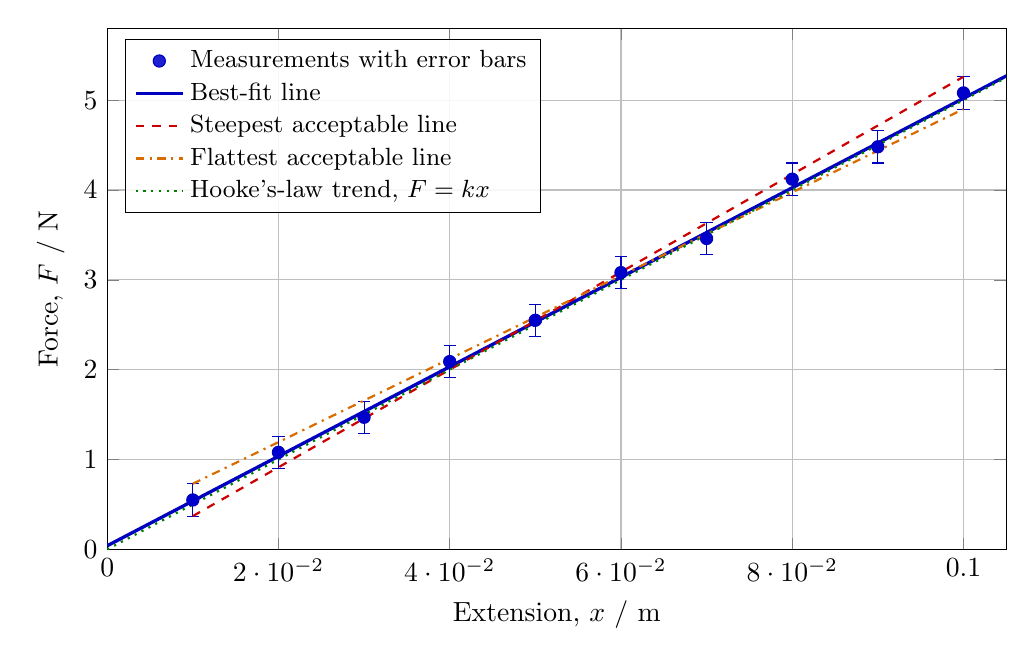
\begin{tikzpicture}
\begin{axis}[
  width=13cm,
  height=8.2cm,
  xlabel={Extension, $x$ / m},
  ylabel={Force, $F$ / N},
  xmin=0, xmax=0.105,
  ymin=0, ymax=5.8,
  xtick={0,0.02,0.04,0.06,0.08,0.10},
  ytick={0,1,2,3,4,5},
  grid=major,
  legend style={
    at={(0.02,0.98)},
    anchor=north west,
    font=\small,
    fill=white,
    fill opacity=0.88,
    text opacity=1
  },
  legend cell align={left}
]
% Representative Hooke's-law measurements with vertical uncertainties.
\addplot+[
  only marks,
  mark=*,
  mark size=2.2pt,
  blue!75!black,
  error bars/.cd,
    y dir=both,
    y explicit
] coordinates {
  (0.010,0.55) +- (0,0.18)
  (0.020,1.08) +- (0,0.18)
  (0.030,1.47) +- (0,0.18)
  (0.040,2.09) +- (0,0.18)
  (0.050,2.55) +- (0,0.18)
  (0.060,3.08) +- (0,0.18)
  (0.070,3.46) +- (0,0.18)
  (0.080,4.12) +- (0,0.18)
  (0.090,4.48) +- (0,0.18)
  (0.100,5.08) +- (0,0.18)
};
\addlegendentry{Measurements with error bars}

% Linear regression: F = kx + c, consistent with Hooke's law.
\addplot[blue!75!black, very thick, domain=0:0.105]
  {49.8*x + 0.04};
\addlegendentry{Best-fit line}

% Limiting acceptable gradients through the first and last error bars.
\addplot[red!80!black, thick, dashed, domain=0.010:0.100]
  {54.333*x - 0.1733};
\addlegendentry{Steepest acceptable line}

\addplot[orange!85!black, thick, dashdotted, domain=0.010:0.100]
  {46.333*x + 0.2667};
\addlegendentry{Flattest acceptable line}

% The ideal theoretical trend F = kx passes through the origin.
\addplot[green!50!black, thick, dotted, domain=0:0.105]
  {50*x};
\addlegendentry{Hooke's-law trend, $F=kx$}
\end{axis}
\end{tikzpicture}
\end{center}
Worst acceptable line / error line (flattest: straight line passing through the highest point in first error bar and the lowest point in the last error bar; steepest: straight line passing through the lowest point in first error bar and the highest point in the last error bar)\\
Gradient (including uncertainties): $m\pm\dfrac{|m_1-m_2|}{2}$\\
Intercept (including uncertainties): $c\pm\dfrac{|c_1-c_2|}{2}$
\subsection{Linearization of graph}
\begin{itemize}
	\item Non-logarithmic approach: transform the relationship into linear relationship via changing the x-axis being graphed against (e.g. $y\propto x^2$) This is learnt in Additional Mathematics, so it should be a revisit.
	\item Logarithmic approach: transform the relationship into linear ones via applying logarithmic functions (Example: $y=ax^b \Rightarrow \log y = b\log x+\log a$; Example 2: $y=ae^{bx} \Rightarrow \ln y=\ln a+bx$)
\end{itemize}
\begin{center}
\begin{tikzpicture}
% Left: original non-linear graph y = 2x^2
\begin{scope}
\draw[->] (0,0) -- (3.4,0) node[below left] {$x$};
\draw[->] (0,0) -- (0,3.2) node[below left] {$y$};
\draw[blue, thick, domain=0:1.15, samples=50] plot (\x,{2*\x*\x});
\node at (1.7,-0.9) {Original: $y=2x^{2}$ (curve)};
\end{scope}
% Arrow
\draw[-{Stealth}, line width=1.2pt] (3.8,1.4) -- (5.0,1.4)
  node[midway, above, align=center, font=\small] {re-plot against\\[-2pt] $x^{2}$};
% Right: linearized graph y vs x^2
\begin{scope}[xshift=7cm]
\draw[->] (0,0) -- (3.4,0) node[below left] {$x^{2}$};
\draw[->] (0,0) -- (0,3.2) node[below left] {$y$};
\draw[red, thick, domain=0:1.32] plot (\x,{2*\x});
\fill (1.0,2.0) circle (1.5pt);
\draw[dashed, gray] (1.0,0) node[below] {$x^{2}_{0}$} -- (1.0,2.0) -- (0,2.0) node[left] {$y_{0}$};
\node at (1.7,-0.9) {Linearized: $y=2x^{2}$, gradient $=2$};
\end{scope}
\end{tikzpicture}
\end{center}
% ===================== Unit A (implicit) =====================
\unnumberedsection{Unit A Space, time and motion}
\section{Kinematics}
Kinematics vs Dynamics: kinematics \emph{describes} motion (displacement, velocity, acceleration) without regard to its cause, while dynamics \emph{explains} motion through forces (Newton's laws).
\subsection{Displacement, distance, speed and velocity}
Displacement 位移: change in position, $\Delta s=s_{\text{final}}-s_{\text{start}}$.\\
Distance 路程: the actual length of the path followed\\
For uniform motion (constant speed):
\begin{itemize}
  \item $v=\dfrac{\Delta s}{\Delta t}$, average speed is total distance divided by total time taken
  \item $s=s_i+vt$
  \item Area in a $v-t$ graph is the displacement
\end{itemize}
\subsection{Uniformly accelerated motion: the equations of kinematics}
For uniformly accelerated motion (constant acceleration):
\begin{itemize}
  \item $\overline{v}=\dfrac{\Delta s}{\Delta t}$
  \item $\displaystyle v=\lim_{\Delta t \to 0}\dfrac{\Delta s}{\Delta t}$
  \item Draw a tangent line to find the instantaneous speed.
  \item $\overline{a}=\dfrac{\Delta v}{\Delta t}$
  \item $\displaystyle a=\lim_{\Delta t \to 0}\dfrac{\Delta v}{\Delta t}$
  \item $v=u+at$, where $u$ is the initial velocity.
  \item $\Delta s=\left(\dfrac{u+v}{2}\right)t=ut+\dfrac{1}{2}at^2$
  \item $s=s_i+ut+\dfrac{1}{2}at^2$
  \item $v^2=u^2+2a\Delta s$
\end{itemize}
Acceleration of freefall: $g=9.8\ \text{m/s}^2$, direction is vertically downwards.\\
Utilize this for questions involving freefall acceleration. (When doing questions, use the negative value.)
\begin{itemize}
\item $s=\dfrac{1}{2}gt^2$
\item $V_f=gt$
\item $v^2=2gh$ (derived from $v^2=u^2+2as$)
\end{itemize}

\subsection{Graphs of motion}
For any motion graph:
\[
  v=\frac{ds}{dt},\qquad a=\frac{dv}{dt}=\frac{d^2s}{dt^2}
\]
and the area under a $v-t$ graph gives displacement, while the area under
an $a-t$ graph gives change in velocity. \\\\Take $x=2\pi t$, where $0\leq x\leq 2\pi$ corresponds to
$0\leq t\leq 1.0\,\mathrm{s}$. If
\[
  s(t)=\sin(2\pi t),
\]
then
\[
  v(t)=\frac{ds}{dt}=2\pi\cos(2\pi t),\qquad
  a(t)=\frac{dv}{dt}=-(2\pi)^2\sin(2\pi t).
\]

\begin{figure}[ht!]
\centering
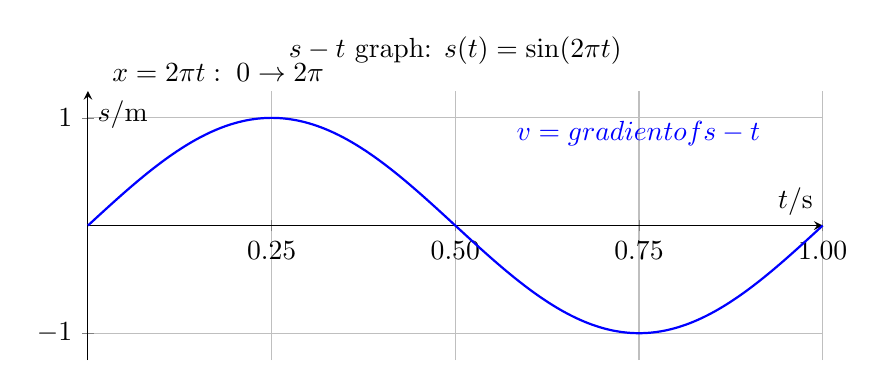
\begin{tikzpicture}
\begin{axis}[
  width=0.9\linewidth,
  height=5cm,
  axis lines=middle,
  xmin=0, xmax=1,
  ymin=-1.25, ymax=1.25,
  xlabel={$t/\mathrm{s}$},
  ylabel={$s/\mathrm{m}$},
  title={$s-t$ graph: $s(t)=\sin(2\pi t)$},
  xtick={0,0.25,0.5,0.75,1},
  xticklabels={$0$,$0.25$,$0.50$,$0.75$,$1.00$},
  ytick={-1,0,1},
  grid=major,
  samples=200,
  domain=0:1,
  clip=false
]
\addplot[blue, thick] {sin(deg(2*pi*x))};
\node[anchor=west, blue] at (axis cs:0.57,0.85) {$v=\text{gradient of }s-t$};
\node[anchor=west] at (axis cs:0.02,1.42) {$x=2\pi t:\;0\to2\pi$};
\end{axis}
\end{tikzpicture}

\vspace{0.4cm}

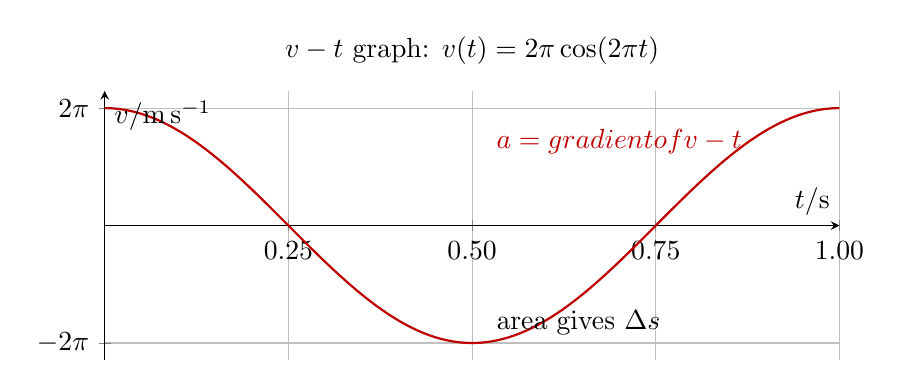
\begin{tikzpicture}
\begin{axis}[
  width=0.9\linewidth,
  height=5cm,
  axis lines=middle,
  xmin=0, xmax=1,
  ymin=-7.2, ymax=7.2,
  xlabel={$t/\mathrm{s}$},
  ylabel={$v/\mathrm{m\,s^{-1}}$},
  title={$v-t$ graph: $v(t)=2\pi\cos(2\pi t)$},
  xtick={0,0.25,0.5,0.75,1},
  xticklabels={$0$,$0.25$,$0.50$,$0.75$,$1.00$},
  ytick={-6.28318,0,6.28318},
  yticklabels={$-2\pi$,$0$,$2\pi$},
  grid=major,
  samples=200,
  domain=0:1,
  clip=false
]
\addplot[red!75!black, thick] {2*pi*cos(deg(2*pi*x))};
\node[anchor=west, red!75!black] at (axis cs:0.52,4.5) {$a=\text{gradient of }v-t$};
\node[anchor=west] at (axis cs:0.52,-5.2) {area gives $\Delta s$};
\end{axis}
\end{tikzpicture}

\vspace{0.4cm}

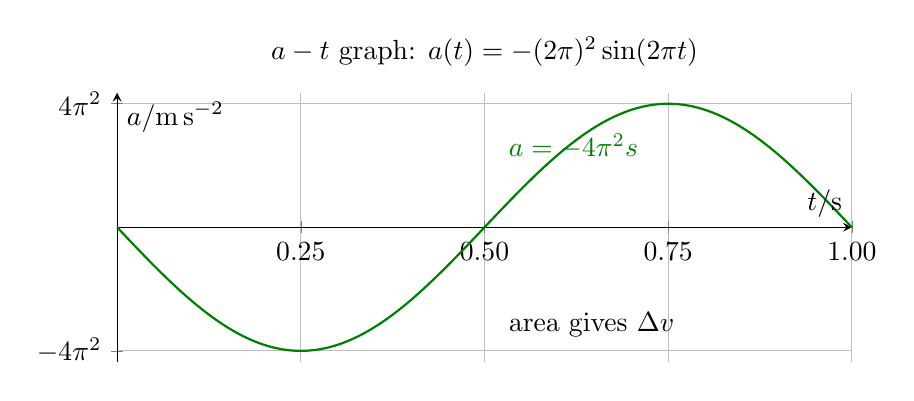
\begin{tikzpicture}
\begin{axis}[
  width=0.9\linewidth,
  height=5cm,
  axis lines=middle,
  xmin=0, xmax=1,
  ymin=-43, ymax=43,
  xlabel={$t/\mathrm{s}$},
  ylabel={$a/\mathrm{m\,s^{-2}}$},
  title={$a-t$ graph: $a(t)=-(2\pi)^2\sin(2\pi t)$},
  xtick={0,0.25,0.5,0.75,1},
  xticklabels={$0$,$0.25$,$0.50$,$0.75$,$1.00$},
  ytick={-39.4784,0,39.4784},
  yticklabels={$-4\pi^2$,$0$,$4\pi^2$},
  grid=major,
  samples=200,
  domain=0:1,
  clip=false
]
\addplot[green!50!black, thick] {-4*pi*pi*sin(deg(2*pi*x))};
\node[anchor=west, green!50!black] at (axis cs:0.52,26) {$a=-4\pi^2s$};
\node[anchor=west] at (axis cs:0.52,-31) {area gives $\Delta v$};
\end{axis}
\end{tikzpicture}
\caption{The $s-t$, $v-t$, and $a-t$ graphs for one cycle of sinusoidal motion.}
\end{figure}
\subsection{Projectile motion}
Types of projectiles:
\begin{itemize}
\item Up and down
\item At an angle to horizontal
\item Horizontal
\end{itemize}
If a projectile is launched at angle $\theta$ and initial speed $u$, then the direction of the velocity are:
\begin{itemize}
  \item $V_x=u\cos\theta$
  \item $V_y=u\sin\theta-gt$
\end{itemize}
The position is determined by position vector $\vec{r}$ that is relative from the origin.
\begin{itemize}
  \item $x=ut\cos\theta$
  \item $y=ut\sin\theta-\dfrac{1}{2}gt^2$
  \item $v_x^2=v_y^2-2gy$
  \item $t=\dfrac{u\sin\theta}{g}$, this is when $v_y=0$.
  \item $y_{\text{max}}=\dfrac{u^2\sin^2\theta}{2g}$, the maximum height
  \item $t=2\dfrac{u\sin\theta}{g}$, this is when the maximum displacement in the $x$-direction occurs.
  \item Maximum displacement in the $x$-direction (\textbf{the range}): $x=\dfrac{u^2\sin 2\theta}{g}$. 
\item We obtain the maximum range with a launch angle of 45$^\circ$.
\end{itemize}
A fluid resistance force is directed against the direction of the velocity. If there is air resistance, it is proportional to the square of the velocity. Thus, when the ball moves fast its deceleration is greater than when it moves slow. (Peak to left of the original one, pre-peak distance > post-peak distance, post-peak gradient > pre-peak gradient)
\begin{itemize}
\item Range decreased
\item Trajectory not parabolic
\item Reduced maximum height
\item Vertical acceleration is no longer constant
\item Horizontal deceleration
\item Speeds reduced
\item Determination of time of flight becomes complex and depends on the initial conditions of the flight
\end{itemize}
$F=kv$ for low speeds and $F=kv^2$ for high speeds. (For resistance)\\
Terminal speed: $v_T=\dfrac{mg}{k}$, where acceleration equals 0.
\section{Forces and Newton's laws}
\subsection{Forces and their direction}
\begin{itemize}
  \item Weight
  \begin{itemize}
    \item $W=mg$
    \item Acts vertically downward
  \end{itemize}
  \item String tension
  \begin{itemize}
    \item The force that arises in any body when it is stretched or compressed, when two forces are applied in opposite directions at the ends of the string 
    \item Taut: under tension
    \item Result of interactions between the molecules in the material, electrical in nature
    \item Usually assume string is massless, tension is same on all points along the string
    \item Direction: along the string
    \begin{center}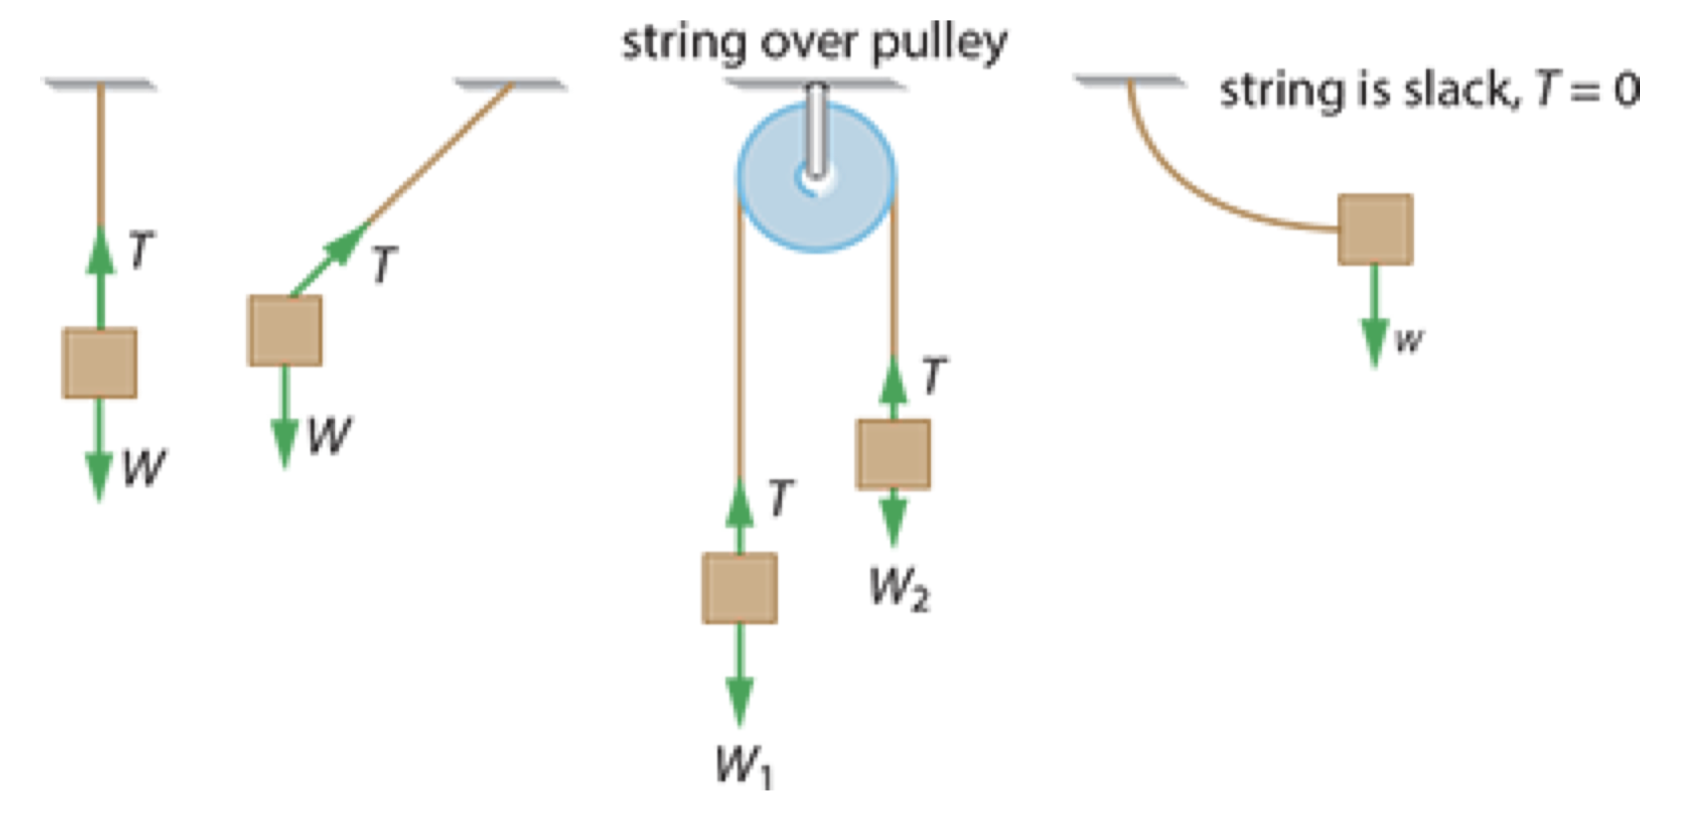
\includegraphics[width=0.5\linewidth]{截圖 2026-05-24 10.59.10.png}\end{center}
  \end{itemize}
  \item Spring tension / Hooke's Law
  \begin{itemize}
    \item Hooke's Law: $F=kx$, where $x$ is the extension
    \item Beyond limit of proportionality: Force no longer varies directly with extension
    \item Elastic limit: The maximum stress a material can withstand and still return completely to its original shape when the load is removed.
    \item Extension on Hooke's Law related content:
    \begin{itemize}
        \item Parallel connection: $F_T=(k_A+k_B)x=k_\text{eff}x$
        \item Series connection: $x_T=x_A+x_B=\dfrac{F}{k_A}+\dfrac{F}{k_B}$; $\dfrac{1}{k_\text{eff}}=\dfrac{1}{k_A}+\dfrac{1}{k_B}$
        \end{itemize}
  \end{itemize}
  \item Normal contact forces
  \begin{itemize}
    \item When a body touches another body
    \item Perpendicular to the surface of the body exerting the force, electrical nature
  \end{itemize}
  \item Drag forces (friction in fluids)
	\begin{itemize}
    \item Opposes the motion of a body through a fluid
    \item For the case of a spherical body of radius $r$ falling through a fluid of density $\rho$ with speed $v$ the drag force is given by Stoke's law:
    \item $F_D=6\pi\eta rv$, where $\eta$ is the viscosity of the fluid (a measure of the forces between layers of the fluid that are moving relative to each other, unit Pa$\times$s)
  \end{itemize}
  \item Buoyant forces (upthrust)
  \begin{itemize}
    \item $F_B=\rho g V_{\text{imm}}$, where $V_\text{imm}$ is the volume of the body that is immersed in the fluid.
    \item Caused by the pressure that the fluid exerts on the body.
    \item 王忠 Let's go: $F_\text{浮}=\rho_\text{液}gV_\text{排}$
  \end{itemize}
  \item Frictional forces
  \begin{itemize}
    \item Generally oppose the motion of a body, electrical nature, parallel to contact surface
    \item Occurs when one body slides over another / has a tendency for motion, has dynamic / static friction
    \begin{center}
	    {\bfseries\small Simple atoms-and-springs model}

    \begin{tikzpicture}[
      atom/.style={circle, draw=blue!55!black, fill=blue!12, thick, minimum size=5mm, inner sep=0pt},
      lower atom/.style={circle, draw=orange!70!black, fill=orange!18, thick, minimum size=5mm, inner sep=0pt},
      spring/.style={decorate, decoration={coil, aspect=0.55, segment length=2.6mm, amplitude=1.05mm}, thick, gray!75!black},
      force/.style={-{Latex[length=3mm]}, very thick},
      label/.style={font=\small, align=center}
    ]
      \draw[fill=blue!5, draw=blue!35] (0,1.55) rectangle (6.8,2.05);
      \draw[fill=orange!8, draw=orange!45] (0,-0.05) rectangle (6.8,0.45);
      \node[label, anchor=west] at (6.95,1.80) {upper};
      \node[label, anchor=west] at (6.95,0.20) {lower};

      \foreach \xb/\xt in {0.7/1.2, 2.2/2.7, 3.7/4.2, 5.2/5.7} {
        \node[atom] at (\xt,1.80) {};
        \node[lower atom] at (\xb,0.20) {};
        \draw[spring] (\xt,1.55) -- (\xb,0.45);
      }

      \draw[force, green!45!black] (0.8,2.40) -- (2.6,2.40);
      \node[label, green!45!black, anchor=south] at (1.7,2.44) {pull};
      \draw[force, red!75!black] (6.3,2.40) -- (4.9,2.40);
      \node[label, red!75!black, anchor=south] at (5.6,2.44) {$f$};
    \end{tikzpicture}

    {\small Atoms are displaced; stretched microscopic bonds act like springs and push back.}

    \vspace{0.2cm}

    {\bfseries\small Asperities model}

    \begin{tikzpicture}[
      force/.style={-{Latex[length=3mm]}, very thick},
      label/.style={font=\small, align=center},
      callout/.style={font=\small\bfseries, align=center, draw=red!70!black, fill=white, rounded corners=1pt, inner sep=2pt},
      pointer/.style={-{Latex[length=2mm]}, thick, red!70!black}
    ]
      \draw[fill=blue!5, draw=blue!45, thick]
        (0,1.55) -- (1.0,1.06) -- (1.85,1.60) -- (3.9,1.02) -- (4.75,1.62) --
        (6.7,1.04) -- (8.0,1.55) -- (8.0,2.1) -- (0,2.1) -- cycle;

      \draw[fill=orange!8, draw=orange!50, thick]
        (0,0.70) -- (1.0,1.06) -- (1.7,0.68) -- (2.5,1.12) -- (3.2,0.66) --
        (3.9,1.02) -- (4.6,0.70) -- (5.3,1.10) -- (6.0,0.64) -- (6.7,1.04) --
        (8.0,0.70) -- (8.0,-0.1) -- (0,-0.1) -- cycle;

      \foreach \x/\y in {1.0/1.06, 3.9/1.02, 6.7/1.04} {
        \draw[red!75!black, line width=1.1pt] (\x-0.10,\y-0.06) -- (\x+0.10,\y+0.10);
        \draw[red!75!black, line width=1.1pt] (\x+0.10,\y-0.06) -- (\x-0.10,\y+0.10);
      }

      \draw[force, blue!70!black] (4.4,2.60) -- (4.4,2.15);
      \node[label, blue!70!black, anchor=west] at (4.55,2.40) {$N$};
      \draw[force, green!45!black] (0.8,2.40) -- (2.6,2.40);
      \node[label, green!45!black, anchor=south] at (1.7,2.44) {pull};
      \draw[force, red!75!black] (7.8,1.80) -- (6.4,1.80);
      \node[label, red!75!black, anchor=south] at (7.1,1.84) {$f$};
      \node[callout] (junctions) at (3.9,-0.80) {microscopic\\junctions};
      \draw[pointer] (junctions.north west) -- (1.0,1.06);
      \draw[pointer] (junctions.north east) -- (6.7,1.04);
    \end{tikzpicture}

    {\small Real surfaces touch at asperities; junctions must shear or break before sliding occurs.}
  \end{center}
    \item Friction Laws:
    \begin{enumerate}
      \item Area of contact does not affect the frictional force.
      \item The force of dynamic friction is $f_d=\mu_dR$, where $R$ is the normal force and $\mu_d$ is the coefficient of dynamic friction.
      \item The force of dynamic friction does not depend on the speed of sliding.
      \item The MAXimum force of static friction is $f_s=\mu_sR$, where $\mu_s$ is the coefficient of static friction and $\mu_s>\mu_d$
      \item ($\mu_sR$ does not give the force of static friction, but only the MAXimum)
      \item $0\leq F_s\leq F_{s,\max}$; $F_d<F_{s,\max}$; $F_d=k$
	    \end{enumerate}
\begin{center}
    \begin{tikzpicture}[
      axis/.style={-{Latex[length=3mm]}, thick},
      curve/.style={very thick, blue!70!black},
      drop/.style={very thick, blue!70!black, dashed},
      guide/.style={gray!70, dashed},
      label/.style={font=\small}
    ]
      \draw[axis] (0,0) -- (7.2,0) node[below] {$F$};
      \draw[axis] (0,0) -- (0,4.6) node[left] {$f$};

      \draw[guide] (0,3.3) -- (3.3,3.3);
      \draw[guide] (0,2.1) -- (7.0,2.1);
      \draw[guide] (3.3,0) -- (3.3,3.3);

      \draw[curve] (0,0) -- (3.3,3.3);
      \draw[drop] (3.3,3.3) -- (3.3,2.1);
      \draw[curve] (3.3,2.1) -- (7.0,2.1);

      \node[label, left] at (0,3.3) {$f_{s,\max}=\mu_sR$};
      \node[label, left] at (0,2.1) {$f_d=\mu_dR$};
      \node[label, below] at (3.3,0) {$F=f_{s,\max}$};
      \node[label, rotate=45, above] at (1.55,1.75) {$f=F$};
      \node[label, above] at (5.25,2.1) {$f=f_d$};
      \node[label, below] at (1.6,-0.25) {static};
      \node[label, below] at (5.25,-0.25) {dynamic};
    \end{tikzpicture}
  \end{center}

	\item Explaining friction:
	\begin{itemize}
	    \item At the atomic level when two surfaces come into contact, small peaks on one surface cold weld with small peaks on the other surface.
	    \item Applying the initial sideways force, all of the cold welds oppose the motion.
	    \item If the force is sufficiently large, the cold welds break, and new peaks contact each other and cold weld.
	    \item If the surfaces remain in relative sliding motion, fewer welds have a chance to form.
	    \item The coefficient of friction is then defined as $\mu=\dfrac{f}{R}$
	    \end{itemize}
\end{itemize}
  \end{itemize}
Free-body force diagrams: diagram showing the magnitude and direction of all the forces acting on a chosen body. The length of the arrow representing a given force is proportional to the magnitude of the force. Very useful when trying to solve complex questions especially involving $F=ma$ (will be covered very soon)\\\\
Equilibrium: $\displaystyle \sum F=0$, the resultant / net force is zero.

\subsection{Newton's laws of motion}
\begin{enumerate}
  \item Law of inertia: When the net force on a body is zero, the body will move with constant velocity (which may be zero); in other words, it will move on a straight line with constant speed (which may be zero). An object will remain at erst or move at constant velocity unless it is acted on by a resultant force.
  \item The net force on a body of constant mass is proportional to that body's acceleration and is in the same direction as the acceleration. The resultant force on one object is equal to the rate of change of momentum. \[\vec{F}=m\vec{a}; F=\dfrac{\Delta p}{t}=\dfrac{mv-mu}{t}\]
  \item If body X exerts a force on body Y, then body Y will exert an equal and opposite force on body X. When two bodies interact, they exert on each other the forces of the same type, equal in magnitude but opposite in direction simultaneously.
\end{enumerate}
Solving equilibrium problems involving various forces by spliting the forces into $F_x$ and $F_y$ components.\\
How to solve an $F=ma$ problem:
\begin{enumerate}
  \item Make a diagram and choose the direction that you will take as positive. 
  \item Make a free-body diagram. (\textbf{Very important!})
  \item Find the net force by looking at the free-body diagram.
  \item Set the net force equal to ma.
  \item Solve for what is unknown.
\end{enumerate}
Questions involving inclined plane: (assumed with friction)
\begin{center}
  \begin{tikzpicture}[
    force/.style={-{Latex[length=3mm]}, very thick},
    component/.style={-{Latex[length=3mm]}, thick, dashed},
    plane/.style={thick},
    block/.style={draw=orange!70!black, fill=orange!15, thick},
    label/.style={font=\small}
  ]
    \coordinate (A) at (0,0);
    \coordinate (B) at (8,0);
    \coordinate (C) at (8,3.8);
    \coordinate (P) at (4.1,2.0);
    \coordinate (O) at (3.94,2.34);

    \fill[gray!15] (A) -- (B) -- (C) -- cycle;
    \draw[plane] (A) -- (B) -- (C) -- cycle;
    \draw[plane] (A) -- (C);

    \draw (0.75,0) arc[start angle=0,end angle=25.4,radius=0.75];
    \node[label] at (1.05,0.22) {$\theta$};

    \begin{scope}[shift={(P)}, rotate=25.4]
      \draw[block] (-0.65,0) rectangle (0.65,0.75);
    \end{scope}

    \fill (O) circle (1.5pt);

    \draw[force, red!75!black] (O) -- ++(0,-2.0)
      node[below right, right=3pt] {$mg$};
    \draw[force, blue!70!black] (O) -- ++(115.4:1.6) node[above left] {$R$};
    \draw[force, green!45!black] (O) -- ++(25.4:1.8) node[right] {$f$};

    \draw[component, purple!75!black] (O) -- ++(205.4:1.7)
      node[pos=0.45, above left=2pt] {$mg\sin\theta$};
    \draw[component, purple!75!black] (O) -- ++(-64.6:1.35)
      node[pos=0.45, right=4pt] {$mg\cos\theta$};
  \end{tikzpicture}
\end{center}
where $R=mg\cos\theta$, the normal force; $f=mg\sin\theta$, the frictional force.
$\mu_s=\tan \theta_\text{max}$, where $\theta_\text{max}$ is the largest angle of the inclined plane at which we can have equilibrium.
$a=g\sin\theta$ (if plane turns frictionless)
\subsection{Circular motion}
Circular motion requires the presence of a force directed towards the center of the circle.
\[v=\dfrac{2\pi r}{T}=r\omega=2\pi rf\]
where $T=\dfrac{2\pi r}{v}=\dfrac{2\pi}{\omega}$ is the period / time taken for one complete revolution.\\
\[\text{Angular speed} = \omega =\dfrac{\text{angle swept}}{\text{time taken}}=\dfrac{\Delta\theta}{\Delta t}\]
For a complete revolution, $\omega=\dfrac{2\pi}{T}=2\pi f$.\\
Frequency, the number of complete revolutions in one second: $f=\dfrac{1}{T}$.\\
Centripetal acceleration, normal to the circle and directed toward the center of the circle:
\[a_c=v\omega=\dfrac{v^2}{r}=\omega^2 r=\dfrac{4\pi ^2 r}{T^2}=4\pi^2rf^2\]
The centripetal force is directed towards the center of the circle (the direction of the net force). \\
A car will skid outward (i.e., will cover a circle of larger radius) if the friction force is not large enough.
\begin{center}
  \begin{tikzpicture}[
    force/.style={-{Latex[length=3mm]}, very thick},
    velocity/.style={-{Latex[length=3mm]}, very thick, blue!70!black},
    acceleration/.style={-{Latex[length=3mm]}, very thick, red!75!black},
    path/.style={thick, dashed, gray!70!black},
    skid/.style={-{Latex[length=3mm]}, very thick, red!75!black},
    car/.style={draw=black, fill=gray!18, thick},
    road/.style={very thick},
    label/.style={font=\small}
  ]
    \begin{scope}
      \coordinate (C) at (0,0);
      \coordinate (P) at (35:1.6);

      \draw[path] (C) circle (1.6);
      \fill (C) circle (1.3pt);
      \draw[path] (C) -- (P) node[midway, below right, label] {$r$};

      \begin{scope}[shift={(P)}, rotate=125]
        \draw[car] (-0.38,-0.18) rectangle (0.38,0.18);
      \end{scope}

      \draw[velocity] (P) -- ++(125:1.0) node[above left, label] {$v$};
      \draw[acceleration] (P) -- ++(215:0.95) node[left, label] {$a_c$};
      \node[label] at (0,-2.25) {top view};
    \end{scope}

    \begin{scope}[shift={(5.2,0)}]
      \draw[road] (-1.8,-0.55) -- (1.8,-0.55);
      \draw[car] (-0.75,-0.55) rectangle (0.75,0.05);
      \fill (-0.48,-0.58) circle (0.08);
      \fill (0.48,-0.58) circle (0.08);
      \coordinate (Q) at (0,-0.15);

      \draw[force, red!75!black] (Q) -- ++(0,-1.05) node[below, label] {$mg$};
      \draw[force, blue!70!black] (Q) -- ++(0,1.2) node[above, label] {$R$};
      \draw[force, green!45!black] (Q) -- ++(-1.35,0) node[left, label] {$f$};
      \node[label] at (0,-2.25) {side view};
    \end{scope}

    \begin{scope}[shift={(10.7,0)}]
      \coordinate (C2) at (0,0);
      \coordinate (P2) at (25:1.25);

      \draw[path] (C2) circle (1.25);
      \draw[path, red!50!black] (C2) circle (1.9);
      \fill (C2) circle (1.3pt);
      \draw[path] (C2) -- (P2) node[midway, below right, label] {$r$};

      \begin{scope}[shift={(P2)}, rotate=115]
        \draw[car] (-0.36,-0.17) rectangle (0.36,0.17);
      \end{scope}

      \draw[velocity] (P2) -- ++(115:0.9) node[above left, label] {$v$};
      \draw[skid] (P2) .. controls (70:2.15) and (90:1.95) .. (105:1.9)
        node[above, label] {larger radius};
      \node[label] at (0,-2.25) {speed too high};
    \end{scope}
  \end{tikzpicture}
\end{center}
Question: A particle is tied to a string and moves with constant speed in a horizontal circle. The string is tied to the ceiling. Draw the forces on the particle.\\
The common mistake here is to put a horizontal force pointing toward the center and call it the centripetal force. But in fact, it already exists (the horizontal component of the tension).
\begin{center}
  \begin{tikzpicture}[
    force/.style={-{Latex[length=3mm]}, very thick},
    component/.style={-{Latex[length=3mm]}, thick, dashed},
    string/.style={very thick},
    normal/.style={thick, dashed, gray!70!black},
    path/.style={thick, dashed, gray!70!black},
    label/.style={font=\small}
  ]
    \begin{scope}
      \coordinate (P) at (0,1.8);
      \coordinate (M) at (1.5,0);
      \coordinate (C) at (0,0);

      \draw[thick] (-1.2,1.8) -- (1.2,1.8);
      \fill (P) circle (1.4pt);
      \draw[normal] (P) -- (C);
      \draw[string] (P) -- (M);
      \draw[path] (C) ellipse (1.5 and 0.35);
      \draw[path] (C) -- (M) node[midway, below, label] {$r$};
      \fill[blue!20, draw=blue!70!black, thick] (M) circle (0.16);
      \draw[force, blue!70!black] (M) -- ++(-0.75,0.9)
        node[midway, above right, label] {$T$};
      \draw[force, red!75!black] (M) -- ++(0,-0.9)
        node[right, label] {$mg$};

      \draw (0,1.35) arc[start angle=-90,end angle=-50,radius=0.45];
      \node[label] at (0.28,1.18) {$\theta$};
    \end{scope}

    \begin{scope}[shift={(5.0,0.15)}]
      \coordinate (Q) at (0,0);

      \fill[blue!20, draw=blue!70!black, thick] (Q) circle (0.16);
      \draw[force, blue!70!black] (Q) -- ++(130:2.0) node[above left, label] {$T$};
      \draw[force, red!75!black] (Q) -- ++(0,-1.65) node[below, label] {$mg$};

      \draw[component, blue!55!black] (Q) -- ++(0,1.3)
        node[above, label] {$T\cos\theta$};
      \draw[component, blue!55!black] (Q) -- ++(-1.35,0)
        node[left, label] {$T\sin\theta$};
    \end{scope}
  \end{tikzpicture}
\end{center}
The steps to solve problems on circular motion:
\begin{enumerate}
    \item Analyze the state of motion of the studied object (if it is in a state of uniform circular motion).
    \item Determine the center and the radius of the circle.
    \item Analyze the forces, determine the origin of centripetal force, and
calculate the resultant force in the direction to the center of the
circle.
	\item The resultant force provides the centripetal force of the circular
motion.
\end{enumerate}
\section{Work, energy and power}
\subsection{Work}
Work done by a constant force for motion in straight line:
\[W=Fs\cos\theta=F\times d\]
The distance travelled by the body is s. \\The force makes an angle $\theta$ with the displacement. \\Definition: The work done by a force is the product of the force in the direction of the displacement times the distance travelled.
\begin{center}
  \begin{tikzpicture}[
    force/.style={-{Latex[length=3mm]}, very thick},
    displacement/.style={-{Latex[length=3mm]}, thick},
    block/.style={draw=black, fill=gray!18, thick},
    label/.style={font=\small}
  ]
    \coordinate (A) at (0,0);
    \coordinate (B) at (6,0);
    \coordinate (P) at (1.4,0.55);

    \draw[thick] (-0.4,0) -- (6.8,0);
    \draw[block] (0.7,0) rectangle (2.1,0.9);

    \draw[displacement, blue!70!black] (1.4,-0.45) -- (5.6,-0.45)
      node[midway, below, label] {$s$};
    \draw[force, red!75!black] (P) -- ++(32:2.3)
      node[above right, label] {$F$};
    \draw[gray!70!black, thick] (P) -- ++(2.0,0);
    \draw (P) ++(0.6,0) arc[start angle=0,end angle=32,radius=0.6];
    \node[label] at (2.23,0.78) {$\theta$};
  \end{tikzpicture}
\end{center}
(向量点积：想起我了没? 晚了！怒气冲天ing)\\
Value could be negative. Unit is J / N$\cdot$m.\\\\
Work done by varying force: Area under a curve / integral\\\\
Work done in circular motion: work done by centripetal force is 0. (the path followed instantaneously and the direction of the force forms an angle of 90 degrees, and $\cos 90^\circ=0$)
\[Fs=\dfrac{1}{2}mv^2-\dfrac{1}{2}mu^2\]
where $Fs$ is the work done by the particle.
\[E_k=\dfrac{1}{2}mv^2\]
\[\text{Work-kinetic energy relation: }W_\text{net}=\Delta E_k\]
The work done has resulted in a transfer of energy that has changed the kinetic energy of the particle.\\\\
Work done by gravity: 0 if the displacement is horizontal. ($W=mgs\cos 90^\circ=0$)\\
In other words: When a body is displaced such that its final position is at the same vertical height as the original position, the work done by the weight is zero.
\[\text{Work done by weight}=E_\text{p}=mg\Delta h\]
(Definition of gravitational potential energy: the work done by the moving force in placing a body a height $h$ above the surface of the earth)\\
This implies that a body on the surface has zero potential energy.\\
This formula is approximate and may only be used if the height h is very small compared to the radius of the earth.\\
Positive if object is lowered, negative if object raised.\\\\
The work to extend a spring from its natural length by an amount x is
\[W=\text{Elastic potential energy, } E_H=\dfrac{1}{2}kx^2=\dfrac{1}{2}k(x_2^2-x_1^2) \text{ (if two values are present)}\]
where $x$ is the extension and $k$ is the spring constant.
\subsection{Conservation of energy}
Law of conservation of total mechanical energy, $E_T=E_k+E_p(+E_H)=\dfrac{1}{2}mv^2+mg\Delta h\left(+\dfrac{1}{2}kx^2\right)$ only happens when friction and resistance forces are absent and no other forces act on the system from outside the system. In other words, this only happens in an isolated system.\\
If there are interactions between the system and its surroundings, the total mechanical energy may change. These interactions mainly involve work done $W_\text{ext}$ by the surroundings and/or the transfer of thermal energy (heat), $Q$, to or from the surroundings. In this case:
\[\Delta E_T=W_\text{ext} + Q\]
\subsection{Power and efficiency}
Power is the rate at which work is being performed or the rate at which energy is being transferred.
\[P=\dfrac{\Delta W}{\Delta t}=Fv\]
where $F$ is a constant force acting on the body and $v$ is the instantaneous speed of the body. This is the power produced in making the body move at speed $v$.
\[\text{Average power developed}=\overline{F}\times\dfrac{v+u}{2}\]
Efficiency:
\[\eta=\dfrac{\text{Useful energy / power out}}{\text{Actual power / energy in}}\]
\subsection{Energy transfers}
The law of conservation of energy states that energy cannot be created or destroyed: it can only be transferred from one form to another.
\section{Linear momentum}
\subsection{Newton's second law in terms of momentum}
Linear momentum is defined to be the product of the mass of a body and its velocity: \(\vec{p}=m\vec{v}\).\\
Therefore, Newton's second law can be expressed as:
$$\begin{aligned}\vec{F_\text{net}}&=\dfrac{\Delta \vec{p}}{\Delta t}\\&=\dfrac{\vec{p_F}-\vec{p_I}}{\Delta t}\\&=\dfrac{m\vec{v_F}-m\vec{v_I}}{\Delta t}\\&=m\dfrac{\Delta \vec{v}}{\Delta t}\\&=m\vec{a}\end{aligned}$$
\subsection{Impulse and force-time graphs}
\[\vec{J}=\Delta \vec{p}=\vec{F_\text{net}}\Delta t\]
In other words, impulse is the area under the curve in a graph of force against time.
\subsection{Conservation of momentum}
Conservation of momentum: when the net force on a system is zero the momentum does not change and it is conserved. The total momentum of a closed system of colliding objects remains constant in any direction iff no external forces act on the system.\\\\
Consider a ball that you drop from rest from a certain height. As the ball falls, its speed and momentum increase so the momentum of the ball does not stay the same. This is to be expected—there is an external force on the ball, namely its weight. So the momentum of the system that consists of just the falling ball is not conserved. If we include the earth as part of the system, then there are no external forces anymore and the total momentum will be conserved. 
\begin{center}
\begin{tikzpicture}[
  scale=0.9,
  force/.style={-{Latex[length=4mm]}, very thick, red!70!black},
  label/.style={font=\small\bfseries, align=center}
]
  % First diagram: External force
  \begin{scope}[xshift=0cm]
    % Earth
    \fill[blue!30!green] (2, 0) circle (0.8);
    \draw[thick, blue!40!black] (2, 0) circle (0.8);
    \node[label, below] at (2, -1.2) {Earth};
    
    % Ball
    \fill[red] (2, 3) circle (0.5);
    \draw[thick, red!70!black] (2, 3) circle (0.5);
    
    % Dashed ellipse around ball only
    \draw[dashed, orange, line width=2pt] (2, 3) ellipse (1.2 and 0.8);
    
    % Force arrow
    \draw[force] (2, 2.4) -- (2, 1);
    \node[label, red!70!black, right] at (2.3, 1.7) {external force};
  \end{scope}
  
  % Second diagram: Internal force
  \begin{scope}[xshift=6cm]
    % Dashed ellipse containing all elements
    \draw[dashed, orange, line width=2pt] (2, 1.5) ellipse (1.8 and 2.5);
    
    % Earth
    \fill[blue!30!green] (2, 0) circle (0.8);
    \draw[thick, blue!40!black] (2, 0) circle (0.8);
    \node[label, below] at (2, -1.2) {Earth};
    
    % Ball
    \fill[red] (2, 3) circle (0.5);
    \draw[thick, red!70!black] (2, 3) circle (0.5);
    
    % Force arrow
    \draw[force] (2, 2.4) -- (2, 1);
    \node[label, red!70!black, right] at (2.3, 1.7) {internal force};
  \end{scope}
\end{tikzpicture}
\end{center}
\subsubsection*{Extension: rocket equation 火箭方程}
The rocket moves with speed $v$. The engine is turned on, and gases leave the rocket with speed $u$ relative to the rocket. The initial mass of the rocket including the fuel is $M$. After a short time $\delta t$ the rocket has ejected fuel of mass $\delta m$. The mass of the rocket is, therefore, reduced to $M-\delta m$ and its speed increased to $v+\delta v$.
\begin{center}
\resizebox{0.8\textwidth}{!}{%
\begin{tikzpicture}
\draw [ fill={rgb,255:red,71; green,93; blue,255}, fill opacity=1] (4.375,13.5) rectangle (10.75,11.25);
\node[label, left] at (4, 12.375) {$M$};
\draw [ fill={rgb,255:red,233; green,44; blue,1}, fill opacity=1] (5.375,12.375) circle (0.875cm);
\draw [ fill={rgb,255:red,0; green,92; blue,255}, fill opacity=1] (6,10.625) rectangle (12.375,8.375);
\draw [ fill={rgb,255:red,233; green,44; blue,1}, fill opacity=1] (3.875,9.5) circle (0.875cm);
\draw [-{Stealth[scale=1.5]}, ] (11.25,12.375) -- (12.75,12.375);
\node[label, right] at (13,12.375) {$v$}; 
\draw [ fill={rgb,255:red,255; green,255; blue,255}, fill opacity=1] (7,9.5) circle (0.875cm);
\draw [-{Stealth[scale=1.5]}, ] (12.625,9.5) -- (15.375,9.5);
\node[label, above] at (14,9.75) {$v+\delta v$};
\draw [-{Stealth[scale=1.5]}, ] (2.625,9.5) -- (-0.125,9.5);
\node[label, below] at (9,8.2) {$M-\delta m$};
\node[label, below] at (1.5,9.5) {$\delta m$};
\node[label, above] at (1.5,9.6) {$u-(v+\delta v)$};
\end{tikzpicture}
}%

\end{center}
Applying the law of conservation of momentum gives:
$$
\begin{aligned}
Mv&=(M-\delta m)(v+\delta v)-\delta m(\underbrace{u-v-\delta v}_{\text{speed relative to the ground}})\\
Mv&=Mv+M\delta v-v\delta m-\delta m\delta v-u\delta m+v\delta m+\delta m\delta v\\
M\delta v&=u\delta m\\
\delta v&=\dfrac{\delta m}{M}u\\
\lim_{\delta t\to 0}\dfrac{\delta v}{\delta t}&=\dfrac{\delta m}{\delta t}\dfrac{u}{M}\Rightarrow \boxed{M\dfrac{dv}{dt}=u\dfrac{dm}{dt}}
\end{aligned}$$
\subsection{Kinetic energy and momentum}
We observe that whereas momentum is conserved in all cases, kinetic energy is not.\\
When kinetic energy is conserved, the collision is said to be an elastic collision. Relative speed of approach is equal to the relative speed of separation in elastic collision.
\[\left\{
\begin{aligned}
\dfrac{1}{2}m_au_a^2+\dfrac{1}{2}m_bu_b^2&=\dfrac{1}{2}m_av_a^2+\dfrac{1}{2}m_bv_b^2;\\
u_a-u_b&=v_b-v_a;\\
\end{aligned}\right. \]
When kinetic energy is not conserved / lost (transformed into e.g., thermal / deformation / sound energy), the collision is said to be an inelastic collision.
\[\dfrac{1}{2}m_au_a^2+\dfrac{1}{2}m_bu_b^2>\dfrac{1}{2}m_av_a^2+\dfrac{1}{2}m_bv_b^2;\]
(When the bodies stick together after a collision, the collision is said to be totally inelastic and the maximum possible $E_k$ is lost.)\\
Kinetic energy could be calculated as:
\[E_k=\dfrac{1}{2}mv^2=\dfrac{m^2v^2}{2m}=\dfrac{p^2}{2m}\]
\subsection{Two-dimensional collisions}
\begin{center}
\resizebox{0.7\textwidth}{!}{
\begin{circuitikz}
% Changed 18.2pt to standard 17.28pt to stop the font substitution warnings
\tikzstyle{every node}=[font=\fontsize{17.28pt}{22pt}\selectfont]

\draw [-{Stealth[scale=1.5]}, dashed] (2.625,12.5) -- (6.875,12.5);
\draw [ fill={rgb,255:red,255; green,0; blue,0}, fill opacity=1] (3.25,13.25) circle (0.5cm);
\draw [ fill={rgb,255:red,0; green,14; blue,255}, fill opacity=1] (5.875,11.875) circle (0.5cm);
\draw [-{Stealth[scale=1.5]}, ] (11.25,8.875) -- (11.25,16.625);
\draw [-{Stealth[scale=1.5]}, ] (9.125,12.5) -- (19.75,12.5);
\draw [-{Stealth[scale=1.5]}, dashed] (11.25,12.5) -- (17.375,16.5);
\draw [-{Stealth[scale=1.5]}, dashed] (11.25,12.5) -- (18.5,10.625);
\draw [ fill={rgb,255:red,255; green,0; blue,0}, fill opacity=1] (15.25,15.25) circle (0.5cm);
\draw [ fill={rgb,255:red,62; green,18; blue,255}, fill opacity=1] (16,11.25) circle (0.5cm);
\draw [-{Stealth[scale=1.5]}, ] (15.5,10.5) -- (16.5,10.25);

% Simplified node syntax to ensure clean math-mode parsing
\node[below] at (16,10) {$v$};
\node[below] at (4.5,11) {Before};
\node[below] at (10,12) {After};
\node[below] at (14,12.5) {$\theta$};

\end{circuitikz}
}
\end{center}
Key idea:
\[\sum p_{x_\text{before}}=\sum p_{x_\text{after}}\]
\[\sum p_{y_\text{before}}=\sum p_{y_\text{after}}\]
\section{Rigid body mechanics}
\subsection{Kinematics of rotational motion}
Use radians at all times!\\
Consider a particle that rotates around a circle about an axis through the center. The angular position $\theta$ of
the particle is determined by an angle (defined relative to some arbitrary reference line).\\
The angular displacement is the change in angular position by sweeping an angle of $\Delta\theta$.\\
The average angular velocity is defined as
\[\overline{\omega}=\dfrac{\Delta \theta}{\Delta t}\]
The instantaneous angular velocity is defined as
\[\omega=\lim_{\Delta t\to 0}\dfrac{\Delta \theta}{\Delta t}\]
The average angular acceleration is defined as
\[\overline{\alpha}=\dfrac{\Delta\omega}{\Delta t}\]
The instantaneous angular acceleration is defined as
\[\alpha=\lim_{\Delta t\to 0}\dfrac{\Delta\omega}{\Delta t}\]
Correspondence between linear and angular quantities:
\begin{center}
  \renewcommand{\arraystretch}{1.6}
  \begin{tabularx}{\textwidth}{@{}|Y |Y |@{}}
    \toprule
    Linear quantity & Angular quantity \\
    \midrule
    Position $s$ & Angle $\theta$ \\\hline
    Linear velocity $v$ & Angular velocity $\omega$ \\\hline
    Acceleration $a$ & Angular acceleration $\alpha$ \\\hline
    $\Delta s=ut+\dfrac{1}{2}at^2$ & $\Delta \theta=\omega_1t+\dfrac{1}{2}\alpha t^2$\\\hline
    $\Delta s=\dfrac{u+v}{2}t$ & $\Delta \theta=\dfrac{\omega_1+\omega_2}{2}t$\\\hline
    $v=u+at$ & $\omega=\omega_1+\alpha t$\\\hline
    $v^2=u^2+2a\Delta s$ & $\omega^2=\omega_1^2+2\alpha\Delta\theta$\\
    \bottomrule
  \end{tabularx}
\end{center}
Equations relating linear and angular quantities:
\[v=\omega r;\ a=\alpha r\]
Note that this linear acceleration is the rate of change of speed and is not the centripetal acceleration of circular motion.
\subsection{Rotational equilibrium and Newton's second law}
Torque has to do with the ability of a force to produce rotation.\\
Defined as the product of the force times the perpendicular distance between the line of action of the force and the axis:
\[\tau =Fd=Fr\sin\theta\]
where $\theta$ is angle between the force and the vector from the axis to the point where the force is applied.\\
Notice that if the force is directed through the axis, the torque is zero. The force cannot produce a rotation in this case.\\\\
Translational equilibrium: net force of the body is zero. The center of mass of the body remains at rest or moves in a straight line at constant speed.\\
Rotational equilibrium: net torque of the body is zero.\\
Solve equilibrium problems:
\begin{enumerate}
  \item Satisfying translational equilibrium: forces acting downward must equal to the normal force.
  \item Torque for counterclockwise and clockwise direction are equal to each other. 
  \item You may take torques about any axis, not just the actual axis of rotation.
\end{enumerate}
Moment of inertia:
\[I=\sum m_ir_i^2\]
where $m_i$ are the mass of the "bits" that constitutes the body, and $r_i$ are the distance between the bits and the axis (free to rotate about for this rigid body)\\
The moment of inertia depends on the axis we choose. The same body will have different moments of inertia for different axes of rotation.
\[\text{The moment of inertia in rotational motion}\Leftrightarrow\text{Mass in linear motion}\]
\[\text{Torque in rotational motion}\Leftrightarrow\text{Force in linear motion}\]
Some special cases:
\begin{center}
  \begin{tabular}{|c|c|}\hline
    Shape & Formula of moment of inertia \\\hline
    Ring & $I=MR^2$ \\\hline
    Disk / Cylinder & $I=\dfrac{1}{2}MR^2$ \\\hline
    Sphere & $I=\dfrac{2}{5}MR^2$ \\\hline
    Rod & $I=\dfrac{1}{12}ML^2$ \\\hline 
  \end{tabular}
\end{center}
$^*:$ $M=\displaystyle \sum m_i$, the total mass; $R$, radius; $L$, the length (of the rod)\\\\
The kinetic energy of rotational motion:
\[E_k=\sum \dfrac{1}{2}m_iv_i^2=\dfrac{1}{2}\left(\sum m_ir_i^2\right)\omega^2=\dfrac{1}{2}I\omega^2\]
\subsubsection*{Rolling (without slipping)}
\begin{itemize}
  \item Rotates about its axis: All points on the wheel have the same angular velocity and linear speed.
  \item Sliding with velocity $u$ along a horizontal floor: every point on the wheel has a velocity $u$.
  \item Rotates as it moves forward: Every point on the circumference of the wheel now has two motions. The top point has linear velocity of $v=u+\omega R$ and the bottom point has linear velocity of $v=u-\omega R$ (point of contact has zero velocity).
\end{itemize}
In the case of rolling without slipping, $u=\dfrac{2\pi R}{T}=\omega R$, where $R$ is the distance from the center of mass to the point of contact with the ground.
\\If the force is applied
\begin{itemize}
  \item through the center of mass, the ball will slide but will not rotate (there is no torque to cause rotation)
  \item anywhere else, it will cause sliding as well as rotation.
\end{itemize}
Kinetic energy of a body that rolls without slipping:
\[E_k=\underbrace{\left(E_{k_1}=\dfrac{1}{2}Mv^2\right)}_\text{translational motion of the center of mass}+\underbrace{\left(E_{k_2}=\dfrac{1}{2}I\omega^2\right)}_\text{rotational motion}\]
where $v$ is the speed of the center of mass.\\
Total mechanical energy:
\[E_T=\underbrace{\dfrac{1}{2}I\omega^2}_\text{$E_k$ of rotational motion}+\underbrace{\dfrac{1}{2}Mv^2}_\text{$E_k$ of translational motion}+\underbrace{Mgh}_\text{$E_p$ of the body}\]
In the absence of resistance forces the total energy is conserved.\\
In the case of rolling without slipping, $v=\omega R$, $a=\alpha R$.\\\\
Newton's second law applied to the center of the body:
\[F_\text{net}=Ma\Leftrightarrow\tau_\text{net}=I\alpha\]
Apply these two formulas to the question and find a solution accordingly.\\
Linear acceleration of an object rolling without slipping down an inclined plane:
\begin{center}
  \begin{tikzpicture}[
    force/.style={-{Latex[length=3mm]}, very thick},
    component/.style={-{Latex[length=3mm]}, thick, dashed},
    plane/.style={thick},
    block/.style={draw=orange!70!black, fill=orange!15, thick},
    label/.style={font=\small}
  ]
    \coordinate (A) at (0,0);
    \coordinate (B) at (8,0);
    \coordinate (C) at (8,3.8);
    \coordinate (P) at (4.1,2.0);
    \coordinate (O) at (3.94,2.34);

    \fill[gray!15] (A) -- (B) -- (C) -- cycle;
    \draw[plane] (A) -- (B) -- (C) -- cycle;
    \draw[plane] (A) -- (C);

    \draw (0.75,0) arc[start angle=0,end angle=25.4,radius=0.75];
    \node[label] at (1.05,0.22) {$\theta$};

\draw [ fill={rgb,255:red,255; green,200; blue,0}, fill opacity=0.9] (3.9 ,2.4) circle (0.5cm);
    \fill (O) circle (1.5pt);

    \draw[force, red!75!black] (O) -- ++(0,-2.0)
      node[below right, right=3pt] {$mg$};
    \draw[force, blue!70!black] (O) -- ++(115.4:1.6) node[above left] {$N$};
    \draw[force, green!45!black] (O) -- ++(25.4:1.8) node[right] {$f$};
\node[label, right] at (3.9,1.5) {$\theta$};
    \draw[component, purple!75!black] (O) -- ++(205.4:1.7)
      node[pos=0.45, above left=2pt] {$mg\sin\theta$};
    \draw[component, purple!75!black] (O) -- ++(-64.6:1.35)
      node[pos=0.45, right=4pt] {$mg\cos\theta$};
  \end{tikzpicture}
\end{center}
For sphere, $a=\dfrac{5}{7}g\sin\theta$. For other objects, follow the formula $a=\dfrac{g\sin\theta}{1+\dfrac{I}{MR^2}}$.\\
For sphere, $v^2=\dfrac{10}{7}gh$. For other objects, $v^2=2as=\dfrac{2gh}{1+\dfrac{I}{MR^2}}$.
\subsubsection*{Work and power}

\[W=F\Delta s=FR\Delta \theta=\tau \Delta \theta\]
(A constant force $F$ is applied on a rigid body for $\Delta t$ and moved the body by a distance of $\Delta s$ and an angle of $\Delta \theta$)\\
\[P=\dfrac{W}{\Delta t}=\dfrac{\tau \Delta \theta}{\Delta t}=\tau \omega\]
\subsection{Angular momentum}
(A vector) It is defined as
\[L=I\omega \Rightarrow \tau_\text{net}=\dfrac{\Delta L}{\Delta t}\]
Conservation of angular momentum: When the net torque on a system is zero, the angular momentum is conserved; that is, it stays constant.\\
\[J=\Delta L=\tau_\text{net}\Delta t\]
\[E_k=\dfrac{L^2}{2I}\]
\section{Relativity}
可以这么说：一切都是相对的，没有一个东西是绝对地“在动”，也没有一个东西是绝对的静止。
\subsection{Reference frames and Lorentz transformations}
A reference frame is a set of coordinate axes and a set of clocks at every point in space. If this set is not accelerating, the frame is called an inertial reference frame.
\begin{center}
  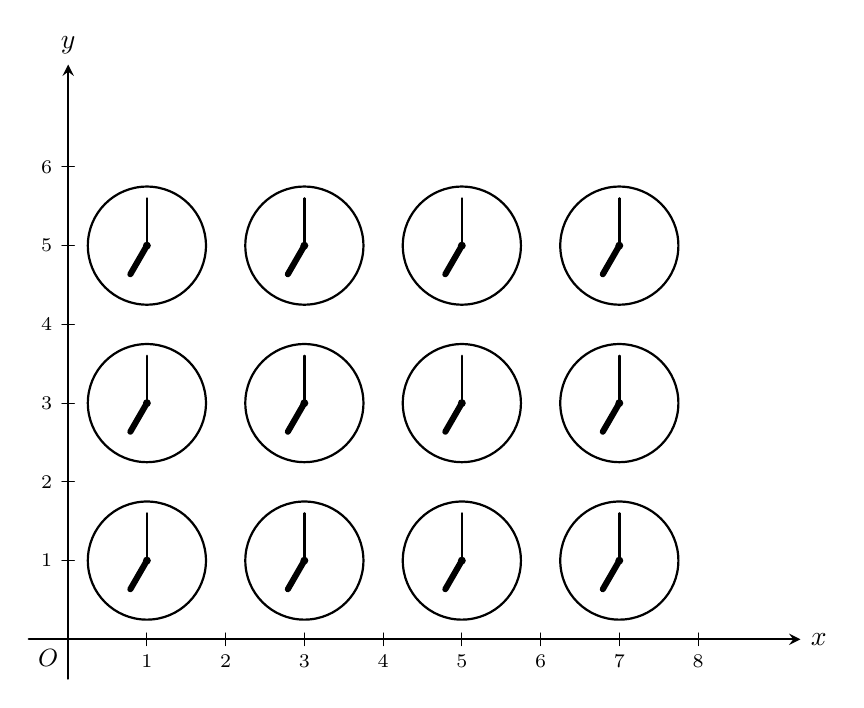
\begin{tikzpicture}[line cap=round, line join=round]

\def\R{0.75} % clock radius

%── Coordinate axes ───────────────────────────────────────────────────
\draw[-stealth, thick] (-0.5, 0) -- (9.3, 0) node[right] {$x$};
\draw[-stealth, thick] (0, -0.5) -- (0, 7.3) node[above] {$y$};
\node[below left, font=\small] at (0,0) {$O$};

\foreach \x in {1,...,8}
  \draw (\x, 0.08) -- (\x,-0.08) node[below, font=\scriptsize] {\x};
\foreach \y in {1,...,6}
  \draw (0.08,\y) -- (-0.08,\y) node[left, font=\scriptsize] {\y};

%── 12 clocks arranged in a 4 × 3 grid, all showing 19:00 ─────────────
%   At 19:00 (7 o'clock):
%     Minute hand → 0 min  →  12 o'clock  →  TikZ angle  90°
%     Hour   hand → 7 hrs  →  210° CW     →  TikZ angle 240°

\foreach \cx/\cy in {
    1/1, 3/1, 5/1, 7/1,
    1/3, 3/3, 5/3, 7/3,
    1/5, 3/5, 5/5, 7/5}
{
  % Clock face
  \fill[white]  (\cx,\cy) circle (\R);
  \draw[thick]  (\cx,\cy) circle (\R);

  % Minute hand — pointing to 12 (TikZ 90°), long and thin
  \draw[line width=0.9pt] (\cx,\cy) -- ++(90:0.60);

  % Hour hand — pointing to 7 (TikZ 240°), short and thick
  \draw[line width=2.2pt] (\cx,\cy) -- ++(240:0.42);

  % center pivot dot
  \fill (\cx,\cy) circle (0.05);
}

\end{tikzpicture}
\end{center}
Galilean transformation equations:
\[x'=x-vt;\ t'=t;\ u'=u-v\]
where $x$ and $x'$ denotes the position that the event occurred to two observers.
\begin{center}
  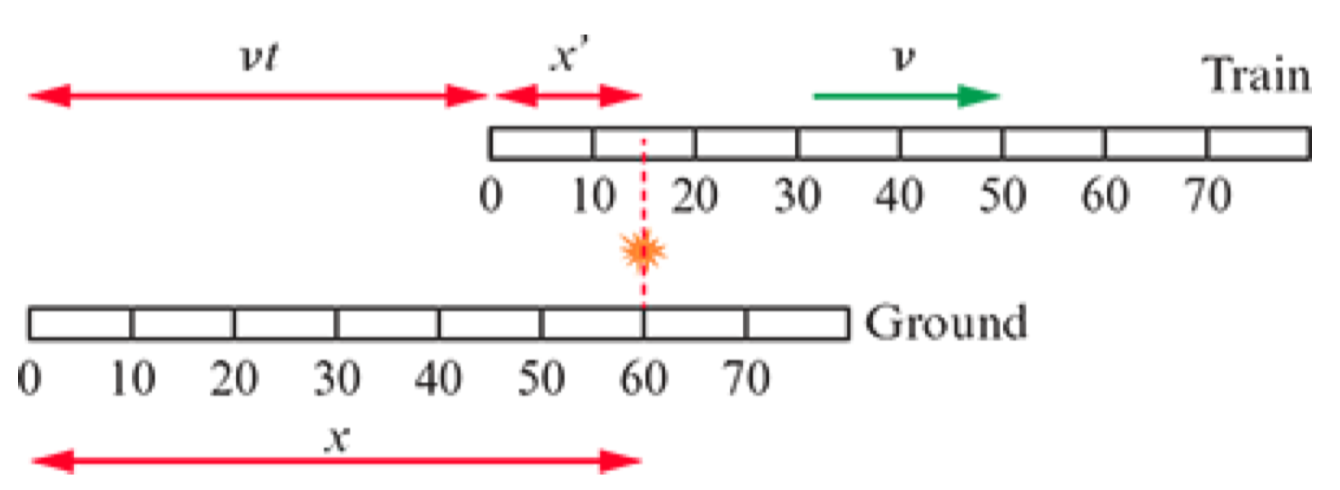
\includegraphics[width=0.6\linewidth]{截圖 2026-05-29 17.40.10.png}\\
  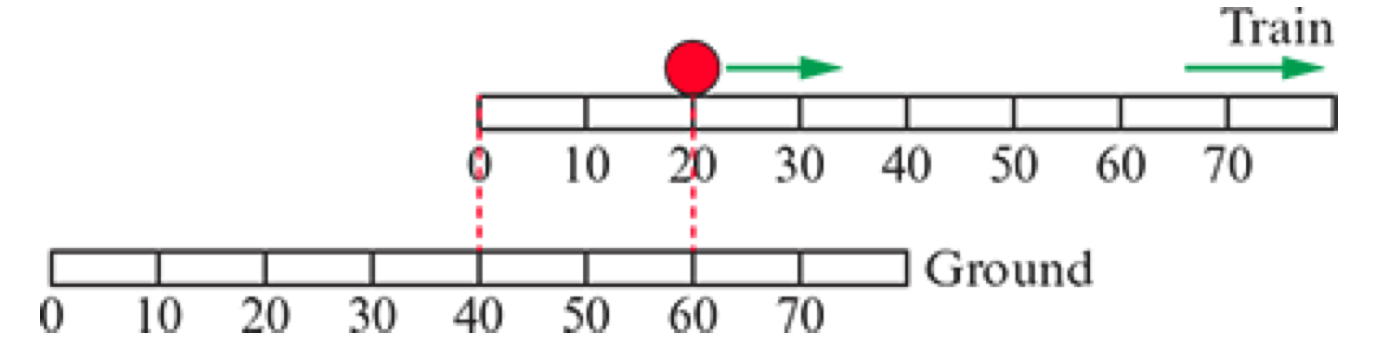
\includegraphics[width=0.6\linewidth]{截圖 2026-05-29 17.42.42.png}
\end{center}
Two observers always agree on what the time co-ordinates are; in other words, time is common to both observers.
\subsubsection*{The postulates of special relativity}
\begin{itemize}
  \item All the laws of physics are the same in all inertial frames.
  \item The speed of light in vacuum is the same for all inertial observers.
\end{itemize}
Lorentz transformations: (By Einstein, really)
\[x'=\gamma (x-vt);\ x=\gamma(x'+v't)\]
\[v'=\gamma\left(t-\dfrac{v}{c^2}x\right);\ v=\gamma\left(t'+\dfrac{v}{c^2}x'\right)\]
where $c$ is the speed of light and $\gamma$ is the gamma factor, $\displaystyle \gamma=\dfrac{1}{\sqrt{1-\dfrac{v^2}{c^2}}}$
\\If $v$ is very small
compared to the speed of light, then $\gamma\approx1$, the Lorentz equations reduce to
the Galilean equations. The effects of relativity become important only at speeds close to that of light.
\[\Delta x'=\gamma(\Delta x-v\Delta t);\ \Delta v'=\gamma(\Delta t-\dfrac{v}{c^2}\Delta x)\]
\[\Delta x=\gamma(\Delta x'+v\Delta t');\ \Delta v=\gamma(\Delta t'+\dfrac{v}{c^2}\Delta x')\]
\subsubsection*{Spacetime interval}
A quantity that both observers will agree on. Mathematically speaking,
\[(\Delta s)^2=(\Delta s')^2 \Rightarrow (c\Delta t)^2-(\Delta x)^2=(c\Delta t')^2-(\Delta x')^2\]
\subsection{Effects of relativity}
\subsubsection*{Time dilation} the interval between the ticks of a clock that moves relative to the observer in $S$ is greater than the interval measured in $S'$ where the clock is at rest.\\
When $\Delta x'=0$, $\Delta t=\gamma \Delta t'$. In a straightforward way,
\[\text{time interval}=\gamma\times \text{proper time interval}\]
where proper time interval is the time between two events that take place at the same point in space.
\subsubsection*{Length contraction}
\[L=\dfrac{L_0}{\gamma}\]
Note that it is only lengths in the direction of motion that are contracted.\\
$L_0$ is the proper length, the length of the rod at rest in the rest frame, frame $S'$, $\Delta x'$.\\
$L$ is the length of the rod in frame $S$, $\Delta x$.
\subsubsection*{Addition of velocities}
Consider a frame $S'$ that moves at constant speed $v$ in a straight line relative to another frame $S$. Observers in both frames measure the velocity of an object. Observers in $S'$ measure the velocity to be $u'$. Observers in $S$ measure the velocity of the same object to be $u$. How are $u$ and $u'$ related?
\[u=\dfrac{u'+v}{1+\dfrac{u'v}{c^2}};\ u'=\dfrac{u-v}{1-\dfrac{uv}{c^2}}\]
\subsubsection*{Simultaneity}
Suppose that as usual we have frames S and $S'$ with frame $S'$ moving to the right with speed $v$ relative to $S$. Suppose that two events take place at the same time in frame $S'$, $\Delta t' = 0$. The time interval between the same two events when measured in S is:
\[\Delta t=\gamma\dfrac{v}{c^2}\Delta x'\]
\begin{itemize}
  \item Events that are simultaneous for one observer and which take place at different points in space, are not simultaneous for another observer in motion relative to the first. $\Delta x'\neq 0$
  \item If two events are simultaneous for one observer and take place at the same point in space, they are simultaneous for all other observers as well. $\Delta x'=0$
\end{itemize}
\subsubsection*{Muon decays}
Muons are particles with properties similar to those of the electron except that they are more massive, are unstable and decay into electrons.
They have an average lifetime of $2.2\times 10^{-6}\ \text{s}$, and is the proper time interval between its creation and its decay.\\
From the point of view of an observer in the laboratory, however, the muons are moving at high speed; the lifetime is longer because of time dilation.\\
想象这个$\mu$子从一个（3公里高的）山上发射下来（比如说他有$0.99c$的速度），地上有一个接收器。在相对论的影响下，对于观测者而言时间被减慢了（$\Delta t=\gamma \times 2.2\times 10^{-6}\ \text{s}=1.56\times10^{-5}\ \text{s}$），对于观测者而言穿越的路程增加了（4.63 km），因此$\mu$子可以在被接收器接收之后再衰变。没有相对论的影响$\mu$子就只能走0.653公里，显然不足以支撑它坚持到检测器的检测。\\
对于一个在$\mu$子上的观测者（我们就假设真的有这样一个观测者），是地球在向上移动，因此这个山的距离对于他只有0.42公里，需要$1.4\times10^{-6}$秒的时间遇上检测器。所以说，In this sense, muon decay experiments are direct confirmations of time dilation and indirect confirmations of length contraction.
\begin{center}
  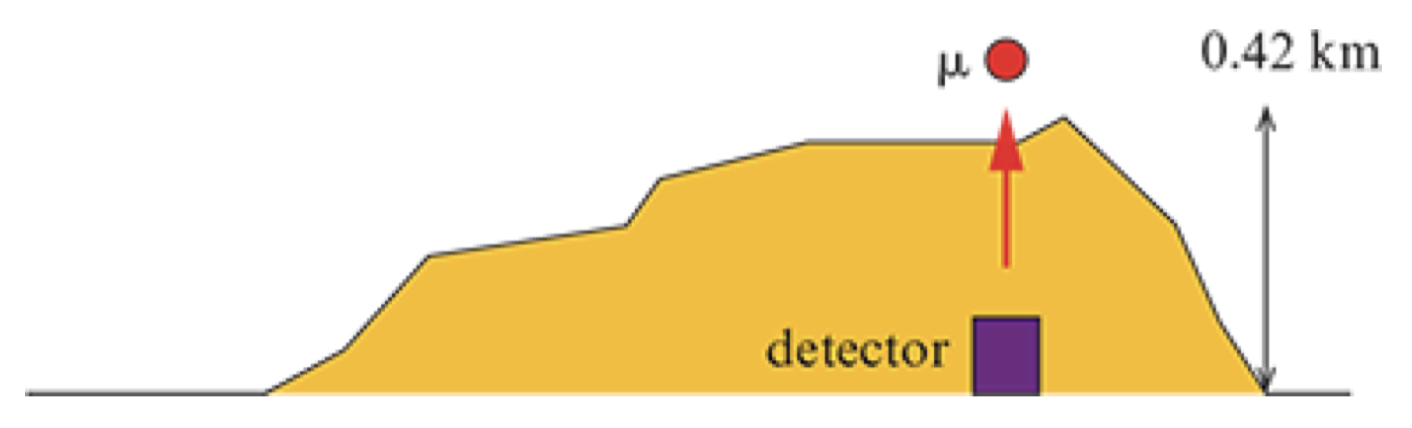
\includegraphics[width=0.7\linewidth]{Screenshot 2026-07-11 at 10.10.53.png}
\end{center}
\subsection{Spacetime / Minkowski diagrams}
Do not be led astray by your knowledge of Euclidean geometry! \\
Time is the y-axis (plotted as $ct$ though, in meters), distance (1D) is the x-axis.
\begin{center}
\begin{tikzpicture}[
    scale=1.2,
    >=Stealth,
    font=\small,
    axis/.style={thick,->},
    worldline/.style={thick,blue},
    lightcone/.style={dashed,thick,red}
]

% Draw axes
\draw[axis] (-0.5,0) -- (5,0) node[below right] {Space \(x\)};
\draw[axis] (0,-0.5) -- (0,5) node[above left] {Time \(ct\)};
% Add a few grid lines (optional, helps see coordinates)
\draw[help lines, gray!30] (-0.5,-0.5) grid (5,5);

% Label the axes with arrows
\draw[->] (0,0) -- (5,0) node[below] {\(x\)};
\draw[->] (0,0) -- (0,5) node[left] {\(t\)};
\draw[color=red] (0,0) -- (2,4) node[right] {worldline of a moving particle};
\draw[color=blue] (4,0) -- (4,3) node[right] {worldline of a particle at rest};
\fill (0,0) circle (2pt) node[below left] {Event \(O\)};
\node[label, above, color=red] at (0.25,0.8) {$\theta$};
\end{tikzpicture}
\end{center}
The tangent of the angle between the worldline and the ct axis gives the speed divided by the speed of light. Since nothing can exceed c, the worldline of any particle will always make
an angle less than $45^\circ$ with the ct axis.\\
\begin{center}
  \resizebox{0.5\textwidth}{!}{%
  \begin{tikzpicture}[
    scale=1.2,
    >=Stealth,
    font=\small
]

% Axes
\draw[thick,->] (-4.5,0) -- (4.5,0) node[below] {Space \(x\)};
\draw[thick,->] (0,-4.7) -- (0,4.7) node[left] {Time \(ct\)};

% Past light cone (blue) - goes backward in time (downward), but we draw from apex at origin upward? 
% Actually past light cone is the set of events that can send light to the origin. 
% So from origin, draw lines downward (negative time) with slopes ±1. 
% But to show both cones clearly, we draw the past cone extending downward from origin.
% For aesthetic, draw both cones symmetric about the horizontal axis? Usually time is vertical upward, so past is below origin.
% I'll draw: future cone (yellow) from origin going upward at ±45°, past cone (blue) from origin going downward at ±45°.

% Future light cone (yellow) - upper half
\draw[thick, yellow!80!orange] (0,0) -- (4,4.5);
\draw[thick, yellow!80!orange] (0,0) -- (-4,4.5);

% Past light cone (blue) - lower half
\draw[thick, blue] (0,0) -- (4,-4.5);
\draw[thick, blue] (0,0) -- (-4,-4.5);

% Optional: fill the cones with translucent color to emphasize "cone"
% This makes it look nicer but might be too much. I'll add light fill with opacity.
\fill[yellow!20, opacity=0.5] (0,0) -- (4,4.5) -- (-4,4.5) -- cycle;
\fill[blue!20, opacity=0.5] (0,0) -- (4,-4.5) -- (-4,-4.5) -- cycle;

% Label the origin event
\fill (0,0) circle (2pt);
\node [below, right] at (0.4, -0.25) {Present event};

% Add small labels for the cones
\node[yellow!80!orange, above right] at (2.5,2.5) {Future light cone};
\node[blue, below right] at (2.5,-2.5) {Past light cone};

% Light rays (45° lines) are already drawn; add a note about slope = c
\node[black, below] at (3.5,0.5) {\(45^\circ\) (speed of light)};

\end{tikzpicture}
  }%
\end{center}
The region coloured yellow consists of all events that can be influenced by event E. Similarly, events that could have influenced E are within the region coloured blue.\\\\
重要概念：其实坐标轴可以是斜的。想象有一个$S'$以$v$的速度向右移动，且$S$和$S'$的原点重合。$ct'$的坐标轴会和$ct$坐标轴形成$\theta=\tan^{-1}\left(\dfrac{v}{c}\right)$的夹角。同样地，$x'$的坐标轴会和$x$坐标轴形成$\theta$的夹角。所有坐标轴均对称于光子的世界线（因为光速在所有的Frames里的速度都是一致的）。\\\\
Use the gamma factor and Lorentz transformation to find $x$ and $ct$ from $x'$ and $ct'$ values. ($x=\gamma(x'+vt')$, $ct=\gamma(ct'+vcx')$) 当$x$和$ct$等于伽马系数的时候，向右/向上延伸与$ct'$和$x'$相交的点就是$S'$下的1m。
\subsubsection*{Length contraction}
\begin{center}
  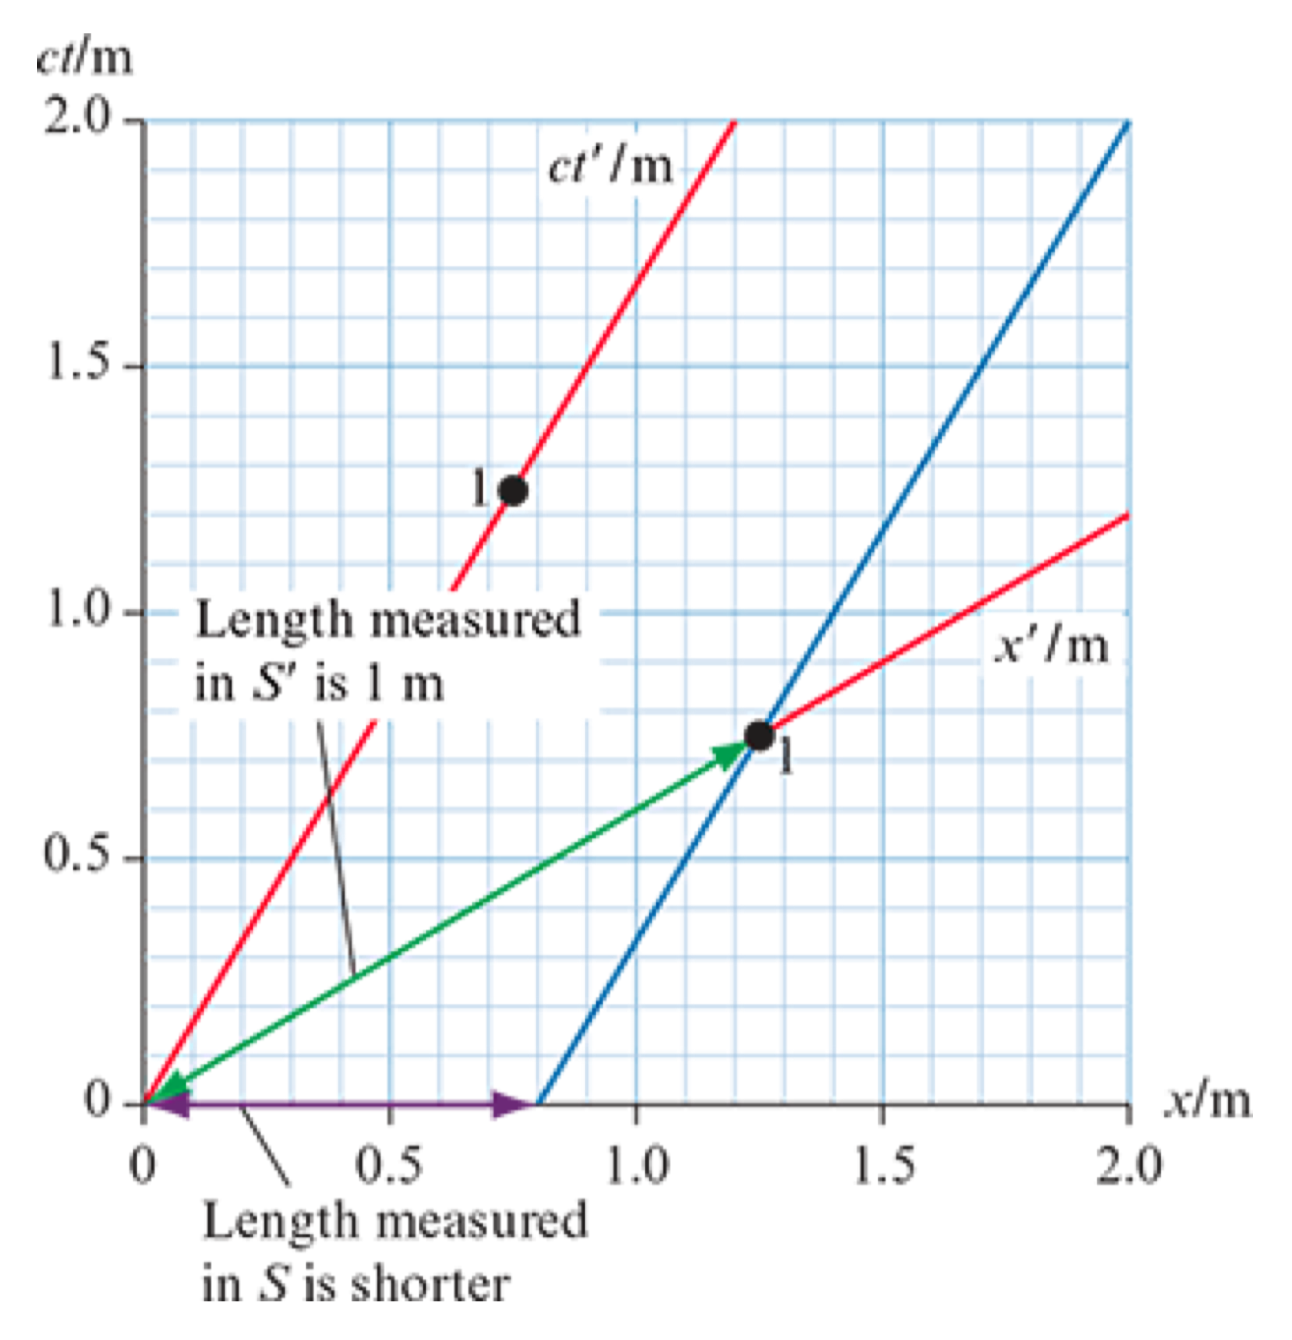
\includegraphics[width=0.45\linewidth]{截圖 2026-05-30 13.58.36.png}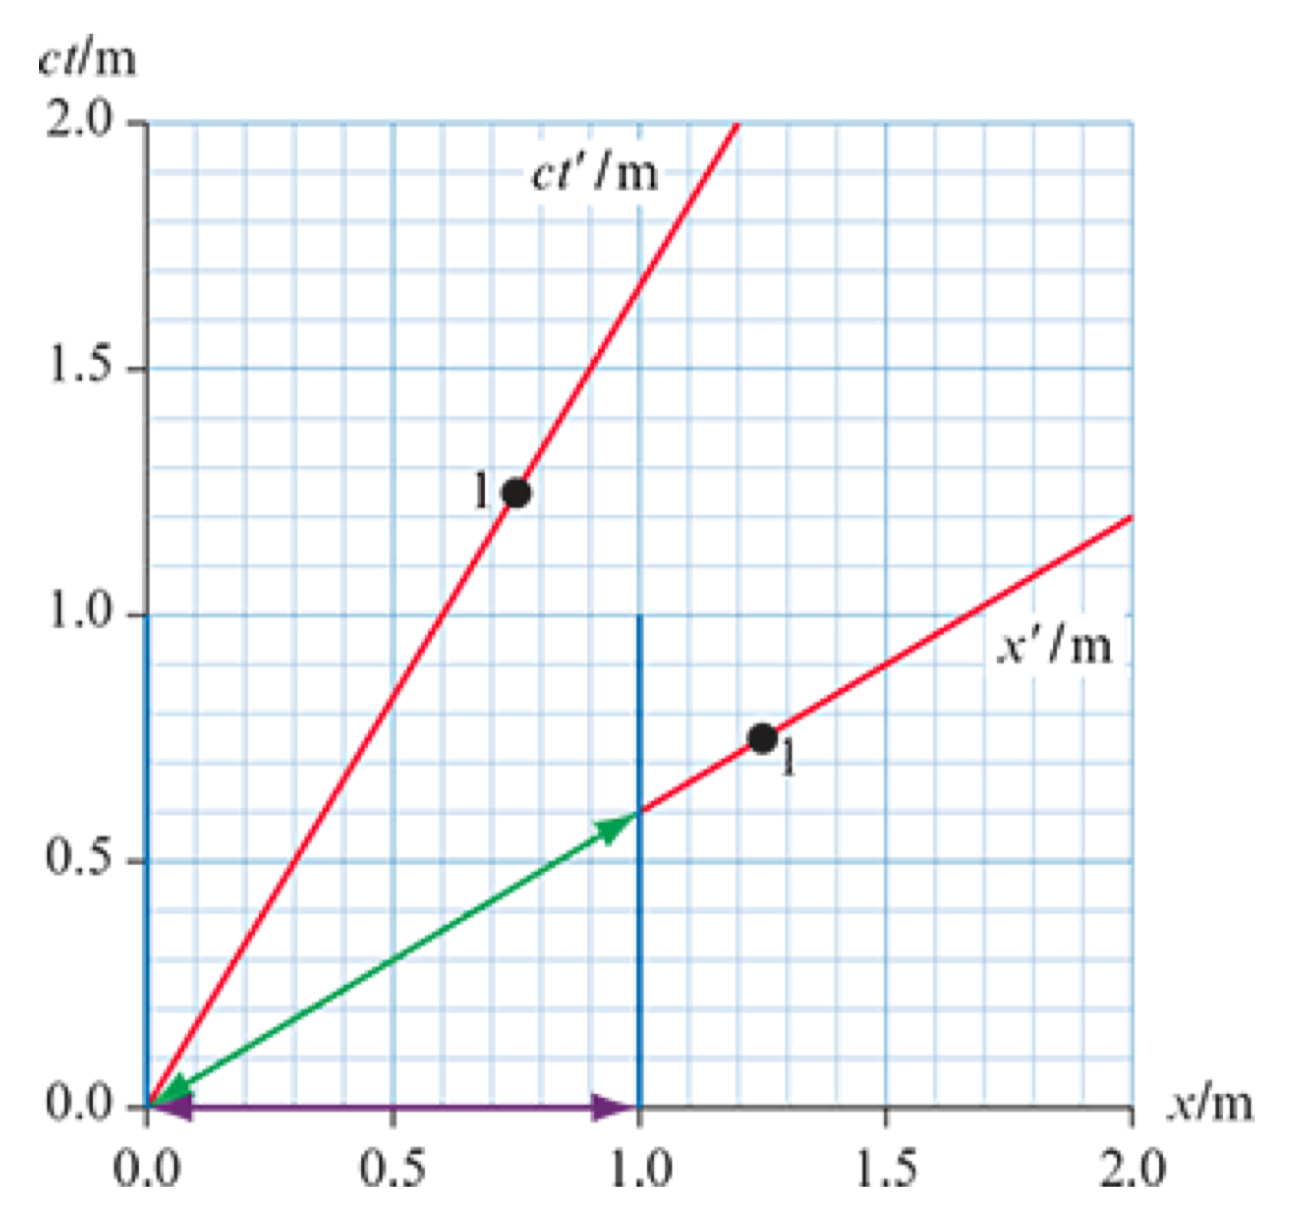
\includegraphics[width=0.5\linewidth]{截圖 2026-05-30 14.00.22.png}
\end{center}
If the rod is moving its length must be measured when the position of its ends are recorded at the same time.
It is only lengths in the direction of the velocity that are contracted.
\subsubsection*{Time dilation}
\begin{center}
  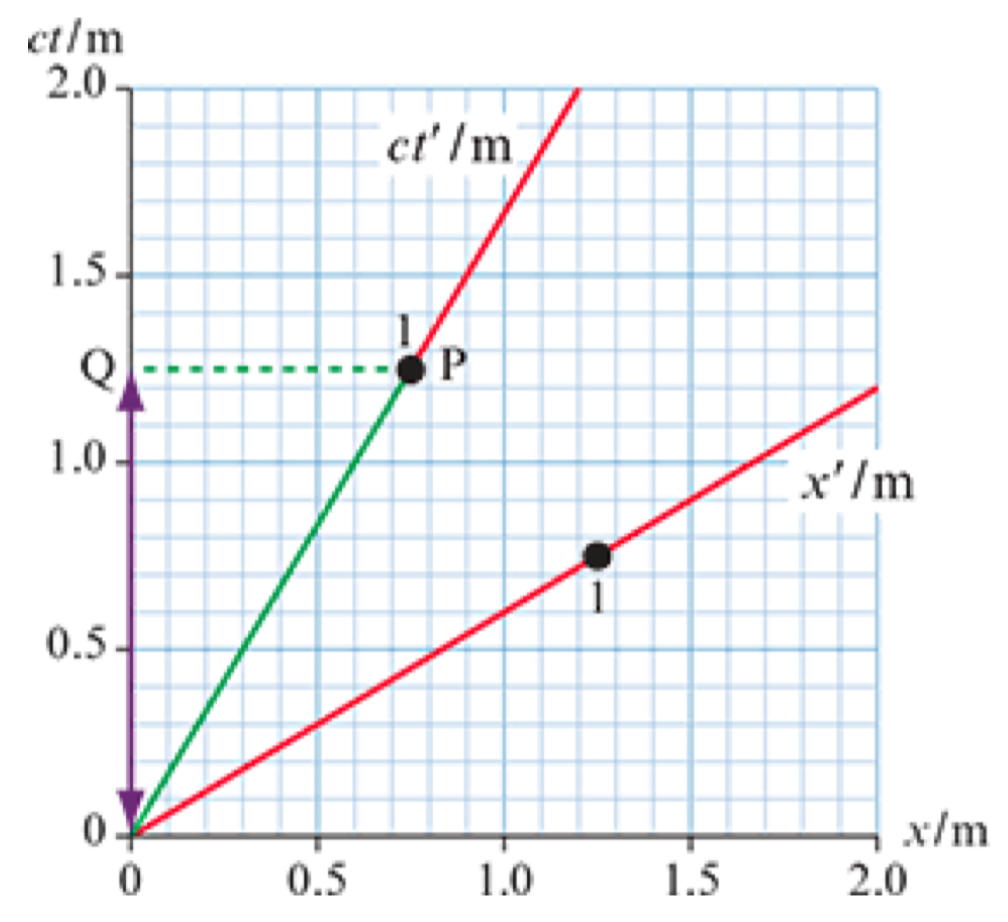
\includegraphics[width=0.45\linewidth]{截圖 2026-05-30 14.04.03.png}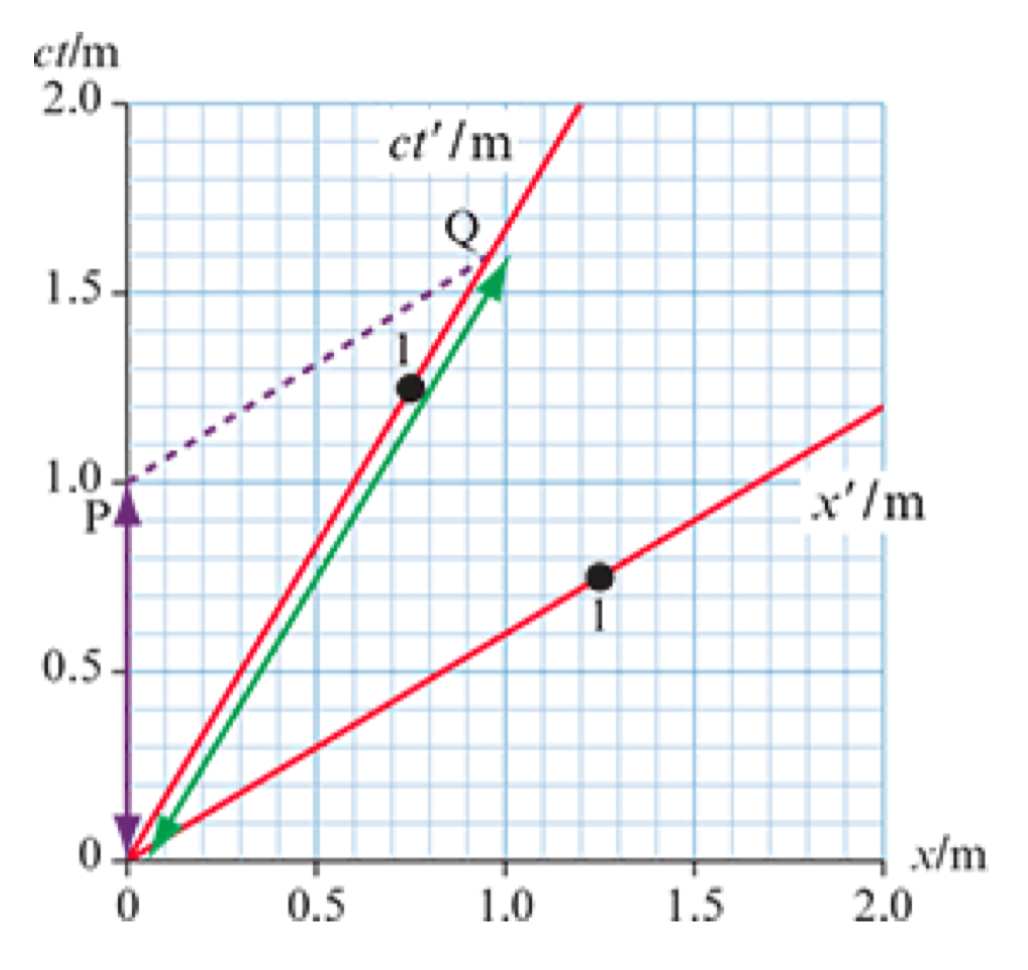
\includegraphics[width=0.45\linewidth]{截圖 2026-05-30 14.04.25.png}
\end{center}
$^*:$ PQ in the second diagram is parallel to the $x'$ axis.
\subsubsection*{Simultaneity}
Events happen simultaneously in an arbitrary frame $S$ if the $ct$ value are the same for both events (lines on the same line parallel to the $x$ axis).
\begin{center}
  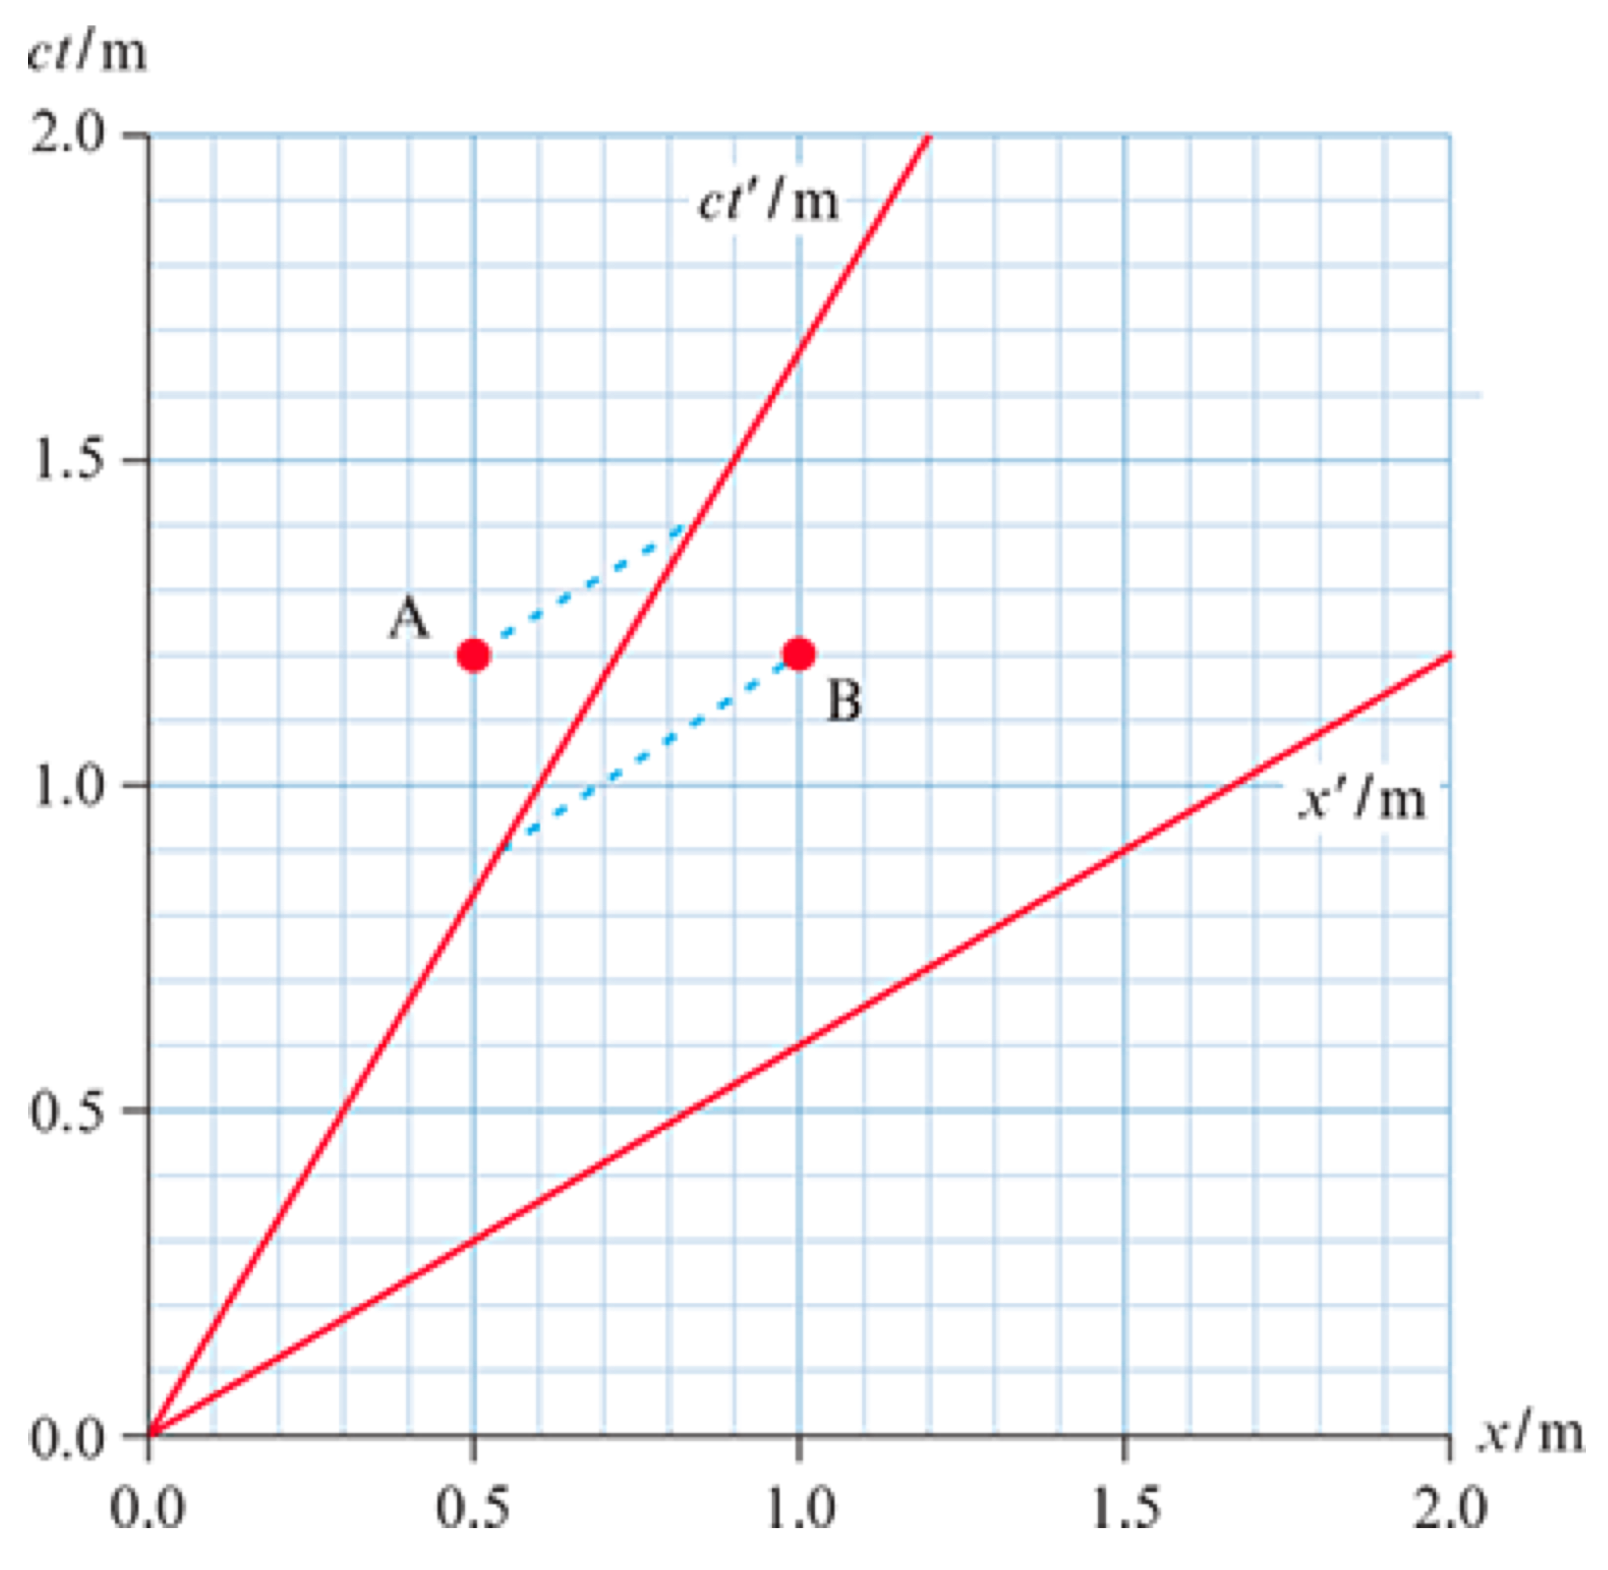
\includegraphics[width=0.45\linewidth]{截圖 2026-05-30 14.15.16.png}
\end{center}
To find out how much earlier an event (B for example) occurs use a Lorentz transformation:
\[c\Delta t'=\gamma(c\Delta t-\dfrac{v}{c}\Delta x)\]
This is really just a transformed form of this equation:
\[\Delta t=\gamma\dfrac{v}{c^2}\Delta x'\]
\newpage
% ===================== Unit B =====================
\unnumberedsection{Unit B The particulate nature of matter}
\section{Thermal energy transfers}
\subsection{Particles, temperature and energy}
States of matter: solid, liquid, gas.
\begin{center}
\begin{tabularx}{\textwidth}{@{}|Y |Y |Y| Y|@{}}
\toprule
\textbf{Property} & \textbf{Solid} & \textbf{Liquid} & \textbf{Gas} \\
\midrule
Forces between particles & Strong & Weaker than solids, but still significant & Very weak (negligible except during collisions) \\\hline
Particle motion & Fixed; Very difficult to break apart & Move around each other; flows, takes container shape & Free motion; forces only during collisions \\\hline
Compressibility & Very nearly incompressible & Very nearly incompressible & Highly compressible \\\hline
Interparticle distance & Small (reference) & Similar to solids & About 10× larger than in solids/liquids \\\hline
Typical density (kg\,m$^{-3}$) & $7.8\times10^3$ (iron) & $6.9\times10^3$ (liquid iron) & $1.2$ (air, depends on $T$ and $P$) \\\hline
Density comparison & Comparable to liquids & Comparable to solids & $\sim$1000× smaller \\\hline
Intermolecular potential energy & Large negative (deep potential well); & Negative but shallower than solids; & Approximately zero (negligible interactions) \\
\bottomrule
\end{tabularx}
\end{center}
Formula for calculating density: $\rho=\dfrac{m}{V}$. \\
Temperature (in kelvin) is proportional to the average random kinetic energy of the molecules.
\[\overline{E}_K=\dfrac{3}{2}k_BT\]
where $k_B=1.38\times 10^{-23}\ \text{J\,K}^{-1}$, the Boltzmann constant. This direct proportionality between temperature and the average random kinetic energy is only true for the absolute or kelvin temperature scale.\\
\[T\text{ (in K) }=T\text{ (in $^\circ C$) }+273\]
Thermal energy is the energy that gets transferred from one body to another as a result of a temperature difference.
When two bodies are in contact and have different temperatures, there will be a transfer of thermal energy from the hotter to the colder body.
\\\\
Internal energy of a substance is defined as the total random kinetic energy of the particles of a substance, plus the total intermolecular potential energy of the particles. The internal energy of a system can change as a result of thermal energy added or taken out but also as a result of work performed. 
\\\\
We need to do work to increase the separation of the particles in a solid. This work goes into intermolecular potential energy, $E_p$. The average separation of the molecules corresponds to the minimum of the curve, about 1.2 nm for this graph. For separations larger than 1.2 nm the forces between molecules are attractive. For smaller separations, the forces are repulsive, indicating that the molecules cannot get that close to each other. For gas, the potential energy is 0.
\begin{center}
  \begin{tikzpicture}
\begin{axis}[
    xlabel = Distance $r$ (nm),
    ylabel = $E_p$,
    xlabel style = {anchor=west},
    ylabel style = {anchor=south},
    axis lines = middle,
    xtick = {1.2},
    xticklabels = {$r_0$},
    ytick = {-1},
    yticklabels = {$-\varepsilon$},
    ymin = -1.2,
    ymax = 1.5,
    xmin = 0.0,
    xmax = 3.2,
    width = 15cm,
    height = 8cm,
    samples = 200,
    domain = 1.03:3.2,
    restrict y to domain = -1.5:3,
    clip = false,
]
% Lennard-Jones type: scaled so min = -1 at r=1.2
\addplot [thick, smooth] { (1.2/x)^12 - 2*(1.2/x)^6 };

% Optional curve label
\node [anchor=south west, font=\small] at (axis cs:2.2,0.3) 
    {$E_p(r) = 4\varepsilon\left[\left(\frac{\sigma}{r}\right)^{12}-\left(\frac{\sigma}{r}\right)^6\right]$};
\end{axis}
\end{tikzpicture}
\end{center}
\subsection{Specific heat capacity and change of phase}
Specific heat capacity: the energy required to increase the temperature of a unit mass of the body by one kelvin.
\[Q=mc\Delta t\]
where $Q$ is the amount of heat needed, $m$ is the mass, $\Delta t$ is the change in temperature.\\\\
Changes of phases:
\begin{itemize}
  \item melting: when a solid changes to a liquid (thermal energy is transferred to the solid)
  \item freezing: when a liquid changes into a solid (thermal energy is transferred away from the liquid)
  \item vaporisation (or boiling): when a liquid changes into vapour (thermal energy is transferred to the liquid)
  \item condensation: when a vapour changes into a liquid (thermal energy is transferred away from the vapour).
  \item evaporation: vaporisation taking place at the surface of a liquid at any temperature (rate increases with higher surface area and higher temperature)
\end{itemize}
Latent heat: The energy supplied or removed during a phase change (does not increase / decrease the temperature of the substance)\\
Specific latent heat: the energy required to change the phase of 1 kg of a substance at constant temperature and pressure.
\[Q=mL\]
where $m$ is the mass, $Q$ is the energy applied, $L_F$ is the \textbf{specific latent heat of fusion} (for melting / freezing), $L_V$ is the \textbf{specific latent heat of vaporization} (for vaporization / condensation)\\
Generally speaking, $L_V>L_F$.\\\\
What happens during change in phase:
\begin{itemize}
  \item The thermal energy supplied increases the intermolecular potential energy, internal energy increases
  \item This work increases the separation of the molecules
  \item The average distance between the molecules increases
  \item Change in phase occurred
\end{itemize}
The transfer of thermal energy between (melted) water and ice ensures that the overall equilibrium temp-\\erature stays at 0$^\circ$C.\\\\
Two methods for measuring specific heat capacity:
\begin{itemize}
  \item Electrical method
  \begin{enumerate}
    \item Record initial temperature of the substance
    \item Apply heat from electrical heater (with known power / voltage + current) for a certain amount of time
    \item Measure the final temperature, calculate specific heat capacity
  \end{enumerate}
  \item Method of mixtures
  \begin{enumerate}
    \item A solid is put in a container of hot water and allowed time to reach a constant temperature
    \item The temperature of the solid is recorded (equal to temperature of water)
    \item The solid is then transferred into an insulated calorimeter 热量计 of known specific heat capacity and initial temperature which contains a liquid
    \item Final temperature of water is then recorded (when thermal equilibrium reached)
    \item \[\underbrace{Q}_\text{substance with unknown $c_{sp}$}=\underbrace{Q}_\text{calorimeter}+\underbrace{Q}_\text{liquid (water)}\]
    $L_F / L_V$ could also be calculated this way:
    \[\underbrace{Q}_\text{latent heat} + \underbrace{Q}_\text{heat for change in temperature}=\underbrace{Q}_\text{calorimeter}+\underbrace{Q}_\text{liquid (water)}\]
    \item (It is likely that some thermal energy (heat) was dissipated to the surrounding air, therefore the real $c_{sp}$ might be larger than the calculated value)
  \end{enumerate}
\end{itemize}
The rate of cooling is proportional to the difference in temperature between the liquid and the surroundings:
\[\dfrac{\Delta T}{\Delta t}=k(T-T_s)\]
where the constant $k$ is proportional to the area of the surface of the liquid.\\
(This implies an exponential decrease of temperature)
\subsection{Thermal energy transfer}
\begin{itemize}
  \item Conduction
  \begin{itemize}
    \item The moving electrons collide with neighbouring molecules, transferring energy to them and so increasing their average kinetic energy.
\begin{center}

\begin{tikzpicture}[
    scale=0.6,
    transform shape,
    >=Latex,
    line join=round,
    line cap=round
]

%--------------------------------------------------
% Parameters
%--------------------------------------------------

\def\H{4}
\def\W{2}
\def\D{2}

\def\Gap{2.2}

%--------------------------------------------------
% HOT BLOCK
%--------------------------------------------------

\fill[red!15]
(0,0) -- (\W,0) -- (\W,\H) -- (0,\H) -- cycle;

\fill[red!20]
(\W,0) -- (\W+1,\D) -- (\W+1,\H+\D) -- (\W,\H) -- cycle;

\fill[red!10]
(0,\H) -- (\W,\H) -- (\W+1,\H+\D) -- (1,\H+\D) -- cycle;

\draw[black,thick]
(0,0) -- (\W,0) -- (\W,\H) -- (0,\H) -- cycle;

\draw[black,thick]
(\W,0) -- (\W+1,\D);
\draw[black,thick]
(\W,\H) -- (\W+1,\H+\D);
\draw[black,thick]
(\W+1,\D) -- (\W+1,\H+\D);
% Hot block: back-left vertical edge
\draw[black,thick] (0,2+\D) -- (1,\H+2);
\draw[black,thick]
(1,\H+\D) -- (\W+1,\H+\D);

\node[align=center] at (1,1.6)
{$T_H$\\hot};

%--------------------------------------------------
% CONDUCTION SLAB
%--------------------------------------------------

\fill[red!8]
(\W,0.8)
--
(\W+\Gap,0.8)
--
(\W+\Gap+1,\D+0.8)
--
(\W+1,\D+0.8)
-- cycle;

\fill[red!8]
(\W,2.6)
--
(\W+\Gap,2.6)
--
(\W+\Gap+1,\D+2.6)
--
(\W+1,\D+2.6)
-- cycle;

\draw[black]
(\W,0.8) -- (\W+\Gap,0.8);

\draw[black]
(\W,2.6) -- (\W+\Gap,2.6);

%--------------------------------------------------
% COLD BLOCK
%--------------------------------------------------

\begin{scope}[shift={(\W+\Gap,0)}]

\fill[cyan!25]
(0,0) -- (\W,0) -- (\W,\H) -- (0,\H) -- cycle;

\fill[cyan!50]
(\W,0) -- (\W+1,\D) -- (\W+1,\H+\D) -- (\W,\H) -- cycle;

\fill[cyan!15]
(0,\H) -- (\W,\H) -- (\W+1,\H+\D) -- (1,\H+\D) -- cycle;

% Draw ALL edges

\draw[black,thick]
(0,0) -- (\W,0) -- (\W,\H) -- (0,\H) -- cycle;

\draw[black,thick]
(\W,0) -- (\W+1,\D);

\draw[black,thick]
(\W,\H) -- (\W+1,\H+\D);

\draw[black,thick]
(\W+1,\D) -- (\W+1,\H+\D);

\draw[black,thick]
(1,\H+\D) -- (\W+1,\H+\D);


% Cold block: back-left vertical edge
\draw[black,thick] (0,\D+2) -- (1,\H+2);
\node[align=center] at (1,2)
{$T_C$\\cold};

\end{scope}

%--------------------------------------------------
% Q arrows
%--------------------------------------------------

\foreach \y in {1.0,1.8,2.6}
{
    \draw[red,ultra thick,-Latex]
    (\W+0.35,\y)
    --
    (\W+\Gap-0.35,\y);
}

\node at (\W+0.9,3.15) {$Q$};

%--------------------------------------------------
% Delta x
%--------------------------------------------------

\draw[thick,<->]
(\W,-0.6)
--
(\W+\Gap,-0.6);

\node at (\W+\Gap/2,-1.05)
{$\Delta x$};
\end{tikzpicture}
\end{center}
    \item Molecules on the hot side of the solid vibrate about their equilibrium positions, stretching the bonds with neighbouring molecules. This stretching forces the neighbours to also begin to vibrate, and so the average kinetic energy of the neighbours increases. Energy is again transferred.
    \item \[\dfrac{\Delta Q}{\Delta t}=kA\dfrac{\Delta T}{\Delta x}\] where $k$ is the conductivity, $A$ is the cross-sectional area, $\Delta x$ is the width, $\Delta T$ is the temperature difference, $\Delta T=T_H-T_C$.
  \end{itemize}
  \item Convection
  \begin{itemize}
    \item Applies to fluids (liquids and gases)
    \item Hotter liquids are less dense / hotter gases would expand and rise, colder fluids are more dense and sink
    \item This process preforms continuously to form the convection currents
    \begin{center}
      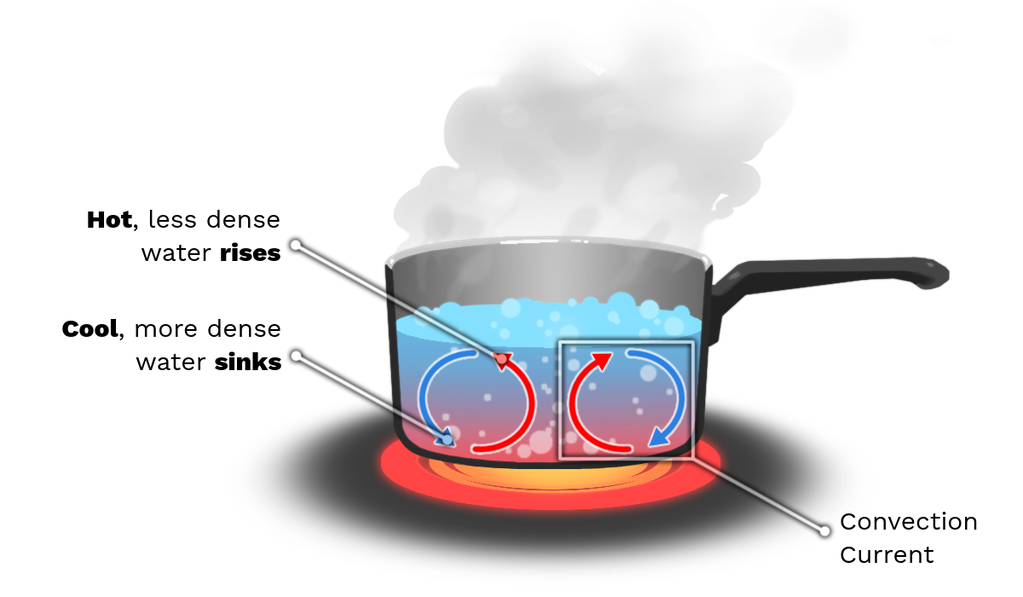
\includegraphics[width=0.5\linewidth]{DOT_Convection.en.x1024.png}
    \end{center}
  \end{itemize}
  \item Radiation
  \begin{itemize}
    \item Does not require a medium for the transfer of thermal energy -- can occur in vacuum
    \item Radiate energy in forms of EM waves, radiation created by oscillating electric charges in the atoms of the body.
    \item Stefan-Boltzmann Law: The power radiated by a black body is given by \[P=\sigma AT^4\] where $A$ is the surface area, $T$ is the absolute temperature of the surface, $\sigma$ is the Stefan-Boltzmann constant, $\sigma=5.67\times10^{-8}\ \text{W\,m}^{-2}\,\text{K}^{-4}$
    \item The radiated intensity (power radiated per unit area of the body) is thus $\dfrac{P}{A}=\sigma T^4$
    \item Strictly, this applies to a theoretical body called a black body. This is a perfect radiator as well as a perfect absorber. A black body at low temperature radiates very little, and since it absorbs all the radiation falling on it, it looks black. At high temperature it radiates a lot and looks very bright.
  \end{itemize}
\end{itemize}
\begin{center}
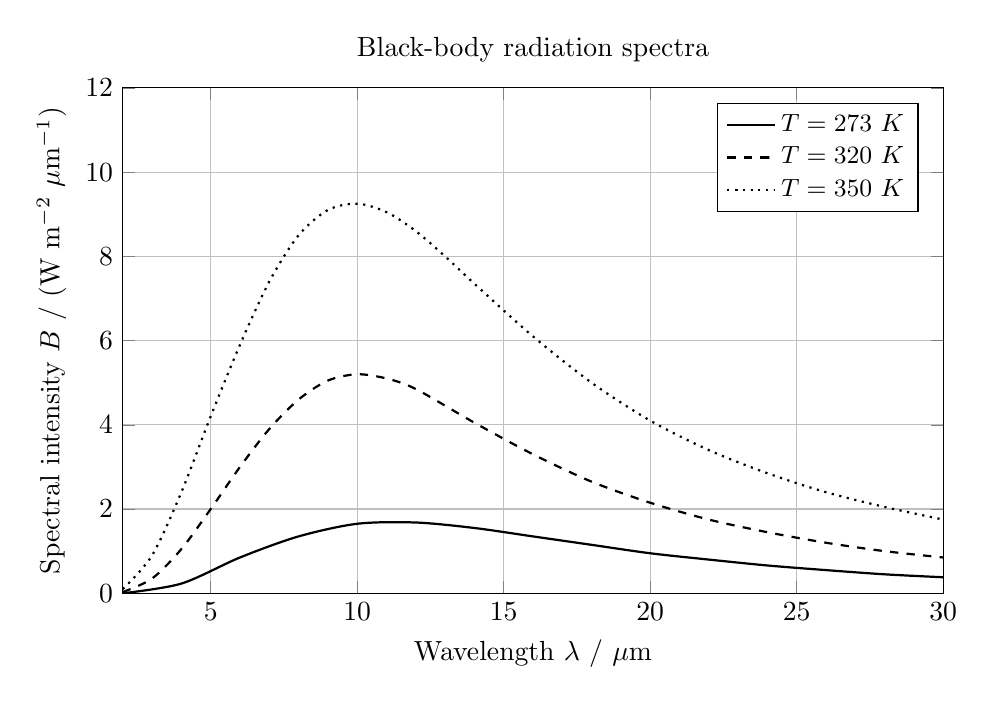
\begin{tikzpicture}
\begin{axis}[
    xlabel = Wavelength \(\lambda\) / \(\mu\)m,
    ylabel = Spectral intensity \(B\) / (W m\(^{-2}\) \(\mu\)m\(^{-1}\)),
    domain = 2:30,
    grid = both,
    minor grid style = {draw=gray!25},
    width = 12cm,
    height = 8cm,
    legend pos = north east,
    legend style = {font=\small, cells={anchor=west}},
    xmin = 2, xmax = 30,
    ymin = 0,
    ymax = 12,    % adjust if needed
    title = Black-body radiation spectra,
]

% 273 K (scaled for visualisation; actual values are much smaller)
\addplot[thick, smooth] coordinates {
    (2, 0.0001) (4, 0.23)   (6, 0.85)   (8, 1.35)
    (10, 1.65)  (12, 1.68)  (14, 1.55)  (16, 1.35)
    (18, 1.15)  (20, 0.95)  (22, 0.80)  (24, 0.66)
    (26, 0.55)  (28, 0.45)  (30, 0.38)
};

% 320 K (peak ~9.0 µm, higher intensity)
\addplot[thick, smooth, dashed] coordinates {
    (2, 0.03)   (3, 0.35)   (4, 1.05)   (5, 2.00)
    (6, 3.00)   (7, 3.90)   (8, 4.60)   (9, 5.05)
    (10, 5.20)  (11, 5.10)  (12, 4.85)  (14, 4.05)
    (16, 3.30)  (18, 2.65)  (20, 2.15)  (22, 1.75)
    (24, 1.45)  (26, 1.20)  (28, 1.00)  (30, 0.85)
};

% 350 K (peak ~8.2 µm, highest intensity)
\addplot[thick, smooth, dotted] coordinates {
    (2, 0.10)   (3, 0.90)   (4, 2.40)   (5, 4.20)
    (6, 5.90)   (7, 7.40)   (8, 8.50)   (9, 9.10)
    (10, 9.25)  (11, 9.05)  (12, 8.60)  (13, 8.00)
    (14, 7.35)  (16, 6.10)  (18, 5.00)  (20, 4.10)
    (22, 3.40)  (24, 2.85)  (26, 2.40)  (28, 2.05)
    (30, 1.75)
};

\legend{\(T = 273\ \text{K}\), \(T = 320\ \text{K}\), \(T = 350\ \text{K}\)}

\end{axis}
\end{tikzpicture}\\
\(^*:\) Spectral intensity: power emitted per unit area per unit wavelength
\end{center}
The area under the graph is the radiated intensity. With increasing temperature, the peak of the curve occurs at lower wavelengths and the height of the peak increases. The energy radiated is electromagnetic radiation and is distributed over an infinite range of wavelengths. The peak of the spectrum corresponds to a specific wavelength $\lambda_\text{max}$, called the peak wavelength.
\\\\Wien's Law: \[\lambda_\text{max}T=2.90\times 10^{-3}\ \text{K\,m}\] This shows that the peak wavelength $\lambda_0$ depends on temperature.\\\\
Apparent brightness (the power received per unit area of the detector):
\[B=\dfrac{L}{4\pi d^2}=\dfrac{\sigma AT^4}{4\pi d^2}\] where $L$ is the luminosity of the star, $d$ is the distance from the star to the observer.\\
Luminosity of a star is given by 
\[L=\sigma AT^4\]
where $A$ is the surface area of the star, $T$ is the temperature of the star.
\section{The greenhouse effect}
\subsection{Radiation from real bodies}
Real bodies radiate according to the modified Stefan-Boltzmann law:
\[P=e\sigma AT^4\]
where $e$ is the emissivity of the body, a number between 0 and 1, the ratio of the power per unit area radiated by a body to the power per unit area radiated by a black body of the same temperature. A perfect black body has an emissivity of 1, while a perfect reflector has an emissivity of 0.\\
The power radiated per unit area is called (radiated) intensity, and is equal to $I=e\sigma T^4$.\\
Albedo of the body is the ratio of the reflected intensity (or power) to the incident intensity (or power).
\[\alpha=\dfrac{\text{total reflected power}}{\text{total incident power}}\]
For a body that can only absorb or reflect, $e+\alpha=1$.\\
If considering the temperature of the surrondings, $T_S$:
\[P_\text{net}=e\sigma A(T^4-T_S^4)\]
\[I_\text{net}=e\sigma (T^4-T_S^4)\]
\begin{center}
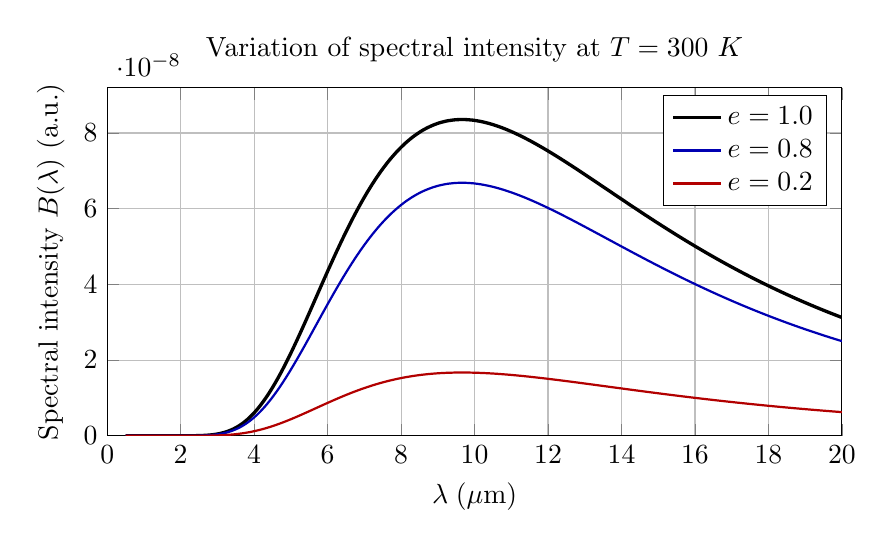
\begin{tikzpicture}
\begin{axis}[
  width=0.9\linewidth,
  height=6cm,
  xlabel={$\lambda\;(\mu\mathrm{m})$},
  ylabel={Spectral intensity $B(\lambda)$ (a.u.)},
  title={Variation of spectral intensity at $T=300\ \text{K}$},
  xmin=0, xmax=20,
  ymin=0,
  samples=300,
  domain=0.5:20,
  legend style={at={(0.98,0.98)},anchor=north east},
  grid=major,
  declare function={planck(\x)=(1/(\x^5))/(exp(47.959/\x)-1);} 
]
\addplot[black, very thick, smooth] {planck(x)};
\addlegendentry{$e=1.0$}
\addplot[blue!70!black, thick, smooth] {0.8*planck(x)};
\addlegendentry{$e=0.8$}
\addplot[red!70!black, thick, smooth] {0.2*planck(x)};
\addlegendentry{$e=0.2$}
\end{axis}
\end{tikzpicture}
\end{center}
The solar constant:
\[S\approx 1400\ \text{W\,m}^{-2}\]
(calculated using $I=\dfrac{P}{4\pi d^2}$, where $I$ is intensity, power of radiation received or emitted per unit area; $P=3.9\times 10^{26}\ \text{W}$ (total power the sun emitted), $d=1.5\times 10^{11}\ \text{m}=1$ au, average earth-sun distance)\\
It is the intensity of the solar radiation at the top of the earth's atmosphere.\\
The intensity emitted by the sun is
\[I=\dfrac{3.9\times 10^{26}\ \text{W}}{4\pi (7.0\times 10^8\ \text{m})^2}=6.3\times 10^7\ \text{W\,m}^{-2}\]
\subsection{Energy balance of the earth}
\begin{center}
  \begin{tikzpicture}

\def\sx{10.0}  % sphere center x
\def\sy{0}     % sphere center y
\def\sr{2.6}   % sphere radius

%── Left: 4 parallel yellow arrows (solar radiation) ──────────────
\foreach \y in {-1.5, -0.5, 0.5, 1.5} {
  \draw[-{Stealth[length=13pt, width=8pt]},
        line width=2.5pt, yellow!90!orange]
    (0, \y) -- (4.4, \y);
}
\node[below, align=center] at (2.2, -2.15)
  {solar radiation};

%── Middle: thick vertical disc line ──────────────────────────────
\draw[line width=7pt, black, line cap=round]
  (5.2, -2.6) -- (5.2, 2.6);
\node[below, align=center] at (5.2, -3.1)
  {disc of area $4\pi R^2$};

%── Right: sphere with radial green → blue gradient ────────────────
\shade[shading=axis, left color=green!65, right color=blue!85, shading angle=45r]
  (\sx, \sy) circle (\sr);
\draw[thick, black] (\sx, \sy) circle (\sr);

%── center dot ─────────────────────────────────────────────────────
\fill[white] (\sx, \sy) circle (3.5pt);

%── Dotted radius line from center to right edge ──────────────────
\draw[densely dotted, line width=1.4pt, white]
  (\sx, \sy) -- (\sx+\sr, \sy);

%── Radius label ───────────────────────────────────────────────────
\node[above, white] at (\sx+\sr/2, 0.12) {$R$};

%── Sphere surface-area label ──────────────────────────────────────
\node[below, align=center] at (\sx, \sy-\sr-0.7)
  {surface area of the sphere $4\pi R^2$};

\end{tikzpicture}
\end{center}
The radiation that reaches the earth has to go through the area of a disc of radius $R$ (the Earth's radius).\\
The power going through the disc is given by
\[P=S\pi R^2(=SA)\]
where $S$ is the solar constant, $A$ is the area of the disc.\\
The average intensity reaching the Earth's surface is 
\[I_\text{av}=(1-\alpha)\dfrac{S}{4}=245\ \text{W\,m}^{-2}\]
where $\alpha\approx 0.30$ (albedo of the earth varies and depends on (for example) the latitude and whether covered by clouds or not, here 0.3 is an average), and $\dfrac{S}{4}$ is found by diving the the power through the disc by the surface area of the earth.
\\\\Energy balance equation: (very simple, not considering greenhouse effect)
\[(1-\alpha)\dfrac{S}{4}=\sigma T^4\]
\subsubsection*{Greenhouse gases}
\begin{center}
  \begin{tikzpicture}[line cap=round, line join=round]

%% ─── Long thin rectangle: blue (top) → green (bottom) ───────────
\shade[top color=blue!70, bottom color=green!55]
  (-5.8, 0) rectangle (5.8, 0.52);
\draw[thick] (-5.8, 0) rectangle (5.8, 0.52);
\node[white, font=\scriptsize] at (0, 0.26)
  {received by the Earth and atmosphere};
\node[below, font=\small] at (0, -0.08)
  {Earth's surface};

%% ─── LEFT: incoming intensity ─────────────────────────────────────
%% Thick yellow arrow, perpendicular (straight down ↓) to rectangle
\draw[-{Stealth[length=13pt, width=10pt]},
      line width=3pt, yellow!85!orange]
  (-3.6, 4.5) -- (-3.6, 0.52);
\node[right, font=\scriptsize, align=left] at (-3.25, 2.5)
  {incoming\\intensity};

%% ─── LEFT: reflected ──────────────────────────────────────────────
%% Much thinner, shorter, forms an angle with incoming, pointing ↖
\draw[-{Stealth[length=7pt, width=4pt]},
      line width=2pt, yellow!85!orange]
  (-3.6, 0.52) -- (-5.1, 2.6);
\node[left, font=\scriptsize] at (-4.8, 1.55) {reflected};

%% ─── RIGHT: radiated back into space ──────────────────────────────
%% Relatively thick arrow pointing straight up ↑
\draw[-{Stealth[length=13pt, width=10pt]},
      line width=3pt, yellow!85!orange]
  (0.6, 0.52) -- (0.6, 5.0);
\node[right, font=\scriptsize, align=left] at (0.9, 4.5)
  {radiated back\\into space};

%% ─── RIGHT: U-turn (re-radiated greenhouse IR) ────────────────────
%% Rises from rectangle, arches over at ~mid-height, returns to rect
\draw[-{Stealth[length=10pt, width=8pt]},
      line width=2.8pt, yellow!85!orange]
  (0.6, 1)
  -- (0.6, 2.7)
  arc[start angle=180, end angle=0, radius=0.75]
  -- (2.1, 1.5);

%% Label inside U-turn area
\node[font=\scriptsize, align=center, text width=1.6cm] at (3.65, 2.5)
  {reabsorbed IR radiation re-radiated back to Earth};

%% ─── Dashed box around U-turn arrow + label ───────────────────────
\draw[dashed, thin, black] (0, 1) rectangle (5.2, 3.65);

%% "greenhouse effect" at the top of the dashed box
\node[right] at (3.5, 4.1)
  {\textit{greenhouse effect}};

\end{tikzpicture}
\end{center}
A thorough process of how did the greenhouse effect occur:
\begin{enumerate}
  \item Infrared radiation emitted from the Earth's surface is strongly absorbed by greenhouse gases in the atmosphere
  \item This radiation is in turn re-radiated by these gases in all directions.
  \item This means that some of this radiation is received by the earth's surface again, causing additional warming.
\end{enumerate}
Enhanced greenhouse effect:  additional warming due to increased quantities of the greenhouse gases in the atmosphere. The increases in the gas concentrations are due to human activity and are closely related to the burning of fossil fuels.
\begin{center}
  \begin{tabularx}{\textwidth}{@{}|Y |Y |Y|@{}}
\toprule
\textbf{Greenhouse gas} & \textbf{Natural sources} & \textbf{Anthropogenic sources}\\
\midrule
$H_2O$ & evaporation of water from oceans, rivers and lakes & irrigation \\\hline
$CO_2$ & forest fires, volcanic eruptions, evaporation of water from oceans & burning of fossil fuels, deforestation \\\hline
$CH_4$ & wetlands, ocean, lakes, rivers, termites & agriculture (rice cultivation), livestock farming, landfill sites \\\hline
$N_2O$ & oceans, forests, soils, tropical forests & agriculture (fertilizer use), burning of fossil fuels, munufacture of cement, deforestation (reduction of nitrogen fixation) \\
\bottomrule
\end{tabularx}
\end{center}
\begin{center}
  \begin{tikzpicture}[
    >=Latex,scale=0.8
]

\node[
    cloud,
    cloud puffs=14,
    cloud puff arc=120,
    draw=none,
    fill=gray!20,
    minimum width=6cm,
    minimum height=3cm,
    align=center
] (g) {greenhouse\\gases};
% Incoming radiation from Earth
\draw[
    red,
    fill=red
]
(-0.45,-4.2) -- (0.45,-4.2) --
(0.45,-2.4) --
(0.9,-2.4) --
(0,-1.5) --
(-0.9,-2.4) --
(-0.45,-2.4) -- cycle;

\node[align=center] at (0,-5.1)
{radiation from\\Earth's surface};

% Outgoing radiation
\draw[
    red,
    fill=red
]
(-0.45,2.4) -- (0.45,2.4) --
(0.45,4.2) --
(0.9,4.2) --
(0,5.1) --
(-0.9,4.2) --
(-0.45,4.2) -- cycle;

\node[align=center] at (0,6.0)
{radiation missing\\IR photons};

% Re-emitted IR photons
\foreach \ang in {0,60,120,180,240,300}
{
    \draw[
        red,
        very thick,
        ->,
        opacity=0.7
    ]
    ({1.6*cos(\ang)},{1.6*sin(\ang)})
    --
    ({3.1*cos(\ang)},{3.1*sin(\ang)});
}

\node[align=left] at (5.8,0)
{IR photons\\re-emitted in all\\directions};

\end{tikzpicture}
\end{center}
The energy of the molecules are \textbf{discrete}. The difference in energy between molecular energy levels is the energy of an infrared photon. 
\begin{itemize}
  \item Infrared photons travelling through greenhouse gases will be absorbed.
  \item The gas molecules that have absorbed the photons will now be excited to higher energy levels. 
  \item But the molecules prefer to be in low-energy states, and so they will immediately make a transition to a lower-energy state by emitting the photons they absorbed. 
  \item The emitted photons have the same energy as the absorbed photons, but they are emitted in random directions.
  \item Some are emitted back towards the earth, thereby warming the earth's surface.
\end{itemize} 
OR
\begin{itemize}
  \item \textbf{Resonance:} All systems have their own natural frequency of oscillation, and resonance happens when the frequency of the incoming radiation matches the natural frequency of the system.
  \item In the case of the greenhouse gases, the natural frequency is the frequency of the photons the greenhouse gases can absorb.
  \item Resonance is achieved when the photons emitted by the earth's surface have the same frequency as the natural frequency. (i.e., the energy of the photons emitted by the earth's surface is the same as the energy difference between the molecular energy levels of the greenhouse gases)
  \item Photons with the right energy (frequency) will be absorbed by the greenhouse gases, and then re-emitted in random directions, some of which will be back towards the earth's surface, causing additional warming.
\end{itemize}
\section{The gas laws}
\subsection{Moles, molar mass and the Avogadro constant}
I assume we have some IG chemistry memory coming back?\\
1 mole of any substance contains as many particles (atoms / molecules, depends) as atoms in 12 g of carbon-12.\\
$1 \text{ mol} = 6.02 \times 10^{23} \text{ particles}$\\
This is also known as the Avogadro constant, $N_A$.\\
$n=\dfrac{N}{N_A}$ if $n$ is the number of moles, $N$ is the number of particles.\\
The molar mass of a substance is the mass (in grams) of 1 mole of that substance.\\
$_Z^AX$ has approximately a molar mass of $A$ g/mol.\\
$n=\dfrac{m}{\mu}$, where $\mu$ is the molar mass, $m$ is the mass of the substance, $n$ is the number of moles.
\subsection{Ideal gases}
Pressure: the normal force applied per unit area. Commonly known as $P = \dfrac{F}{A}$, but as shown in the diagram below, the formula should be adjusted as $P=\dfrac{F\cos\theta}{A}$.
\begin{center}
      \begin{tikzpicture}[scale=0.9]
        % 3D side view: surface tilted to show depth
        % Surface (light yellow ellipse viewed at angle)
        \coordinate (O) at (0,0);
        \coordinate (SurfaceLeft) at (-2,0);
        \coordinate (SurfaceRight) at (2,0);
        \coordinate (SurfaceBack) at (-1.5,-1.5);
        

        % Draw circular contact area (as ellipse in 3D view)
        \draw[orange!70!black, thick, dashed] 
          (0,0) ellipse (2.4 and 0.8);
        \fill[yellow!60, opacity=0.5] 
          (0,0) ellipse (2.4 and 0.8);
        
        % Surface normal (dashed line)
        \draw[dashed, gray!70!black, thick] (0,0) -- (0,3);
        \node[label, below] at (0,3.5) {Normal};
        
        % Normal force (green arrow at angle θ)
        \draw[-{Latex[length=4mm]}, green!50!black, very thick, line width=1.5pt] 
          (-2.1,3) -- (0,0);
        \node[green!50!black, anchor=west] at (-2.2,3.2) {$N$};
        
        % Angle θ marking (between dashed normal and green force)
        \draw[gray!70!black] (0,0.5) arc[start angle=90, end angle=125, radius=0.5];
        \node[gray!70!black] at (-0.4,1.2) {$\theta$};
        
        % Labels
      \end{tikzpicture}
\end{center}
$1\ \text{atm}\approx 1.01\times 10^5\ \text{Pa}$\\\\
Lydia 丝滑连招解释压强（哎呀hào sí huà yā）:
\begin{center}
  \begin{tikzpicture}[scale=1.1]
    % Container wall (thin brown rectangle at bottom)
    \draw[fill=brown!40, draw=brown!70!black, very thick] (-3.5,-0.3) rectangle (3.5,0);
    \node[font=\small, below] at (0,-0.5) {Container wall};
    
    % Blue ball approaching from upper left at angle θ
    \fill[blue!60, draw=blue!80!black, thick] (-2.0, 2.2) circle (0.2);
    
    % Red arrow showing incoming path
    \draw[-{Latex[length=3mm]}, red!70!black, very thick] (-1.9, 2.1) -- (0, 0.3);
    
    % Angle θ from normal (vertical dashed line)
    \draw[dashed, gray!70!black, thick] (-2.0, 0) -- (-2.0, 1.8);
    \node[gray!70!black, font=\small] at (-1.8, 1.6) {$\theta$};
    
    % Blue ball rebounding to upper right at angle θ
    \fill[blue!60, draw=blue!80!black, thick] (2.0, 2.2) circle (0.2);
    
    % Red arrow showing outgoing path (reflected)
    \draw[-{Latex[length=3mm]}, red!70!black, very thick] (0.1, 0.3) -- (2, 2.1);
    \node[label, above] at (1, 1.2) {$v$};
  \end{tikzpicture}
\end{center}
\begin{itemize}
  \item $|\Delta \vec{p}|=2mv\cos\theta$
  \item This change of momentum means that there is a force acting on the wall in a short amount of time
  \item By Newton's third law, therefore, the molecule exerted on the wall an equal and opposite force.
  \item Taking into account the forces due to all the molecules colliding with the walls results in a force.
\end{itemize}
\subsubsection*{Ideal gas}
\begin{itemize}
  \item The molecules are point particles, each with negligible volume.
  \item The molecules obey the laws of mechanics.
  \item There are no forces between the molecules except when the molecules collide.
  \item The duration of a collision is negligible compared to the time between collisions.
  \item The collisions of the molecules with each other and with the container walls are elastic.
  \item Molecules have a range of speeds and move randomly.
  \item They can't be liquefied / solidified.
\end{itemize}
A real gas may be approximated by an ideal gas at low density which is equivalent to low pressure and moderate temperature.\\
The state of a gas is linked by $P$, $V$, $T$, and $n$ (number of moles).\\\\
How the ideal gas law is derived: (三巨头吓哭了)
\begin{itemize}
  \item Boyle's law: $PV=\text{constant}$ (at constant $T$ and $n$)
  \item Charles's law: $\dfrac{V}{T}=\text{constant}$ (at constant $P$ and $n$)
  \item Gay-Lussac's law: $\dfrac{P}{T}=\text{constant}$ (at constant $V$ and $n$)
\end{itemize}
Combining these three laws gives us the ideal gas law:
\[PV=nRT=k_BNT\]
$^*:$ Note that $n$ is the number of moles, $N$ is the number of particles, $R$ is the ideal gas constant, $R=8.31\ \text{J\,mol}^{-1}\,\text{K}^{-1}$, and $k_B$ is the Boltzmann constant, $k_B=\dfrac{R}{N_A}=1.38\times 10^{-23}\ \text{J\,K}^{-1}$.\\
In exam questions, use the equality $\dfrac{P_1V_1}{n_1T_1}=\dfrac{P_2V_2}{n_2T_2}$.
\begin{center}
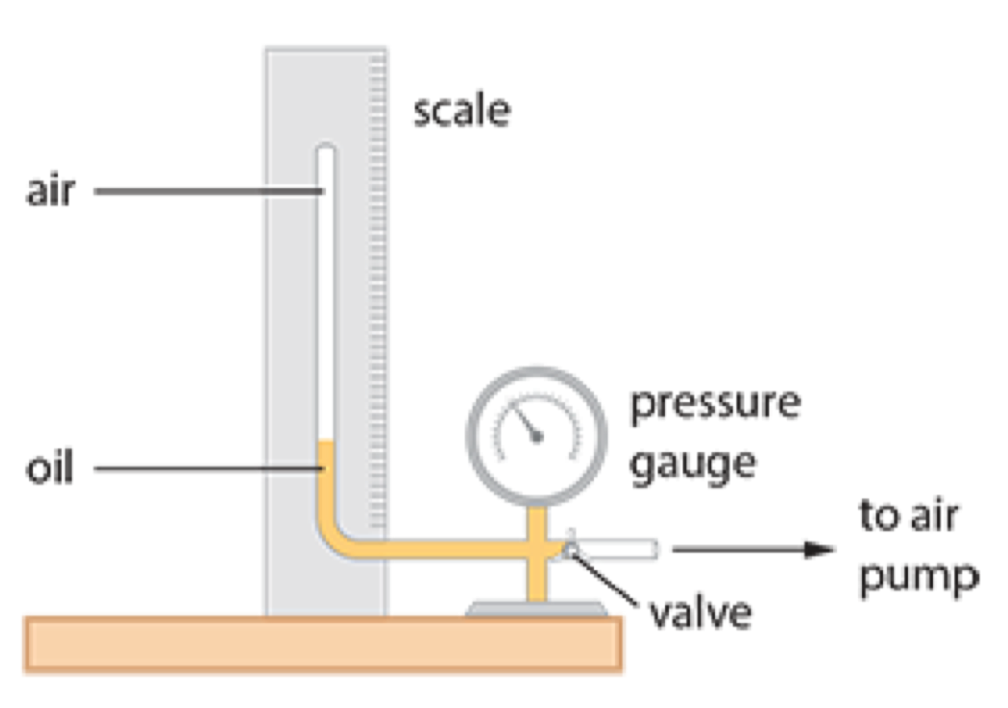
\includegraphics[width=0.3\linewidth]{截圖 2026-06-02 23.01.21.png}
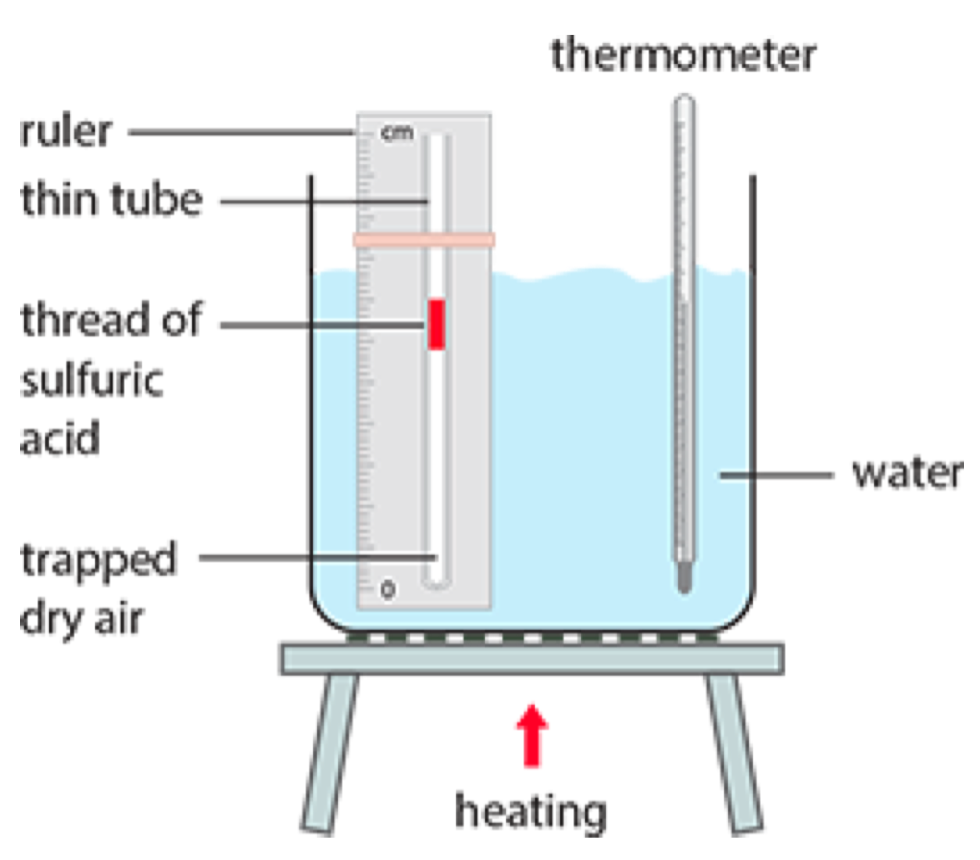
\includegraphics[width=0.3\linewidth]{截圖 2026-06-02 23.01.31.png}
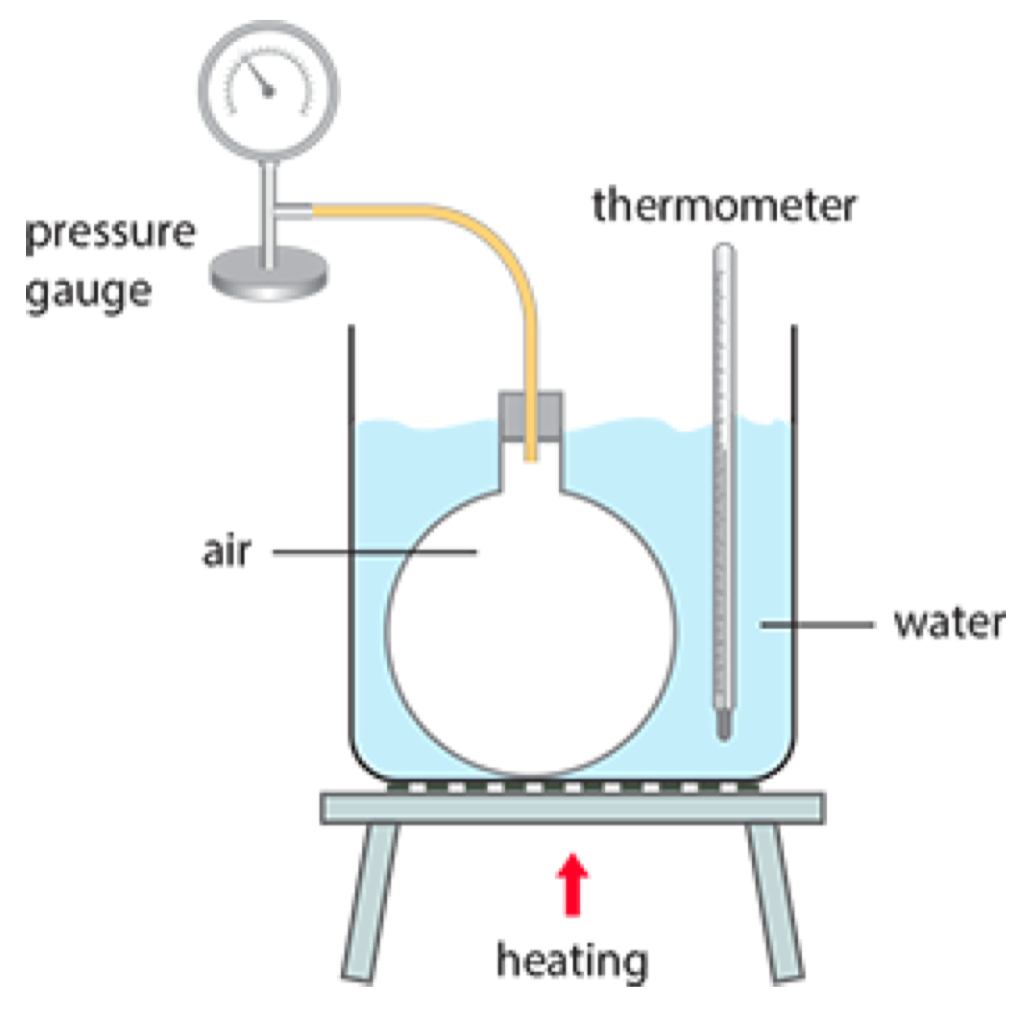
\includegraphics[width=0.3\linewidth]{截圖 2026-06-02 23.01.41.png}
\end{center}
\subsection{The Boltzmann equation}
The molecules of a gas move about randomly with a range of speeds. The speed at the peak represents the most probable speed that would be found if you picked a molecule at random.
\begin{center}
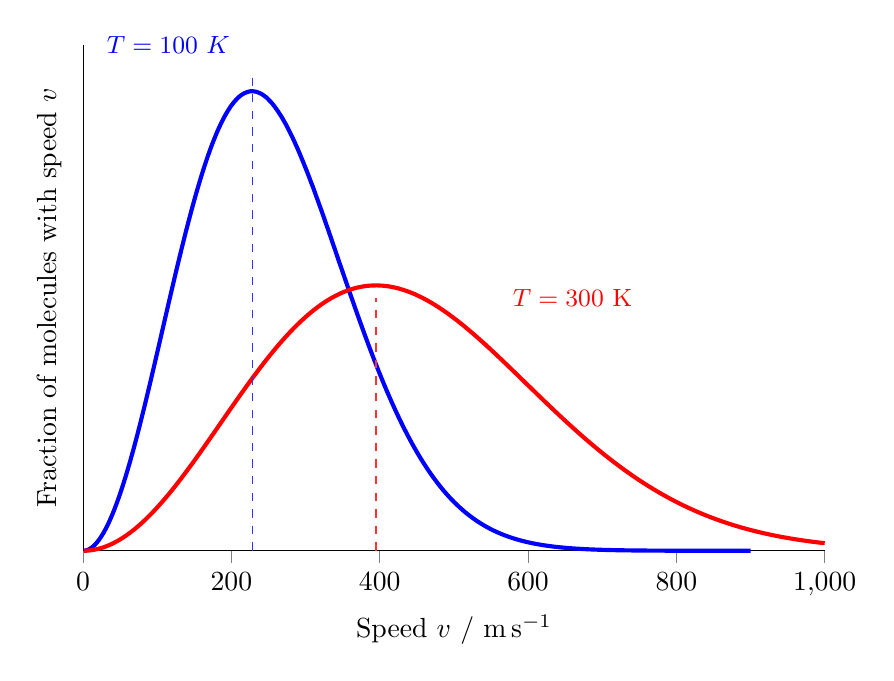
\begin{tikzpicture}
\begin{axis}[
  width=11cm,
  height=8cm,
  xlabel={Speed $v$ / m\,s$^{-1}$},
  ylabel={Fraction of molecules with speed $v$},
  xmin=0, xmax=1000,
  ymin=0, ymax=0.004,
  xtick={0,200,400,600,800,1000},
  ytick=\empty,
  axis lines=left,
  axis line style={-},
  tick align=outside,
  clip=false,
]

%--- Blue curve: O2 at T = 100 K ---
% Maxwell--Boltzmann: f(v) = 4*pi*(M/2piRT)^{3/2} * v^2 * exp(-Mv^2/2RT)
% M = 0.032 kg/mol, R = 8.314 J/(mol K)
% Prefactor A = 4*pi*(M/2piRT)^{3/2} = 1.902e-7
% Exponent coefficient b = M/(2RT) = 1.924e-5
% Most probable speed: v_p = sqrt(2RT/M) = 228 m/s
\addplot[blue, line width=1.5pt, domain=1:900, samples=400, smooth]
  {1.902e-7 * x^2 * exp(-1.924e-5 * x^2)};

%--- Red curve: O2 at T = 300 K ---
% Prefactor A = 3.661e-8
% Exponent coefficient b = M/(2RT) = 6.413e-6
% Most probable speed: v_p = sqrt(2RT/M) = 395 m/s
\addplot[red, line width=1.5pt, domain=1:1000, samples=400, smooth]
  {3.661e-8 * x^2 * exp(-6.413e-6 * x^2)};

% Dashed vertical lines marking the most probable speeds
\draw[blue!80, dashed, thin] (axis cs:228, 0) -- (axis cs:228, 0.00375);
\draw[red!80,  dashed, thin] (axis cs:395, 0) -- (axis cs:395, 0.002);

% Curve labels
\node[blue, font=\small] at (axis cs:115, 0.004) {$T = 100\ \text{K}$};
\node[red,  font=\small] at (axis cs:660, 0.002) {$T = 300\ \mathrm{K}$};

\end{axis}
\end{tikzpicture}
\end{center}
The root mean square speed of the molecules is given by
\[c=\sqrt{\dfrac{\sum_{i=1}^{n}v_i^2}{N}}\]
The average kinetic energy of the molecules is given by
\[\overline{E}_k = \dfrac{1}{2}mc^2\]
where $m$ is the mass of a molecule, $c$ is the root mean square speed of the molecules.\\
Note that we will use $c$ to represent the root mean square speed, most probable speed, and the average speed.\\
The equation for the pressure of the gas is given by
\[P=\dfrac{1}{3}\rho c^2\]
下面是推导过程（考试不需要）:\\
$\vec{J}=2mv_x\ (\text{a molecule with mass $m$ and velocity $v_x$ collides with the wall and rebounds})$\\
$T=2\dfrac{L}{v}\ (\text{time between collisions on the right side of the wall, assume the length of the container is $L$})$\\
$\dfrac{J}{T}=\dfrac{2mv_x}{2\dfrac{L}{v}}=\dfrac{mv_x^2}{L}\ (\text{average force exerted by the molecule on the wall over large amount of time})$\\
$P_\text{molecule}=\dfrac{mv_x^2}{L^3}=\dfrac{mv_x^2}{V}\ (\text{pressure exerted by the molecule on the wall, container is a cube})$\\
$\displaystyle P_\text{total}=\dfrac{m}{V}\sum_{i=1}^{N}v_{x,i}^2\ (\text{pressure exerted by all the molecules on the wall})$\\
$\overline{v_x^2}=\dfrac{\sum_{i=1}^{N}v_{x,i}^2}{N}\ (\text{average of $v_x^2$}) \Rightarrow P=\dfrac{mN}{V}\overline{v_x^2}$\\
$\because \overline{v_x^2}=\overline{v_y^2}=\overline{v_z^2}\text{ and } \overline{v_x^2}+\overline{v_y^2}+\overline{v_z^2}=c^2 \therefore \overline{v_x^2}=\dfrac{c^2}{3} \Rightarrow P=\dfrac{1}{3}\dfrac{mN}{V}c^2=\dfrac{1}{3}\rho c^2$\\
The average kinetic energy of the molecules is also given by
\[ \overline{E}_k = \dfrac{3}{2}k_BT\]
where $k_B$ is the Boltzmann constant, $T$ is the absolute temperature of the gas.\\
This exceptional equation relates a microscopic quantity, the average kinetic energy of molecules, to a macroscopic quantity, temperature. It also says that at $T = 0$, all molecular motion stops.\\\\
The total internal energy of an ideal gas (i.e. total random kinetic energy) is given by
\[U=\dfrac{3}{2}Nk_BT=\dfrac{3}{2}nRT=\dfrac{3}{2}PV\]
\section{Thermodynamics}
\subsection{Internal energy}
The change in internal energy: (ideal gas)
\[\Delta U=\dfrac{3}{2}Nk_B\Delta T=\dfrac{3}{2}nR\Delta T=\dfrac{3}{2}P\Delta V=\dfrac{3}{2}V\Delta P\]
\begin{center}
\begin{tikzpicture}[font=\small]

%------------------------------------------------------------
% Panel (a): T_sys < T_surr  →  heat enters the system
%------------------------------------------------------------
\begin{scope}[xshift=0cm]

  % Surroundings (warmer → orange tint)
  \fill[orange!25] (-3.2,-2.6) rectangle (3.2,2.6);
  \draw[thick]     (-3.2,-2.6) rectangle (3.2,2.6);

  % System (cooler → blue tint)
  \fill[cyan!40]   (-1.3,-1.1) rectangle (1.3,1.1);
  \draw[thick]     (-1.3,-1.1) rectangle (1.3,1.1);

  % Labels
  \node[font=\small\bfseries]  at (0,  0.42) {System};
  \node[font=\footnotesize]    at (0, -0.08) {$T_{\mathrm{sys}}$ (lower)};

  % Wavy heat arrow entering from left
  \draw[-{Stealth[length=9pt, width=7pt]}, ultra thick, red!80!black,
        decorate,
        decoration={snake, amplitude=2.5pt, segment length=8pt, post length=9pt}]
      (-3.2, 0) -- (-1.3, 0);
  \node[red!80!black, above] at (-2.25, 0.15) {$Q$};

  % Wavy heat arrow entering from top
  \draw[-{Stealth[length=9pt, width=7pt]}, ultra thick, red!80!black,
        decorate,
        decoration={snake, amplitude=2.5pt, segment length=8pt, post length=9pt}]
      (0, 2.6) -- (0, 1.1);
  \node[red!80!black, right] at (0.12, 1.85) {$Q$};

  % Wavy heat arrow entering from right
  \draw[-{Stealth[length=9pt, width=7pt]}, ultra thick, red!80!black,
        decorate,
        decoration={snake, amplitude=2.5pt, segment length=8pt, post length=9pt}]
      (3.2, 0) -- (1.3, 0);
  \node[red!80!black, above] at (2.25, 0.15) {$Q$};

  % Panel label
  \node[font=\bfseries] at (-2.85, 2.35) {(a)};

  % Caption
  \node[align=center] at (0,-3.35)
    {$T_{\mathrm{sys}} < T_{\mathrm{surr}}$\\[2pt]Heat \textit{enters} the system};

\end{scope}

%------------------------------------------------------------
% Panel (b): T_sys > T_surr  →  heat leaves the system
%------------------------------------------------------------
\begin{scope}[xshift=8cm]

  % Surroundings (cooler → blue tint)
  \fill[cyan!18]   (-3.2,-2.6) rectangle (3.2,2.6);
  \draw[thick]     (-3.2,-2.6) rectangle (3.2,2.6);

  % System (warmer → orange tint)
  \fill[orange!50] (-1.3,-1.1) rectangle (1.3,1.1);
  \draw[thick]     (-1.3,-1.1) rectangle (1.3,1.1);

  % Labels
  \node[font=\small\bfseries]  at (0,  0.42) {System};
  \node[font=\footnotesize]    at (0, -0.08) {$T_{\mathrm{sys}}$ (higher)};

  % Wavy heat arrow leaving to the left
  \draw[-{Stealth[length=9pt, width=7pt]}, ultra thick, red!80!black,
        decorate,
        decoration={snake, amplitude=2.5pt, segment length=8pt, post length=9pt}]
      (-1.3, 0) -- (-3.2, 0);
  \node[red!80!black, above] at (-2.25, 0.15) {$Q$};

  % Wavy heat arrow leaving to the top
  \draw[-{Stealth[length=9pt, width=7pt]}, ultra thick, red!80!black,
        decorate,
        decoration={snake, amplitude=2.5pt, segment length=8pt, post length=9pt}]
      (0, 1.1) -- (0, 2.6);
  \node[red!80!black, right] at (0.12, 1.85) {$Q$};

  % Wavy heat arrow leaving to the right
  \draw[-{Stealth[length=9pt, width=7pt]}, ultra thick, red!80!black,
        decorate,
        decoration={snake, amplitude=2.5pt, segment length=8pt, post length=9pt}]
      (1.3, 0) -- (3.2, 0);
  \node[red!80!black, above] at (2.25, 0.15) {$Q$};

  % Panel label
  \node[font=\bfseries] at (-2.85, 2.35) {(b)};

  % Caption
  \node[align=center] at (0,-3.35)
    {$T_{\mathrm{sys}} > T_{\mathrm{surr}}$\\[2pt]Heat \textit{leaves} the system};

\end{scope}

\end{tikzpicture}
\end{center}
Concepts regarding \textit{systems}:
\begin{itemize}
  \item Systems: the complete set of objects under consideration
  \item Closed system: a system that can exchange energy but not matter with its surroundings, mass can not enter or leave the system.
  \item Isolated system: a system that can exchange neither energy nor matter with its surroundings
  \item If all the parameters defining the system are given, we speak of the system being in a particular state
  \item Any process that changes the state of a system is called a thermodynamic process
\end{itemize}
Internal energy is a property of the particular state of the system under consideration and therefore is a state function.Heat and work are related to changes in the state of the
system, not to the state itself.
\begin{center}
\begin{tabularx}{\textwidth}{@{}|Y |Y |Y|@{}}
\toprule
\textbf{Process} & \textbf{Description} & \textbf{Equation} \\
\midrule
Isothermal & Temperature is constant & \(P_1V_1=P_2V_2\) \\\hline
Isobaric & Pressure is constant & \(\dfrac{V_1}{T_1}=\dfrac{V_2}{T_2}\) \\\hline
Isovolumetric & Volume is constant & \(\dfrac{P_1}{T_1}=\dfrac{P_2}{T_2}\) \\\hline
Adiabatic & No heat exchange & \(P_1V_1^{\gamma}=P_2V_2^{\gamma}\), $\gamma=\dfrac{5}{3}$ \\
 & & \(T_1V_1^{\gamma-1}=T_2V_2^{\gamma-1}\), $\gamma-1=\dfrac{2}{3}$\\
\bottomrule
\end{tabularx}
\end{center}
Work done on / by the gas:
\[W=F\Delta s=PA\Delta s=P\Delta V\]
\begin{center}
  \begin{tikzpicture}[>=Stealth, line cap=round, line join=round]

%% ─── Geometry ──────────────────────────────────────────────────
\def\yt{ 0.85}   % bore top y
\def\yb{-0.85}   % bore bottom y
\def\wt{ 0.35}   % wall thickness
\def\piL{4.2}    % piston initial left face (x)
\def\piR{4.85}   % piston initial right face (x)
\def\ds{0.65}    % small compression δs

%% ─── Gas fill (initial state) ─────────────────────────────────
\fill[cyan!20] (0,\yb) rectangle (\piL,\yt);

%% ─── Left end wall ─────────────────────────────────────────────
\fill[gray!30] ({-\wt},{\yb-\wt}) rectangle (0,{\yt+\wt});
\path[pattern=north west lines, pattern color=gray!65]
     ({-\wt},{\yb-\wt}) rectangle (0,{\yt+\wt});

%% ─── Top wall ──────────────────────────────────────────────────
\fill[gray!30] (0,\yt) rectangle (5.8,{\yt+\wt});
\path[pattern=north west lines, pattern color=gray!65]
     (0,\yt) rectangle (5.8,{\yt+\wt});

%% ─── Bottom wall ───────────────────────────────────────────────
\fill[gray!30] (0,{\yb-\wt}) rectangle (5.8,\yb);
\path[pattern=north west lines, pattern color=gray!65]
     (0,{\yb-\wt}) rectangle (5.8,\yb);

%% ─── Bore outline ──────────────────────────────────────────────
\draw[thick] (0,\yt)  -- (5.8,\yt);   % top inner edge
\draw[thick] (0,\yb)  -- (5.8,\yb);   % bottom inner edge
\draw[thick] (0,\yb)  -- (0,\yt);     % left inner face

%% ─── Piston — initial position (solid) ────────────────────────
\fill[gray!65] (\piL,\yb) rectangle (\piR,\yt);
\draw[thick]   (\piL,\yb) rectangle (\piR,\yt);

%% ─── Piston — after δs compression (dashed) ──────────────────
\pgfmathsetmacro{\pL}{\piL-\ds}   % = 3.55  (new left face)
\pgfmathsetmacro{\pR}{\piR-\ds}   % = 4.20  (new right face = old left face)
\draw[dashed, thick, gray!70] (\pL,\yb) rectangle (\pR,\yt);

%% ─── δs dimension arrow (below bore) ──────────────────────────
\pgfmathsetmacro{\yArr}{\yb-0.48}
\draw[{Stealth[length=5pt,width=4pt]}-{Stealth[length=5pt,width=4pt]}, thin]
     (\pL,\yArr) -- (\piL,\yArr);
\node[below, font=\small] at ({(\pL+\piL)/2},{\yArr-0.05}) {$\delta s$};
% projection lines
\draw[thin, gray!55] (\pL ,\yb) -- (\pL ,{\yArr-0.12});
\draw[thin, gray!55] (\piL,\yb) -- (\piL,{\yArr-0.12});

%% ─── Gas pressure force on piston (outward arrow, blue) ───────
\draw[-{Stealth[length=9pt, width=6pt]}, thick, blue!70!black]
     (\piL,0) -- ({\piL+0.9},0);
\node[above, blue!70!black, font=\small] at ({\piL+0.35},0.08) {$PA$};

%% ─── External applied force (inward arrow, red) ───────────────
\draw[-{Stealth[length=11pt, width=8pt]}, ultra thick, red!80!black]
     (6.8,0) -- (\piR,0);
\node[above, red!80!black, font=\normalsize] at (5.85,0.1) {$F$};

%% ─── Labels ────────────────────────────────────────────────────
\node[font=\large\itshape] at (2.0, 0.28)              {gas};
\node[font=\small]          at (2.0,-0.24)             {pressure $p$};

% piston label with arrow
\node[font=\small] (plabel) at ({(\piL+\piR)/2}, 1.6) {piston};
\draw[->, thin] (plabel.south) -- ({(\piL+\piR)/2}, {\yt+\wt+0.05});

% dashed-piston annotation
\node[font=\footnotesize, gray!80, align=center]
     at ({\pL+0.4}, {-2.3}) {(after\\[-2pt]compression)};

\end{tikzpicture}
\end{center}
It could also be calculated by finding the area under the curve in a $P$-$V$ graph. (when pressure is not constant)
\begin{center}
  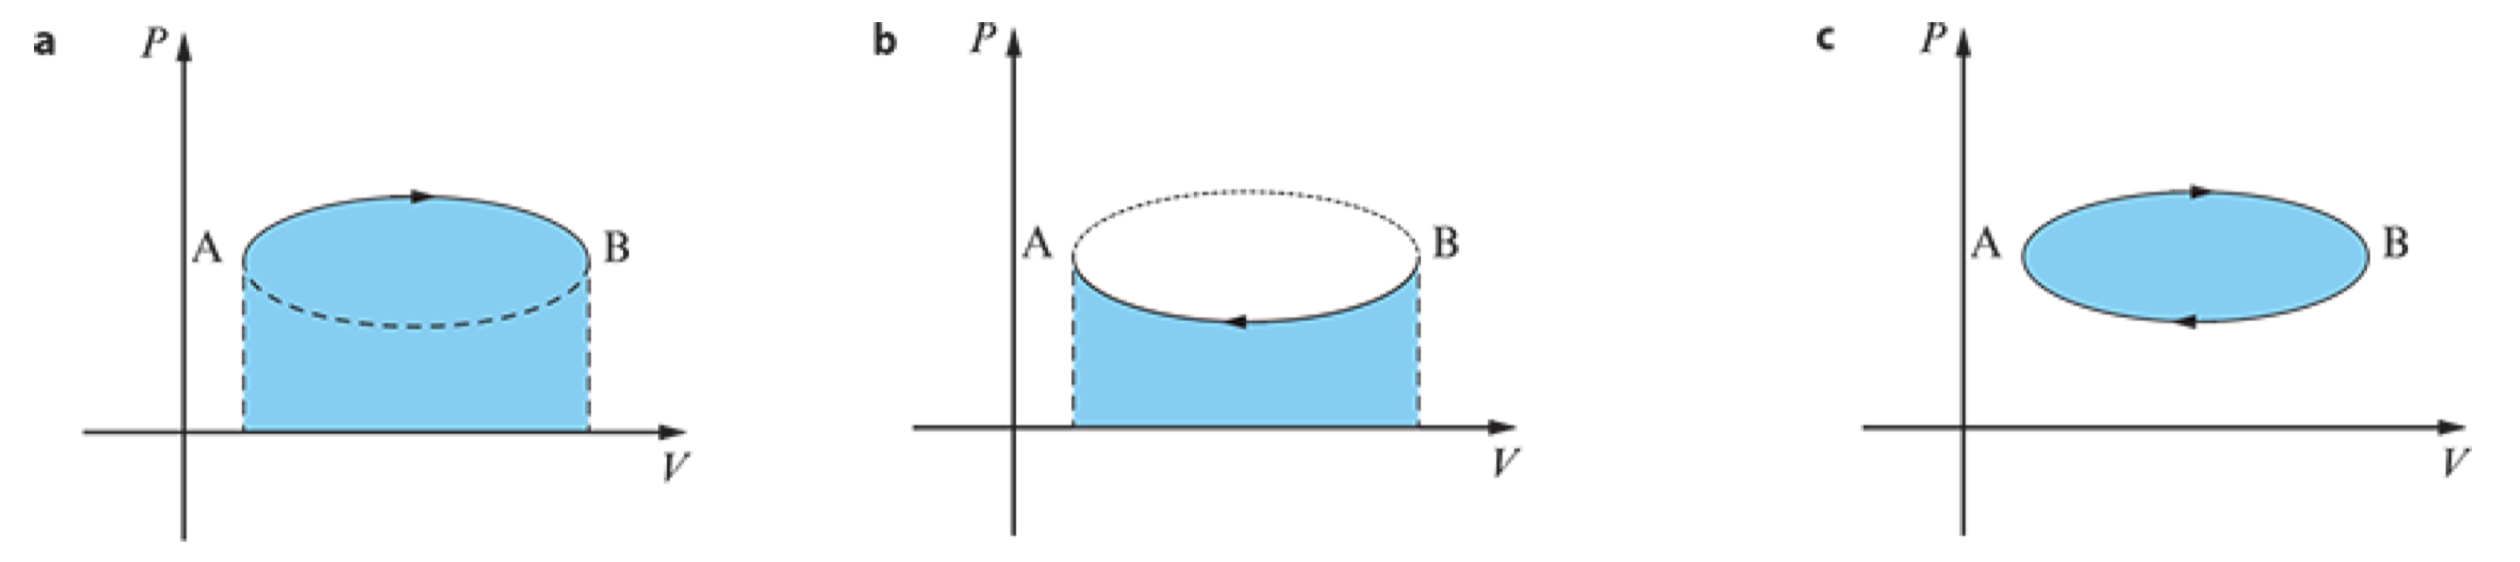
\includegraphics[width=0.9\linewidth]{截圖 2026-06-03 19.19.33.png}\\
  For a closed loop in a pressure-volume diagram, the work done is the area of the loop.\\
  (Work done expanding is shown in a, work done compressing is shown in b)\\
\end{center}
\subsection{The first law of thermodynamics}
The first law is just the law of conservation of energy applied to thermodynamics.
\[\underbrace{Q}_\text{heat}=\underbrace{\Delta U}_\text{change in internal energy}+\underbrace{W}_\text{work done}\]
\begin{itemize}
  \item $Q>0:$ heat is supplied to the system; $Q<0$: heat is removed from the system
  \item $\Delta U>0:$ internal energy / temperature increases; $\Delta U<0:$ internal energy / temperature decreases
  \item $W>0:$ work is done by the system (gas expands); $W<0:$ work is done on the system (gas compressed)
\end{itemize}
\subsection{The second law of thermodynamics}
克劳德·香农（Claude Shannon）说过：”熵是信息的度量。”永远的现代信息学之父，致敬。\\
It is quite extraordinary that this formula of thermodynamics has featured extensively in Claude Shannon's theory of information, a crucial part of modern telecommunications theory.

Entropy: a measure of the disorder of a system, or the number of ways the system can be arranged.\\
The change in entropy is given by
\[\Delta S = \dfrac{Q}{T}\]
where $Q$ is the quantity of heat given to or removed from the system at a temperature $T$ (in K).\\
\begin{itemize}
  \item When heat is supplied to the system, $Q>0$, $\Delta S>0$, the entropy of the system increases.
  \item When heat is removed from the system, $Q<0$, $\Delta S<0$, the entropy of the system decreases.
\end{itemize} 
For a reversible process that returns the system to its original state, the total change in entropy is zero (an example is the isothermal expansion / compression of gas).\\
Extension: \(\displaystyle \Delta S = \int \frac{dQ}{T}\) when the temperature is not constant.\\\\
The entropy of an isolated system never decreases. Entropy increases in realistic irreversible processes and stays the same in theoretical, idealized, reversible processes.
\begin{center}
  \begin{tikzpicture}[scale=0.6]

% =========================
% Figure (a)
% =========================

\node[font=\bfseries] at (0,3.6) {a};

\node at (1.5,3.6) {hot};
\node at (4.5,3.6) {cold};

\fill[red!70!orange] (0.5,1.2) rectangle (3.5,3.2);
\fill[blue!60!cyan] (3.5,1.2) rectangle (6.5,3.2);

\draw[gray!70,line width=6pt]
(-0.4,0.8) -- (9.4,0.8);

\draw[
    fill=black,
    draw=black,
    line width=1.5pt,
    -{Triangle[length=12pt,width=12pt]}
]
(2.0,2.2) -- (5.0,2.2);

\node[anchor=west] at (-0.4,0.15)
{here entropy increases};

% =========================
% Figure (b)
% =========================

\begin{scope}[xshift=11cm]

\node[font=\bfseries] at (0,3.6) {b};

\node at (1.5,3.6) {hot};
\node at (4.5,3.6) {cold};

\fill[red!70!orange] (0.5,1.2) rectangle (3.5,3.2);
\fill[blue!60!cyan] (3.5,1.2) rectangle (6.5,3.2);

\draw[gray!70,line width=6pt]
(-0.4,0.8) -- (9.8,0.8);

\draw[
    fill=black,
    draw=black,
    line width=1.5pt,
    -{Triangle[length=12pt,width=12pt]}
]
(5.0,2.2) -- (2.0,2.2);

\node[anchor=west,align=left] at (-0.4,-0.2)
{here entropy decreases--hence\\
this process does not happen};

\end{scope}

\end{tikzpicture}
\end{center}
We denote $\Omega (H)$ the number of microstates that correspond to a macrostate H. (for example, the possible arrangements of $N$ coins consisting of $H$ heads)\\
Entropy is defined as:
\[S=k_B\ln\Omega\]
where $\Omega$ is the number of microstates that correspond to the macrostate (e.g. total energy of the gas) of the system.\\
We see that the states which are likely to occur have large entropy.
\subsection{Heat engines}
Definition: a device that transfers thermal energy to mechanical or electrical energy, which can then be used to do mechanical work.
\begin{center}
  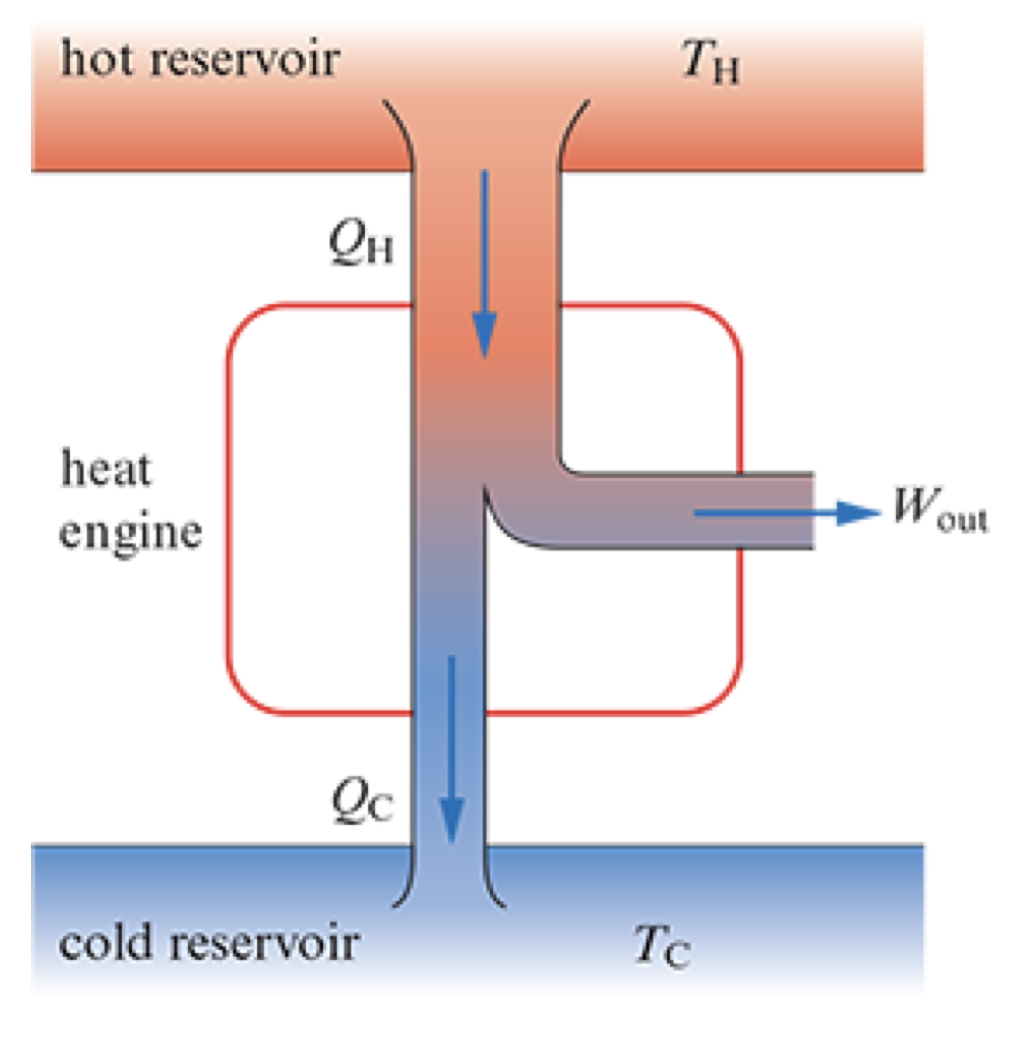
\includegraphics[width=0.25\linewidth]{截圖 2026-06-03 20.16.22.png}
  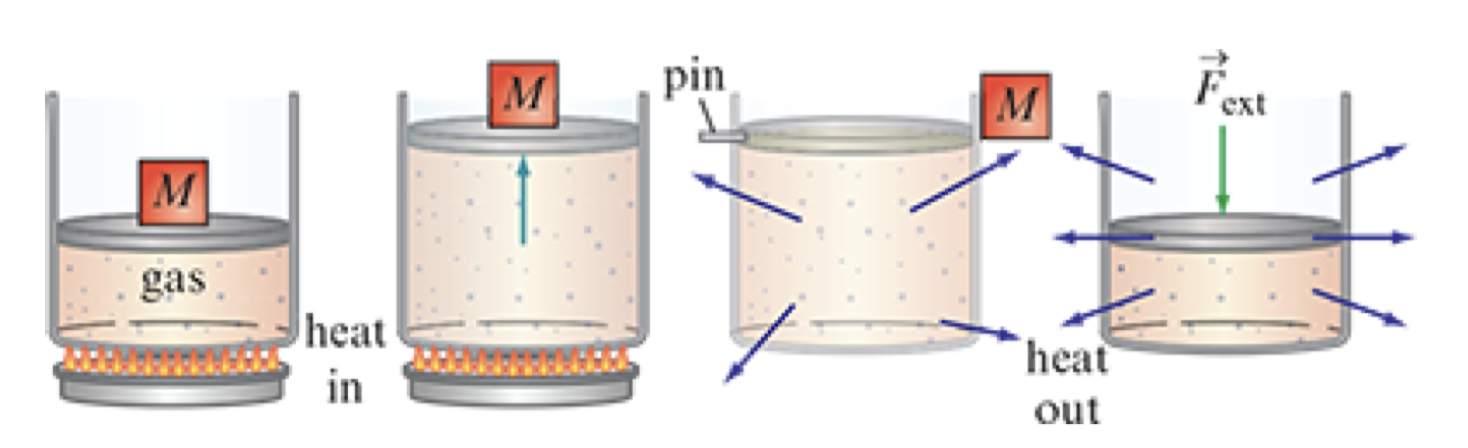
\includegraphics[width=0.74\linewidth]{截圖 2026-06-03 21.01.26.png}
\end{center}
\begin{itemize}
  \item A hot reservoir at temperature $T_H$ transfers heat $Q_H$ to the engine.
  \item The gas is expanded by the heat, doing work $W$ on the surroundings (in this case raising a load).
  \item Gas is allowed to cool down to a lower temperature $T_C$ isovolumetrically by transferring heat $Q_C$ to the cold reservoir (the surroundings).
  \item An external force compresses the gas isothermally back to the original state.
\end{itemize}
The efficiency of a heat engine:
\[\eta = \dfrac{\text{useful energy output}}{\text{energy input}}=\dfrac{W}{Q_h} = 1 - \dfrac{Q_c}{Q_h}\]
where $Q_h$ is the heat absorbed from the hot reservoir, $Q_c$ is the heat rejected to the cold reservoir, and $W$ is the work done by the engine. This shows that it is impossible to have a heat engine with 100\% efficiency.\\
\subsubsection*{Carnot cycle: limit on the efficiency of heat engines}
\begin{center}
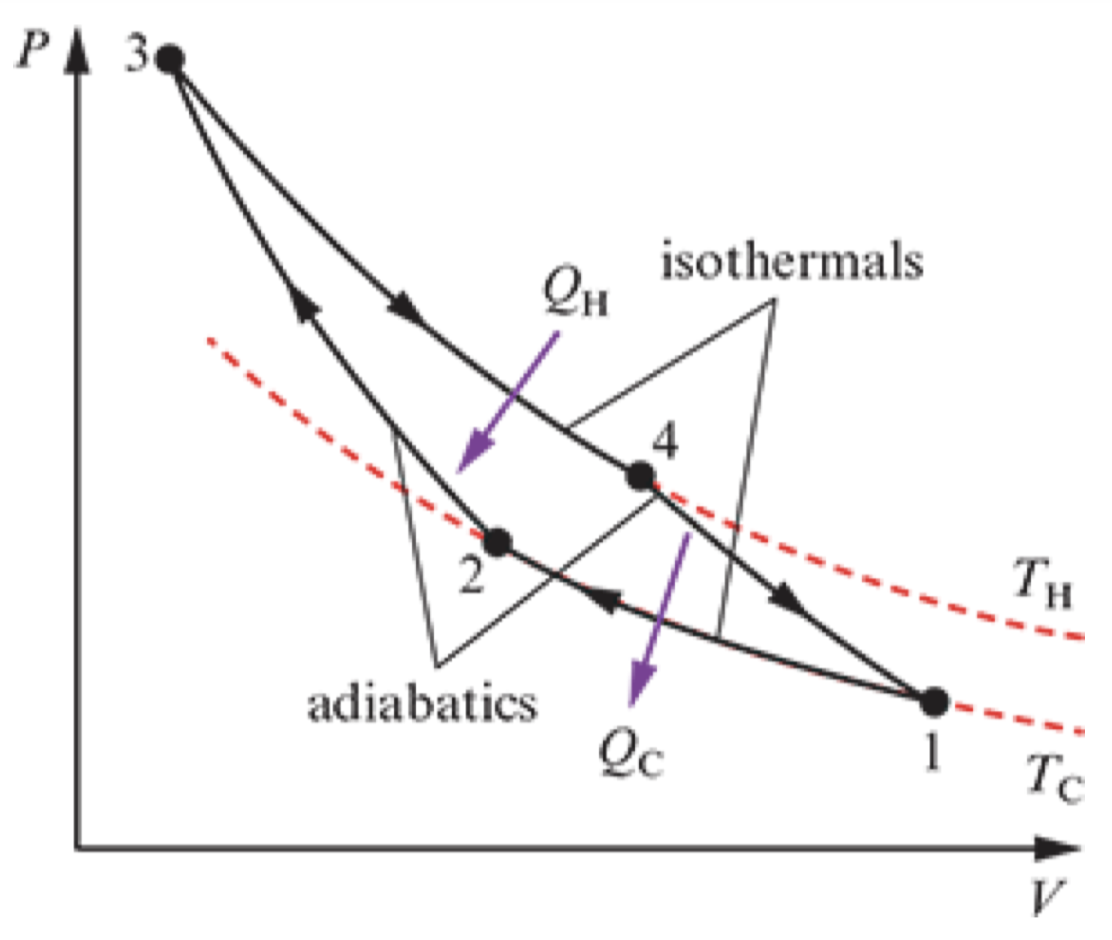
\includegraphics[width=0.4\linewidth]{截圖 2026-06-03 21.14.08.png}
\end{center}
\begin{itemize}
  \item The engine starts its cycle at 1.
  \item The gas is compressed isothermally until 2. During this stage heat $Q_C$ leaves the gas and work is done on the gas.
  \item From 2 to 3 it is compressed adiabatically; work is again done on the gas.
  \item From 3 to 4 the gas expands isothermally receiving heat $Q_H$ from a hot reservoir; work is done by the gas.
  \item From 4 to 1 the gas expands adiabatically; work is done by the gas.
\end{itemize}
The net work done by the engine is $W_\text{net}=Q_H-Q_C$\\
The change in entropy is $\Delta S=\Delta S_{1\to 2}+\Delta S_{2\to 3}+\Delta S_{3\to 4}+\Delta S_{4\to 1}$\\
$\Delta S_{3\to 4}=\dfrac{Q_H}{T_H}$, $\Delta S_{1\to 2}=\dfrac{Q_C}{T_C}$, $\Delta S_{2\to 3}=\Delta S_{4\to 1}=0$ (adiabatic, no heat exchange)\\
$\because \Delta S=0 \therefore \dfrac{Q_H}{T_H}=\dfrac{Q_C}{T_C}$\\
$\because \dfrac{Q_C}{Q_H}=\dfrac{T_C}{T_H} \therefore \eta = 1 - \dfrac{T_C}{T_H}$\\
This shows that the efficiency of a Carnot engine can never be 100\% because $T_C\neq 0$ and $T_H \neq \infty$.\\
\subsubsection*{Extension: proof of the Carnot efficiency being the maximum efficiency by contradiction}
\begin{center}
  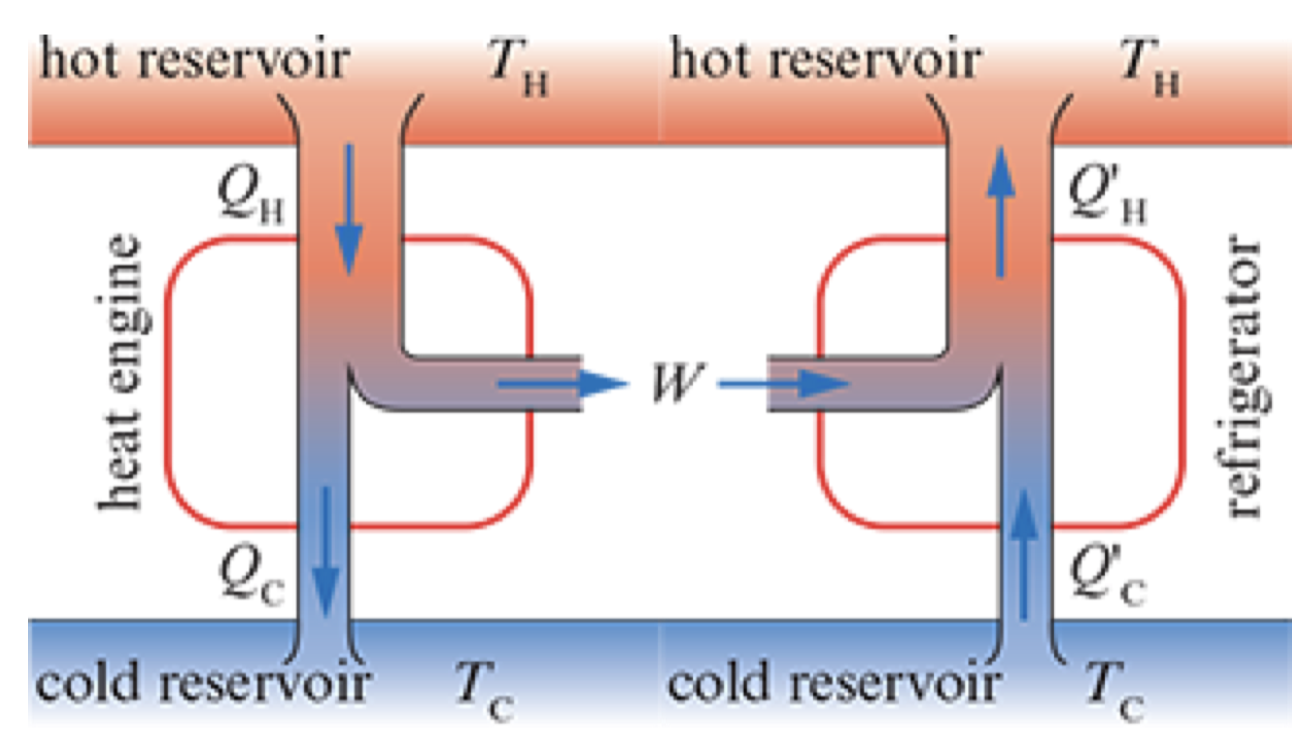
\includegraphics[width=0.5\linewidth]{截圖 2026-06-04 08.00.07.png}
\end{center}
If the Carnot refrigerator ran as a heat engine, the efficiency would be $\dfrac{W}{Q'_H}$.\\
If we assume the engine on the left has higher efficiency than the Carnot efficiency, then $\dfrac{W}{Q_H}>\dfrac{W}{Q'_H}$.\\
$\Rightarrow Q'_H>Q_H \Rightarrow Q'_H-Q_H>0$\\
$\because W=Q'_H-Q'_C=Q_H-Q_C \therefore Q'_C-Q_C=Q'_H-Q_H=Q>0$\\
The combination has the effect of transferring heat from the cold to the hot reservoir without performance of work, which is against the second law.\\
So the assumption of an engine with better efficiency than the Carnot efficiency must be false.
\section{Current and circuits}
\subsection{Potential difference, current and resistance}
$$V=\dfrac{W}{q}$$
where $W$ is the work done to move a charge $q$ through the component.\\
The kinetic energy gained when the charge is released (electric force will push it away) is $qV$.\\\\
Conductors: materials that allow electric charge to flow through them easily, many free electrons per unit volume. (for metals, $10^{28}$ free electron per cubic meter at $v$ of $10^5\ \text{m/s}$)\\
Insulators: materials that do not allow electric charge to flow through them easily, few or no free electrons per unit volume.\\
DC: direct current, the current flows / motion of electrons in one direction only.\\
AC: alternating current, the current / motion of electrons changes direction periodically.\\
$$I=\dfrac{\Delta q}{\Delta t}$$
$$R=\dfrac{V}{I}$$
Ohm's law: $I\propto V$ when temperature and $R$ are constant for ohmic conductors.\\
The resistance of a wire is given by
\[R=\rho\dfrac{L}{A}\]
where $\rho$ is the resistivity of the material, $L$ is the length of the wire, and $A$ is the cross-sectional area of the wire.\\\\
LDR: light dependent resistor, the resistance decreases as the intensity of light increases.\\
NTC Thermistor: the resistance decreases as the temperature increases.\\
Interpreting resistance at a microscopic level: 
\begin{itemize}
  \item Electrons suffer collisions with the atoms of the wire
  \item Collisions are inelastic, the electrons lose kinetic energy to the atoms, which causes the wire to heat up ($\uparrow \text{random }E_K \Rightarrow \uparrow T$)
  \item Atoms in the conductor vibrate more means an increased probability of collisions
  \item This reduces the speed of the electrons and therefore reduces the current, which is equivalent to an increase in resistance.
\end{itemize}
\subsection{Voltage, power and e.m.f}
\[V=IR\]
\[\text{electric power: } P=\dfrac{W}{\Delta t}=\dfrac{\Delta qV}{\Delta t} = IV=RI^2=\dfrac{V^2}{R}\]
This formula could also be used to calculate the power dissipated by a wire / electrical appliance.\\\\
Note that the conventional current is defined as flowing from positive to negative, which is opposite to the actual flow of electrons.\\
The electromotive force ($e.m.f$) $\varepsilon$ is the work done per unit charge by a source of electrical energy (e.g. battery) in moving a charge around a complete circuit.
\[\varepsilon = \dfrac{W}{q}=\dfrac{P}{I}\]
\subsection{Resistors in electrical circuits}
\begin{center}
  \begin{tabular}{l|c|c}
    \toprule
    & \textbf{Parallel} & \textbf{Series} \\
    \midrule
    Voltage & Same for all components, $V=IR_T$ & Split according to the resistance of the components\\
    Current & Same for all components, $\displaystyle I=\dfrac{V}{\sum R}$ & Different for each branch, $\displaystyle\sum I=V\sum \dfrac{1}{R}$\\
    Resistance & Total resistance = $R_T=\sum R$ & Total resistance = $R_T=\dfrac{1}{\sum \dfrac{1}{R}}$\\
    \bottomrule
  \end{tabular}
  \\
\renewcommand{\arraystretch}{2.2}
\begin{tabular}{c l c l c l}
  \toprule
  \textbf{Symbol} & \textbf{Description} &
  \textbf{Symbol} & \textbf{Description} &
  \textbf{Symbol} & \textbf{Description} \\
  \midrule

  % Row 1
  \tikz[baseline=-0.5ex] \draw (0,0) -- (2.5,0);
    & Connecting wire &
  \tikz[baseline=-0.5ex] {
    \draw (0,0) -- (2.5,0);
    \draw (1.25,-0.4) -- (1.25,0.4);
    \filldraw (1.25,0) circle (2.5pt);
  }
    & Junction &
  \tikz[baseline=-0.5ex] \draw (0,0) to[galvanometer, rotation=270] (2.5,0);
    & Galvanometer \\

  % Row 2
  \tikz[baseline=-0.5ex] \draw (0,0) to[battery1] (2.5,0);
    & Cell &
  \tikz[baseline=-0.5ex] {
    \draw (0,0) -- (2.5,0);
    \draw (1.25,-0.4) -- (1.25,-0.14);
    \draw (1.25,-0.14) arc[start angle=270, end angle=90, radius=0.14];
    \draw (1.25,0.14) -- (1.25,0.4);
  }
    & Crossing &
  \tikz[baseline=-0.5ex] \draw (0,0) to[pR] (2.5,0);
    & Potentiometer \\

  % Row 3
  \tikz[baseline=-0.5ex] \draw (0,0) to[battery] (2.5,0);
    & Battery &
  \tikz[baseline=-0.5ex] \draw (0,0) to[lamp] (2.5,0);
    & Lamp &
  \tikz[baseline=-0.5ex] \draw (0,0) to[vR] (2.5,0);
    & Variable resistor \\

  % Row 4
  \tikz[baseline=-0.5ex] \draw (0,0) to[R] (2.5,0);
    & Resistor &
  \tikz[baseline=-0.5ex] \draw (0,0) to[voltmeter] (2.5,0);
    & Voltmeter &
  \tikz[baseline=-0.5ex] \draw (0,0) to[ldR] (2.5,0);
    & LDR \\

  % Row 5
  \tikz[baseline=-0.5ex] \draw (0,0) to[dcvsource] (2.5,0);
    & DC power supply &
  \tikz[baseline=-0.5ex] \draw (0,0) to[ammeter] (2.5,0);
    & Ammeter &
  \tikz[baseline=-0.5ex] \draw (0,0) to[thermistor] (2.5,0);
    & Thermistor \\

  % Row 6 (third group has only 5 items - leave its cells blank)
  \tikz[baseline=-0.5ex] \draw (0,0) to[vsourcesin] (2.5,0);
    & AC power supply &
  \tikz[baseline=-0.5ex] \draw (0,0) to[switch] (2.5,0);
    & Switch &
  & \\

  \bottomrule
\end{tabular}
\end{center}

\subsection{Terminal potential difference and the potential divider}
Ammeter: connected in series, after the component being measured, an ideal ammeter has 0 resistance.\\
Voltmeter: connected in parallel to the component being measured, an ideal voltmeter has infinite resistance.
\begin{center}
  \begin{circuitikz}[scale=1.2]
  % DC power supply (positive terminal at the top)
  \draw (0,1) to[battery] (0,3);

  % Series loop:
  % variable resistor (rheostat) and ammeter on the top horizontal
  \draw (0,3) to[short] (1.5,3)
       to[vR, l=$R_{\text{var}}$] (4,3)
       to[ammeter, l=$A$] (6,3);

  % Resistor R on the right vertical side
  \draw (6,3) to[R, l=$R$] (6,1);

  % Complete the loop back to source negative
  \draw (6,1) to[short] (0,1);

  % Voltmeter connected in parallel across R
  \draw (6,3) to[short, *-] (8,3)
       to[voltmeter, l=$V$] (8,1)
       to[short, -*] (6,1);
\end{circuitikz}\\
The correct arrangement for measuring the current through and potential difference across a resistor.\\
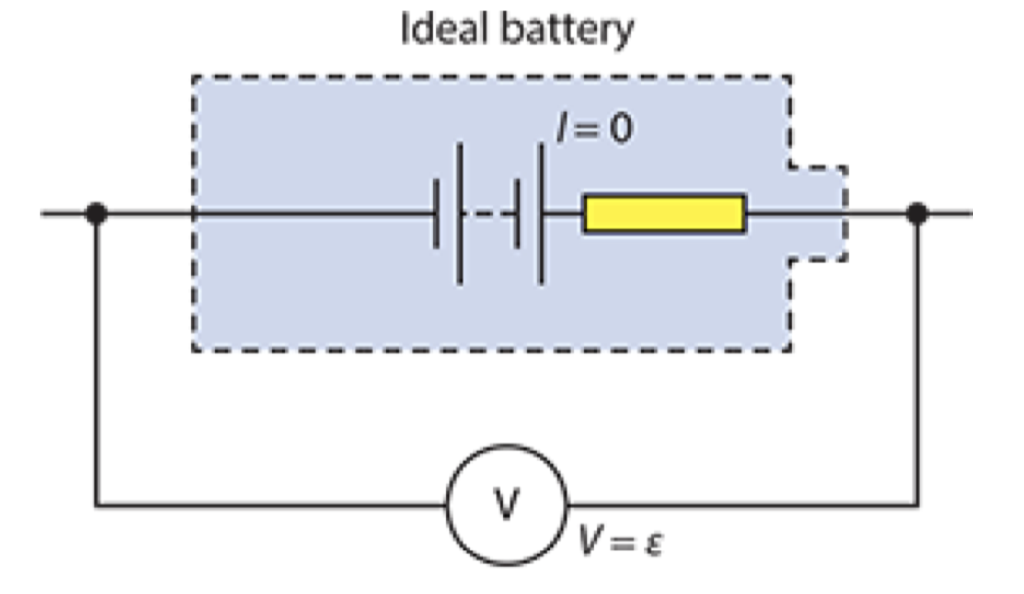
\includegraphics[width=0.4\linewidth]{截圖 2026-06-04 11.18.29.png}
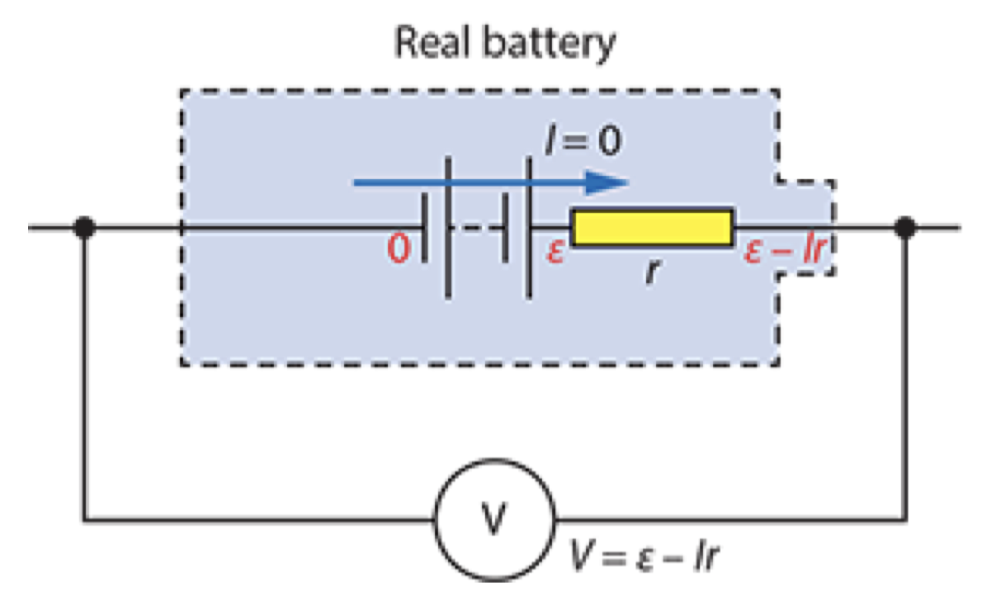
\includegraphics[width=0.4\linewidth]{截圖 2026-06-04 11.18.40.png}
\end{center}
We need to consider the existence of internal resistance in the real world: chemicals in cells (for example) also creates resistance in the cell.\\
The potential difference across the terminals of a battery is equal to the $e.m.f$ when there is no current in the circuit. It is less than the $e.m.f$ when there is current.\\
An $V-I$ graph can be used: $\varepsilon$ is the y-intercept, $r$ is the magnitude of the gradient of the line.
\begin{center}
\begin{tikzpicture}[>=Stealth, line width=0.7pt]

    % --- Color Definitions ---
    \definecolor{arrowblue}{RGB}{0, 112, 192}

    % =========================================================================
    % ========================== DIAGRAM A ====================================
    % =========================================================================
    \begin{scope}[xshift=0cm]

        % --- Coordinate Layout ---
        \coordinate (M) at (0, 2);
        \coordinate (N) at (6.5, 2);
        \coordinate (J1) at (1, 0.3);
        \coordinate (J2) at (4.5, 0.3);

        % 1. TOP PATH: BATTERY & OUTER LOOP
        \draw (M) -- (0,4) -- (2.8,4);
        
        % Crisp Textbook-Style Battery Symbol
        \draw[line width=0.8pt] (2.8, 4.35) -- (2.8, 3.65); % Positive plate
        \draw[line width=1.6pt] (3.1, 4.15) -- (3.1, 3.85); % Negative plate
        
        \draw (3.1,4) -- (6.5,4) -- (N);

        % 2. MIDDLE PATH: POTENTIOMETER / SLIDE WIRE
        % Slide Wire Bar (XY)
        \draw[fill=gray!60, draw=black, line width=0.6pt] (1, 1.88) rectangle (5.5, 2.12);
        
        % Labels for Slide Wire (Math mode for default Roman font)
        \node[above left, font=\small, yshift=-1pt] at (1, 2.12) {$X$};
        \node[above right, font=\small, yshift=-1pt] at (5.5, 2.12) {$Y$};

        % Main Circuit Connections to X and Y
        \draw (M) -- (1,2);
        \draw (5.5,2) -- (N);

        % Junction Dots M and N
        \fill (M) circle (2pt) node[left, xshift=-2pt] {$M$};
        \fill (N) circle (2pt) node[right, xshift=2pt] {$N$};

        % 3. LOWER BRANCH: METERS & PARALLEL CIRCUIT
        % Left Branch leading through Ammeter
        \draw (M) -- (0, 1.3);
        \draw[fill=white] (0, 0.9) circle (0.28) node {A};
        \draw (0, 0.5) -- (0, 0.3) -- (J1);

        % Parallel Node Dots
        \fill (J1) circle (1.8pt);
        \fill (J2) circle (1.8pt);

        % Top Parallel Path: Resistor R
        \draw (J1) to[R, l=$R$] (J2);

        % Bottom Parallel Path: Voltmeter V
        \draw (J1) -- (1, -0.5) -- (2.45, -0.5);
        \draw[fill=white] (2.75, -0.5) circle (0.28) node {V};
        \draw (3.05, -0.5) -- (4.5, -0.5) -- (J2);

        % Sliding Contact S
        \draw[->] (J2) -- (4.5, 1.88);
        \node[right, xshift=1pt, yshift=-2pt] at (4.5, 1.4) {$S$};

        % 4. CURRENT ARROWS (BLUE)
        % Top wire current (I)
        \draw[arrowblue, ->, line width=1.1pt] (2.1, 4.2) -- (1.5, 4.2);
        \node[above, xshift=-1pt] at (1.8, 4.2) {$I$};

        % Horizontal slider current (I1)
        \draw[arrowblue, ->, line width=1.1pt] (0.3, 1.7) -- (0.9, 1.7);
        \node[right, xshift=1pt] at (0.9, 1.6) {$I_1$};

        % Resistor branch current (I2)
        \draw[arrowblue, ->, line width=1.1pt] (1.2, 0.55) -- (1.7, 0.55);
        \node[right, xshift=1pt, yshift=1pt] at (1.6, 0.55) {$I_2$};

        % Right outer current (I)
        \draw[arrowblue, ->, line width=1.1pt] (5.7, 1.7) -- (6.3, 1.7);
        \node[right, xshift=1pt] at (6.3, 1.7) {$I$};
    \end{scope}

    % =========================================================================
    % ========================== DIAGRAM B ====================================
    % =========================================================================
    \begin{scope}[xshift=8.5cm]

        % --- Coordinate Layout ---
        \coordinate (M) at (0, 2);
        \coordinate (N) at (6.5, 2);
        \coordinate (J1) at (1, 0.3);
        \coordinate (J2) at (4.5, 0.3);
        \coordinate (S) at (4.5, 2);

        % 1. TOP PATH: BATTERY & OUTER LOOP
        \draw (M) -- (0,4) -- (2.8,4);
        
        % Crisp Textbook-Style Battery Symbol
        \draw[line width=0.8pt] (2.8, 4.35) -- (2.8, 3.65); % Positive plate
        \draw[line width=1.6pt] (3.1, 4.15) -- (3.1, 3.85); % Negative plate
        
        \draw (3.1,4) -- (6.5,4) -- (N);

        % 2. MIDDLE PATH: TWO SEPARATE RESISTORS (R1 & R2)
        \draw (M) to[R, l=$R_1$] (S) to[R, l=$R_2$] (N);

        % Junction Dots M, N, and S
        \fill (M) circle (2pt) node[left, xshift=-2pt] {$M$};
        \fill (N) circle (2pt) node[right, xshift=2pt] {$N$};
        \fill (S) circle (2pt) node[above, yshift=2pt] {$S$};

        % 3. LOWER BRANCH: METERS & PARALLEL CIRCUIT
        % Left Branch leading through Ammeter
        \draw (M) -- (0, 1.3);
        \draw[fill=white] (0, 0.9) circle (0.28) node {A};
        \draw (0, 0.5) -- (0, 0.3) -- (J1);

        % Parallel Node Dots
        \fill (J1) circle (1.8pt);
        \fill (J2) circle (1.8pt);

        % Top Parallel Path: Resistor R
        \draw (J1) to[R, l=$R$] (J2);

        % Bottom Parallel Path: Voltmeter V
        \draw (J1) -- (1, -0.5) -- (2.45, -0.5);
        \draw[fill=white] (2.75, -0.5) circle (0.28) node {V};
        \draw (3.05, -0.5) -- (4.5, -0.5) -- (J2);

        % Fixed vertical connection to equivalent junction point S
        \draw (J2) -- (S);

        % 4. CURRENT ARROWS (BLUE)
        % Top wire current (I)
        \draw[arrowblue, ->, line width=1.1pt] (2.1, 4.2) -- (1.5, 4.2);
        \node[above, xshift=-1pt] at (1.8, 4.2) {$I$};

        % Horizontal resistor R1 current (I1)
        \draw[arrowblue, ->, line width=1.1pt] (0.3, 1.7) -- (0.9, 1.7);
        \node[right, xshift=1pt] at (0.9, 1.7) {$I_1$};

        % Resistor branch current (I2)
        \draw[arrowblue, ->, line width=1.1pt] (1.2, 0.55) -- (1.7, 0.55);
        \node[right, xshift=1pt, yshift=1pt] at (1.6, 0.55) {$I_2$};

        % Right outer current (I)
        \draw[arrowblue, ->, line width=1.1pt] (5.2, 1.5) -- (5.8, 1.5);
        \node[right, xshift=1pt] at (5.8, 1.5) {$I$};
    \end{scope}

\end{tikzpicture}
\end{center}
By varying where the slider S connects to XY, different potential differences and currents are obtained for the device R.\\
The potential difference across $R$ now ranges from 0 to $\varepsilon$.
\newpage
% ===================== Unit C =====================
\unnumberedsection{Unit C Wave behaviour}
\section{Simple harmonic motion}
\subsection{Simple harmonic oscillations}
\begin{center}
  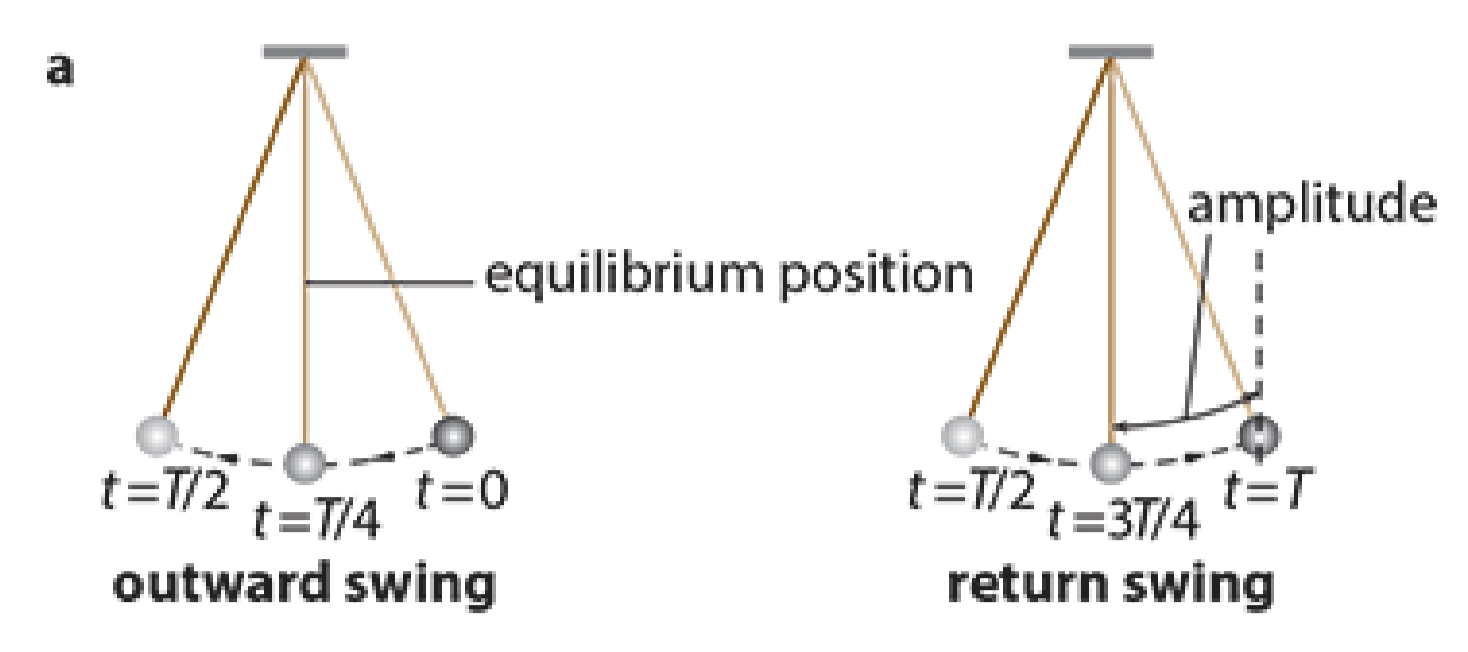
\includegraphics[width=0.6\linewidth]{截圖 2026-06-04 19.56.32.png}
\end{center}
Oscillations refer to back and forth motion that repeats. The body moves back and forth around an equilibrium position.
\begin{itemize}
  \item Period, $T=2\pi\sqrt{\dfrac{L}{g}}$ ($L$ is the length of the string), time taken to complete one full oscillation
  \item Amplitude, $A$, which is the maximum displacement away from the equilibrium position. 
  \item Frequency, $f=\dfrac{1}{T}$, number of oscillations in 1s.
  \item Acceleration (and the restoring force) is proportional to the opposite of displacement. $a=-\omega^2x$ ($x$ is the displacement)
  \item Angular frequency $\omega=\dfrac{2\pi}{T}=2\pi f$ 
\end{itemize}
\begin{center}
  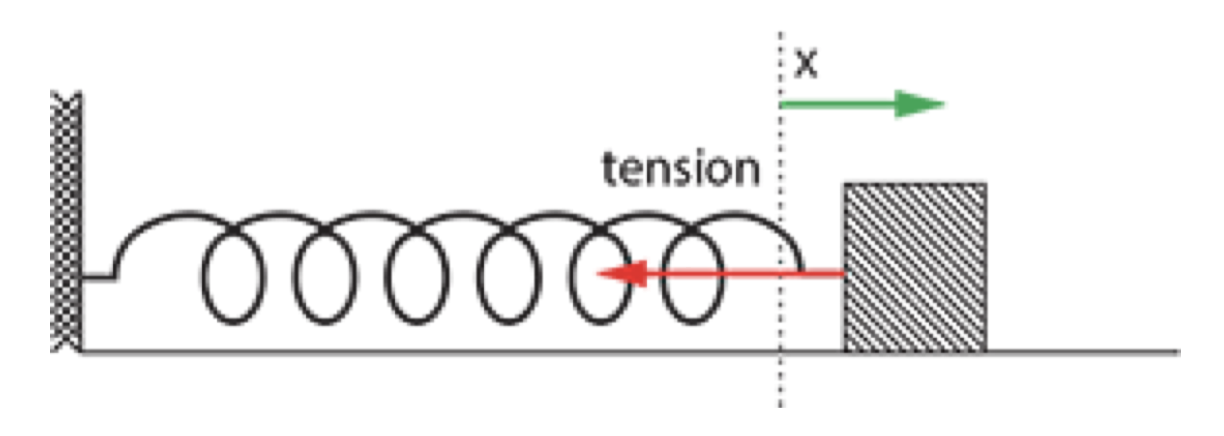
\includegraphics[width=0.35\linewidth]{截圖 2026-06-04 20.03.37.png}
  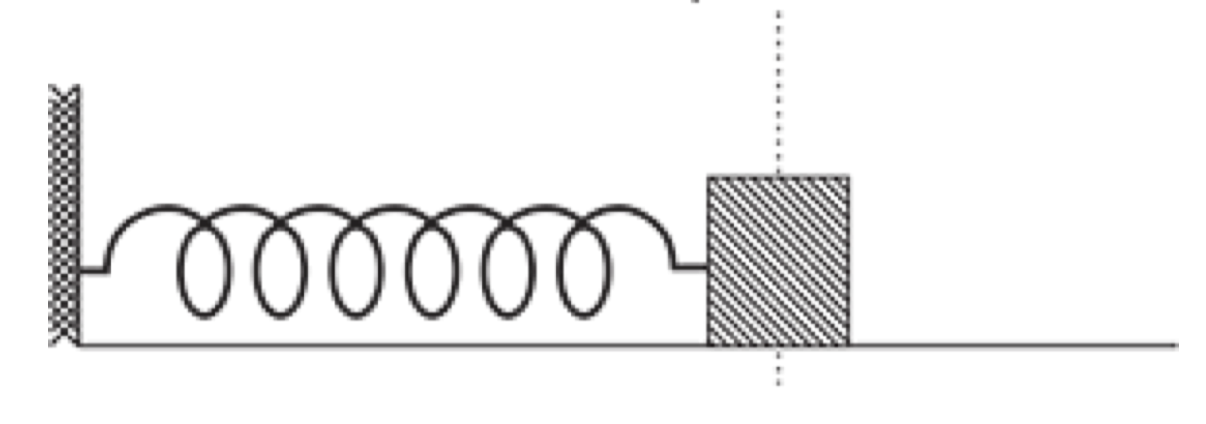
\includegraphics[width=0.35\linewidth]{截圖 2026-06-04 20.04.03.png}
\end{center}
In this case:
\begin{itemize}
  \item $\displaystyle a=-\dfrac{k}{m}x$
  \item $\omega=\sqrt{\dfrac{k}{m}}$
  \item $T=2\pi\sqrt{\dfrac{m}{k}}$
\end{itemize}
In SHM:
\begin{itemize}
  \item the period does not depend on amplitude
  \item the amplitude stays constant as time goes on.
\end{itemize}
A graph of acceleration against displacement gives a straight line through origin with a slope of $-\omega^2$.\\
Phase difference between two oscillations: $\Delta \phi=\dfrac{\Delta t}{T}\times 2\pi\ \text{rad}$, where $\Delta t$ is the separation in time between two neighbouring peaks. (2+ same SHMs have different peaks, started with different displacements)
\subsection{Details of simple harmonic motion}
Displacement $x$ as a function of time is expressed as
\[x=x_0\sin(\omega t+\phi)\]
where $x_0$ is the amplitude and $\phi$ is the phase angle.
\[v=\omega x_0\cos(\omega t+\phi);\ v_\text{max}=\omega x_0\]
\[a=-\omega^2x_0\sin(\omega t+\phi);\ a_\text{max}=\omega^2x_0\]
Phase difference can be expressed as magnitude of differences between two phase angles.
\[\Delta \phi=|\phi_1-\phi_2|\]
\subsection{Energy in simple harmonic motion}
$E_T=E_P+E_K=$ constant (in the absence of other resistance forces, energy is conserved)
\begin{center}
  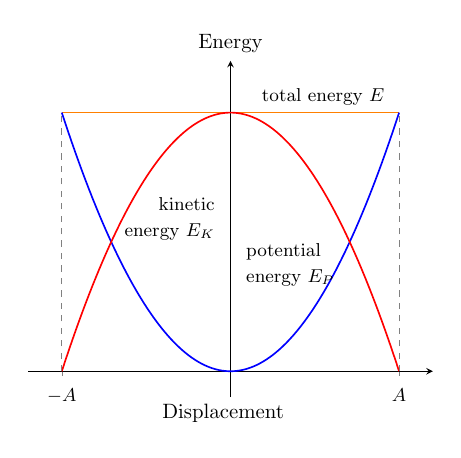
\begin{tikzpicture}[scale=0.75]
    \begin{axis}[
        % Axis configuration
        axis lines=middle,
        xmin=-1.2, xmax=1.2,
        ymin=-0.1, ymax=1.2,
        xlabel=Displacement,
        ylabel=Energy,
        x label style={at={(axis description cs:0.65,0)},anchor=north east},
        y label style={at={(axis description cs:0.5,1.1)},anchor=north},
        xtick={-1, 0, 1},
        xticklabels={$-A$, $0$, $A$},
        ytick=\empty, % Hide y-axis ticks
        % Tick formatting
        x tick label style={below=1mm, font=\small},
    ]
        % Total Energy (orange horizontal line)
        \draw[orange, thick] (-1, 1) -- (1, 1);
        
        % Potential Energy (blue parabola: E_P = E * (x/A)^2, here E=1, A=1)
        \addplot[domain=-1:1, blue, thick, samples=100] {x^2};
        
        % Kinetic Energy (red inverted parabola: E_K = E - E_P = E * (1 - (x/A)^2), here E=1, A=1)
        \addplot[domain=-1:1, red, thick, samples=100] {1 - x^2};
        
        % Dashed lines at limits -A and A
        \draw[dashed, gray] (-1, 0) -- (-1, 1);
        \draw[dashed, gray] (1, 0) -- (1, 1);
        
        % Text labels
        \node[anchor=south] at (axis cs:0.55, 1.0) {\small total energy $E$};
        \node[anchor=north east] at (axis cs:-0.05, 0.7) {\small kinetic};
        \node[anchor=north east] at (axis cs:-0.05, 0.6) {\small energy $E_K$};
        \node[anchor=south west] at (axis cs:0.05, 0.4) {\small potential};
        \node[anchor=south west] at (axis cs:0.05, 0.3) {\small energy $E_P$};
        
    \end{axis}
\end{tikzpicture}
\end{center}
You will need to deduce how kinetic and potential energy varies with time from a given displacement-time graph:
\begin{center}
  \begin{tikzpicture}[scale=0.7]

% --- Graph 1: Displacement vs Time ---
\begin{axis}[
    name=axis1,
    anchor=south west,
    at={(0,0)},
    width=14cm,
    height=7cm,
    % Axis range and origin
    xmin=0, xmax=5,
    ymin=-5.2, ymax=5.2,
    axis lines=middle,
    % Axis labels with positioning
    xlabel={$t$/s},
    xlabel style={at={(axis cs: 5,0)}, anchor=west, xshift=1.5ex},
    ylabel={$x$/cm},
    ylabel style={at={(axis description cs:0,1)},anchor=south}, % Shift up and left slightly
    % Grid and tick configuration
    grid=both,
    grid style={line width=.1pt, draw=gray!20},
    minor tick num=4, % 4 minor ticks between major, giving 5 subdivisions
    minor grid style={line width=.05pt, draw=gray!10},
    major tick style={line width=0.5pt, draw=black},
    % Specify major tick positions
    xtick={1, 2, 3, 4, 5},
    ytick={-4, -2, 0, 2, 4},
    % Define specific tick labels if needed, or rely on auto
    % xticklabels={1, 2, 3, 4, 5},
    yticklabels={-4, -2, 0, 2, 4},
    % Axis arrow head
    axis line style={-Stealth, black, thin},
    ticklabel style={fill=white, inner sep=1.5pt}, % Ensure labels are clear
]
    % Plot the red curve: x(t) = 4 * cos(pi/2 * t)
    \addplot[
        domain=0:5,
        samples=100,
        red,
        line width=1.0pt,
    ] {4*cos(90*x)}; % cos uses degrees in pgfplots unless specified

    % Special label at the origin for t=0 and x=0
    \node[anchor=north east, yshift=-1ex, xshift=-1ex] at (axis cs:0,0) {\textbf{0}};
\end{axis}
\end{tikzpicture}\\
\begin{tikzpicture}[scale=0.7]
% --- Graph 2: Energy vs Time ---
\begin{axis}[
    clip=false,
    name=axis2,
    anchor=south west,
    at={(axis1.below south west)}, % Position below the first graph
    yshift=-1.0cm,
    width=14cm,
    height=7cm,
    % Axis range and origin
    xmin=0, xmax=5,
    ymin=-2, ymax=45,
    axis lines=middle,
    % Axis labels with positioning
    xlabel={$t$/s},
    ylabel={$E$/mJ},
    ylabel style={at={(axis description cs:0,1)},anchor=south}, % Shift up and left slightly
    xlabel style={at={(axis cs: 5,0)}, anchor=west, xshift=1.5ex},
    % Grid and tick configuration
    grid=both,
    grid style={line width=.1pt, draw=gray!20},
    minor tick num=4, % 4 minor ticks between major, giving 5 subdivisions
    minor grid style={line width=.05pt, draw=gray!10},
    major tick style={line width=0.5pt, draw=black},
    % Specify major tick positions
    xtick={1, 2, 3, 4, 5},
    ytick={0, 10, 20, 30, 40},
    % Define specific tick labels
    xticklabels={1, 2, 3, 4, 5},
    yticklabels={0, 10, 20, 30, 40},
    % Axis arrow head
    axis line style={-Stealth, black, thin},
    ticklabel style={fill=white, inner sep=1.5pt}, % Ensure labels are clear
]
    % Plot the red curve (Kinetic Energy): E_k(t) = 40 * sin^2(pi/2 * t)
    \addplot[
        domain=0:5,
        samples=150,
        red,
        line width=1.0pt,
    ] {40*(sin(90*x)^2)};

    % Plot the blue curve (Potential Energy): E_p(t) = 40 * cos^2(pi/2 * t)
    \addplot[
        domain=0:5,
        samples=150,
        blue,
        line width=1.0pt,
    ] {40*(cos(90*x)^2)};

    % Annotations
    \draw[thin] (axis cs: 4.8, 33) -- (axis cs: 5.1, 33) node[right, red, fill=white, inner sep=2pt] {kinetic energy};
    \draw[thin] (axis cs: 4.8, 8) -- (axis cs: 5.1, 8) node[right, blue, fill=white, inner sep=2pt] {potential energy};

    % Special label at the origin for t=0
    \node[anchor=north east, yshift=-1ex, xshift=-1ex] at (axis cs:0,0) {\textbf{0}};
\end{axis}

\end{tikzpicture}
\end{center}
\subsection{More about energy in SHM}
\[E_K=\dfrac{1}{2}m\omega^2(x_0^2-x^2)\]
\[E_P=\dfrac{1}{2}m\omega^2x^2\]
\[E_T=\dfrac{1}{2}m\omega^2x_0^2\]
\[v=\pm \omega\sqrt{x_0^2-x^2}\]
\section{The wave model}
\subsection{Mechanical pulses and waves}
A mechanical wave is a disturbance that travels in a medium through oscillations of the particles of the medium. A wave transfers energy and momentum. The direction of propagation of the wave is the direction of energy transfer.
\begin{itemize}
  \item Wavelength, $\lambda$, length of one full wave / distance from crest to crest or trough to trough
  \item Period, $T$, time to create one full wave
  \item Frequency, $f=\dfrac{1}{T}$, the number of full waves created in 1s
  \item Speed, $v=\dfrac{\lambda}{T}=f\lambda$
\end{itemize}
\subsection{Transverse and longitudinal waves}
Transverse: the displacement of the particles of the medium is at right angles to the direction of energy transfer.\\
As a wave propagates through a medium, the particles of the medium perform SHM with a frequency that is the same as that of the wave.
\begin{center}
  \begin{tikzpicture}[>=Stealth]

    % --- Color Palettes matching the image ---
    \definecolor{wavebrown}{RGB}{180, 130, 85}
    \definecolor{arrowgreen}{RGB}{75, 165, 100}
    \definecolor{arrowred}{RGB}{220, 50, 45}

    % --- Wave Parameters ---
    % y = Amplitude * sin(90 * x) -> Period = 4 units
    \def\amplitude{1.2}
    
    % --- 1. Draw the Green Oscillation Arrows ---
    % All arrows share the exact same vertical span (from -Amplitude to +Amplitude)
    
    % Arrow 1 (on the downward slope)
    \coordinate (A1) at (1.65, 0);
    \draw[<->, line width=1.5pt, arrowgreen] ($(A1)-(0,\amplitude)$) -- ($(A1)+(0,\amplitude)$);
    
    % Arrow 2 (exactly at the trough)
    \coordinate (A2) at (3.0, 0);
    \draw[<->, line width=1.5pt, arrowgreen] ($(A2)-(0,\amplitude)$) -- ($(A2)+(0,\amplitude)$);
    
    % Arrow 3 (on the next downward slope, exactly 1 period away)
    \coordinate (A3) at (5.65, 0);
    \draw[<->, line width=1.5pt, arrowgreen] ($(A3)-(0,\amplitude)$) -- ($(A3)+(0,\amplitude)$);

    % --- 2. Draw the Continuous Wave Curve ---
    \draw[line width=3.5pt, wavebrown, line cap=round] 
        plot[domain=-0.3:7.6, samples=200] (\x, {\amplitude*sin(\x*90)});

    % --- 3. Draw the Particles (sitting perfectly on the wave) ---
    \fill[wavebrown] (1.65, {\amplitude*sin(1.65*90)}) circle (0.18);
    \fill[wavebrown] (3.0,  {\amplitude*sin(3.0*90)})  circle (0.18);
    \fill[wavebrown] (5.65, {\amplitude*sin(5.65*90)}) circle (0.18);

    % --- 4. Draw the Red Wave Propagation Arrow ---
    \draw[->, line width=2pt, arrowred, >=Stealth] (1.8, 1.8) -- (4.2, 1.8);

\end{tikzpicture}
\end{center}
\begin{center}
  \begin{tikzpicture}[>=Stealth,scale=1.2]

    % --- Color definitions matching the image ---
    \definecolor{nowblue}{RGB}{35, 45, 140}       % Darker blue for "now"
    \definecolor{laterblue}{RGB}{45, 125, 205}   % Brighter/lighter blue for "a bit later"

    % --- Wave Parameters ---
    \def\amplitude{1.1}
    % Solid wave: y = sin(x * 90)
    % Dashed wave is shifted to the right by 0.7 units: y = sin((x - 0.7) * 90)

    % --- 1. Vertical Dashed Reference Lines ---
    % Line 1: Passing through the crest of the dashed wave (x = 1.7)
    \draw[dashed, gray!80, thick] (1.7, -1.4) -- (1.7, 1.4);
    
    % Line 2: Passing through the trough of the solid wave (x = 3.0)
    \draw[dashed, gray!80, thick] (3.0, -1.4) -- (3.0, 1.1);
    
    % Line 3: Passing through the trough of the dashed wave (x = 3.7)
    \draw[dashed, gray!80, thick] (3.7, -1.4) -- (3.7, 1.1);
    
    % Line 4: One full wavelength past Line 1 (x = 5.7)
    \draw[dashed, gray!80, thick] (5.7, -1.4) -- (5.7, 1.4);


    % --- 2. Wave Curves ---
    % "now" wave (Solid Dark Blue)
    \draw[line width=1.5pt, nowblue] 
        plot[domain=-0.2:6.2, samples=200] (\x, {\amplitude*sin(\x*90)});

    % "a bit later" wave (Dashed Lighter Blue)
    \draw[line width=1.5pt, laterblue, dashed] 
        plot[domain=-0.2:6.2, samples=200] (\x, {\amplitude*sin((\x-0.7)*90)});


% --- 3. Particles / Dots ---
    % Dots on Line 1
    \filldraw[fill=nowblue, draw=black!80, ultra thin] (1.7, {\amplitude*sin(1.7*90)}) circle (0.14);
    \filldraw[fill=laterblue, draw=black!80, ultra thin] (1.7, {\amplitude*sin((1.7-0.7)*90)}) circle (0.14);

    % Dots on Line 2
    \filldraw[fill=nowblue, draw=black!80, ultra thin] (3.0, {\amplitude*sin(3.0*90)}) circle (0.14);
    \filldraw[fill=laterblue, draw=black!80, ultra thin] (3.0, {\amplitude*sin((3.0-0.7)*90)}) circle (0.14);

    % Dots on Line 3
    \filldraw[fill=nowblue, draw=black!80, ultra thin] (3.7, {\amplitude*sin(3.7*90)}) circle (0.14);
    \filldraw[fill=laterblue, draw=black!80, ultra thin] (3.7, {\amplitude*sin((3.7-0.7)*90)}) circle (0.14);

    % Dots on Line 4
    \filldraw[fill=nowblue, draw=black!80, ultra thin] (5.7, {\amplitude*sin(5.7*90)}) circle (0.14);
    \filldraw[fill=laterblue, draw=black!80, ultra thin] (5.7, {\amplitude*sin((5.7-0.7)*90)}) circle (0.14);

    % --- 4. Motion & Label Arrows ---
    % Top wave propagation arrow
    \draw[->, line width=1.2pt, black!90] (0.9, 1.5) -- (1.7, 1.5);

    % "now" label and arrow
    \coordinate (nowTarget) at (0.35, {\amplitude*sin(0.35*90)});
    \draw[<-, >=Stealth, shorten <=2pt, black!80] (nowTarget) -- (0.35, -1.3) node[below, black] {now};

    % "a bit later" label and arrow
    \coordinate (laterTarget) at (1.3, {\amplitude*sin((1.3-0.7)*90)});
    \draw[<-, >=Stealth, shorten <=2pt, black!80] (laterTarget) -- (1.5, -1.8) node[below, black] {a bit later};

\end{tikzpicture}
\end{center}
\begin{center}
  \begin{tikzpicture}[>=Stealth]

    % --- Color Palette ---
    \definecolor{gridblue}{RGB}{215, 228, 242}
    \definecolor{wavered}{RGB}{226, 62, 53}
    \definecolor{darkgray}{RGB}{80, 80, 80}

    % ==========================================
    % LEFT GRAPH: Displacement vs Distance
    % ==========================================
    \begin{scope}[x=3.5cm, y=0.45cm]
        
        % 1. Fine Grid Background
        \foreach \x in {0, 0.05, ..., 2.1} {
            \draw[line width=0.4pt, gridblue] (\x, -4.5) -- (\x, 4.5);
        }
        \foreach \y in {-4.5, -4.0, ..., 4.5} {
            \draw[line width=0.4pt, gridblue] (0, \y) -- (2.1, \y);
        }
        
        % 2. Axes
        \draw[line width=0.8pt, ->] (0, 0) -- (2.15, 0) node[below, yshift=-0.4cm, xshift=0.3cm] {Distance/m};
        \draw[line width=0.8pt, ->] (0, -4.5) -- (0, 4.8) node[left, yshift=0.5cm, xshift=1.5cm] {Displacement/cm};
        
        % 3. Axis Ticks & Labels
        \foreach \x in {0.5, 1.0, 1.5, 2.0} {
            \draw[line width=0.8pt] (\x, 0) -- (\x, -0.15) node[below, font=\small] {\x};
        }
        \foreach \y in {-4, -2, 2, 4} {
            \draw[line width=0.8pt] (0, \y) -- (-0.03, \y) node[left, font=\small] {\y};
        }
        \node[left, font=\small, xshift=-0.05cm, yshift=-0.2cm] at (0,0) {0};
        
        % 4. Wave Curve (y = 4 * cos(5 * pi * x))
        \draw[line width=1.5pt, wavered, line cap=round] 
            plot[domain=0:2.1, samples=250] (\x, {4*cos(\x*5*180)});
            
        % 5. Annotations ($\lambda$ and Amplitude)
        \draw[<->, line width=0.7pt, darkgray] (0, 4.15) -- (0.4, 4.15);
        \node[above, font=\small, darkgray, yshift=-0.05cm] at (0.2, 4.15) {$\lambda$};
        
        \draw[<->, line width=0.7pt, darkgray] (1.2, 0) -- (1.2, 4.0);
        \node[above, font=\small, darkgray] at (1.2, 4.1) {amplitude $A$};

    \end{scope}

    % ==========================================
    % RIGHT GRAPH: Displacement vs Time
    % ==========================================
    \begin{scope}[x=0.65cm, y=0.45cm, xshift=9.5cm]
        
        % 1. Fine Grid Background
        \foreach \x in {0, 0.5, ..., 10.5} {
            \draw[line width=0.4pt, gridblue] (\x, -4.5) -- (\x, 4.5);
        }
        \foreach \y in {-4.5, -4.0, ..., 4.5} {
            \draw[line width=0.4pt, gridblue] (0, \y) -- (10.5, \y);
        }
        
        % 2. Axes
        \draw[line width=0.8pt, ->] (0, 0) -- (10.8, 0) node[below, yshift=-0.4cm, xshift=0.3cm] {$t$/ms};
        \draw[line width=0.8pt, ->] (0, -4.5) -- (0, 4.8) node[left, yshift=0.4cm, xshift=1.5cm] {Displacement/cm};
        
        % 3. Axis Ticks & Labels
        \foreach \x in {2, 4, 6, 8, 10} {
            \draw[line width=0.8pt] (\x, 0) -- (\x, -0.15) node[below, font=\small] {\x};
        }
        \foreach \y in {-4, -2, 2, 4} {
            \draw[line width=0.8pt] (0, \y) -- (-0.15, \y) node[left, font=\small] {\y};
        }
        \node[left, font=\small, xshift=-0.05cm, yshift=-0.2cm] at (0,0) {0};
        
        % 4. Wave Curve (y = -4 * sin(0.5 * pi * t))
        \draw[line width=1.5pt, wavered, line cap=round] 
            plot[domain=0:10.5, samples=250] (\x, {-4*sin(\x*0.5*180)});
            
        % 5. Annotations (Period T)
        \draw[<->, line width=0.7pt, darkgray] (3.0, 4.15) -- (7.0, 4.15);
        \node[above, font=\small, darkgray, yshift=-0.05cm] at (5.0, 4.15) {period $T$};

    \end{scope}
\end{tikzpicture}\\
Displacement-distance and Displacement-time (displacement of one specific point)
\end{center}
Longitudinal waves: the displacement is parallel to the direction of energy transfer.
\begin{center}
  \begin{tikzpicture}[>=Stealth, ]

    % --- Color Palette ---
    \definecolor{wavered}{RGB}{221, 44, 0}
    \definecolor{springgray}{RGB}{40, 40, 40}

    % --- 1. Longitudinal Slinky Wave ---
    % Using a smooth parametric equation where wave density modulation variations 
    % naturally crowd or spread the continuous helical loops.
    % 
    % Compression centers occur at x = 2.5 and x = 7.5
    % Rarefaction center occurs at x = 5.0
    \draw[line width=1.0pt, springgray, line cap=round] 
        plot[domain=0.5:10.5, samples=1000] 
        ({ \x + 0.62*sin(\x*(360/5.0)) + 0.08*sin(\x*1440) }, { 0.45*cos(\x*1440) });

    % --- 2. Source Vibration Indicator (Left End) ---
    \draw[<->, line width=1.2pt, wavered] (-0.8, 0) -- (-0.1, 0);

    % --- 3. Annotations & Labels ---
    
    % Compression Arrow & Label
    \draw[->, line width=1.0pt, wavered] (2.5, 1.3) -- (2.5, 0.6);
    \node[above, font=\small, text=springgray] at (2.5, 1.3) {compression};

    % Rarefaction Arrow & Label
    \draw[->, line width=1.0pt, wavered] (5.0, 1.3) -- (5.0, 0.6);
    \node[above, font=\small, text=springgray] at (5.0, 1.3) {rarefaction};

    % Wavelength Measurement Line & Label
    \draw[<->, line width=1.0pt, wavered] (2.5, -0.9) -- (7.5, -0.9);
    \node[below, font=\small, text=springgray, yshift=-0.05cm] at (5.0, -0.9) {wavelength};

\end{tikzpicture}
\end{center}
Compression: a region of higher than normal density\\
Rarefaction: a region of lower than normal density\\
\textbf{You cannot tell whether a wave is transverse or longitudinal by looking at displacement-distance or displacement-time graphs. The graphs look the same for both.}
\begin{center}
  \begin{tikzpicture}[>=Stealth, ]

    % --- Color Palette ---
    \definecolor{gridblue}{RGB}{215, 228, 242}
    \definecolor{waveblue}{RGB}{30, 110, 190}
    \definecolor{arrowred}{RGB}{226, 62, 53}
    
    \definecolor{dotblue}{RGB}{50, 110, 190}
    \definecolor{dotred}{RGB}{226, 62, 53}
    \definecolor{dotgreen}{RGB}{60, 160, 80}

    % ==========================================
    % 1. DISPLACEMENT GRAPH
    % ==========================================
    \begin{scope}[x=1.6cm, y=0.45cm]
        
        % Fine Grid Background
        \foreach \x in {0, 0.2, ..., 5.0} {
            \draw[line width=0.4pt, gridblue] (\x, -5) -- (\x, 5);
        }
        \foreach \y in {-5, -4.8, ..., 5.0} {
            \draw[line width=0.4pt, gridblue] (0, \y) -- (5, \y);
        }
        
        % Main Axes
        \draw[line width=1.0pt, black] (0, -5) -- (0, 5);
        \draw[line width=1.0pt, black] (0, 0) -- (5, 0);
        
        % Y-Axis Ticks & Labels
        \foreach \y in {-5, -4, -3, -2, -1, 1, 2, 3, 4, 5} {
            \draw[line width=0.8pt] (0, \y) -- (-0.08, \y);
            \node[left, font=\small] at (-0.1, \y) {\y};
        }
        \node[left, font=\small, xshift=-0.1cm, yshift=-0.15cm] at (0,0) {0};
        
        % X-Axis Ticks & Labels
        \foreach \x in {1, 2, 3, 4, 5} {
            \draw[line width=0.8pt] (\x, 0) -- (\x, -0.15);
            \node[below, font=\small, yshift=-0.05cm] at (\x, 0) {\x};
        }
        
        % Axis Labels
        \node[rotate=90, font=\small] at (-0.5, 0) {Displacement $y$/mm};
        \node[font=\small] at (2.5, -6) {Distance $x$/cm};
        
        % Sine Wave Curve
        \draw[line width=1.6pt, waveblue, line cap=round] 
            plot[domain=0:5, samples=200] (\x, {5*sin(\x*90)});
            
        % Red Dashed Particle Displacement Direction Arrows
        \draw[->, arrowred, line width=1.2pt, dashed] (0.15, 0.6) -- (0.55, 0.6);
        \draw[->, arrowred, line width=1.2pt, dashed] (0.85, 0.6) -- (1.25, 0.6);
        \draw[->, arrowred, line width=1.2pt, dashed] (1.45, 0.6) -- (1.85, 0.6);
        
        \draw[<-, arrowred, line width=1.2pt, dashed] (2.15, 0.6) -- (2.55, 0.6);
        \draw[<-, arrowred, line width=1.2pt, dashed] (2.85, 0.6) -- (3.25, 0.6);
        \draw[<-, arrowred, line width=1.2pt, dashed] (3.45, 0.6) -- (3.85, 0.6);
        
        \draw[->, arrowred, line width=1.2pt, dashed] (4.15, 0.6) -- (4.55, 0.6);
        \draw[->, arrowred, line width=1.2pt, dashed] (4.70, 0.6) -- (5.00, 0.6);

    \end{scope}

    % ==========================================
    % 2. PARTICLE POSITION VISUALIZATION
    % ==========================================
    \begin{scope}[x=1.6cm, y=0.45cm]
        
        % Plot text labels and row 1 dots safely using an integer counter
        \foreach \i / \labeltext in {0/0, 1/0.5, 2/1, 3/1.5, 4/2, 5/2.5, 6/3, 7/3.5, 8/4, 9/4.5} {
            \pgfmathsetmacro{\x}{\i * 0.5}
            
            % Labels
            \node[font=\small, anchor=south] at (\x, -7.8) {\labeltext};
            
            % Row 1: Equilibrium Dots
            \ifnum\i=4
                \fill[dotred] (\x, -8.5) circle (2.5pt);
            \else
                \ifnum\i=8
                    \fill[dotgreen] (\x, -8.5) circle (2.5pt);
                \else
                    \fill[dotblue] (\x, -8.5) circle (2.5pt);
                \fi
            \fi
        }
        
        % Tailoring the final "5 cm" boundary point configuration
        \node[font=\small, anchor=south west] at (5.0, -7.8) {5 cm};
        \fill[dotblue] (5.0, -8.5) circle (2.5pt);

        % Row 2: Actual Displaced Positions plotted directly on the fly
        \foreach \i in {0, 1, ..., 10} {
            \pgfmathsetmacro{\x}{\i * 0.5}
            \pgfmathsetmacro{\newx}{\x + 0.25*sin(\x*90)}
            
            \ifnum\i=4
                \fill[dotred] (\newx, -9.8) circle (2.5pt);
            \else
                \ifnum\i=8
                    \fill[dotgreen] (\newx, -9.8) circle (2.5pt);
                \else
                    \fill[dotblue] (\newx, -9.8) circle (2.5pt);
                \fi
            \fi
        }

    \end{scope}

\end{tikzpicture}\\
Positive displacement means moving right, negative displacement means moving left.
\end{center}
Phase difference is defined as
\[\Delta \phi =2\pi \dfrac{\Delta x}{\lambda}\]
where $\Delta x$ is the difference between consecutive peaks. The same formula can also be used to find the phase difference between two different points on the same wave.
\subsection{Electromagnetic waves}
\begin{center}
\begin{tikzpicture}[
    x={(0.9cm,-0.12cm)}, 
    y={(0cm,1.0cm)}, 
    z={(-0.45cm,-0.35cm)}, 
    >=Stealth, 
]

    % --- Color Palette ---
    \definecolor{efield}{RGB}{236, 0, 140}   % Vibrant Magenta
    \definecolor{mfield}{RGB}{0, 160, 230}   % Clean Cyan
    \definecolor{velred}{RGB}{230, 30, 30}   % Propagation Arrow Red

    % ==========================================
    % 1. AXES SYSTEM
    % ==========================================
    \draw[->, line width=0.8pt] (0,0,0) -- (9.0,0,0) node[right, xshift=2pt] {$x$};
    \draw[->, line width=0.8pt] (0,0,0) -- (0,2.5,0) node[above] {$y$};
    \draw[->, line width=0.8pt] (0,0,0) -- (0,0,3.2) node[below left] {$z$};

    % ==========================================
    % 2. FIELD VECTORS (ARROWS)
    % ==========================================
    % Plotted at regular intervals, skipping the nodes (0, 2, 4, 6, 8)
    \foreach \x in {0.4, 0.8, 1.2, 1.6, 2.4, 2.8, 3.2, 3.6, 4.4, 4.8, 5.2, 5.6, 6.4, 6.8, 7.2, 7.6} {
        % Electric Field Vectors (vertical along y-axis)
        \draw[->, efield, line width=0.7pt] (\x, 0, 0) -- (\x, {1.4*sin(\x*90)}, 0);
        
        % Magnetic Field Vectors (horizontal along z-axis)
        \draw[->, mfield, line width=0.7pt] (\x, 0, 0) -- (\x, 0, {1.4*sin(\x*90)});
    }

    % ==========================================
    % 3. WAVE SINE CURVES
    % ==========================================
    % Electric Field Curve (xy-plane)
    \draw[line width=1.5pt, efield, domain=0:8, samples=150, line cap=round] 
        plot (\x, {1.4*sin(\x*90)}, 0);

    % Magnetic Field Curve (xz-plane)
    \draw[line width=1.5pt, mfield, domain=0:8, samples=150, line cap=round] 
        plot (\x, 0, {1.4*sin(\x*90)});

    % ==========================================
    % 4. LABELS & ANNOTATIONS
    % ==========================================
    
    % Wavelength (λ) indicator spanning from first crest to second crest of E-field
    \draw[dashed, gray, line width=0.5pt] (1.0, 1.4, 0) -- (1.0, 2.4, 0);
    \draw[dashed, gray, line width=0.5pt] (5.0, 1.4, 0) -- (5.0, 2.4, 0);
    \draw[<->, line width=0.6pt] (1.0, 2.3, 0) -- (5.0, 2.3, 0) 
        node[midway, above, fill=white, inner sep=2pt] {wavelength $\lambda$};

    % Propagation velocity vector (c)
    \draw[->, velred, line width=1.2pt] (5.2, 1.7, 0) -- (6.2, 1.7, 0) 
        node[right, black, font=\small\bfseries] {$c\approx 3.0\times 10^8\ \text{m/s}$};

    % Electric Field text label with pointer line
    \draw[black, line width=0.5pt] (7.2, -1.1, 0) -- (8.2, -1.8, 0) 
        node[right, yshift=-2pt] {electric field};

    % Magnetic Field text label with pointer line
    \draw[black, line width=0.5pt] (1.0, 0, 1.0) -- (0.8, -0.8, 2.2) 
        node[below left, xshift=0.3cm] {magnetic field};

\end{tikzpicture}\\
An oscillating electric field produces an oscillating magnetic field such that the two are at right angles to each other and both propagate in space at the speed of light. Two fields are in phase.
\\
\begin{tikzpicture}[>=Stealth, font=\scriptsize]

    % --- Custom Spectrum Shading Definition ---
    \pgfdeclarehorizontalshading{spectrum}{2cm}{
        color(0.00cm)=(red);
        color(0.15cm)=(orange);
        color(0.30cm)=(yellow);
        color(0.50cm)=(green);
        color(0.65cm)=(cyan);
        color(0.80cm)=(blue);
        color(1.00cm)=(violet)
    }

    % ==========================================
    % 1. TOP AXIS: INCREASING FREQUENCY
    % ==========================================
    \node[anchor=west] at (-0.5, 2.1) {increasing frequency (Hz)};
    \draw[->, line width=0.6pt] (3.1, 2.1) -- (4.2, 2.1);

    % ==========================================
    % 2. MAIN ELECTROMAGNETIC SPECTRUM BAR
    % ==========================================
    \draw[line width=0.6pt] (-0.5, 0) rectangle (12.5, 0.9);
    \shade[shading=spectrum] (5.7, 0) rectangle (6.3, 0.9);

    % Section Labels inside the bar (inherits \scriptsize)
    \node at (0.25, 0.45) {AM radio};
    \node at (1.6, 0.45) {FM radio};
    \node at (3.2, 0.45) {microwaves};
    \node at (4.6, 0.45) {infrared};
    \node at (7.4, 0.45) {ultraviolet};
    \node at (9.1, 0.45) {X-rays};
    \node at (11.3, 0.45) {gamma rays};

    % Top Ticks & Numerical Labels (Frequency)
    \foreach \x / \freq in {
        0/{10^6}, 1.5/{10^8}, 3.0/{10^{10}}, 4.5/{10^{12}}, 
        6.0/{10^{14}}, 7.5/{10^{16}}, 9.0/{10^{18}}, 10.5/{10^{20}}, 12.0/{10^{22}}
    } {
        \draw[line width=0.5pt] (\x, 0.9) -- (\x, 1.02);
        \node[above, yshift=-3pt] at (\x, 1.02) {$\freq$};
    }

    % Bottom Ticks & Numerical Labels (Wavelength)
    \foreach \x / \wave in {
        0/{300}, 1.5/{3}, 3.0/{0.03}, 4.5/{3 \times 10^{-4}}, 
        6.0/{3 \times 10^{-6}}, 7.5/{3 \times 10^{-8}}, 9.0/{3 \times 10^{-10}}, 
        10.5/{3 \times 10^{-12}}, 12.0/{3 \times 10^{-14}}
    } {
        \draw[line width=0.5pt] (\x, 0) -- (\x, -0.12);
        \node[below, yshift=3pt] at (\x, -0.12) {$\wave$};
    }

    % ==========================================
    % 3. BOTTOM AXIS: INCREASING WAVELENGTH
    % ==========================================
    \node[anchor=west] at (0.8, -0.9) {increasing wavelength (m)};
    \draw[->, line width=0.6pt] (0.6, -0.9) -- (-0.5, -0.9);

    % ==========================================
    % 4. MAGNIFIED VISIBLE LIGHT CALLOUT
    % ==========================================
    \draw[line width=0.4pt, black] (5.7, 0) -- (4.0, -2.0);
    \draw[line width=0.4pt, black] (6.3, 0) -- (8.5, -2.0);
    \shade[shading=spectrum] (2.3, -2.0) rectangle (10.2, -2.6);
    \draw[line width=0.6pt] (4.0, -2.0) rectangle (8.5, -2.6);

    % Wavelength sub-ticks & nanometer labels
    \foreach \x / \wl in {4.0/{700 nm}, 5.5/{600 nm}, 7.0/{500 nm}, 8.5/{400 nm}} {
        \draw[line width=0.5pt] (\x, -2.6) -- (\x, -2.72);
        \node[below, yshift=3pt] at (\x, -2.72) {\wl};
    }

\end{tikzpicture}
\end{center}
EM waves are transverse waves, and they can travel in a vacuum. They are produced when electric charges accelerate or during transitions in molecular, atomic or nuclear energy levels.\\
\subsection{Waves extension}
\subsubsection*{Gravitational waves}
These waves would be generated whenever very large masses such as neutron stars and black holes collide with each other. Gravity waves are transverse and travel at the speed of light. The passage of a gravity wave through space distorts space, stretching and compressing it. 
\begin{center}
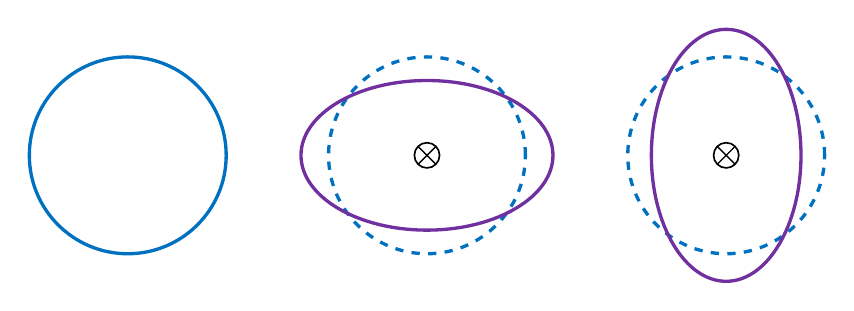
\begin{tikzpicture}

    % --- Color Definitions ---
    \definecolor{waveblue}{RGB}{0, 112, 192}
    \definecolor{wavepurple}{RGB}{112, 48, 160}

    % --- Helper Command for the Center Crosshair (\otimes) ---
    \newcommand{\crosshair}[2]{
        \draw[black, line width=0.6pt] (#1,#2) circle (0.16);
        \draw[black, line width=0.5pt] (#1,#2) ++(45:0.16) -- ++(-135:0.32);
        \draw[black, line width=0.5pt] (#1,#2) ++(135:0.16) -- ++(-45:0.32);
    }

    % ==========================================
    % 1. LEFT SHAPE: Unperturbed Circle
    % ==========================================
    \draw[waveblue, line width=1.2pt] (0,0) circle (1.25);

    % ==========================================
    % 2. MIDDLE SHAPE: Horizontally Stretched Ellipse
    % ==========================================
    % Reference dashed circle
    \draw[waveblue, line width=1.2pt, dashed] (3.8, 0) circle (1.25);
    % Stretched purple ellipse
    \draw[wavepurple, line width=1.2pt] (3.8, 0) ellipse (1.6 and 0.95);
    % Center indicator
    \crosshair{3.8}{0}

    % ==========================================
    % 3. RIGHT SHAPE: Vertically Stretched Ellipse
    % ==========================================
    % Reference dashed circle
    \draw[waveblue, line width=1.2pt, dashed] (7.6, 0) circle (1.25);
    % Stretched purple ellipse
    \draw[wavepurple, line width=1.2pt] (7.6, 0) ellipse (0.95 and 1.6);
    % Center indicator
    \crosshair{7.6}{0}

\end{tikzpicture}
\end{center}
\subsubsection*{Matter waves}
According to quantum theory, \textbf{all particles have wave properties}. The waves corresponding to particles are called matter waves. These are waves of probability: the displacement of the wave is related to the probability of finding a particle near a particular position.
\section{Wave phenomena}
\subsection{Reflection and refraction}
Wavefronts: planes will be normal to the direction of the wave.\\
Rays: lines at right angles to the wavefronts show the direction of wave propagation.
\begin{center}
  \begin{tikzpicture} [
    % Manually define the 3D projection vectors to prevent any compression
    x={(1.6cm,0cm)},      % Stretch x-axis horizontally
    y={(0cm,1.3cm)},      % Scale y-axis vertically
    z={(-0.5cm,-0.4cm)}   % Project z-axis forward and down
]

    % --- 1. Background Axes ---
    % Negative parts drawn dashed
    \draw[dashed, thin, gray] (0,0,0) -- (0,-1.3,0);
    \draw[dashed, thin, gray] (0,0,0) -- (0,0,-1.3);
    
    % Positive axes
    \draw[-{Stealth}, thick] (0,0,0) -- (0,1.8,0) node[above] {$y$};
    \draw[-{Stealth}, thick] (0,0,0) -- (0,0,2.2) node[left] {$z$};

    % --- 2. The Wave Surface (3D Ribbon) ---
    % Symmetric along the z-axis from z = -1 to z = 1
    % Wavelength is 2.2 units, crests are at x = 0.8, 3.0, 5.2
    \fill[blue!35, opacity=0.6] 
        plot[domain=0:5.8, samples=100] (\x, {0.8*cos(deg(2*pi/2.2*(\x-0.8)))}, -1)
        -- plot[domain=5.8:0, samples=100] (\x, {0.8*cos(deg(2*pi/2.2*(\x-0.8)))}, 1)
        -- cycle;

    % Sharp edge lines to define the 3D wave sheet
    \draw[blue!70!black, thick] plot[domain=0:5.8, samples=100] (\x, {0.8*cos(deg(2*pi/2.2*(\x-0.8)))}, 1);
    \draw[blue!40!black, thin, opacity=0.4] plot[domain=0:5.8, samples=100] (\x, {0.8*cos(deg(2*pi/2.2*(\x-0.8)))}, -1);

    % --- 3. The Wavefront Planes ---
    % Slicing vertically at each wave crest
    \foreach \x in {0.8, 3.0, 5.2} {
        \fill[magenta!25, opacity=0.5] (\x, -1.3, -1.3) -- (\x, 1.4, -1.3) -- (\x, 1.4, 1.3) -- (\x, -1.3, 1.3) -- cycle;
        \draw[magenta!60!black, semithick] (\x, -1.3, -1.3) -- (\x, 1.4, -1.3) -- (\x, 1.4, 1.3) -- (\x, -1.3, 1.3) -- cycle;
    }

    % --- 4. Main Ray Axis (x-axis) ---
    % Drawn through the center of the wave
    \draw[-{Stealth}, thick, blue!80!black] (0,0,0) -- (6.3,0,0) node[right, black] {$x$};
    \node[anchor=south, black] at (6.0, 0.1, 0) {ray};

    % --- 5. Annotations & Labels ---
    % "wavefronts" label with leader lines
    \node[black, anchor=south] (WF) at (1.9, 1.8, 0) {wavefronts};
    \draw[black, thin] (WF.south) -- (0.8, 1.4, 0.3);
    \draw[black, thin] (WF.south) -- (3.0, 1.4, 0.3);

    % Wavelength (lambda) markers below the wave
    \draw[{Stealth}-{Stealth}, thin] (0.8, -1.6, 0) -- (3.0, -1.6, 0) node[midway, below] {$\lambda$};
    \draw[{Stealth}-{Stealth}, thin] (3.0, -1.6, 0) -- (5.2, -1.6, 0) node[midway, below] {$\lambda$};

\end{tikzpicture}
\begin{tikzpicture}[scale=0.8]

    % --- LAYER 1: The 3D Dome (Background Hemisphere) ---
    % Rotated to match the perspective of diagram b
    \begin{scope}[rotate=65]
        % Smooth 3D-like shading for the curved outer shell of the wave
        \shade[bottom color=wave_dark!90, top color=wave_light!60] (-3,0) arc (180:0:3) -- cycle;
        % Clean outer rim definition
        \draw[wave_dark!60!black, thin] (-3,0) arc (180:0:3);
    \end{scope}

    % --- LAYER 2: The Flat Cut Face (Concentric Wavefront Rings) ---
    % Using the painter's algorithm: drawing from the largest ellipse to the smallest
    \begin{scope}[rotate=65]
        \fill[wave_dark!80] (0,0) ellipse [x radius=3.0, y radius=1.3];
        \fill[wave_med]    (0,0) ellipse [x radius=2.6, y radius=1.12];
        \fill[wave_light]  (0,0) ellipse [x radius=2.2, y radius=0.95];
        \fill[wave_dark!80] (0,0) ellipse [x radius=1.8, y radius=0.78];
        \fill[wave_med]    (0,0) ellipse [x radius=1.4, y radius=0.6];
        \fill[wave_light]  (0,0) ellipse [x radius=1.0, y radius=0.43];
        \fill[wave_dark!90] (0,0) ellipse [x radius=0.5, y radius=0.21];
        
        % Add delicate structural lines between the wavefront phases
        \foreach \r in {0.5, 1.0, 1.4, 1.8, 2.2, 2.6, 3.0} {
            \draw[wave_light!30, thin] (0,0) ellipse [x radius=\r, y radius={\r*1.3/3.0}];
        }
    \end{scope}

    % --- LAYER 3: Core Indicators & Labels ---
    % Center point source dot
    \fill[black] (0,0) circle (2.5pt);

    % "point source" label and direct leader line (placed outside rotation to stay perfectly upright)
    \node[anchor=west] (label) at (1.8, -0.8) {point source};
    \draw[-{Stealth}, thick, black] (label.west) -- (0,0);


\end{tikzpicture}
\end{center}
A point source emits waves in all directions. The wavefronts from a point source are spherical / cylindrical.
\subsubsection*{Reflection}
Law of reflection: angle of incidence = angle of reflection, $i=r$.\\
Reflection takes place when the reflecting surface is sufficiently smooth. This means that the wavelength of the incident wave has to be larger than the size of any irregularities of the surface. \\
The wavelength of the reflected waves is the same as that of the incident wave.
\begin{center}
  \begin{tikzpicture}

    % =========================================================================
    % LEFT DIAGRAM: Law of Reflection
    % =========================================================================
    \begin{scope}[xshift=0cm]
        % --- Mirror Surface ---
        \draw[thick] (-3,0) -- (3,0) node[left, at start, xshift=-4pt] {mirror};
        \foreach \x in {-2.8,-2.6,...,2.8} {
            \draw (\x,0) -- (\x-0.12,-0.12);
        }
        
        % --- Normal Line ---
        \draw[dashed, thick] (0,0) -- (0,2.6) node[above] {normal};
        \draw (0,0.2) -- (-0.2,0.2) -- (-0.2,0); % Right-angle indicator
        
        % --- Rays ---
        % Incident Ray (with arrow indicating downward direction)
        \draw[thick, raycolor] (-2.2,2.2) -- (-1.1,1.1);
        \draw[-{Stealth}, thick, raycolor] (-2.2,2.2) -- (-1.0,1.0);
        \draw[thick, raycolor] (-1.0,1.0) -- (0,0);
        
        % Reflected Ray (with arrow indicating upward direction)
        \draw[thick, raycolor] (0,0) -- (1.0,1.0);
        \draw[-{Stealth}, thick, raycolor] (0,0) -- (1.2,1.2);
        \draw[thick, raycolor] (1.2,1.2) -- (2.2,2.2);
        
        % --- Primary Labels ---
        \node[anchor=south east, inner sep=2pt] at (-2.1,2.2) {incident ray};
        \node[anchor=south west, inner sep=2pt] at (2.1,2.2) {reflected ray};
        
        % --- Angle Arcs & Values ---
        \draw (0,0.6) arc (90:135:0.6);
        \node at (-0.2,0.85) {$i$};
        
        \draw (0,0.6) arc (90:45:0.6);
        \node at (0.2,0.85) {$r$};
        
        % --- Angle Descriptions with Pointer Lines ---
        \node[anchor=south, align=center, inner sep=1pt, font=\scriptsize] (ang_inc) at (-0.7,1.4) {angle of\\incidence};
        
        \node[anchor=south, align=center, inner sep=1pt, font=\scriptsize] (ang_ref) at (0.7,1.4) {angle of\\reflection};
    \end{scope}


    % =========================================================================
    % RIGHT DIAGRAM: Image Formation in a Plane Mirror
    % =========================================================================
    \begin{scope}[xshift=7.5cm]
        % --- Mirror Surface ---
        \draw[thick] (-2,0) -- (4,0) node[left, at start, xshift=-4pt] {mirror};
        \foreach \x in {-1.8,-1.6,...,3.8} {
            \draw (\x,0) -- (\x-0.12,-0.12);
        }
        
        % --- Key Coordinates (Object & Image) ---
        \coordinate (O) at (0,2);
        \coordinate (I) at (0,-2);
        
        % Perpendicular baseline connecting Object and Image
        \draw[dashed, thick] (O) -- (I);
        
        % Object and Image Dots
        \fill[dotcolor] (O) circle (2pt) node[above right, black, xshift=-2pt] {O \enskip object};
        \fill[dotcolor] (I) circle (2pt) node[below right, black, xshift=-2pt] {I \enskip image};
        
        % Reflection Points along the Mirror
        \coordinate (M1) at (1.1,0);
        \coordinate (M2) at (1.6,0);
        \coordinate (M3) at (2.1,0);
        
        % Visible Target Endpoints for Reflected Rays
        \coordinate (E1) at (2.2, 2.0);
        \coordinate (E2) at (3.0, 2.1);
        \coordinate (E3) at (3.8, 2.2);
        
        % --- Incident Rays (Solid with mid-path directional arrows) ---
        \foreach \m in {M1, M2, M3} {
            \draw[thick, raycolor] (O) -- ($(O)!0.5!(\m)$);
            \draw[-{Stealth}, thick, raycolor] (O) -- ($(O)!0.6!(\m)$);
            \draw[thick, raycolor] ($(O)!0.6!(\m)$) -- (\m);
        }
        
        % --- Reflected Rays (Solid with forward directional arrows) ---
        \draw[thick, raycolor] (M1) -- (E1);
        \draw[-{Stealth}, thick, raycolor] (M1) -- ($(M1)!0.6!(E1)$);
        
        \draw[thick, raycolor] (M2) -- (E2);
        \draw[-{Stealth}, thick, raycolor] (M2) -- ($(M2)!0.6!(E2)$);
        
        \draw[thick, raycolor] (M3) -- (E3);
        \draw[-{Stealth}, thick, raycolor] (M3) -- ($(M3)!0.6!(E3)$);
        
        % --- Virtual Rays (Dashed extensions tracking behind the mirror) ---
        \draw[dashed, thick, raycolor] (I) -- (M1);
        \draw[dashed, thick, raycolor] (I) -- (M2);
        \draw[dashed, thick, raycolor] (I) -- (M3);
        
        % --- Schematic Eye Icon ---
        \begin{scope}[shift={(3.4,2.5)}, scale=0.55]
            % Upper and lower eyelids meeting at a point
            \draw[thick] (0.5,0.4) -- (-0.5,0) -- (0.5,-0.4);
            % Iris curve
            \draw[thick] (0.1,0.24) to[out=-115,in=115] (0.1,-0.24);
            % Shaded pupil region
            \fill (0.0,0.15) to[out=-115,in=115] (0.0,-0.15) -- (0.1,-0.15) -- (0.1,0.15) -- cycle;
            % Label
            \node[above, yshift=4pt] at (0,0.4) {eye};
        \end{scope}
        
    \end{scope}

\end{tikzpicture}
\end{center}
\subsubsection*{Refraction}
Refraction: the passage of light or any other wave from one medium into another where it has a different speed.
It changes the direction of the incident ray. The wavelength changes for the wave in the medium.
When a ray strikes an interface between two media, there is both reflection and refraction. 
\begin{itemize}
  \item If the speed of wave in medium is lower, the ray bends towards the normal.
  \item If the speed of wave in medium is higher, the ray bends away from the normal.
\end{itemize}
\subsubsection*{Snell's Law}
\[\dfrac{\sin\theta_1}{c_1}=\dfrac{\sin\theta_2}{c_2}\Rightarrow n_1\sin\theta_1=n_2\sin\theta_2\]
where $n$ is the respective refractive index (must $>1$, $\dfrac{\text{speed in vacuum}}{\text{speed in medium}}$).
\subsubsection*{Total Internal Reflection, TIR}
TIR occurs at the boundary between two media when all the incident ray in medium 1 is reflected back into medium 1. For TIR to occur, the incident material must be denser than the second material. For incident angle $>c$, no ray will be refracted and TIR would occur.\\\\
Applications of TIR include periscopes \&  \textbf{Optic fiber} (let's go CS)\\\\
When the angle of refraction is exactly 90$^\circ$ the light is refracted along the boundary. At this point, the angle of incidence is known as\textbf{ the critical angle \(c\).} Equation:
\[c=\sin^{-1}\left(\dfrac{1}{n}\right) \Leftrightarrow n=\dfrac{1}{\sin c}\]
\subsection{The principle of superposition}
想起了一些关于量子叠加态的内容...... $|k\rangle $\\
When two or more waves of the same type arrive at a given point in space at the same time, the displacement of the medium at that point is the algebraic sum of the individual displacements.
\begin{center}
  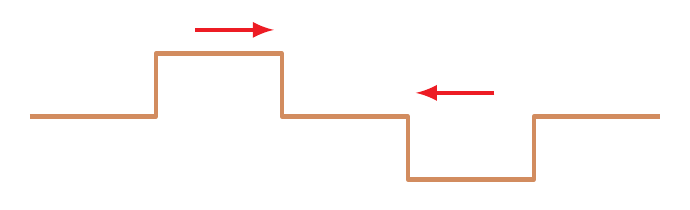
\begin{tikzpicture}
  % Color definitions matching the original image
  \definecolor{wavecolor}{RGB}{210, 140, 95}
  \definecolor{arrowcolor}{RGB}{237, 28, 36}

  % --- Subfigure a ---

  % Waveform with positive and negative rectangular pulses
  \draw[ultra thick, wavecolor, line join=round] 
    (0,4) -- (1.6,4) -- (1.6,4.8) -- (3.2,4.8) -- (3.2,4) -- 
    (4.8,4) -- (4.8,3.2) -- (6.4,3.2) -- (6.4,4) -- (8,4);
  % Directional arrows
  \draw[-latex, arrowcolor, ultra thick] (2.1, 5.1) -- (3.1, 5.1);
  \draw[-latex, arrowcolor, ultra thick] (5.9, 4.3) -- (4.9, 4.3);
\end{tikzpicture}
\end{center}
\subsubsection*{Reflection of waves}
\begin{center}
  \begin{tikzpicture}
  % Color definitions
  \definecolor{wavecolor}{RGB}{210, 140, 95}
  \definecolor{arrowcolor}{RGB}{237, 28, 36}

  % =================================================================
  % LEFT SIDE — Subfigure a: Fixed End
  % =================================================================
  
  % Top wave (approaching pulse)
  \draw[ultra thick, wavecolor] (0,5) -- (1.5,5) 
    .. controls (1.9,5) and (2.1,5.8) .. (2.5,5.8) 
    .. controls (2.9,5.8) and (3.1,5) .. (3.5,5) -- (6,5);
  \draw[-latex, arrowcolor, ultra thick] (2.1, 6.1) -- (3.1, 6.1);
  \fill[gray!70] (6, 4.3) rectangle (6.15, 5.7);
  
  % Bottom wave (reflected inverted pulse)
  \draw[ultra thick, wavecolor] (0,3) -- (1.2,3) 
    .. controls (1.6,3) and (1.8,2.2) .. (2.2,2.2) 
    .. controls (2.6,2.2) and (2.8,3) .. (3.2,3) -- (6,3);
  \draw[-latex, arrowcolor, ultra thick] (2.6, 1.8) -- (1.6, 1.8);
  \fill[gray!70] (6, 2.3) rectangle (6.15, 3.7);
  
  \node[anchor=north west, inner sep=0pt, font=\scriptsize] at (0, 1.4) {Fixed end, inverted (反作用力), phase change of 180$^\circ$};


  % =================================================================
  % RIGHT SIDE — Subfigure b: End Free to Move (Shifted X by +7.5)
  % =================================================================
  % Top wave (approaching pulse)
  \draw[ultra thick, wavecolor] (7.5,5) -- (9.0,5) 
    .. controls (9.4,5) and (9.6,5.8) .. (10.0,5.8) 
    .. controls (10.4,5.8) and (10.6,5) .. (11.0,5) -- (13.5,5);
  \draw[-latex, arrowcolor, ultra thick] (9.6, 6.1) -- (10.6, 6.1);
  
  % Rod and Ring for top setup
  \path[shading=axis, top color=gray!30, bottom color=gray!70, shading angle=90] (13.44, 4.3) rectangle (13.56, 5.7);
  \draw[ultra thick, black] (13.5, 5) ellipse (0.22 and 0.06);
  
  % Bottom wave (reflected upright pulse)
  \draw[ultra thick, wavecolor] (7.5,3) -- (8.7,3) 
    .. controls (9.1,3) and (9.3,3.8) .. (9.7,3.8) 
    .. controls (10.1,3.8) and (10.3,3) .. (10.7,3) -- (13.5,3);
  \draw[-latex, arrowcolor, ultra thick] (10.1, 1.8) -- (9.1, 1.8);
  
  % Rod and Ring for bottom setup
  \path[shading=axis, top color=gray!30, bottom color=gray!70, shading angle=90] (13.44, 2.3) rectangle (13.56, 3.7);
  \draw[ultra thick, black] (13.5, 3) ellipse (0.22 and 0.06);

  \node[anchor=north west, inner sep=0pt, font=\scriptsize] at (7.5, 1.4) {End free to move, no phase change, end falls};
  
\end{tikzpicture}
\end{center}
\subsection{Diffraction and interference}
Diffraction: The spreading of a wave as it goes past an obstacle or through an aperture.\\
Diffraction is most prominent when the wavelength $\lambda$ is larger than or equal to the gap width.
\begin{center}
  \begin{tikzpicture}[scale=0.9, line cap=round, line join=round]

    % =========================================================================
    % DIAGRAM 1: DIFFRACTION AROUND AN OBSTACLE (LEFT)
    % =========================================================================
    \begin{scope}[xshift=0cm]
        % Incoming plane waves
        \foreach \x in {0.25, 0.5, 0.75, 1.0, 1.25, 1.5, 1.75, 2.0, 2.25, 2.5, 2.75, 3.0, 3.25} {
            \draw[blue!70!cyan, thick] (\x, -2) -- (\x, 2);
        }
        
        % Direction arrow
        \draw[red, -Stealth, ultra thick] (0.5, 0) -- (2.5, 0);
        
        % Obstacle
        \draw[brown!80!black, fill=brown!40!orange!30, thick] (3.3, -0.8) rectangle (3.5, 0.8);
        
        % Diffracted waves (outgoing)
        \foreach \i in {1,...,8} {
            \pgfmathsetmacro{\r}{\i * 0.25}
            \pgfmathsetmacro{\xval}{3.5 + \r}
            % Top half wave component
            \draw[blue!70!cyan, thick] (\xval, 2) -- (\xval, 0.8) arc (0:-38:\r);
            % Bottom half wave component
            \draw[blue!70!cyan, thick] (\xval, -2) -- (\xval, -0.8) arc (0:38:\r);
        }
        
        % Label
        \node[below, text=black!80] at (2.2, -2.3) {diffraction around an obstacle};
    \end{scope}

    % =========================================================================
    % DIAGRAM 2: DIFFRACTION AT AN EDGE (MIDDLE)
    % =========================================================================
    \begin{scope}[xshift=6.5cm]
        % Incoming plane waves
        \foreach \x in {0.25, 0.5, 0.75, 1.0, 1.25, 1.5, 1.75, 2.0, 2.25, 2.5, 2.75, 3.0, 3.25} {
            \draw[blue!70!cyan, thick] (\x, -2) -- (\x, 2);
        }
        
        % Direction arrow
        \draw[red, -Stealth, ultra thick] (0.5, 0) -- (2.5, 0);
        
        % Edge Barrier
        \draw[brown!80!black, fill=brown!40!orange!30, thick] (3.3, -2) rectangle (3.5, 0);
        
        % Diffracted waves (outgoing)
        \foreach \i in {1,...,8} {
            \pgfmathsetmacro{\r}{\i * 0.25}
            \pgfmathsetmacro{\xval}{3.5 + \r}
            % Upper wave component bending past the edge
            \draw[blue!70!cyan, thick] (\xval, 2) -- (\xval, 0) arc (0:-45:\r);
        }
        
        % Label
        \node[below,text=black!80] at (2.2, -2.3) {diffraction at an edge};
    \end{scope}

    % =========================================================================
    % DIAGRAM 3: DIFFRACTION THROUGH A SLIT (RIGHT)
    % =========================================================================
    \begin{scope}[xshift=13cm]
        % Incoming plane waves (oriented upwards)
        \foreach \y in {-2.0, -1.75, -1.5, -1.25, -1.0, -0.75} {
            \draw[blue!70!cyan, thick] (1.3, \y) -- (2.1, \y);
        }
        
        % Direction arrows showing plane waves transitioning to spreading rays
        \draw[red, -Stealth, ultra thick] (1.45, -1.9) -- (1.45, -0.6);
        \draw[red, -Stealth, ultra thick] (1.70, -1.9) -- (1.70, 1.8); % Center ray
        \draw[red, -Stealth, ultra thick] (1.95, -1.9) -- (1.95, -0.6);
        
        % Spreading rays
        \draw[red, -Stealth, ultra thick] (1.70, -0.5) -- +(55:2.4);
        \draw[red, -Stealth, ultra thick] (1.70, -0.5) -- +(125:2.4);
        
        % Slit Barriers
        \draw[brown!80!black, fill=brown!40!orange!30, thick] (0.1, -0.65) rectangle (1.3, -0.5);
        \draw[brown!80!black, fill=brown!40!orange!30, thick] (2.1, -0.65) rectangle (3.3, -0.5);
        
        % Circular diffracted wavefronts out of the slit
        \foreach \i in {1,...,9} {
            \pgfmathsetmacro{\r}{\i * 0.25}
            \draw[blue!70!cyan, thick] (1.70, -0.5) ++(30:\r) arc (30:150:\r);
        }
        
        % Label
        \node[below, text=black!80] at (1.7, -2.3) {diffraction through a slit};
    \end{scope}

\end{tikzpicture}
\end{center}
\subsubsection*{Double-source interference}
When two identical waves meet at the same point in space, the principle of superposition states that the resulting wave has a displacement that is the sum of the individual displacements.
The resulting amplitude can be anything from zero to twice the amplitude of one of the waves. All waves show interference.
\begin{center}
\begin{tikzpicture}[scale=0.8, >=Stealth]

    % Configuration constants
    \def\yzero{0.8} % S1 is at (0, 0.8), S2 is at (0, -0.8)
    \def\lmb{1.1}   % Wavelength lambda

    % 1. Draw concentric wave crests from Source 1 (Green)
    \foreach \r in {1, 2, 3, 4, 5} {
        \draw[green!60!black, thick] (0, \yzero) circle (\r * \lmb);
    }

    % 2. Draw concentric wave crests from Source 2 (Blue)
    \foreach \r in {1, 2, 3, 4, 5} {
        \draw[blue!70!cyan, thick] (0, -\yzero) circle (\r * \lmb);
    }

    % 3. Draw source points S1 and S2
    \fill[green!60!black] (0, \yzero) circle (2.5pt) node[below left, text=black] {$S_1$};
    \fill[blue!70!cyan] (0, -\yzero) circle (2.5pt) node[below left, text=black] {$S_2$};

    % 4. Red Dots: Antinodal Line (Constructive Interference, path difference = 1 * lambda)
    % Dot 1: r1 = 1*lambda, r2 = 2*lambda
    \fill[red] (1.05, 1.13) circle (2.5pt);
    
    % Dot 2 (Point P): r1 = 2*lambda, r2 = 3*lambda (Crest-Crest intersection)
    \fill[red] (1.91, 1.89) circle (2.5pt) node[above left, text=black] {$P$};
    
    % Dot 3 (Point Q): r1 = 2.5*lambda, r2 = 3.5*lambda (Trough-Trough intersection)
    \fill[red] (2.33, 2.27) circle (2.5pt) node[above left, text=black] {$Q$};
    
    % Dot 4: r1 = 3*lambda, r2 = 4*lambda
    \fill[red] (2.74, 2.65) circle (2.5pt);
    
    % Dot 5: r1 = 4*lambda, r2 = 5*lambda
    \fill[red] (3.55, 3.40) circle (2.5pt);

    % 5. Black Dots: Nodal Line (Destructive Interference, path difference = 0.5 * lambda)
    % S2 is a crest (integer ring), S1 is a trough (halfway between rings)
    
    % Dot 1: r2 = 1*lambda, r1 = 0.5*lambda
    \fill[black] (0.19, 0.28) circle (2.5pt);
    
    % Dot 2: r2 = 2*lambda, r1 = 1.5*lambda
    \fill[black] (1.64, 0.66) circle (2.5pt);
    
    % Dot 3 (Point R): r2 = 3*lambda, r1 = 2.5*lambda
    \fill[black] (2.74, 1.04) circle (2.5pt) node[below right, text=black] {$R$};
    
    % Dot 4: r2 = 4*lambda, r1 = 3.5*lambda
    \fill[black] (3.80, 1.42) circle (2.5pt);
    
    % Dot 5: r2 = 5*lambda, r1 = 4.5*lambda
    \fill[black] (4.85, 1.80) circle (2.5pt);

    % 6. Path difference tracking dashed lines from sources to Point P
    \draw[dashed, black!80, thick] (0, \yzero) -- (1.91, 1.89);
    \draw[dashed, black!80, thick] (0, -\yzero) -- (1.91, 1.89);


\end{tikzpicture}
\begin{tikzpicture}[scale=0.8, >=Stealth]

    % =========================================================================
    % CONFIGURATION CONSTANTS (Sources spaced exactly 2*lambda apart)
    % =========================================================================
    \def\lmb{1.2}   % Wavelength lambda
    \def\yzero{1.2} % S1 at (0, 1.2), S2 at (0, -1.2). Separation = 2*lambda = 2.4

    % =========================================================================
    % 1. BACKGROUND WAVEFRONTS (Concentric Circles)
    % =========================================================================
    \foreach \r in {1, 2, 3, 4} {
        \draw[green!50!black, thin, opacity=0.35] (0, \yzero) circle (\r * \lmb);
        \draw[blue!60!cyan, thin, opacity=0.35] (0, -\yzero) circle (\r * \lmb);
    }

    % =========================================================================
    % 2. CENTRAL MAXIMUM (\Delta r = 0)
    % =========================================================================
    \draw[red, very thick] (-3.8, 0) -- (3.8, 0) node[right] {$\Delta r = 0$};

    % =========================================================================
    % 3. NODAL LINES (\Delta r = 0.5*lambda and 1.5*lambda) - BLACK CURVES
    % =========================================================================
    % Path difference = 0.5 * lambda (a = 0.3, b = sqrt(1.2^2 - 0.3^2) = 1.1619)
    \draw[black, very thick, domain=-3.5:3.5, samples=100] 
        plot (\x, {0.3 * sqrt(1 + (\x/1.1619)^2)}) node[right, opacity=0] {} ;
    \draw[black, very thick, domain=-3.5:3.5, samples=100] 
        plot (\x, {-0.3 * sqrt(1 + (\x/1.1619)^2)});
    
    % Labels for \Delta r = 1/2 \lambda on the left side
    \node[left] at (-3.5, 1.1) {$\Delta r = \frac{1}{2}\lambda$};
    \node[left] at (-3.5, -1.1) {$\Delta r = \frac{1}{2}\lambda$};

    % Path difference = 1.5 * lambda (a = 0.9, b = sqrt(1.2^2 - 0.9^2) = 0.7937)
    \draw[black, very thick, domain=-2.8:2.8, samples=100] 
        plot (\x, {0.9 * sqrt(1 + (\x/0.7937)^2)});
    \draw[black, very thick, domain=-2.8:2.8, samples=100] 
        plot (\x, {-0.9 * sqrt(1 + (\x/0.7937)^2)});
        
    % Labels for \Delta r = 3/2 \lambda on the left side
    \node[left] at (-2.8, 3.4) {$\Delta r = \frac{3}{2}\lambda$};
    \node[left] at (-2.8, -3.4) {$\Delta r = \frac{3}{2}\lambda$};

    % =========================================================================
    % 4. ANTINODAL LINES (\Delta r = lambda and 2*lambda) - RED CURVES
    % =========================================================================
    % Path difference = 1.0 * lambda (a = 0.6, b = sqrt(1.2^2 - 0.6^2) = 1.0392)
    \draw[red, very thick, domain=-3.2:3.2, samples=100] 
        plot (\x, {0.6 * sqrt(1 + (\x/1.0392)^2)}) node[right] {$\Delta r = \lambda$};
    \draw[red, very thick, domain=-3.2:3.2, samples=100] 
        plot (\x, {-0.6 * sqrt(1 + (\x/1.0392)^2)}) node[right] {$\Delta r = \lambda$};

    % Path difference = 2.0 * lambda (Degenerate vertical lines from sources outward)
    \draw[red, very thick] (0, \yzero) -- (0, 4.2) node[above] {$\Delta r = 2\lambda$};
    \draw[red, very thick] (0, -\yzero) -- (0, -4.2) node[below] {$\Delta r = 2\lambda$};

    % =========================================================================
    % 5. SOURCE DOTS
    % =========================================================================
    \fill[green!60!black] (0, \yzero) circle (3pt);
    \fill[blue!70!cyan] (0, -\yzero) circle (3pt);

\end{tikzpicture}
\\
$^*:$ $S_1$ and $S_2$ are identical sources.
\end{center}
The path difference: the difference in distance of the point from two sources, $\Delta r=|S_1P-S_2P|$. (For P, path difference is equivalent to $\lambda$) 
Note that at P, waves arrive as crests; at point Q, waves arrive at troughs.\\
There is \textbf{constructive interference} for the points in red and \textbf{destructive interference} for those in black.
\begin{itemize}
  \item $|S_1P-S_2P|=n\lambda$ with $n\in\mathbb{N}$ for path difference in constructive interference. It happens when two waves are in phase.
  \item $|S_1P-S_2P|=\left(n+\dfrac{1}{2}\right)\lambda$ with $n\in\mathbb{N}$ for path difference in destructive interference. Happens when two waves are \textbf{exactly} out of phase.
  \item In other cases, the resultant amplitude will be a value between 0 to $2A$.
\end{itemize}
Complete destructive interference takes place only when the two waves have equal amplitudes.
\subsubsection*{Young's Double Slit Experiment}
\begin{center}
  \begin{tikzpicture}[scale=1.3, >=Stealth]
% ==========================================
    % RIGHT COMPONENT: TOP VIEW OF DOUBLE SLIT
    % ==========================================
    \begin{scope}[shift={(0,0)}]
        \node[above, font=\small] at (1, 2.2) {top view of double slit};

        % Incoming Planar Wavefronts (Pink)
        \foreach \x in {-0.8, -0.6, ..., -0.1} {
            \draw[magenta, thick] (\x, -1) -- (\x, 1);
        }
        \node[above, font=\small] at (-0.4, 1) {$\lambda$};

        % Slit Plate with two apertures
        \filldraw[fill=orange!35!brown, draw=brown!80!black, thick] (0, -1.5) rectangle (0.1, -0.3);
        \filldraw[fill=orange!35!brown, draw=brown!80!black, thick] (0, -0.1) rectangle (0.1, 0.1);
        \filldraw[fill=orange!35!brown, draw=brown!80!black, thick] (0, 0.3) rectangle (0.1, 1.5);
        \draw[<->, black] (-0.2, -0.3) -- (-0.2, 0.3) node[midway, left] {$d$};

        % Overlapping Interfering Wavefronts (Pink Arcs)
        \foreach \r in {0.2, 0.4, ..., 2.2} {
            \draw[magenta, thin] (0.1, 0.2) ++(70:\r) arc (70:-70:\r);
            \draw[magenta, thin] (0.1, -0.2) ++(70:\r) arc (70:-70:\r);
        }

        % Geometric Envelope / Rays
        \draw[->, red, thick] (0.1, 0) -- (2.6, 0);
        \draw[->, red, thick] (0.1, 0) -- (2.6, 1.6);
        \draw[->, red, thick] (0.1, 0) -- (2.6, -1.6);
        \draw[<->, black] (0.1, -2.4) -- (2.6, -2.4) node[midway, below] {$D$};

        % Intensity Screen Target
        \filldraw[fill=black!90, draw=brown!80!black, thick] (2.6, -2) rectangle (3.2, 2);
        
        % Fringes (Alternating Magenta/Black Gradient Blocks)
        \foreach \y/\n in {1.6/4, 1.2/3, 0.8/2, 0.4/1, 0/0, -0.4/-1, -0.8/-2, -1.2/-3, -1.6/-4} {
            \fill[magenta, opacity=0.9] (2.62, \y-0.1) rectangle (3.18, \y+0.1);
            \node[right, text=black, font=\small] at (3.3, \y) {$n = \n$};
        }
        
        % Fringe Spacing Label s
        \draw[<->, white] (2.9, 0.0) -- (2.9, 0.4) node[midway, left, font=\scriptsize] {$s$};
        \node[right, font=\small, text=black, align=left] at (4.6, 0) {central\\maximum};

    \end{scope}
\end{tikzpicture}\\
\begin{tikzpicture}[scale=1.5, >=Stealth]

    % =========================================================================
    % CONFIGURATION CONSTANTS
    % =========================================================================
    \def\slitsep{1.2}  % Distance 'd' between the two slits (center-to-center)
    \def\Dlen{5.0}     % Horizontal distance 'D' to the screen
    \def\Ypos{1.6}     % Vertical position of point P on the screen

    % Coordinates
    \coordinate (Origin) at (0,0);
    \coordinate (S1) at (0, \slitsep/2);
    \coordinate (S2) at (0, -\slitsep/2);
    \coordinate (ScreenMid) at (\Dlen, 0);
    \coordinate (P) at (\Dlen, \Ypos);

    % =========================================================================
    % 1. REFERENCE LINES & RAYS
    % =========================================================================
    % Horizontal dashed reference line to the center of the screen
    \draw[dashed, thick, black!60] (Origin) -- (ScreenMid);
    
    % Central geometric ray from the slit midpoint to point P
    \draw[thick, black!90] (Origin) -- (P);
    
    % Interference path rays from Slit 1 and Slit 2 to point P
    \draw[magenta, thick] (S1) -- (P);
    \draw[magenta, thick] (S2) -- (P);

    % =========================================================================
    % 2. SLIT APERTURE WALLS (BROWN BARS)
    % =========================================================================
    \def\wallthick{3.5pt}
    \draw[orange!70!brown, line width=\wallthick] (0, \slitsep/2 + 0.15) -- (0, 1.8);
    \draw[orange!70!brown, line width=\wallthick] (0, -\slitsep/2 + 0.15) -- (0, \slitsep/2 - 0.15);
    \draw[orange!70!brown, line width=\wallthick] (0, -1.8) -- (0, -\slitsep/2 - 0.15);

    % =========================================================================
    % 3. DETECTOR SCREEN
    % =========================================================================
    \draw[ultra thick, black] (\Dlen, -1.8) -- (\Dlen, 2.0);
    \node[right, black, font=\bfseries] at (P) {P};

    % =========================================================================
    % 4. ANGULAR ARC (\theta)
    % =========================================================================
    % Calculate angle dynamically for accuracy
    \pgfmathsetmacro{\thetaAngle}{atan(\Ypos/\Dlen)}
    \draw[black, thin] (0.9, 0) arc (0:\thetaAngle:0.9);
    \node[black, font=\small] at ({\thetaAngle/2}:0.7) {$\theta$};

    % =========================================================================
    % 5. DIMENSIONS & LABELS
    % =========================================================================
    % Slit separation 'd'
    \draw[<->, black] (-0.25, -\slitsep/2) -- (-0.25, \slitsep/2) node[midway, left=-1pt] {$d$};
    \draw[black, thin] (-0.3, \slitsep/2) -- (-0.15, \slitsep/2);
    \draw[black, thin] (-0.3, -\slitsep/2) -- (-0.15, -\slitsep/2);

    % Fringe displacement 's_n'
    \draw[<->, black] (\Dlen + 0.2, 0) -- (\Dlen + 0.2, \Ypos) node[midway, right=-1pt] {$s_n$};
    \draw[black, thin] (\Dlen + 0.15, \Ypos) -- (\Dlen + 0.3, \Ypos);
    \draw[black, thin] (\Dlen + 0.15, 0) -- (\Dlen + 0.3, 0);

    % Screen distance 'D' and Center label
    \node[below, black] at (\Dlen*0.45, -0.05) {$D$};
    \node[below, black] at (\Dlen*0.75, -0.05) {center of screen};

\end{tikzpicture}
\begin{tikzpicture}[scale=1.3,>=Stealth]

    % =========================================================================
    % CONFIGURATION CONSTANTS
    % =========================================================================
    \def\d{2.5}      % Distance between slits S1 and S2
    \def\ang{22}     % Angle theta of the diffracted rays
    \def\raylen{4.5} % Length of the rays

    % Coordinates for Slits and Origin
    \coordinate (Origin) at (0,0);
    \coordinate (S1) at (0, \d/2);
    \coordinate (S2) at (0, -\d/2);

    % Calculate exact position of point Z on the lower ray using vector projection
    % Z = S2 + (d * sin(theta)) in the direction of the ray
    \coordinate (Z) at ($(S2) + (\ang:{\d * sin(\ang)})$);

    % =========================================================================
    % 1. VERTICAL SLIT PLATE (BROWN BARS)
    % =========================================================================
    \draw[orange!70!brown, line width=3.5pt] (0, \d/2 + 0.15) -- (0, 2.2);
    \draw[orange!70!brown, line width=3.5pt] (0, -\d/2 + 0.15) -- (0, \d/2 - 0.15);
    \draw[orange!70!brown, line width=3.5pt] (0, -2.2) -- (0, -\d/2 - 0.15);

    % Source Labels
    \node[left, xshift=-2pt, yshift=8 pt] at (S1) {$S_1$};
    \node[left, xshift=-2pt, yshift=-8pt] at (S2) {$S_2$};

    % =========================================================================
    % 2. PROPAGATING RAYS (MAGENTA LINES WITH MID-ARROWS)
    % =========================================================================
    % Upper Ray from S1
    \draw[magenta, very thick] (S1) -- ++(\ang:\raylen*0.4) coordinate (A1);
    \draw[magenta, very thick, ->] (A1) -- ++(\ang:0.1);
    \draw[magenta, very thick] (A1) -- ++(\ang:\raylen*0.6);

    % Lower Ray from S2
    \draw[magenta, very thick] (S2) -- ++(\ang:\raylen*0.4) coordinate (A2);
    \draw[magenta, very thick, ->] (A2) -- ++(\ang:0.1);
    \draw[magenta, very thick] (A2) -- ++(\ang:\raylen*0.6);

    % =========================================================================
    % 3. REFERENCE DASHED LINES
    % =========================================================================
    % Central line pointing "to P"
    \draw[dashed, thick, black!80] (Origin) -- ++(\ang:\raylen) node[above left, black] {to P};
    
    % Horizontal reference line to center of screen
    \draw[dashed, thick, black!70] (Origin) -- (\raylen, 0) node[below, black, yshift=-2pt] {center of screen};

    % =========================================================================
    % 4. GEOMETRIC PERPENDICULAR & RIGHT ANGLES
    % =========================================================================
    % Perpendicular line S1 to Z
    \draw[black, thick] (S1) -- (Z) node[below right, yshift=-2pt, xshift=-2pt] {Z};

    % Right angle square at Z
    \draw[black, thin] (Z) -- ++(\ang+90:0.2) -- ++(\ang+180:0.2) -- ++(\ang+90:-0.2);

    % Right angle square at S1
    \draw[black, thin] (S1) -- ++(\ang:0.2) -- ++(\ang-90:0.2) -- ++(\ang:-0.2);

    % =========================================================================
    % 5. ANGULAR LABELS (\theta)
    % =========================================================================
    % Theta 1: Between horizontal and central dashed line
    \draw[black, thin] (0.9, 0) arc (0:\ang:0.9);
    \node[black, font=\small] at ({\ang/2}:1.15) {$\theta$};

    % Theta 2: Between vertical slit plate and perpendicular line S1-Z
    \draw[black, thin] (S1) ++(-90:0.5) arc (-90:-90+\ang:0.5);
    \node[black, font=\small] at ($(S1) + (-90+\ang/2:0.75)$) {$\theta$};

    % =========================================================================
    % 6. SLIT SEPARATION DIMENSION (d)
    % =========================================================================
    \draw[black, thin] (-0.15, \d/2) -- (-0.45, \d/2);
    \draw[black, thin] (-0.15, -\d/2) -- (-0.45, -\d/2);
    \draw[<->, black, thick] (-0.35, -\d/2) -- (-0.35, \d/2) node[midway, fill=white, inner sep=2pt] {$d$};

\end{tikzpicture}\\
The value of $n$ indicates that the path difference is $n\lambda$.
\end{center}
Here, the path difference is $S_2Z=d\sin\theta$.\\
Deduction process for the linear separation on a screen of two consecutive maxima, $s$:
\begin{itemize}
  \item Because $d$ is small, $\sin\theta\approx\tan\theta\approx\theta$.
  \item From left diagram, $\tan\theta=\dfrac{s_n}{D}\Rightarrow s_n=D\sin\theta$
  \item $\sin\theta=\dfrac{n\lambda}{d}\Rightarrow s_n=\dfrac{n\lambda D}{d}$
  \item $s=\dfrac{\lambda D}{d}$, the maxima of the interference pattern are equally separated.
\end{itemize}
Coherent waves: phase difference between two waves (originated from the same source) does not change with time.\\\\
An intensity of one unit corresponds to the intensity from only one slit. At points of constructive interference the amplitude is double that of just one wave. Since intensity is proportional to the square of the amplitude, the intensity is four times as large.
\newpage
\subsection{Single-slit diffraction}
Diffraction is negligible is $\lambda$ is much smaller than the gap width and obvious when $\lambda\geq$ gap width.

\begin{center}
  \begin{tikzpicture}[>=Stealth, scale=0.9]

    % Define Styles
    \tikzstyle{ray} = [line width=1.2pt, color=magenta, ->-/.style={decoration={markings, mark=at position 0.5 with {\arrow{>}}}, postaction={decorate}}]
    
    % Slit Boundaries (Grey Blocks)
    \fill[gray!80!black] (-0.3, 4.5) -- (0, 4.5) -- (0, 3.5) -- (-0.3, 3.5) -- cycle;
    \fill[gray!80!black] (-0.3, -4.5) -- (0, -4.5) -- (0, -3.5) -- (-0.15, -3.8) -- (-0.3, -3.8) -- cycle;

    % Slit line (Pink vertical line)
    \draw[line width=1.5pt, color=magenta] (0,-3.5) -- (0,3.5);
    
    % Dimension 'b'
    \draw[<->, shift={(-1,0)}] (0,-3.5) -- (0,3.5) node[midway, fill=white] {$b$};
    % Point coordinates along the slit
    % Total height = 7 units (from -3.5 to 3.5)
    % A1 is at 3.5. B1 is at 0.
    % Top half divided into 5 segments? The diagram shows A1 to A5, then B1 to B5.
    % Let's place them evenly. Center line is at 0.
    % A1=3.5, A2=2.8, A3=2.1, A4=1.4, A5=0.7
    % B1=0, B2=-0.7, B3=-1.4, B4=-2.1, B5=-2.8
    
    \coordinate (A1) at (0, 3.5);
    \coordinate (A2) at (0, 2.8);
    \coordinate (A3) at (0, 2.1);
    \coordinate (A4) at (0, 1.4);
    \coordinate (A5) at (0, 0.7);
    \coordinate (B1) at (0, 0);
    \coordinate (B2) at (0, -0.7);
    \coordinate (B3) at (0, -1.4);
    \coordinate (B4) at (0, -2.1);
    \coordinate (B5) at (0, -2.8);

    % Draw dots and labels
    \foreach \p/\label/\pos in {A1/$A_1$/left, A2/$A_2$/left, A3/$A_3$/left, A4/$A_4$/left, A5/$A_5$/left, B1/$B_1$/left, B2/$B_2$/left, B3/$B_3$/left, B4/$B_4$/left, B5/$B_5$/left} {
        \fill (\p) circle (1.2pt);
        \node[\pos, xshift=-1pt, font=\small] at (\p) {\label};
    }

    % Center line of slit
    \draw[dashed, line width=0.6pt] (B1) -- (5,0) node[right, yshift=-2pt, font=\small] {center line of slit};

    % Ray angles and directions
    % Let angle \theta = 22 degrees
    \def\thetaValue{22}
    \coordinate (C1) at ({3.5*sin(\thetaValue)*cos(\thetaValue)}, {3.5*sin(\thetaValue)*sin(\thetaValue)});
    
    % Draw Rays (magenta lines with arrows)
    \draw[line width=1.2pt, color=magenta] (A1) -- ++(\thetaValue:4.5);
    \draw[line width=1.2pt, color=magenta, ->] (A1) -- ++(\thetaValue:2.5);
    
    \draw[line width=1.2pt, color=magenta] (B1) -- ++(\thetaValue:6.5);
    \draw[line width=1.2pt, color=magenta, ->] (B1) -- ++(\thetaValue:4.5);

    % Draw Wavefront line A1 to C1
    \draw[line width=0.8pt, black] (A1) -- (C1);
    \node[right, xshift=1pt, yshift=10pt] at (C1) {$C_1$};

    % Right angle symbol at C1
    \begin{scope}[rotate=\thetaValue]
        \draw[thin] ($(C1)+(-0.25,0)$) -- ($(C1)+(-0.25,0.25)$) -- ($(C1)+(0,0.25)$);
    \end{scope}

    % Text pointer for "to point P on distant screen"
    \node[anchor=west, align=left, font=\small] at (4,3.2) {to point P on\\distant screen};
    
    % Large arrow indicating general direction
    \draw[line width=1.5pt, ->] (2.2, 1.8) -- ++(\thetaValue:1.2);

    % Path difference labels and arrows
    \draw[<->] ($(B1)+(0.05, -0.15)$) -- ($(C1)+(0.05, -0.15)$) node[midway, below, yshift=-2pt, xshift=6pt, align=center, font=\small] {path\\difference};

    % Angles (\theta)
    % Angle at A1: between vertical line (downwards) and A1-C1
    % Vertical down from A1 is along the pink line towards B1.
    % So angle is B1 - A1 - C1.
    \coordinate (DownA1) at (0, 1);
    
    \pic [draw, -, angle radius=18pt, "$\theta$", angle eccentricity=1.4] {angle = B1--A1--C1};

    % Angle at B1: between dashed horizontal line and ray
    \coordinate (EastB1) at (2, 0);
    
    \pic [draw, -, angle radius=22pt, "$\theta$", angle eccentricity=1.3] {angle = EastB1--B1--C1};
\end{tikzpicture}\\
Points from $A_1$ to $A_5$ and from $B_1$ to $B_5$ are in phase (lies on the same wavefront). \\The results of the interference of the waves can be seen on a distant screen.
\end{center}
The path difference between ray $A_1$ and $B_1$ is equal to $B_1C_1=\dfrac{b}{2}\sin\theta$. This would result in complete destructive interference if the path difference is half of the wavelength. $\dfrac{b}{2}\sin\theta=\dfrac{\lambda}{2}\Rightarrow b\sin\theta=\lambda$\\
For every point on the upper half of the slit there is a corresponding point on the lower half, so we see that all the points on the wavefront will result in complete destructive interference if the first pair results in destructive interference.\\
Approximate formula for the angle of the first diffraction minimum: $\theta=\dfrac{\lambda}{b}$, where $b$ is the slit width.
\begin{center}
  \begin{tikzpicture}[>=Stealth]

    % Define dimensions and grid limits
    % x-axis: -0.12 to 0.12. Let 1 unit on x = 40mm -> -0.12 is -4.8, 0.12 is 4.8
    % Grid lines every 0.01 on x -> 0.01 * 40 = 0.4cm = 4mm
    % y-axis: 0 to 1.1. Let 1 unit on y = 4.0cm -> 1.0 is 4.0cm, 0.1 is 4mm
    
    \def\xscale{40}
    \def\yscale{4}

    % 1. Draw Background Grid (Light Blue)
    % x ranges from -0.11 to 0.12 in steps of 0.01
    % y ranges from 0 to 1.1 in steps of 0.1
    \draw[xstep={0.01*\xscale}, ystep={0.1*\yscale}, color=blue!20!white, line width=0.5pt] 
        (-0.11*\xscale, 0) grid (0.12*\xscale, 1.1*\yscale);

    % 2. Draw Axes
    \draw[line width=1.0pt, color=gray!80!black] (-0.11*\xscale, 0) -- (0.12*\xscale, 0) node[right, black] {$\theta/\rm{rad}$};
    \draw[line width=1.0pt, color=gray!80!black] (0, -0.1) -- (0, 1.1*\yscale);

    % Axis Labels & Ticks
    % y-axis ticks
    \foreach \y in {0.2, 0.4, 0.6, 0.8, 1.0} {
        \draw[line width=0.8pt] (-2pt, \y*\yscale) -- (2pt, \y*\yscale);
        \node[left, font=\small, xshift=-1pt] at (0, \y*\yscale) {\pgfmathprintnumber[fixed, precision=1]{\y}};
    }
    \node[above, font=\small, yshift=2pt] at (0, 1.1*\yscale) {Intensity};

    % x-axis ticks
    \foreach \x in {-0.10, -0.05, 0.00, 0.05, 0.10} {
        \draw[line width=0.8pt] (\x*\xscale, -2pt) -- (\x*\xscale, 2pt);
        \node[below, font=\small, yshift=-2pt] at (\x*\xscale, 0) {\pgfmathprintnumber[fixed, precision=2]{\x}};
    }

    % 3. Draw Intensity Curve (Single Slit Diffraction Pattern)
    % Intensity I(\theta) = I_0 * [sin(\alpha) / \alpha]^2
    % where \alpha = \pi * b * sin(\theta) / \lambda
    % From the graph, first minimum is at \theta = 0.05 rad.
    % Since first minimum is at \theta = \lambda / b, we can set b/\lambda = 1 / 0.05 = 20.
    % So \alpha = 20 * \pi * \theta.
    % We use a high sample plot within gnuplot-like syntax natively in TikZ math engine.
    
    \draw[color=red!90!black, line width=1.2pt, samples=200, domain=-0.11:0.12]
        plot (\x*\xscale, { \yscale * (\x == 0 ? 1.0 : (sin(20*\x*180)/ (20*\x*pi) )^2) });

    % 4. Labels and Pointers
    % Central Maximum Arrow
    \draw[<-] (0.01*\xscale, 1.02*\yscale) -- (0.04*\xscale, 0.9*\yscale) 
        node[right, font=\small, yshift=-2pt] {central maximum};

    % First Minimum Arrow
    \draw[<-] (0.052*\xscale, 0.02*\yscale) -- (0.057*\xscale, 0.15*\yscale) 
        node[above, font=\small, xshift=15pt, yshift=-2pt] {first minimum};

    % Secondary Maximum Arrow
    \draw[<-] (-0.072*\xscale, 0.05*\yscale) -- (-0.075*\xscale, 0.15*\yscale) 
        node[above, font=\small, align=center, yshift=-2pt] {secondary\\maximum};

    % 5. Green Double-Headed Arrow at the bottom
    \draw[<->, color=green!60!black, line width=0.8pt,yshift=-6pt] (-0.05*\xscale, -0.4) -- (0.05*\xscale, -0.4);

\end{tikzpicture}
\\
Intensity in single slit diffraction for red light. 
\end{center}
The intensity of the first secondary maximum is only about 4.5\% of the intensity at the central maximum.\\
The angular width of the central maximum (measured by the green arrow) is given by $\dfrac{2\lambda}{b}$.\\
If we increase the slit width, more light goes through so the intensity will increase and the angular width will decrease.\\
Blue light has a shorter wavelength and so with blue light the first minimum occurs at smaller angle.
\newpage
\subsubsection*{Effect of (non-negligible) slit width on two-slit intensity patterns}
The single slit diffraction pattern modulates the two-slit pattern so that the intensity is given by the blue curve. The effect of the slit width is that the red curve becomes the envelope of the blue curve.
\begin{center}
  \begin{tikzpicture}[>=Stealth]

    % Define scaling factors
    % x-axis: -30 to 30 degrees. Let 1 unit on x = 0.16cm -> 30 units = 4.8cm
    % Grid lines every 2 degrees -> 2 * 0.16 = 0.32cm
    % y-axis: 0 to 4.2. Let 1 unit on y = 1.0cm -> 4.0 is 4.0cm
    
    \def\xscale{0.16}
    \def\yscale{1.0}

    % 1. Draw Background Grid (Light Blue)
    % x ranges from -30 to 30 in steps of 2
    % y ranges from 0 to 4.2 in steps of 0.2
    \draw[xstep={2*\xscale}, ystep={0.2*\yscale}, color=blue!20!white, line width=0.5pt] 
        (-30*\xscale, 0) grid (30*\xscale, 4.2*\yscale);

    % 2. Draw Axes
    \draw[line width=1.0pt, color=gray!80!black] (-30*\xscale, 0) -- (30*\xscale, 0) node[right, black, xshift=2pt] {degrees};
    \draw[line width=1.0pt, color=gray!80!black] (0, 0) -- (0, 4.3*\yscale);

    % Axis Labels & Ticks
    % y-axis labels and ticks
    \foreach \y in {1, 2, 3, 4} {
        \draw[line width=0.8pt] (-2pt, \y*\yscale) -- (2pt, \y*\yscale);
        \node[left, font=\small, xshift=-1pt] at (0, \y*\yscale) {\y};
    }
    \node[above, font=\small] at (0, 4.3*\yscale) {$I/I_0$};

    % x-axis labels and ticks
    \foreach \x in {-30, -20, -10, 0, 10, 20, 30} {
        \draw[line width=0.8pt] (\x*\xscale, -2pt) -- (\x*\xscale, 2pt);
        \node[below, font=\small, yshift=-3pt] at (\x*\xscale, 0) {\x};
    }

    % 3. Draw Modulation Envelope and Interference Pattern
    % This represents a double-slit interference pattern modulated by a single-slit diffraction envelope.
    % Envelope (Red): I_env = 4 * [sin(\alpha) / \alpha]^2
    % From graph, first diffraction minimum is at roughly \pm 18 degrees.
    % Interference (Blue): I = I_env * cos(\beta)^2
    % From graph, interference peaks occur at 0, \pm 7, \pm 14 degrees.

    % Red Curve (Single Slit Diffraction Envelope)
    \draw[color=red!90!black, line width=1.1pt, samples=300, domain=-30:30]
        plot (\x*\xscale, { 4.0*\yscale * (\x == 0 ? 1.0 : (sin(\x*180/18)/ (\x*pi/18) )^2) });

    % Blue Curve (Double Slit Interference Pattern)
    \draw[color=blue!80!black, line width=1.1pt, samples=400, domain=-30:30]
        plot (\x*\xscale, { 4.0*\yscale * (\x == 0 ? 1.0 : (sin(\x*180/18)/ (\x*pi/18) )^2) * (cos(\x*180/7))^2 });

\end{tikzpicture}
\end{center}
\subsection{Multiple slits}
As the number of slits increases, the interference pattern increases in complexity. 
With $N$ slits, there are $N-2$ secondary maxima. The intensity of the central maximum is $N^2$ times the intensity of just one slit by itself.\\
As the number of slits increases:
\begin{itemize}
  \item The primary maxima are observed at the same angles
  \item The primary maxima get narrower and brighter
  \item The secondary maxima become unimportant
\end{itemize}
\begin{center}
  \begin{tikzpicture}[>=Stealth]

    % Define scaling factors
    % x-axis: -30 to 30 degrees. Let 1 unit on x = 0.16cm -> 30 units = 4.8cm
    % Grid lines every 2 degrees -> 2 * 0.16 = 0.32cm
    % y-axis: 0 to 16.5. Let 1 unit on y = 0.25cm -> 16 is 4.0cm
    
    \def\xscale{0.16}
    \def\yscale{0.25}

    % 1. Draw Background Grid (Light Blue)
    % x ranges from -30 to 30 in steps of 2
    % y ranges from 0 to 16.5 in steps of 1
    \draw[xstep={2*\xscale}, ystep={1*\yscale}, color=blue!20!white, line width=0.5pt] 
        (-30*\xscale, 0) grid (30*\xscale, 16.5*\yscale);

    % 2. Draw Axes
    \draw[line width=1.0pt, color=gray!80!black] (-30*\xscale, 0) -- (30*\xscale, 0) node[below right, black, xshift=-10pt, yshift=-13pt] {$\theta$/degrees};
    \draw[line width=1.0pt, color=gray!80!black] (0, 0) -- (0, 16.6*\yscale);

    % Axis Labels & Ticks
    % y-axis labels and ticks
    \foreach \y in {5, 10, 15} {
        \draw[line width=0.8pt] (-2pt, \y*\yscale) -- (2pt, \y*\yscale);
        \node[left, font=\small, xshift=-1pt] at (0, \y*\yscale) {\y};
    }
    \node[above, font=\small] at (0, 16.6*\yscale) {Intensity};

    % x-axis labels and ticks
    \foreach \x in {-30, -20, -10, 0, 10, 20, 30} {
        \draw[line width=0.8pt] (\x*\xscale, -2pt) -- (\x*\xscale, 2pt);
        \node[below, font=\small, yshift=-3pt] at (\x*\xscale, 0) {\x};
    }

    % 3. Draw Modulation Envelope and N-Slit Interference Pattern
    % We scale the domain coordinates safely to prevent PGF math overflow.

    % Red Curve (N=4 Slit Pattern)
    \draw[color=red!90!black, line width=1.1pt, samples=600, domain=-30:30]
        plot (\x*\xscale, { 
            16.0*\yscale * (\x == 0 ? 1.0 : (sin(12*\x) / (\x*pi/15))^2) *
            (\x == 0 ? 1.0 : (sin(4*26.5*\x) / (4*sin(26.5*\x)))^2)
        });

    % Blue Curve (Modulation Envelope)
    \draw[color=blue!80!black, line width=1.1pt, samples=300, domain=-30:30]
        plot (\x*\xscale, { 
            16.0*\yscale * (\x == 0 ? 1.0 : (sin(12*\x) / (\x*pi/15))^2)
        });
    % 4. Labels and Pointers
    % "primary maxima" label and arrows
    \node[anchor=west, font=\small] at (5*\xscale, 10*\yscale) {primary maxima};

    % "two secondary maxima" label and arrow
    \node[anchor=north, align=center, font=\small, yshift=-8pt] at (0, -1*\yscale) {two secondary\\maxima};

\end{tikzpicture}
\end{center}
\subsubsection*{Diffraction Grating}
Used to measure wavelength of light.
A diffraction grating consists of a large number of parallel slits of very small width.
(Instead of actual slits, modern gratings consist of a transparent slide on which rulings or grooves have been precisely cut.)
The maxima in the interference pattern are sharp and bright and can easily be distinguished from their neighbours, they are called "lines".
\begin{center}
  \begin{tikzpicture}[>=Stealth,scale=0.9]

    % Define scaling factors
    % x-axis: let 1 unit = 1cm. Total range from -4.5 to 5.5
    % y-axis: max peak height is 4.0cm
    \def\xscale{1.0}
    \def\yscale{1}

    % 1. Draw Axes with arrows
    \draw[line width=0.8pt, ->] (-4.5*\xscale, 0) -- (4.5*\xscale, 0) node[below right, black] {$\theta/\rm{degrees}$};
    \draw[line width=0.8pt, ->] (0, 0) -- (0, 4.7*\yscale) node[above, black] {Intensity};

    % 2. Draw Diffraction Grating Sharp Peaks
    % This pattern represents many slits (a diffraction grating), which creates 
    % very sharp, narrow maxima separated by flat regions of near-zero intensity.
    % Using a high power of a cosine function: I(\theta) = \cos^2( \frac{\pi \cdot \theta}{d} )^N
    % Peaks are evenly spaced at x = -3, -1.5, 0, 1.5, 3, 4.5
    \draw[color=blue!80!black, line width=1.1pt, samples=600, domain=-4.2:4.2]
        plot (\x*\xscale, { 4.5 * (cos(\x * 120))^32 });

\end{tikzpicture}
\begin{tikzpicture}[>=Stealth]

    % --- Left Pink Large Arrow (Incoming Light) ---
    \fill[pink!40] (-3,1) -- (-2.3,1) -- (-2.3,2.2) -- (-1.1,0) -- (-2.3,-2.2) -- (-2.3,-1) -- (-3,-1) -- cycle;
    \node at (-2.1,0) [font=\large\bfseries, text=black!80] {light};

    % --- Diffraction Grating (Vertical dashed/slitted lines) ---
    \coordinate (Gtop) at (-0.5, 2.5);
    \coordinate (Gbot) at (-0.5,-2.5);
    
    % Draw the grating bars
    \foreach \y in {2.2, 1.2, 0.2, -0.8, -1.8} {
        \draw[brown!70!black, line width=3pt] (-0.5, \y) -- (-0.5, \y-0.9);
    }
    \node at (-0.4, 2.5) [anchor=south] {diffraction grating};

    % --- Slit positions (sources of light rays) ---
    \coordinate (S0) at (-0.5, 1.2);
    \coordinate (S1) at (-0.5, 0.2);
    \coordinate (S2) at (-0.5, -0.8);
    \coordinate (S3) at (-0.5, -1.8);
    \coordinate (S4) at (-0.5, -2.8);

    % --- Horizontal reference line from center-ish slit ---
    \draw[dashed, thick, black!70] (S2) -- (4.5, -0.8);

    % --- Angled Rays (Magenta) ---
    \def\angletheta{20}
    \def\raylen{5.0}
    
    % Draw the parallel outgoing rays
    \draw[magenta, thick, ->] (S0) -- +(\angletheta:\raylen-0.5);
    \draw[magenta, thick, ->] (S1) -- +(\angletheta:\raylen);
    \draw[magenta, thick, ->] (S2) -- +(\angletheta:\raylen+0.5);
    \draw[magenta, thick, ->] (S3) -- +(\angletheta:\raylen+1.0);
    \draw[magenta, thick, ->] (S4) -- +(\angletheta:\raylen+1.5);

    % --- Wavefront Line (Dashed Magenta Line, perpendicular to rays) ---
    % Normal vector to angletheta is \angletheta + 90 or -90. 
    % Let's drop a perpendicular wavefront from S0 to the bottom ray.
    % The distance from slit to wavefront along the ray is d*sin(theta)
    % Let d = 1.0 (distance between slits)
    \def\d{1.0}
    \coordinate (W0) at (S0);
    \coordinate (W1) at ($(S1) + (\angletheta:{\d*sin(\angletheta)})$);
    \coordinate (W2) at ($(S2) + (\angletheta:{2*\d*sin(\angletheta)})$);
    \coordinate (W3) at ($(S3) + (\angletheta:{3*\d*sin(\angletheta)})$);
    \coordinate (W4) at ($(S4) + (\angletheta:{4*\d*sin(\angletheta)})$);

    \draw[magenta, dashed, thick] (W0) -- (W4);

    % --- Path Difference Segments (Blue Lines) ---
    \draw[cyan!80!blue, thick] (S1) -- (W1);
    \draw[cyan!80!blue, thick] (S2) -- (W2);
    \draw[cyan!80!blue, thick] (S3) -- (W3);
    \draw[cyan!80!blue, thick] (S4) -- (W4);

    % --- Labels for Path Differences (\delta, 2\delta, etc.) ---
    \node at ($(S1)!0.5!(W1)$) [anchor=south west, inner sep=1pt, font=\small, xshift=-5pt, yshift=2pt] {$\delta$};
    \node at ($(S2)!0.5!(W2)$) [anchor=south west, inner sep=1pt, font=\small, xshift=-5pt, yshift=2pt] {$2\delta$};
    \node at ($(S3)!0.5!(W3)$) [anchor=south west, inner sep=1pt, font=\small, xshift=-5pt, yshift=2pt] {$3\delta$};
    \node at ($(S4)!0.5!(W4)$) [anchor=south west, inner sep=1pt, font=\small, xshift=-5pt, yshift=2pt] {$4\delta$};

    % --- Right Angle Indicator at the first path difference ---
    \path (S1) -- (W1) coordinate[pos=1] (W1_pt);
    \draw[black!60] ($(W1_pt)!0.12!(S1)$) -- ($($(W1_pt)!0.12!(S1)$)+(\angletheta+90:0.12)$) -- ($(W1_pt)+(\angletheta+90:0.12)$);

    % 2. Angle relative to the horizontal dashed line
    \coordinate (RefEnd) at (1.5, -0.8);
    \coordinate (RayEnd) at ($(S2) + (\angletheta:2.0)$);
    
    \draw[black] ($(S2) + (0:0.8)$) arc[start angle=0, end angle=\angletheta, radius=0.8];
    \node at ($(S2) + (\angletheta/2:1.1)$) {$\theta$};

\end{tikzpicture}
  \\
  The intensity distribution of diffraction grating. \\The maxima have roughly the same intensity and are very narrow.\\
  右图中$\delta=d\sin\theta$即为path difference.
\end{center}
The maxima of the pattern are observed at angles that can be found by:
\[d\sin\theta=n\lambda, n\in\mathbb{Z}\]
A maximum observed at $n=k$ is called the $k^\text{th}$ order maximum.\\
In practice, "$x$ lines per mm" $\Leftrightarrow$ $d=\dfrac{1}{x}$ mm.\\\\
White light incidence on diffraction grating:
\begin{center}
\begin{tikzpicture}[
    scale=0.7,
    ray/.style={thick, -latex, shorten >=0.5pt},
    red ray/.style={ray, red},
    green ray/.style={ray, green!70!black},
    blue ray/.style={ray, blue},
    white ray/.style={ray, black},
    label node/.style={anchor=west, font=\large}
]

    % Define common coordinates and lengths
    \def\L{6.0}   % Distance from grating to screen
    \def\gratingX{0}
    \def\screenX{\L}
    \def\startY{0}

    % Central start point
    \coordinate (start) at (\gratingX, \startY);
    
    % --- Left Side Elements (Incident Light and Grating) ---
    % Incoming arrow
    \draw[ray, thick] (-2, \startY) -- (-0.2, \startY);
    
    % "white light" text
    \node[anchor=south west] at (-2.3, 0.2) [align=left] {white\\light};
    
    % "diffraction grating" text and line
    \draw[ultra thick] (\gratingX, 0.5) -- (\gratingX, -0.5);
    \node[anchor=north east] at (-0.2, -0.4) [align=right] {diffraction\\grating};

    % --- Right Side Elements (Screen) ---
    % Vertical line for the screen
    \draw[thick] (\screenX, -5) -- (\screenX, 5);

    % Central ray n=0 (representing white)
    \draw[white ray] (start) -- (\screenX, \startY) node[label node, xshift=3pt] {$n=0$ (white)};

    % --- Diffracted Rays Configuration ---
    % Renamed macros cleanly to avoid parsing errors
    \def\thetaRone{18}
    \def\thetaGone{15}
    \def\thetaBone{12}
    
    \def\thetaRtwo{38}
    \def\thetaGtwo{32}
    \def\thetaBtwo{26}

    % Define end points for n=1 and n=-1
    \coordinate (endR1p) at (\screenX, {\L * tan(\thetaRone)});
    \coordinate (endG1p) at (\screenX, {\L * tan(\thetaGone)});
    \coordinate (endB1p) at (\screenX, {\L * tan(\thetaBone)});

    \coordinate (endR1n) at (\screenX, {-\L * tan(\thetaRone)});
    \coordinate (endG1n) at (\screenX, {-\L * tan(\thetaGone)});
    \coordinate (endB1n) at (\screenX, {-\L * tan(\thetaBone)});
    
    % Define end points for n=2 and n=-2
    \coordinate (endR2p) at (\screenX, {\L * tan(\thetaRtwo)});
    \coordinate (endG2p) at (\screenX, {\L * tan(\thetaGtwo)});
    \coordinate (endB2p) at (\screenX, {\L * tan(\thetaBtwo)});

    \coordinate (endR2n) at (\screenX, {-\L * tan(\thetaRtwo)});
    \coordinate (endG2n) at (\screenX, {-\L * tan(\thetaGtwo)});
    \coordinate (endB2n) at (\screenX, {-\L * tan(\thetaBtwo)});

    % --- Drawing the Rays ---

    % n=2 orders
    \draw[red ray] (start) -- (endR2p);
    \draw[green ray] (start) -- (endG2p);
    \draw[blue ray] (start) -- (endB2p);
    \node[label node, xshift=3pt] at (endG2p) {$n=2$};

    % n=-2 orders
    \draw[blue ray] (start) -- (endB2n);
    \draw[green ray] (start) -- (endG2n);
    \draw[red ray] (start) -- (endR2n);
    \node[label node, xshift=3pt] at (endG2n) {$n=-2$};

    % n=1 orders
    \draw[red ray] (start) -- (endR1p);
    \draw[green ray] (start) -- (endG1p);
    \draw[blue ray] (start) -- (endB1p);
    \node[label node, xshift=3pt] at (endG1p) {$n=1$};

    % n=-1 orders
    \draw[blue ray] (start) -- (endB1n);
    \draw[green ray] (start) -- (endG1n);
    \draw[red ray] (start) -- (endR1n);
    \node[label node, xshift=3pt] at (endG1n) {$n=-1$};

\end{tikzpicture}
\end{center}
The $n = 1$ and $n = 2$ orders are beginning to overlap. This is because different wavelengths in different orders can satisfy the grating equation at the same angle, so light from the second order falls on top of light from the first order.
\section{Standing waves and resonance}
\subsection{Standing waves}
A standing wave is formed if two waves of the same speed, wavelength and amplitude travelling in opposite directions meet.
The resulting wave has a displacement that is the sum of the displacements of the two travelling waves.\\
Characteristics of standing waves:
\begin{itemize}
  \item The position of crests and troughs are always at the same position.
  \item Nodes: as a result of destructive interference, the displacement at that point is always zero. The distance between two consecutive nodes is half a wavelength.
  \item Antinodes: points halfway between two nodes, as a result of constructive interference, the displacement gets as large as possible (for an instant of time only).
  \item The amplitude of oscillation is different at different points on the string.
  \item A standing wave does not transfer energy.
  \item The ends of a standing wave are either nodes or antinodes. These "boundary" or "end conditions" determine the possible wavelength of the wave.
  \item All points on a standing wave have the same frequency.
\end{itemize}
\subsection{Standing waves on strings}
\begin{center}
  \begin{tikzpicture}[>=Stealth, scale=1.4, baseline={($(current bounding box.center)$)}]

    % --- Global Configurations ---
    \def\L{4.5}      % Width between the boundaries
    \def\Amp{0.45}   % Wave peak height
    
    \tikzset{
        solid wave/.style={thick, brown!70!black},
        dashed wave/.style={thick, brown!70!black, dashed},
        boundary line/.style={line width=1.5pt, black!50}
    }

    % --- Vertical Positions for Each Harmonic ---
    \def\Yone{3.5}
    \def\Ytwo{1.5}
    \def\Ythree{-0.5}
    \def\Yfour{-2.5}

    % --- Background Wall Shading & Boundary Lines ---
    \fill[shading=axis, left color=black!30, right color=white] (-0.3, -3.5) rectangle (0, 4.5);
    \draw[boundary line] (0, -3.5) -- (0, 4.5);

    \fill[shading=axis, left color=white, right color=black!30] (\L, -3.5) rectangle (\L+0.3, 4.5);
    \draw[boundary line] (\L, -3.5) -- (\L, 4.5);

    % --- Top Dimension Line (L) ---
    \draw[<->, black, thick] (0, 4.1) -- node[above, font=\large] {$L$} (\L, 4.1);

    % ================= HARMONIC n=1 =================
    \begin{scope}[yshift=\Yone cm]
        \draw[solid wave, samples=100, domain=0:\L] plot (\x, {\Amp * sin((180*1*\x)/\L)});
        \draw[dashed wave, samples=100, domain=0:\L] plot (\x, {-\Amp * sin((180*1*\x)/\L)});
        \node at (-0.3, 0) [anchor=east, font=\large] {$n = 1$};
        \node at (0.35*\L, -0.6) [anchor=north, font=\large] {$\lambda_1 = \frac{2L}{1}$};
        \node at (0.65*\L, -0.6) [anchor=north, font=\large] {$f_1 = \frac{v}{2L}$};
    \end{scope}

    % ================= HARMONIC n=2 =================
    \begin{scope}[yshift=\Ytwo cm]
        \draw[solid wave, samples=100, domain=0:\L] plot (\x, {\Amp * sin((180*2*\x)/\L)});
        \draw[dashed wave, samples=100, domain=0:\L] plot (\x, {-\Amp * sin((180*2*\x)/\L)});
        \node at (-0.3, 0) [anchor=east, font=\large] {$n = 2$};
        \node at (0.35*\L, -0.6) [anchor=north, font=\large] {$\lambda_2 = \frac{2L}{2}$};
        \node at (0.65*\L, -0.6) [anchor=north, font=\large] {$f_2 = 2\frac{v}{2L}$};
    \end{scope}

    % ================= HARMONIC n=3 =================
    \begin{scope}[yshift=\Ythree cm]
        \draw[solid wave, samples=100, domain=0:\L] plot (\x, {\Amp * sin((180*3*\x)/\L)});
        \draw[dashed wave, samples=100, domain=0:\L] plot (\x, {-\Amp * sin((180*3*\x)/\L)});
        \node at (-0.3, 0) [anchor=east, font=\large] {$n = 3$};
        \node at (0.35*\L, -0.6) [anchor=north, font=\large] {$\lambda_3 = \frac{2L}{3}$};
        \node at (0.65*\L, -0.6) [anchor=north, font=\large] {$f_3 = 3\frac{v}{2L}$};
    \end{scope}

    % ================= HARMONIC n=4 =================
    \begin{scope}[yshift=\Yfour cm]
        \draw[solid wave, samples=100, domain=0:\L] plot (\x, {\Amp * sin((180*4*\x)/\L)});
        \draw[dashed wave, samples=100, domain=0:\L] plot (\x, {-\Amp * sin((180*4*\x)/\L)});
        \node at (-0.3, 0) [anchor=east, font=\large] {$n = 4$};
        \node at (0.35*\L, -0.6) [anchor=north, font=\large] {$\lambda_4 = \frac{2L}{4}$};
        \node at (0.65*\L, -0.6) [anchor=north, font=\large] {$f_4 = 4\frac{v}{2L}$};
    \end{scope}

\end{tikzpicture}
% Pushes the right diagram to the opposite side cleanly
% =================================================================
% RIGHT DIAGRAM (Amplitude Motion Envelopes)
% =================================================================
\begin{tikzpicture}[>=Stealth, scale=1.2, baseline={($(current bounding box.center)$)}]

    % --- Global Styling Parameters ---
    \def\L{8.0}       % Total horizontal width for both diagrams
    \def\Amp{0.8}     % Maximum amplitude for the envelope curves
    
    \tikzset{
        envelope solid/.style={ultra thick, brown!70!black},
        envelope dashed/.style={ultra thick, brown!70!black, dashed},
        inner string/.style={thin, brown!40!orange!50},
        double arrow/.style={<->, line width=1.2pt, black!65},
        red arrow/.style={->, ultra thick, red!80!black}
    }

    % --- FIRST DIAGRAM: Fundamental Mode (n=1) ---
    \begin{scope}[yshift=2.5cm]
        \foreach \scale in {0.2, 0.4, 0.6, 0.8} {
            \draw[inner string, samples=100, domain=0:\L] plot (\x, {\scale * \Amp * sin((180*1*\x)/\L)});
            \draw[inner string, samples=100, domain=0:\L] plot (\x, {-\scale * \Amp * sin((180*1*\x)/\L)});
        }
        \draw[envelope solid, samples=100, domain=0:\L] plot (\x, {\Amp * sin((180*1*\x)/\L)});
        \draw[envelope dashed, samples=100, domain=0:\L] plot (\x, {-\Amp * sin((180*1*\x)/\L)});

        \foreach \pos in {0.2, 0.32, 0.44, 0.56, 0.68, 0.8} {
            \draw[double arrow] ({\pos * \L}, {-\Amp * sin(180*\pos)}) -- ({\pos * \L}, {\Amp * sin(180*\pos)});
        }
    \end{scope}

    % --- SECOND DIAGRAM: Second Harmonic (n=2) ---
    \begin{scope}[yshift=-1.5cm]
        \foreach \scale in {0.2, 0.4, 0.6, 0.8} {
            \draw[inner string, samples=100, domain=0:\L] plot (\x, {\scale * \Amp * sin((180*2*\x)/\L)});
            \draw[inner string, samples=100, domain=0:\L] plot (\x, {-\scale * \Amp * sin((180*2*\x)/\L)});
        }

        \draw[envelope solid, samples=50, domain=0:\L/2] plot (\x, {\Amp * sin((180*2*\x)/\L)});
        \draw[envelope dashed, samples=50, domain=0:\L/2] plot (\x, {-\Amp * sin((180*2*\x)/\L)});
        
        \draw[envelope dashed, samples=50, domain=\L/2:\L] plot (\x, {\Amp * sin((180*2*\x)/\L)});
        \draw[envelope solid, samples=50, domain=\L/2:\L] plot (\x, {-\Amp * sin((180*2*\x)/\L)});

        \foreach \pos in {0.15, 0.25, 0.35} {
            \draw[red arrow] ({\pos * \L}, {\Amp * sin(360*\pos)}) -- ({\pos * \L}, 0);
        }

        \foreach \pos in {0.65, 0.75, 0.85} {
            \draw[red arrow] ({\pos * \L}, {\Amp * sin(360*\pos)}) -- ({\pos * \L}, 0);
        }
    \end{scope}

\end{tikzpicture}
\\
$^*:$ the $\lambda$ is deduced using the fact that the distance between two consecutive nodes is half a wavelength.
\end{center}
Different standing wave patterns will be
established on the string depending on the frequency used. \\
The standing wave that has the longest wavelength here is called the first harmonic.\\
The higher harmonics have more loops, and the wavelength decreases and the frequency increases.\\
Generally speaking, $\lambda_n=\dfrac{2L}{n}$. (while $f$ is given by $\dfrac{v}{\lambda}$, where $v$ is the speed of the travelling wave).\\\\
Different points on the standing wave oscillate with different amplitudes. \\
Points within the same loop oscillate in phase, while there is a 180$^\circ$ phase difference between points in one loop and points in the next loop.\\\\
Note that when asked about sound made from the string, the $f$ of the standing wave is the same as that of the sound.

\subsection{Standing waves in pipes}
\begin{center}
  \begin{tikzpicture}[>=Stealth, scale=1.4]

    % --- Global Configurations ---
    \def\W{10.0}       % Total horizontal width of the pipe
    \def\H{1.4}        % Height of the inner pipe area
    \def\WallThick{0.15} % Thickness of the solid gray boundary walls
    
    \tikzset{
        pipe wall/.style={fill=black!30, draw=black!40, line width=0.5pt},
        air particle/.style={circle, fill=blue!70!darkgray, inner sep=1.8pt},
        displacement arrow/.style={<->, line width=1.2pt, black!75},
        wave solid/.style={ultra thick, red!85!black},
        wave dashed/.style={ultra thick, red!85!black, dashed},
        boundary line/.style={thick, black!80}
    }

    % =================================================================
    % UPPER DIAGRAM: Particle Longitudinal Displacement Model
    % =================================================================
    \begin{scope}[yshift=1.2cm]
        % Horizontal gradient fill for the background inside the tube
        \fill[shading=axis, top color=black!15, bottom color=black!15, middle color=white] (0, 0) rectangle (\W, \H);

        % Top and Bottom Solid Gray Boundaries
        \fill[pipe wall] (0, \H) rectangle (\W, \H + \WallThick);
        \fill[pipe wall] (0, 0) rectangle (\W, -\WallThick);

        % Particle Grid Positioning Matrix (X coordinates carefully mapped to longitudinal standing wave)
        % Nodes at x=0, 5, 10 (no movement). Antinodes around x=2.5, 7.5 (max horizontal stretch)
        \foreach \rowY in {0.25, 0.7, 1.15} {
            % Row coordinates containing explicitly shifted particle positions with indicators
            \node[air particle] at (0.0, \rowY) {};
            \node[air particle] at (1.2, \rowY) {};
            \node[air particle] at (2.5, \rowY) {};
            \node[air particle] at (3.8, \rowY) {};
            \node[air particle] at (5.0, \rowY) {};
            \node[air particle] at (6.2, \rowY) {};
            \node[air particle] at (7.5, \rowY) {};
            \node[air particle] at (8.8, \rowY) {};
            \node[air particle] at (\W, \rowY) {};
        }

        % Left/Right Longitudinal motion indicators overlayed on the middle particle row
        \draw[displacement arrow] (-0.3, 0.7) -- (0.3, 0.7);
        \draw[displacement arrow] (0.9, 0.7) -- (1.5, 0.7);
        % x=2.5 is a compression/rarefaction turnaround node line, particles stay relatively centered
        \draw[displacement arrow] (3.5, 0.7) -- (4.1, 0.7);
        \draw[displacement arrow] (4.7, 0.7) -- (5.3, 0.7);
        \draw[displacement arrow] (5.9, 0.7) -- (6.5, 0.7);
        % x=7.5 is a turnaround line
        \draw[displacement arrow] (8.5, 0.7) -- (9.1, 0.7);
        \draw[displacement arrow] (\W-0.3, 0.7) -- (\W+0.3, 0.7);
    \end{scope}


    % =================================================================
    % LOWER DIAGRAM: Transverse Standing Wave Graphic representation
    % =================================================================
    \begin{scope}[yshift=-0.7cm]
        % Top and Bottom solid reference lines of the pipe
        \draw[boundary line] (0, \H) -- (\W, \H);
        \draw[boundary line] (0, 0) -- (\W, 0);

        % Center alignment shift parameter for the sine plots
        \def\MidY{0.7}
        \def\WaveAmp{0.65}

        % Plotting full-wavelength standing wave envelope matching the upper node alignment
        % Sine expression mapped to produce nodes at x=0, x=5 (\W/2), and x=10 (\W)
        \draw[wave solid, samples=120, domain=0:\W] plot (\x, {\MidY + \WaveAmp * cos((360*\x)/\W)});
        \draw[wave dashed, samples=120, domain=0:\W] plot (\x, {\MidY - \WaveAmp * cos((360*\x)/\W)});
    \end{scope}

\end{tikzpicture}
\end{center}
The case of a pipe with both ends closed (which is not very useful) is similar to that of a string with ends fixed (two nodes at the ends).
Normally, only discuss about the case of both end opening.\\\\
The dots represent molecules of air in the pipe. 
The double-headed arrows show how far these molecules oscillate back and forth. 
The molecules at the ends oscillate the most.
\begin{center}
  \begin{tikzpicture}[>=Stealth, scale=1.4]

    % --- Global Styling Parameters ---
    \def\W{9.0}        % Horizontal width of each tube section
    \def\H{1.4}         % Height of the tubes
    \def\WallThick{0.15} % Thickness of the solid gray boundary walls
    
    \tikzset{
        pipe wall/.style={fill=black!30, draw=black!40, line width=0.5pt},
        air particle/.style={circle, fill=blue!75!darkgray, inner sep=1.8pt},
        displacement arrow/.style={<->, line width=1.2pt, black!75},
        envelope solid/.style={ultra thick, blue!80!black},
        envelope dashed/.style={ultra thick, blue!80!black, dashed},
        inner string/.style={thick, red!75!black},
        boundary line/.style={thick, black!80}
    }

    % =================================================================
    % FIRST COMBINED SYSTEM: Fundamental Mode (Closed-Open Pipe, n=1)
    % =================================================================
    \begin{scope}[yshift=2.5cm]
        
        % --- Upper Wave Graphic ---
        \begin{scope}[yshift=1.8cm]
            \draw[boundary line] (0, \H) -- (\W, \H);
            \draw[boundary line] (0, 0) -- (\W, 0);
            \draw[boundary line] (0, 0) -- (0, \H); % Closed end boundary
            
            % Intermediate inner states (Red lines)
            \foreach \scale in {0.2, 0.4, 0.6, 0.8} {
                \draw[inner string, samples=100, domain=0:\W] plot (\x, {0.7 + \scale * 0.65 * sin((90*\x)/\W)});
                \draw[inner string, samples=100, domain=0:\W] plot (\x, {0.7 - \scale * 0.65 * sin((90*\x)/\W)});
            }
            % Outer envelope limits
            \draw[envelope solid, samples=100, domain=0:\W] plot (\x, {0.7 + 0.65 * sin((90*\x)/\W)});
            \draw[envelope dashed, samples=100, domain=0:\W] plot (\x, {0.7 - 0.65 * sin((90*\x)/\W)});
        \end{scope}

        % --- Lower Particle Model ---
        \begin{scope}[yshift=0cm]
            \fill[shading=axis, top color=black!15, bottom color=black!15, middle color=white] (0, 0) rectangle (\W, \H);
            \fill[pipe wall] (0, \H) rectangle (\W, \H + \WallThick);
            \fill[pipe wall] (0, 0) rectangle (\W, -\WallThick);
            \fill[pipe wall] (-\WallThick, -\WallThick) rectangle (0, \H + \WallThick); % Closed left end wall

            % Static row positions
            \foreach \rowY in {0.25, 0.7, 1.15} {
                \node[air particle] at (0.1, \rowY) {};
                \node[air particle] at (2.2, \rowY) {};
                \node[air particle] at (4.4, \rowY) {};
                \node[air particle] at (6.6, \rowY) {};
                \node[air particle] at (8.8, \rowY) {};
            }
            % Horizontal arrows showing increasing displacement towards the open end
            \draw[displacement arrow] (2.0, 0.7) -- (2.4, 0.7);
            \draw[displacement arrow] (4.1, 0.7) -- (4.7, 0.7);
            \draw[displacement arrow] (6.2, 0.7) -- (7.0, 0.7);
            \draw[displacement arrow] (8.3, 0.7) -- (9.3, 0.7);
        \end{scope}
        
    \end{scope}


    % =================================================================
    % SECOND COMBINED SYSTEM: Third Harmonic (Closed-Open Pipe, n=3)
    % =================================================================
    \begin{scope}[yshift=-1cm]
        
        % --- Upper Wave Graphic ---
        \begin{scope}[yshift=1.8cm]
            \draw[boundary line] (0, \H) -- (\W, \H);
            \draw[boundary line] (0, 0) -- (\W, 0);
            \draw[boundary line] (0, 0) -- (0, \H); % Closed end boundary
            
            % Intermediate inner states (Red lines)
            \foreach \scale in {0.2, 0.4, 0.6, 0.8} {
                \draw[inner string, samples=120, domain=0:\W] plot (\x, {0.7 + \scale * 0.65 * sin((270*\x)/\W)});
                \draw[inner string, samples=120, domain=0:\W] plot (\x, {0.7 - \scale * 0.65 * sin((270*\x)/\W)});
            }
            % Outer envelope limits
            \draw[envelope solid, samples=120, domain=0:\W] plot (\x, {0.7 + 0.65 * sin((270*\x)/\W)});
            \draw[envelope dashed, samples=120, domain=0:\W] plot (\x, {0.7 - 0.65 * sin((270*\x)/\W)});
            
            % Labels
        \end{scope}

        % --- Lower Particle Model ---
        \begin{scope}[yshift=0cm]
            \fill[shading=axis, top color=black!15, bottom color=black!15, middle color=white] (0, 0) rectangle (\W, \H);
            \fill[pipe wall] (0, \H) rectangle (\W, \H + \WallThick);
            \fill[pipe wall] (0, 0) rectangle (\W, -\WallThick);
            \fill[pipe wall] (-\WallThick, -\WallThick) rectangle (0, \H + \WallThick); % Closed left end wall

            % Node positions occur at x=0 and x = 2/3 * \W = 6.0
            \foreach \rowY in {0.25, 0.7, 1.15} {
                \node[air particle] at (0.1, \rowY) {};
                \node[air particle] at (1.5, \rowY) {};
                \node[air particle] at (3.0, \rowY) {};
                \node[air particle] at (4.5, \rowY) {};
                \node[air particle] at (6.0, \rowY) {}; % Node area
                \node[air particle] at (7.4, \rowY) {};
                \node[air particle] at (8.8, \rowY) {};
            }
            % Horizontal arrows mapped to fit regional compression/rarefaction shifts
            \draw[displacement arrow] (1.2, 0.7) -- (1.8, 0.7);
            \draw[displacement arrow] (2.6, 0.7) -- (3.4, 0.7);
            \draw[displacement arrow] (4.2, 0.7) -- (4.8, 0.7);
            % Around node 6.0, small displacement phase inversion
            \draw[displacement arrow] (7.1, 0.7) -- (7.7, 0.7);
            \draw[displacement arrow] (8.3, 0.7) -- (9.3, 0.7);
        \end{scope}
        
    \end{scope}

\end{tikzpicture}\\
  $^*:$ The case of a free end (antinode) and a closed end (node).
\end{center}
For this case, the allowed wavelength is given by $\lambda=\dfrac{4L}{n},\ n$ is an odd number.
\subsection{Resonance and damping}
If the externally applied forces resist the motion we will have damping, loss of energy in an oscillating system.
The amplitude decreases exponentially with time.\\\\
Natural frequency $f_0$: the frequency that the system is free to oscillate.\\
The force $F$ will be assumed to vary periodically with time with the driving frequency, $f_D$.\\
Oscillations that happen under externally applied force $F$ is said to be forced / driven.\\
After the external force is first applied, the system will eventually switch to oscillations with a
frequency equal to $f_D$. This is true both when the system is initially at rest and when it is
oscillating at its own frequency before the force is applied.\\
The amplitude of the oscillations will depend on $f_D$ and the amount of damping. 
\begin{center}
\begin{tikzpicture}[>=Stealth, xscale=0.8,yscale=0.12] 
% Horizontal units are scaled slightly up, vertical units (cm values) are scaled down dramatically so 40 units ≈ 7.2 cm tall

    % --- Custom Color Definitions ---
    \colorlet{gridblue}{blue!25!cyan!35!white}
    \colorlet{envelopeblue}{blue!70!cyan!90!black}
    \colorlet{wavecolor}{red!80!black}

    % --- Grid Configurations ---
    \def\XMax{8.4}
    \def\YMax{21.0}
    \def\YMin{-21.0}

    % Fine Grid Lines (0.2 step horizontally, 1.0 step vertically)
    \draw[step=1.0, gridblue, semithick] (0, -20) grid (\XMax, 20);
    % We manually loop the fine 0.2 horizontal ticks to keep the aspect ratio clean
    \foreach \x in {0,0.2,...,8.4} {
        \draw[gridblue!40, thin] (\x, -20) -- (\x, 20);
    }
    \foreach \y in {-20,-19,...,20} {
        \draw[gridblue!40, thin] (0, \y) -- (\XMax, \y);
    }

    % --- Axes ---
    % Vertical Axis (y / cm)
    \draw[black!70, line width=1.2pt] (0, \YMin) -- (0, \YMax) node[above left, black, scale=1.3] {$y$/cm};
    % Horizontal Axis (t / s)
    \draw[black!70, line width=1.2pt] (-0.2, 0) -- (\XMax, 0) node[below left, black, scale=1.3, xshift=20pt] {$t$/s};

    % --- Axis Ticks and Labels ---
    % Y-Axis Ticks & Text (We rescale the text node back to 1.0 so it doesn't compress)
    \foreach \y in {-20, -10, 0, 10, 20} {
        \draw[black!70, line width=1.2pt] (0, \y) -- (-0.12, \y);
        \node at (-0.2, \y) [anchor=east, scale=1.2] {\y};
    }

    % X-Axis Ticks & Text
    \foreach \x in {2, 4, 6, 8} {
        \draw[black!70, line width=1.2pt] (\x, 0) -- (\x, -1.0);
        \node at (\x, -1.2) [anchor=north,  scale=1.2] {\x};
    }

    % --- Damped Envelope Layer (Dashed Blue Line) ---
    \draw[envelopeblue, dashed, line width=1.8pt, domain=0:8.4, samples=20] plot (\x, {18.0 - 1.25*\x});

    % --- Damped Oscillating Waveform (Solid Red Line) ---
    \draw[wavecolor, line width=1pt, samples=400, domain=0:8.0] 
        plot (\x, {(18.0 - 1.25*\x) * cos(360 * 1.11 * \x)});

\end{tikzpicture}\\
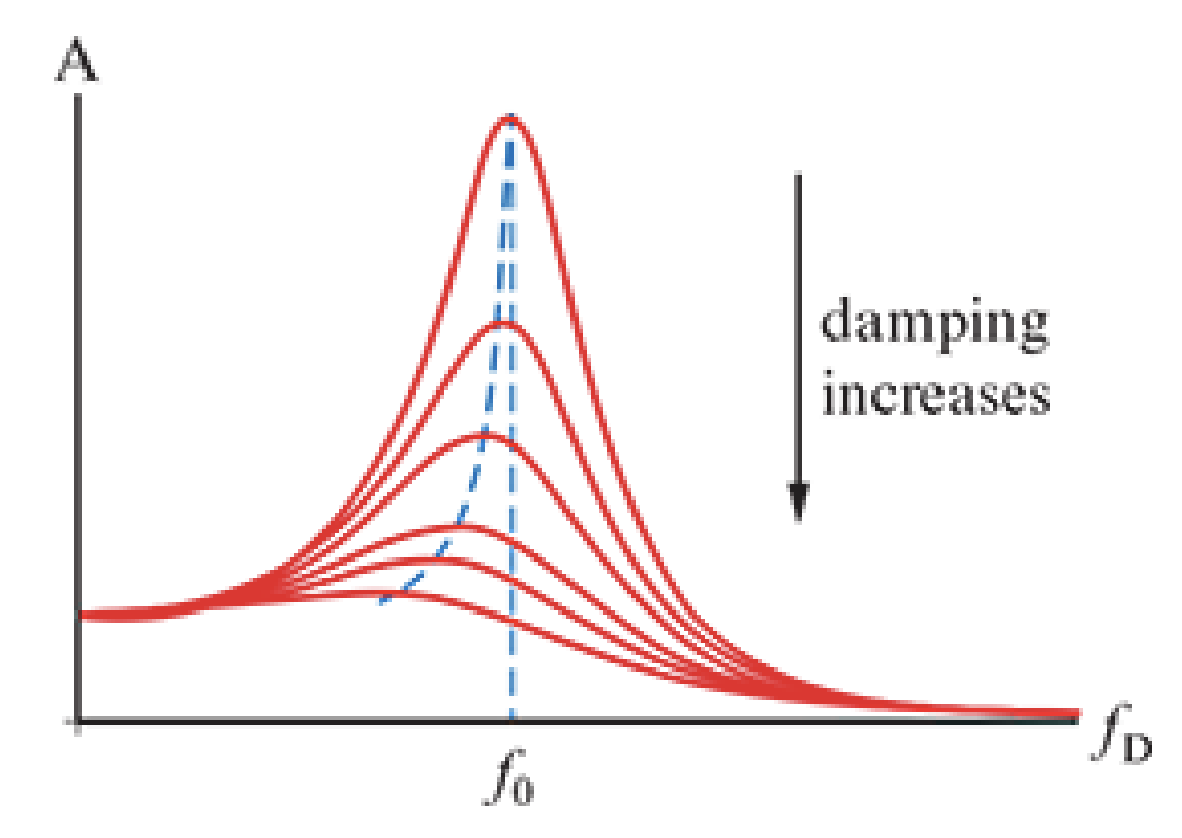
\includegraphics[width=0.4\linewidth]{Screenshot 2026-06-10 at 20.40.04.png}
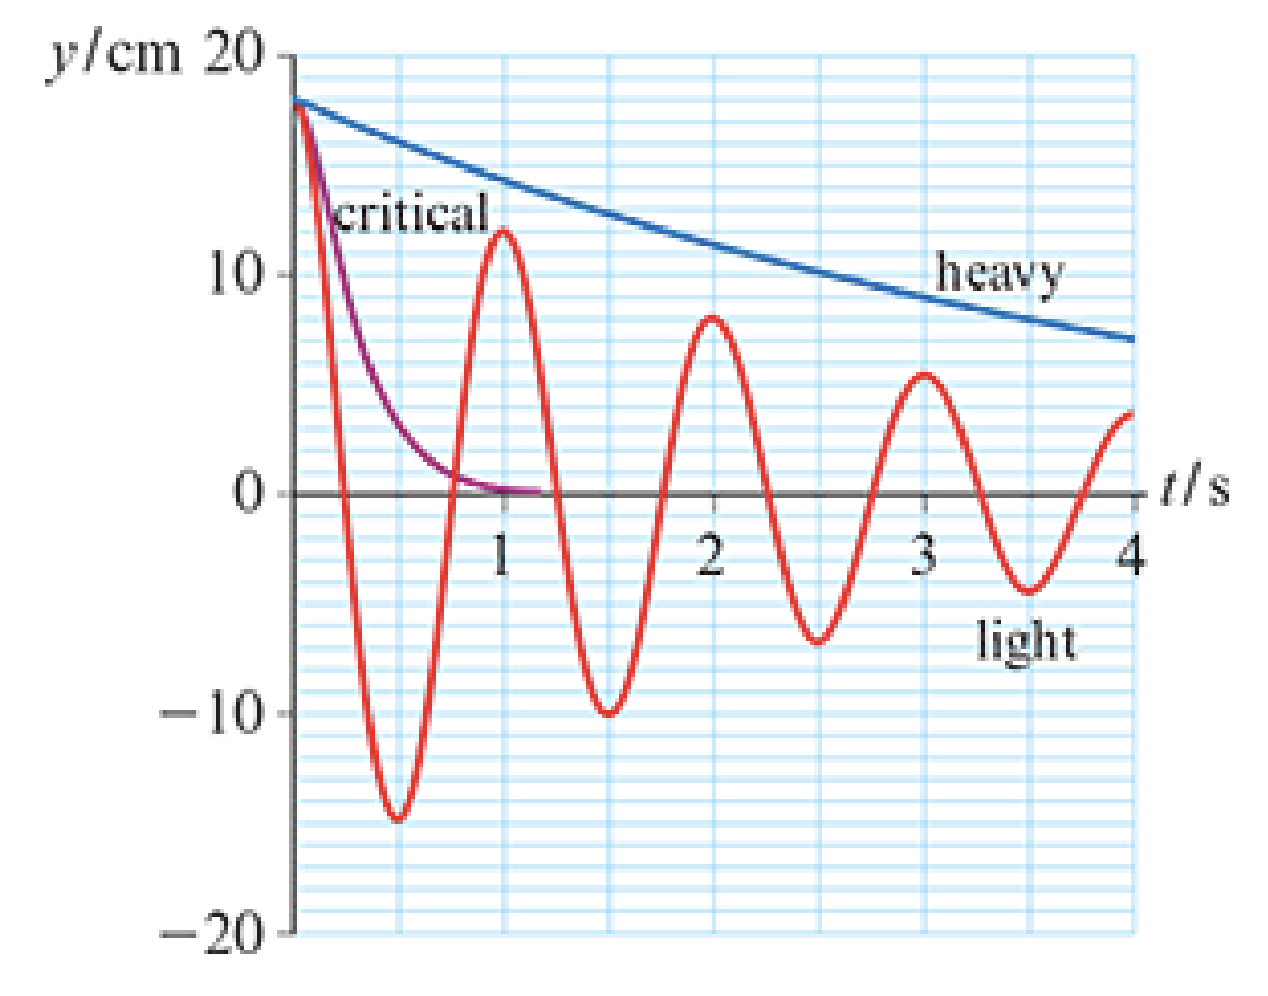
\includegraphics[width=0.4\linewidth]{Screenshot 2026-06-10 at 21.25.13.png}\\
The degree of damping increases as we move from the top curve down.\\
The blue dashed curve represents the peak of the curves (maximum amplitudes).
\end{center}
\begin{itemize}
  \item For very small damping, the peak of the curve occurs very close to the natural frequency of the system.\\
  When the driving frequency is equal to the natural frequency, the amplitude of oscillations is a maximum. This condition is called \textbf{Resonance}.
  \item As the amount of damping increases, the peak shifts to lower frequencies and becomes wider and shorter.
In other words, with large damping the amplitude is a maximum when the driving frequency is slightly less
than the natural frequency.
  \item At very low frequencies, the amplitude is essentially constant, and at high frequencies the amplitude goes
to zero.
\end{itemize}
Three cases regarding damping:
\begin{itemize}
  \item In light damping the system returns to
equilibrium after many oscillations of decreasing amplitude.
  \item In critical damping, the system returns to
equilibrium in the shortest possible time without performing oscillations.
  \item In the heavy or overdamped
case the system returns to equilibrium after a very long time without performing oscillations.
\end{itemize}
\newpage
\section{The Doppler effect}
It is more pronounced if the car going by is a Formula 1 racing car! (额V10那会儿可能效果最明显)\\
Me: I found a video with F1 cars that perfectly demonstrates Doppler effect! \\Lydia: You should wear a shirt that says "Doppler Effect" next Halloween...
\subsection{The Doppler effect at low speeds}
Definition: the change in the observed frequency of a wave when there is relative motion between the source and the observer.
\begin{center}
\begin{tikzpicture}[>=Stealth, scale=1.1]

    % --- Custom Color Definitions ---
    \colorlet{obsColor}{red!40!black!60}
    \colorlet{waveColor}{green!55!black!50}
    
    \def\observerSize{0.24}
    \def\observerLabelY{1.2}
    
    % --- Fixed Coordinates ---
    \coordinate (A) at (-5.0, 0);
    \coordinate (B) at (5.0, 0);
    \coordinate (source) at (1.5, 0); % Current location of the moving source

    % --- Stationary Observers (A and B) ---
    \foreach \observerPos/\labelVal in {A/A, B/B} {
        \fill[obsColor] (\observerPos) +(-\observerSize/2,-\observerSize/2) rectangle +(\observerSize/2,\observerSize/2);
        
        % Label letter below the square
        \node[anchor=north, inner sep=6pt] at (\observerPos) {\labelVal};
    }

    % --- Doppler Wavefronts (Perfect Right-Aligned Compression) ---
    % Every circle satisfies: (Center X) + (Radius) = 2.1
    % This forces them to perfectly align on the right side while expanding leftward.
    \draw[very thick, waveColor] (1.5, 0)   circle (0.6);   % Wave 1 (Newest)
    \draw[very thick, waveColor] (0.9, 0)   circle (1.2);   % Wave 2
    \draw[very thick, waveColor] (0.3, 0)   circle (1.8);   % Wave 3
    \draw[very thick, waveColor] (-0.3, 0)  circle (2.4);   % Wave 4
    \draw[very thick, waveColor] (-0.9, 0)  circle (3.0);   % Wave 5

    % Current location of the moving source (Blue dot)
    \fill[blue] (source) circle (0.13);

    % Velocity Vector Arrow (Red motion arrow passing through the waves)
    \draw[ultra thick, red, ->] (source) -- (3.6, 0);
    
    % "source moving" description placed neatly below the velocity arrow
    \node[anchor=north west, inner sep=2pt, color=black!90] 
        at (2.3, -0.1) {source moving};

\end{tikzpicture}
\end{center}
The large wavefront was emitted first. The position of the source when
this wavefront was emitted was at the center of this wavefront. The second wavefront was emitted later, and in
this time the position of the source moved to the right. So this wavefront has its center shifted to the right, and
similarly for the third wavefront.\\\\
Observer B will measure a higher frequency (number of wavefronts received per second) compared to observer A. For observer B, because of the bunching of the wavefronts, the wavelength measured will be less than the wavelength measured by the source. 
\subsubsection*{Doppler effect for light}
The approximate Doppler formula (when $v$ is small compared to $c$):
\[\dfrac{\Delta f}{f}=\dfrac{\Delta \lambda}{\lambda}\approx\dfrac{v}{c}\]
$\Delta f$ gives the change in observed frequency, or $\Delta\lambda$ gives the change in observed wavelength.\\\\
Redshift: Increase in $\lambda$, decrease in $f$.\\
Blueshift: Decrease in $\lambda$, increase in $f$.
\subsection{The Doppler effect for sound} 
\subsubsection*{Moving source and stationary observer}
\begin{center}
  \begin{tikzpicture}[>=Stealth, scale=1.2]

    % --- Define custom colors ---
    \colorlet{wavegreen}{green!60!black}
    \colorlet{sourceblue}{blue!70!cyan}
    \colorlet{usred}{red!80!black}

    % --- Top Part: t = 0 s ---
    \begin{scope}[yshift=4cm]
        % Source dot with green ring
        \draw[wavegreen, line width=1.5pt] (0,0) circle (0.15);
        \fill[sourceblue] (0,0) circle (0.12);

        % Green wavefront line (first)
        \draw[wavegreen, line width=1.2pt] (0, 1.2) -- (0, -1.5);
        
        % Label for first wavefront
        \node[anchor=south west, align=left, yshift=2pt] at (0, 1.2) {source emits first wavefront};

        % Label for source
        \node[anchor=east, xshift=-4pt] at (0,0) {source};

        % Arrow for source velocity u_s
        \draw[usred, ->, line width=1pt] (0.2, 0) -- (0.8, 0);
        
        % Label u_s with additional text
        \node[anchor=west, xshift=2pt] at (0.8,0) {$u_s$\quad towards stationary observer};

        % Time label t = 0 s
        \node[anchor=north, yshift=-4pt] at (0, -0.6) {$t=0$ s};
    \end{scope}

    % --- Reference dotted green lines connecting top and bottom ---
    \draw[wavegreen, line width=1.2pt, dashed, opacity=0.6] (0, 2.5) -- (0, 0.3);
    \draw[wavegreen, line width=1.2pt, dashed, opacity=0.6] (6.0, 1.3) -- (6.0, 0.3);

    % --- Bottom Part: t = 1 s ---
    \begin{scope}[yshift=1.2cm]
        % Distance arrow v (long arrow)
        \draw[<->, line width=0.8pt] (0, 1.1) -- (6.0, 1.1) node[midway, above] {$v$};

        % Source dot at second position (x = 1.4) with ring
        \draw[wavegreen, line width=1.5pt] (1.4,0) circle (0.15);
        \fill[sourceblue] (1.4,0) circle (0.12);
        
        % Arrow for source velocity u_s (second)
        \draw[usred, ->, line width=1pt] (1.6, 0) -- (2.0, 0);
        \node[anchor=west, xshift=2pt] at (2.0, 0) {$u_s$};

        % Green wavefront line (last) at source
        \draw[wavegreen, line width=1.2pt] (1.4, 1.0) -- (1.4, -1.0);
        % Green wavefront line (first) now here
        \draw[wavegreen, line width=1.2pt] (6.0, 1.0) -- (6.0, -1.0);

        % Top horizontal distance arrow split u_s and v-u_s
        \draw[<->, line width=0.8pt] (0, 0.2) -- (1.4, 0.2) node[midway, above] {$u_s$};
        \draw[<->, line width=0.8pt] (1.4, 0.2) -- (6.0, 0.2) node[midway, above] {$v - u_s$};

        % Lower dashed distance arrow
        \draw[<->, wavegreen, dashed, line width=1.2pt] (1.4, -0.2) -- (6.0, -0.2);

        % Label text blocks at the very bottom
        \begin{scope}[yshift=-1.2cm]
            \node[anchor=north, align=center, xshift=2pt] at (1.4, 0) {source emits last\\wavefront};
            \node[anchor=north, align=center] at (3.5, 1) {$f$ wavefronts in\\this distance};
            \node[anchor=north, align=center, xshift=-2pt] at (6.0, 0) {first wavefront\\now here};
        \end{scope}

        % Time label t = 1 s
        \node[anchor=north, yshift=-4pt] at (0, -0.4) {$t=1$ s};
    \end{scope}

\end{tikzpicture}
\end{center}
The stationary observer will measure a wavelength of $\lambda'=\dfrac{v-u_s}{f}=\dfrac{v}{f'}=\lambda\left(1\pm\dfrac{u_s}{v}\right)$ (where + is for source moving away, - for source approaching).\\
The frequency measured would then be $f'=\dfrac{v}{\lambda'}=f\left(\dfrac{v}{v\pm u_s}\right)$ (where + is for source moving away, - for source approaching).
\subsubsection*{Stationary source and moving observer}
\begin{center}
  \begin{tikzpicture}[>=Stealth, scale=1.2]

    % --- Define custom colors ---
    \colorlet{wavegreen}{green!60!black}
    \colorlet{obsblue}{blue!70!cyan}
    \colorlet{u0red}{red!80!black}

    % --- Top Part: t = 0 s ---
    \begin{scope}[yshift=4cm]
        % Observer dot with green ring at x = 6.0
        \draw[wavegreen, line width=1.5pt] (6.0,0) circle (0.15);
        \fill[obsblue] (6.0,0) circle (0.12);

        % Green wavefront lines (first encountered and the one to be encountered at t=1)
        \draw[wavegreen, line width=1.2pt] (6.0, 1.2) -- (6.0, -1.0);
        \draw[wavegreen, line width=1.2pt] (0.0, 1.2) -- (0.0, -1.0);
        
        % Label for first wavefront at observer
        \node[anchor=south, align=center, yshift=2pt] at (6.0, 1.2) {observer encounters\\first wavefront};
        
        % Label for wavefront at x=0
        \node[anchor=south, align=center, yshift=2pt] at (0.0, 1.2) {wavefront to be\\encountered at $t=1$ s};

        % Label for observer
        \node[anchor=west, xshift=4pt] at (6.0,0) {observer};

        % Arrow for observer velocity u_0 (pointing left towards source)
        \draw[u0red, ->, line width=1pt] (5.7, 0) -- (4.5, 0);
        
        % Label u_0 with additional text
        \node[anchor=south, yshift=2pt] at (4.8,0) {$u_0$ towards stationary source};

        % Time label t = 0 s
        \node[anchor=north, yshift=-4pt] at (0, -0.6) {$t=0$ s};
    \end{scope}

    % --- Reference dotted green lines connecting top and bottom ---
    \draw[wavegreen, line width=1.2pt, dashed, opacity=0.6] (0, 2.7) -- (0, 0.3);
    \draw[wavegreen, line width=1.2pt, dashed, opacity=0.6] (6.0, 2.7) -- (6.0, 0.3);

    % --- Bottom Part: t = 1 s ---
    \begin{scope}[yshift=1.2cm]
        % Top horizontal distance arrow showing the total relative distance v + u_0
        \draw[<->, line width=0.8pt] (0, 1.1) -- (6.0, 1.1) node[midway, above] {$v + u_0$};

        % Observer dot at second position (x = 4.5) with ring
        \draw[wavegreen, line width=1.5pt] (4.5,0) circle (0.15);
        \fill[obsblue] (4.5,0) circle (0.12);
        
        % Arrow for observer velocity u_0 (second)
        \draw[u0red, ->, line width=1pt] (4.2, 0) -- (3.6, 0);
        \node[anchor=south, yshift=2pt] at (3.9, 0) {$u_0$};

        % Green wavefront line (the one from x=0) now reaching the observer at x=4.5
        \draw[wavegreen, line width=1.2pt] (4.5, 0.2) -- (4.5, -1.0);
        
        % Horizontal distance arrows splitting the wave travel (v) and observer travel (u_0)
        \draw[<->, line width=0.8pt] (0, 0.2) -- (4.5, 0.2) node[midway, above] {$v$};
        \draw[<->, line width=0.8pt] (4.5, 0.2) -- (6.0, 0.2) node[midway, above] {$u_0$};

        % Lower dashed distance arrow framing the total measurement
        \draw[<->, wavegreen, dashed, line width=1.2pt] (0, -0.2) -- (6.0, -0.2);

        % Label text blocks at the very bottom
        \begin{scope}[yshift=-1.2cm]
            \node[anchor=north, align=center] at (4.5, 0) {observer encounters\\last wavefront};
            \node[anchor=north, align=center] at (2.5, 1) {measured wave speed\\is higher: $v + u_0$};
        \end{scope}

        % Time label t = 1 s
        \node[anchor=north, yshift=-4pt] at (0, -0.4) {$t=1$ s};
    \end{scope}

\end{tikzpicture}
\end{center}
It could be seen as, from the observer's perspective, that the source is moving. Note that here, the speed of sound relative to the observer is no longer $v$ as the medium has turned from still air to moving air.\\
Frequency observed would be given by $f'=f\dfrac{v+u_0}{v+u_0-u_0}=f\left(\dfrac{v\pm u_0}{v}\right)$ (where + is for observer approaching, - for observer moving away) The wavelength would be the same.
\newpage
% ===================== Unit D =====================
\unnumberedsection{Unit D Fields}
\section{Gravitation}
\subsection{Newton's law of gravitation}
A planet that orbits around the sun experiences acceleration, and thus a force is acting on it.\\
The attractive force of gravitation between two point masses (idealised bodies with no physical size) are:
\[F=G\dfrac{M_1M_2}{r^2}\]
where $G=6.67\times 10^{-11}\ \text{N\,m}^{2}\,\text{kg}^{-2}$, and $r$ is the center-to-center distance between the spherical bodies.\\
The direction of the force is along the line joining the two masses.\\
The gravitational force is always attractive. The magnitude of the force on each mass is the same.\\
(Spherical bodies with uniform distribution of mass can be considered as point mass, as the center of mass lies within the center of the spherical body.)
\subsubsection*{Gravitational Field Strength}
A mass $M$ is said to create a gravitational field in the space around it. 
A formal definition: region of space where a mass experiences a (gravitational) force.\\
The gravitational field strength, at a certain point, is the gravitational force per unit mass experienced by a small point mass m placed at that point: $g=\dfrac{F_\text{grav}}{m}$, or $\dfrac{GM}{r^2}$ for spherical bodies with mass $M$.\\
When height of an object is involved for calculating acceleration of the freefall, involve height in the radius of the formula as well.
\begin{center}
\begin{tikzpicture}[>=latex,scale=0.8]
    % Draw radial lines pointing inwards
    \foreach \angle in {0, 15, ..., 345} {
        \draw[
            cyan!70!blue, thick,
            postaction={decorate},
            % decoration={markings, mark=at position 0.65 with {\arrow{latex}}}
        ] (\angle:4) -- (\angle:0.4);
    }
    
    % Draw central mass/charge
    \filldraw[fill=orange!80!yellow, draw=orange!60!black, thick] (0,0) circle (0.4);
\end{tikzpicture}
\begin{tikzpicture}[>=latex]
    % Draw the uniform vertical lines
    \foreach \x in {0.5, 1.5, 2.5, 3.5, 4.5, 5.5, 6.5, 7.5, 8.5} {
        \draw[
            cyan!70!blue, thick,
            postaction={decorate},
            % decoration={markings, mark=at position 0.6 with {\arrow{latex}}}
        ] (\x, 5) -- (\x, 0);
    }
    
    % Draw the ground with a gradient and slanted right edge
    \shade[top color=brown!70!black, bottom color=white, draw=none] 
        (0,0) -- (9,0) -- (8.7,-0.8) -- (0,-0.8) -- cycle;
\end{tikzpicture}
\end{center}
The gravitational field strength around a single point or spherical mass is radial, which means that it points towards the centre of the mass creating the field. The field is not uniform: magnitude of $g$ decreases as we move away from $M$. \\
The other case: a uniform field with constant gravitational field strength. (e.g. constant $a$ of freefall)
\begin{center}
  \begin{tikzpicture}[>=latex]
        % Bottom axis
        \draw[->, thick] (-1, -1.5) -- (9, -1.5);
        
        % Dashed line connecting centers
        \draw[dashed, thick] (0.8,0) -- (7.6,0);
        
        % Mass M (Red)
        \filldraw[fill=red!70!white, draw=black] (0,0) circle (0.8);
        \node[above] at (0, 0.9) {$M$};
        \node[below] at (0, -0.8) {$x = 0$};
        
        % Mass m (Blue)
        \filldraw[fill=blue!70!white, draw=black] (8,0) circle (0.4);
        \node[above] at (8, 0.5) {$m$};
        \node[below] at (8, -0.8) {$x = d$};
    \end{tikzpicture}
  \end{center}
  At a point that is a distance x from the centre of the larger mass the net gravitational field strength is:
\[g=-\dfrac{GM}{x^2}+\dfrac{Gm}{(d-x)^2}\]
  \begin{center}
    \begin{tikzpicture}
        \begin{axis}[
            width=12cm, height=6.5cm,
            axis lines=middle,
            xmin=-0.1, xmax=1.05,
            ymin=-50, ymax=50,
            xtick={0, 0.2, 0.4, 0.6, 0.8, 1.0},
            ytick={-40, -20, 0, 20, 40},
            minor x tick num=3, % Creates 4 sub-intervals (0.05 steps)
            minor y tick num=3, % Creates 4 sub-intervals (5 unit steps)
            grid=both,
            grid style={line width=.1pt, draw=cyan!30},
            major grid style={line width=.2pt, draw=cyan!50},
            xlabel={$\dfrac{x}{d}$},
            ylabel={$g\,/\,\text{N\,kg}^{-1}$},
            every axis x label/.style={at={(ticklabel* cs:1.02)}, anchor=west},
            every axis y label/.style={at={(ticklabel* cs:1.02)}, anchor=south},
            % The formula plotted is proportional to the combined field of masses 16m and m
            domain=0.14:0.96,
            samples=200
        ]
            \addplot[red!80!black, thick] {0.1 * (-16/(x^2) + 1/((1-x)^2))};
        \end{axis}
    \end{tikzpicture}\\
    Variation of $g$ with distance from the larger mass.
\end{center}
Utilize this info for calculating the ratio of the masses: $\dfrac{M}{m}=\dfrac{x^2}{(d-x)^2}$; taking value of $x$ when $g=0$. 
\subsubsection*{Orbital Motion}
\begin{center}
  \begin{tikzpicture}
    % Define constants for scaling and sizing to control dimensions easily
    \def\orbitRadius{2.5cm} % Radius of the orbital path circle
    \def\planetRadius{0.8cm} % Radius of the central planet M
    \def\satelliteRadius{0.15cm} % Radius of the orbiting satellite m

    % Define key points for positioning elements
    \coordinate (origin) at (0,0); % Center point for planet M and orbit
    \coordinate (satPos) at (\orbitRadius, 0); % Current position of satellite m (right side)
    % End point for the radius vector line, chosen at 225 degrees (lower-left quadrant)
    \coordinate (r_end) at (225:{\orbitRadius});

    % --- Orbit ---
    % Black dashed circle to represent the orbital path
    \draw [dashed, thick, line width=1pt, color=black] (origin) circle (\orbitRadius);

    % --- Central Planet M ---
    % Define the planet with a radial shading from lighter blue inside to darker blue outside
    \node (planet) [
        circle,
        minimum size=2*\planetRadius, % Calculate diameter from radius constant
        inner sep=0pt,
        shading=radial,
        inner color=blue!20,
        outer color=blue!50,
        draw=black!30 % Subtle outline for clear definition
    ] at (origin) {};
    % Label 'M' placed above the planet node
    \node [above=0.25cm of planet, font=\large] {$M$};

    % --- Satellite m ---
    % Define the satellite as a small sphere with ball-style color shading for a 3D effect
    \node (satellite) [
        circle,
        minimum size=2*\satelliteRadius, % Calculate diameter from radius constant
        inner sep=0pt,
        ball color=lightgray,
        draw=gray % Subtle outline for definition
    ] at (satPos) {};
    % Label 'm' placed to the right of the satellite node
    \node [right=0.2cm of satellite, font=\large] {$m$};

    % --- Forces / Vectors ---
    % Define a global style for the vectors to ensure consistency in arrows
    % Uses a stealth arrowhead and thick line weights for visual clarity
    \tikzset{vectorStyle/.style={-stealth, ultra thick, line width=1.5pt}}

    % Red velocity vector - tangential to the orbit, pointing upwards from the satellite's position
    \draw [vectorStyle, red!90!black] (satPos) -- ++(0, 1.25cm);
    
    % Green gravitational force vector - radial, pointing directly from the satellite to the center (origin)
    \draw [vectorStyle, green!70!black] (satPos) -- (origin);

    % --- Radius Label r ---
    % Thin black double-headed arrow starting from origin to r_end at 225 degrees
    \draw [black, <->, thin] (origin) -- (r_end);
    
    % Positioning the math mode label 'r' next to the line segment.
    % The best appearance is achieved with manual placement next to the line's midpoint.
    % Line end is at approx (-1.77, -1.77) cm. Manual coordinate placement is chosen to match original diagram.
    \node [font=\large] at (-1.1cm, -0.9cm) {$r$}; 
    
\end{tikzpicture}
\end{center}
Gravitational force provides centripetal force. \\Judy: 碰到这种Planet的题先什么都不要想；先把这个写出来就有思路了。
\[\begin{aligned}
\dfrac{GMm}{r^2}&=\dfrac{mv^2}{r}\\
v&=\sqrt{\dfrac{GM}{r}}
\end{aligned}\] \[\begin{aligned}
\dfrac{GMm}{r^2}&=mr\dfrac{4\pi^2}{T^2}\\
T^2&=\dfrac{4\pi^2 r^3}{GM}
\end{aligned}\]
where $T$ is the time for one complete revolution, period of revolution.
\subsubsection*{Kepler's Laws}
\begin{itemize}
  \item First Law: planets move on ellipses with the sun at one of the foci of the ellipse. The length of the long axis of the ellipse (the major axis) is called 2a. This length is important for Kepler’s third law. (后面马上提到)
    \begin{center}
    \begin{tikzpicture}[scale=1.2]
    % ==========================================
    % Subfigure a
    % ==========================================
    \begin{scope}[shift={(0,0)}]
        % Subfigure label
        \node at (-2.3, 1.5) {\textbf{a}};
        
        % Main Ellipse
        \draw[thick, black!80] (0,0) ellipse (2.5 and 1.6);
        
        % Major Axis Dashed Line
        \draw[dashed, black!60, thick] (-2.5,0) -- (2.5,0);
        
        % Sun at Focus
        \filldraw[fill=yellow!90!orange, draw=black] (-1.1,0) circle (0.15);
        \node[below=4pt] at (-1.1,0) {Sun};
        
        % Planet
        \filldraw[fill=blue!40!cyan, draw=black] ({2.5*cos(40)},{1.6*sin(40)}) circle (0.09);
        
        % Vertex Labels
        \node[left=2pt] at (-2.5,0) {P};
        \node[right=2pt] at (2.5,0) {A};
    \end{scope}

    % ==========================================
    % Subfigure b
    % ==========================================
    \begin{scope}[shift={(6,0)}]
        % Subfigure label
        \node at (-2.3, 1.5) {\textbf{b}};
        
        % Main Ellipse
        \draw[thick, black!80] (0,0) ellipse (2.5 and 1.6);
        
        % Major Axis Length Representation (Blue double arrow)
        \draw[<->, >=Latex, cyan!80!blue, thick] (-2.5,0) -- (2.5,0);
        \node[below=4pt, fill=white, inner sep=2pt] at (0,0) {$2a$};
        
        % Random Point P on Ellipse
        \coordinate (P) at ({2.5*cos(55)},{1.6*sin(55)});
        \node[above right] at (P) {P};
        
        % Foci Positions
        \coordinate (F1) at (-1.1,0);
        \coordinate (F2) at (1.1,0);
        
        % Focal Lines to Point P
        \draw[thick, black!80] (F1) -- (P);
        \draw[thick, black!80] (F2) -- (P);
        
        % Foci Nodes
        \filldraw[fill=red!80!black, draw=black] (F1) circle (0.09);
        \node[below=4pt] at (F1) {$\text{F}_1$};
        
        \filldraw[fill=red!80!black, draw=black] (F2) circle (0.09);
        \node[below=4pt] at (F2) {$\text{F}_2$};
    \end{scope}
\end{tikzpicture}
  \end{center}

  \item Second Law: the line joining a planet and the sun sweeps equal areas in equal times.\\(Planet moves fastest at perihelion.)
\begin{center}
    \begin{tikzpicture}[scale=1.2]
    % ==========================================
    % Subfigure a
    % ==========================================
    \begin{scope}[shift={(0,0)}]
        % Subfigure label
        \node at (-2.3, 1.5) {\textbf{a}};
        
        % Ellipse geometry definitions
        % Center (0,0), a=2.5, b=1.6. Focus at (-1.1, 0)
        
        % Blue Sector (Near Sun / Perihelion side)
        \fill[blue!75!cyan!90!black] (-1.1,0) -- ({2.5*cos(130)},{1.6*sin(130)}) 
            arc(130:170:2.5 and 1.6) -- cycle;
            
        % Green Sector (Far from Sun / Aphelion side)
        \fill[green!60!black!80] (-1.1,0) -- ({2.5*cos(-10)},{1.6*sin(-10)}) 
            arc(-10:15:2.5 and 1.6) -- cycle;
            
        % Draw the main orbital path
        \draw[thick, black!80] (0,0) ellipse (2.5 and 1.6);
        
        % Sun
        \filldraw[fill=yellow!90!orange, draw=black] (-1.1,0) circle (0.15);
        \node[below=4pt] at (-1.1,0) {Sun};
        
        % Planet
        \filldraw[fill=blue!40!cyan, draw=black] ({2.5*cos(45)},{1.6*sin(45)}) circle (0.09);
        \node[left=3pt] at ({2.5*cos(45)},{1.6*sin(45)}) {Planet};
        
        % Motion Arrow
        \draw[->, >=Latex, thick, black!70] ({2.7*cos(22)},{1.75*sin(22)}) 
            arc(22:38:2.7 and 1.75);
            
        % Orbital Path Label
        \node[below] at (0, -0.9) {Orbital Path};
    \end{scope}
    \hfill
    % ==========================================
    % Subfigure b
    % ==========================================
    \begin{scope}[shift={(7,0)}]
        % Subfigure label
        \node at (-2.3, 1.5) {\textbf{b}};
        
        % Red Sector at Perihelion (Left side)
        \fill[red!80!black] (4.9-6,0) -- ({-2.5*cos(20)},{1.6*sin(20)}) 
            arc(160:200:2.5 and 1.6) -- cycle;
            
        % Red Sector at Aphelion (Right side)
        \fill[red!80!black] (4.9-6,0) -- ({2.5*cos(-5)},{1.6*sin(-5)}) 
            arc(-5:5:2.5 and 1.6) -- cycle;
            
        % Draw the orbital path
        \draw[thick, black!80] (0,0) ellipse (2.5 and 1.6);
        
        % Sun (S)
        \filldraw[fill=yellow!90!orange, draw=black] (4.9-6,0) circle (0.15);
        \node[below=4pt] at (4.9-6,0) {Sun};
        
        % Vertex Labels
        \node[left=2pt, font=\scriptsize] at (-2.5,0) {Perihelion};
        \node[right=2pt, font=\scriptsize] at (2.5,0) {Aphelion};
    \end{scope}
\end{tikzpicture}
\end{center}
  \item Third Law: the period of revolution of a planet around the sun is proportional to the $\dfrac{3}{2}$ power of the semi-major axis of the ellipse. $\left(T^2=\dfrac{4\pi^2 a^3}{GM}\right)$; $T^2\propto r^3$\\
  For a circular orbit with radius $r$, $r=a$. ($a$ shown as $2a$ when illustrating Kepler's First Law)
\end{itemize}
\subsection{Gravitational potential and energy}
The gravitational potential energy of two bodies is the work that was done in bringing the bodies to their present position from when they were infinitely far apart.
This energy is stored in the gravitational field.
\begin{center}
\begin{tikzpicture}[>=stealth, scale=0.95]
\definecolor{crimson}{rgb}{0.86, 0.08, 0.24}
\definecolor{forestgreen}{rgb}{0.13, 0.55, 0.13}
    % Define Styles
    \tikzstyle{massM} = [circle, draw=orange!60!black, fill=orange!70!brown, minimum size=2.4cm, line width=1.5pt]
    \tikzstyle{massm} = [circle, draw=orange!60!black, fill=orange!70!brown, minimum size=0.25cm, line width=1pt]

    % Coordinates
    \coordinate (M) at (0,0);
    \coordinate (m_near) at (4.5,0);
    \coordinate (m_mid) at (6.5,0);
    \coordinate (m_inf) at (9.5,0);

    % Draw Large Mass M
    \node[massM] at (M) {};
    \node[above=1.3cm] at (M) {$M$};

    % Draw Mass m at Infinity
    \node[massm] (inf_node) at (m_inf) {};
    \node[above=0.2cm] at (inf_node) {$m$ at infinity};

    % Draw Mass m brought near to M
    \node[massm] (near_node) at (m_near) {};
    \node[above=0.2cm] at (near_node) {$m$ brought near to $M$};

    % Draw connecting lines/arrows between the positions of m
    \draw[line width=1pt] (m_near) -- (m_mid);
    \draw[dashed, line width=1pt] (m_mid) -- (m_inf);

    % Red and Green Arrows on the near mass
    \draw[->, crimson, line width=1.5pt] (m_near) -- ++(-1.1,0);
    \draw[->, forestgreen, line width=1.5pt] (m_near) -- ++(1.1,0);

    % Text label below the line
    \node[below=0.2cm] at (5.8,-0.1) {force does work};

    % Distance indicator r below the setup
    \def\yoffset{-1.4}
    \draw[<->, line width=0.8pt] (0,\yoffset) -- (4.5,\yoffset) node[midway, fill=white, inner sep=3pt] {$r$};

\end{tikzpicture}\\
$^*:$ Assume $M$ is fixed and that only $m$ has moved.\\
This energy belongs to the pair of masses $M$ and $m$ and not just to one of them. \\
(Assume no kinetic energy is involved. Masses move at a small constant speed.)
\end{center}
The total work done in moving the mass $m$ from infinity to a distance $r$ from the centre of a spherical mass $M$ is:
\[W=\int_{\infty}^{r}\dfrac{GMm}{r^2}\mathrm{d}r=-\left[\dfrac{GMm}{r}\right]^r_{\infty}=-\dfrac{GMm}{r}\Rightarrow E_p=-\dfrac{GMm}{r}\]
Why is the gravitational potential energy negative:
\begin{itemize}
  \item Note that the force is directed to the right, while the motion is directed left.
  \item No potential energy initially $\Rightarrow$ Increase $E_K$ for $m$ and decreased potential energy overall
\end{itemize}
\begin{center}
  \begin{tikzpicture}[>=stealth, scale=1.2]

    % Define colors
    \definecolor{planetTop}{RGB}{41, 128, 185}
    \definecolor{planetBottom}{RGB}{39, 174, 96}

    % 1. Draw the planet surface (shaded curvature at the bottom)
    \begin{scope}
        \clip (-3.5,-0.5) rectangle (3.5,1.5);
        \shade[top color=planetTop, bottom color=planetBottom] (0,-4) circle (4.5);
    \end{scope}


    % 2. Draw the potential well (dashed lines)
    % Left upper plateau
    \draw[thick, dashed, black!70] (-3.5, 4.5) -- (-1.2, 4.5);
    % Right upper plateau
    \draw[thick, dashed, black!70] (1.2, 4.5) -- (3.5, 4.5);
    % Left slope down to the surface
    \draw[thick, dashed, black!70] (-1.2, 4.5) -- (-0.3, 0.55);
    % Right slope down to the surface
    \draw[thick, dashed, black!70] (1.2, 4.5) -- (0.3, 0.55);
    % Bottom flat part of the well
    \draw[thick, dashed, black!70] (-0.3, 0.55) -- (0.3, 0.55);

    % 3. Draw the object (orange sphere resting on the surface)
    \draw[fill=orange!90!brown] (0, 0.7) circle (0.15);
    \draw[darkgray, thin] (0, 0.7) circle (0.15);

    % 4. Text Labels and Equations
    % Top label: "very far away E_P = 0" (Changed 'anchor=bottom' to 'above')
    \node[above, align=center] at (0, 4.5) {very far away $E_{\text{P}} = 0$};

    % Left label: "potential well"
    \node[anchor=east] at (-1.4, 3.0) {potential well};

    % Right label: Equation for potential energy at the surface
    \node[anchor=west] at (0.6, 0.7) {$E_{\text{P}} = -\dfrac{GMm}{R}$};

\end{tikzpicture}
\end{center}
\subsubsection*{Gravitational Potential}
The gravitational potential, $V_g$, at a point $P$ in a gravitational field is the work done per unit mass in bringing a small point mass from infinity to point $P$. 
\[V_g=\dfrac{W}{m}=-\dfrac{GM}{r};\ E_p=mV_g;\ W=m\Delta V_g\]
where $W$ is the work done on the mass by the external agent moving the mass.
\subsubsection*{Field and potential}
Gravitional field strength can be calculated using:
\[g=\dfrac{\Delta V_g}{\Delta r}\left(=-\dfrac{dV_g}{dr}\right)\]
where $\Delta r$ is the difference between two points close to each other and $\Delta V_g$ is the difference between gravitational potential.
\subsubsection*{Equipotential surface}
An equipotential surface consists of points (that have same distance from the source) that have the same gravitational potential.
\begin{center}
\begin{tikzpicture}[>=stealth, font=\small, scale=2]

% Colors
\definecolor{mygreen}{rgb}{0.5, 0.8, 0.5}
\definecolor{myfieldred}{rgb}{0.9, 0.2, 0.2}
\definecolor{mygrey}{rgb}{0.5, 0.5, 0.5}

% Radial Potential Shading
\foreach \r in {0.0, 0.05, ..., 1.1}
{
    \pgfmathsetmacro{\opacity}{0.8 * (1.1 - \r)/1.1 + 0.15}
    \draw[mygreen, fill=mygreen, fill opacity=\opacity, draw opacity=0] (0,0) circle (\r + 0.05);
}

% Background circle (lightest green) for potential shading base
%\fill[mygreen!20] (0,0) circle (1.1);

% Draw the planet core shadow/gradient
\begin{scope}
    \clip (0,0) circle (0.3);
    \fill[mygreen!40] (0,0) circle (0.3);
    \shade[inner color=mygreen!80, outer color=mygreen!40] (0,0) circle (0.3);
\end{scope}
\draw[mygrey] (0,0) circle (0.3);

% Potential Lines (Concentrated near core)
\draw[mygrey] (0,0) circle (0.43);
\draw[mygrey] (0,0) circle (0.61);
\draw[mygrey] (0,0) circle (0.91);

% "field lines" text with thin line pointing to a field line
\node[anchor=south west, text width=2cm, align=left] (fl-text) at (-1.3, 1.3) {field lines};

% Field Lines with Arrows (Red, pointing inwards)
% Angle logic and careful placement to match the image
\pgfmathsetmacro{\fieldlinecount}{12}
\foreach \i in {1,...,\fieldlinecount}
{
    \pgfmathsetmacro{\angle}{(\i-1)*360/\fieldlinecount}
    % Outer red lines, pointing towards core
    \draw[->, thick, myfieldred] (\angle:1.4) -- (\angle:1.0);
    % Inner red lines (continuing the path)
    \draw[myfieldred] (\angle:1.0) -- (\angle:0.3);
}

% Add boundary line of the potential shading, for crisp finish
\draw[mygrey] (0,0) circle (1.1);

\end{tikzpicture}
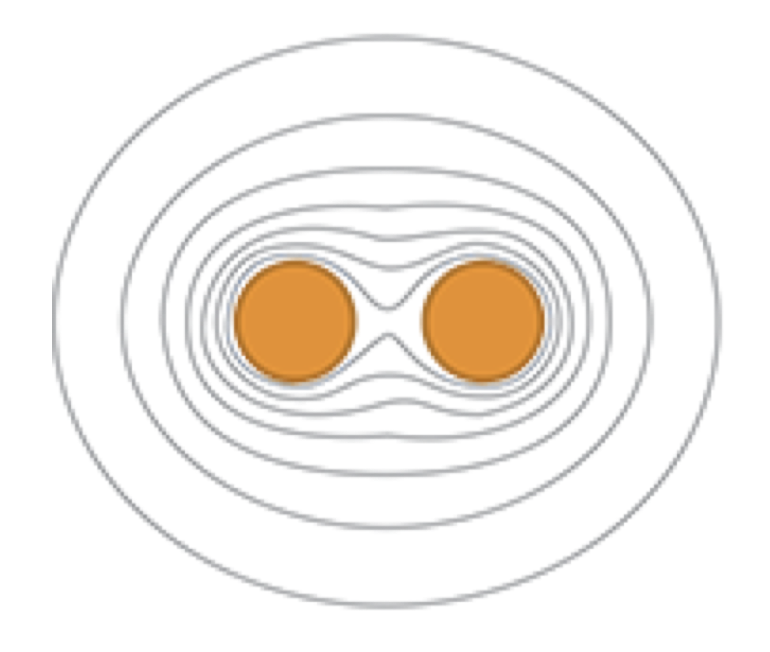
\includegraphics[width=0.3\linewidth]{Screenshot 2026-06-16 at 01.33.33.png}
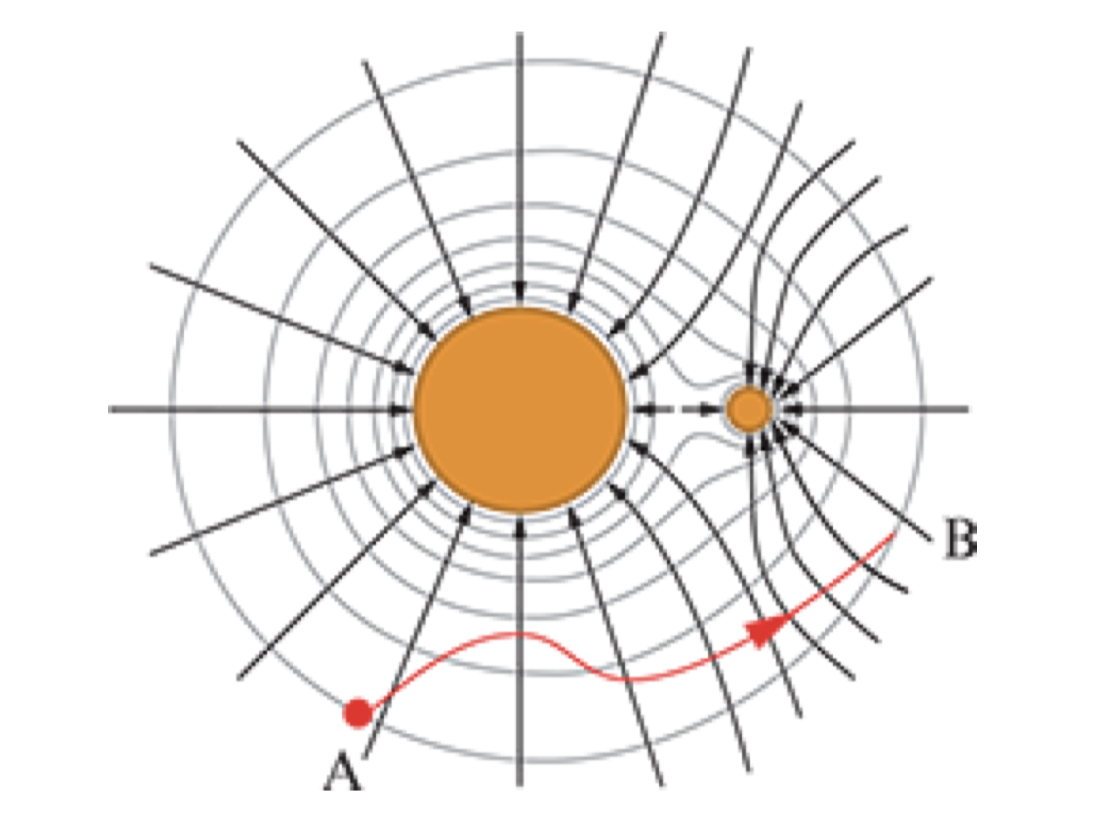
\includegraphics[width=0.33\linewidth]{Screenshot 2026-06-16 at 01.33.54.png}\\
\end{center}
Equipotential surfaces for two equal spherical masses and two unequal masses. Field lines are normal to the equipotential surfaces.
The work done to move a point mass from one point to another point on the same equipotential surface (from A to B) is zero: $\Delta V_g=0$.
\subsection{Motion in a gravitational field}
\begin{center}
\begin{tikzpicture}[scale=1.05, >=latex]

% Draw shaded central mass M sphere
\filldraw[inner color=blue!10, outer color=blue!30, draw=blue!60!black] (0,0) circle (0.6cm);
\node at (0,0) {\Large $M$};

% Draw dashed circular orbit line
\draw[dashed, gray!80, thick] (0,0) circle (3cm);

% Draw grey double-headed radius arrow
\draw[<->, gray, thin] (0,0) -- (40:3cm) node[midway, sloped, above] {$r$};

% Define coordinate for satellite m
\coordinate (pos_m) at (150:3cm);

% Draw centripetal force vector F arrow, green, toward origin
% Using ++ updates the internal coordinate, allowing 'midway' to place the label automatically
\draw[->, green!70!black, thick] (pos_m) -- ++(-30:1.3cm) node[midway, below left] {$F$};

% Draw tangential velocity vector v arrow, red, tangential
\draw[->, red, thick] (pos_m) -- ++(60:1.3cm) node[above left, yshift=-2pt] {$v$};

% Draw shaded satellite m body sphere (drawn last so arrows sit cleanly underneath)
\filldraw[inner color=purple!40, outer color=purple, draw=purple!80!black] (pos_m) circle (0.15cm);

% Label for mass m body
\node[above left] at (pos_m) {$m$};

\end{tikzpicture}
\begin{tikzpicture}[scale=0.9]
\begin{axis}[
    width=12cm, height=9cm,
    xmin=1, xmax=8.2,
    ymin=-65, ymax=35,
    axis lines=middle,
    clip=false, % Ensures labels outside the axis box aren't cut off
    % Grid settings mimicking graph paper
    grid=both,
    minor tick num=3,
    minor tick style={line width=.1pt, draw=blue!20},
    major tick style={line width=.2pt, draw=blue!50},
    % Customizing ticks to match the layout
    ytick={-60, -40, -20, 0, 20},
    major tick length=0pt,
    yticklabels={ , , , , }, % Handled safely via the invoke loop below
    xtick={2, 4, 6, 8},
    extra x ticks={1}, 
    extra x tick labels={ }, 
    xlabel={r/R},
    xlabel style={at={(axis cs: 8.2, 0)}, anchor=north east, yshift=-10pt, font=\small},
    ylabel={},
    samples=150
    ]

% Plots with ultra thick lines
\addplot[red, ultra thick, domain=1:8] {30/x};
\addplot[blue, ultra thick, domain=1:8] {-30/x};
\addplot[orange, ultra thick, domain=1:8] {-60/x};

% Safe loop invocation using #1 instead of \y to avoid deferred expansion errors
\pgfplotsinvokeforeach{-60,-40,-20,0,20}{
    \node[anchor=east, xshift=-12pt, font=\small, text=black] at (axis cs: 1, #1) {#1};
}

% Labels next to curves near their starting points
\node[anchor=east, xshift=-2pt, text=red, font=\small] at (axis cs: 1, 30) {$E_K$};
\node[anchor=east, xshift=-2pt, text=blue, font=\small] at (axis cs: 1, -30) {$E_T$};
\node[anchor=east, xshift=-2pt, text=orange, font=\small] at (axis cs: 1, -60) {$E_P$};

% Rotated vertical Y-axis label using relative coordinates (safe from xmin/xmax boundaries)
\node[rotate=90, text=blue!70!black, font=\small] at (rel axis cs: -0.12, 0.5) {Energy / MJ};

\end{axis}
\end{tikzpicture}
\end{center}
\[E_T=E_K+E_p=\dfrac{1}{2}mv^2-\dfrac{GMm}{r}=\dfrac{1}{2}m\left(\sqrt{\dfrac{GM}{r}}\right)^2-\dfrac{GMm}{r}=-\dfrac{GMm}{2r}\]
\begin{itemize}
  \item If the total energy is positive, the object will follow a hyperbolic path and never return.
  \item If the total energy is zero, the object will follow a parabolic path to infinity, where it will just about stop. It will never return.
  \item If the total energy is negative, the object will go into a circular or elliptical orbit (or crash into the planet if the launching speed is too low).
\end{itemize}
\begin{center}
  \begin{tikzpicture}[>=Stealth, font=\small]

% Central object (blue shaded sphere) at origin (focus)
\node[circle, ball color=blue!60!white, minimum size=0.7cm, inner sep=0pt] (sphere) at (0,0) {};
% Highlight on the central object
\node[circle, fill=white!70!blue!30, minimum size=0.15cm, inner sep=0pt] at ($(sphere.north west)!0.3!(sphere.center)$) {};

% Starting point for all paths (launch point)
\coordinate (Start) at (0, 0.5);

% Straight Line Path
\draw[red, thick, -{Stealth}] (Start) -- (0, 1) node[above, text=black] {straight line};

% Closed Path: Circle or Ellipse
% Closed bezier path that passes through (Start) and surrounds the origin
\draw[red, thick] (Start) .. controls (-0.8, 0.5) and (-0.8, -1.5) .. (0, -1.5)
                          .. controls (0.8, -1.5) and (0.8, 0.5) .. (Start) -- cycle;
% Label for the elliptical path, centered below it
\node[anchor=north, align=center, text width=3.5cm] at (0, -1.6) {circle or ellipse \\ $E_{\text{K}} + E_{\text{P}} < 0$};

% Open Path 1: Hyperbola
% Gentler curve fanning out to the top right
\draw[red, thick, -{Stealth}] (Start) .. controls (2.0, 0.2) and (3.0, -0.3) .. (4.0, -0.5);
% Label for the hyperbola, positioned below the arrow end
\node[anchor=south west, align=left, text width=3cm, yshift=0.3cm] at (4.0, -0.8) {hyperbola 双曲线\\ $E_{\text{K}} + E_{\text{P}} > 0$};

% Open Path 2: Parabola
% More curved path fanning to the bottom right, between the hyperbola and ellipse
\draw[red, thick, -{Stealth}] (Start) .. controls (1.8, 0.1) and (2.6, -0.8) .. (3.2, -1.4);
% Label for the parabola, positioned below the arrow end
\node[anchor=south west, align=left, text width=3cm, yshift=0.3cm] at (3.2, -2.4) {parabola 抛物线\\ $E_{\text{K}} + E_{\text{P}} = 0$};
\end{tikzpicture}
\end{center}
\subsubsection*{Escape speed}
Escape speed is the minimum speed a body in a gravitational field must have in order to reach infinity.\\
The condition to escape from any point in a gravitational field is that the total energy at that point must be zero.
\[v_\text{esc}=\sqrt{\dfrac{2GM}{r}}\]
\subsubsection*{Reasons behind weightlessness}
Essentially, the resultant force on the astronaut is zero. \\
In the case where $W$ is the weight, $F$ is the net force, $N$ is the reaction force from the floor of the spacecraft:
\[
\begin{aligned}
  F&=W-N\\
  &\Downarrow\\
  N&=W-F\\
  &=\dfrac{GMm}{r^2}-\dfrac{mv^2}{r}\\
  &=\dfrac{m}{r}\left(\dfrac{GM}{r}-v^2\right)\\
  \because v^2_\text{orbit}&=\dfrac{GM}{r}\\
  \therefore N&=0
\end{aligned}
\]
\section{Electric and magnetic fields}
\subsection{Electric charge, force and field}
Properties of electric charges:
\begin{enumerate}
  \item Law of conservation applies to electric charges: they can't be created or destroyed.
  \item It is a quantizied quantity: this means that the amount of electric charge on a body is always an integral multiple of a basic unit. ($1e=1.6\times 10^{-19}$ C)
\end{enumerate}
\begin{center}
  % Define common styles for consistency across the grid
\tikzset{
    benchline/.style={black, thin},
    stand/.style={draw=black, fill=gray!30, thin},
    sphere/.style={draw=black, fill=cyan!15, thin},
    rod/.style={draw=black, fill=white, thin},
    wire/.style={black, thin},
    flowarrow/.style={-Latex, blue, thin},
    chargeLabel/.style={font=\tiny, inner sep=0.5pt}
}

% Custom ground symbol pic definition
\tikzset{
    pics/ground/.style={
        code={
            \draw[black, thin] (0,0) -- (0,-0.2);
            \draw[black, thin] (-0.3,-0.2) -- (0.3,-0.2);
            \draw[black, thin] (-0.2,-0.28) -- (0.2,-0.28);
            \draw[black, thin] (-0.1,-0.36) -- (0.1,-0.36);
        }
    }
}

\begin{tikzpicture}

% Grid layout parameters for easy positioning of elements
\def\dx{3.8} % Horizontal separation between columns
\def\dy{-3.2} % Vertical separation between rows

% ========================================================================
% TOP ROW: Inducing charge with a Positive and a Negative Rod
% ========================================================================

% Diagram (1,1) [Top-Left]: Neutral sphere near a positive rod
\begin{scope}[shift={(0,0)}]
    \draw[benchline] (-1.2,0) -- (1.2,0);
    \draw[stand] (-0.1,0) rectangle (0.1,1.0);
    \draw[sphere] (0, 1.5) circle (0.5);
    \draw[rod] (0.8, 1.3) rectangle (1.6, 1.7);
    % Sphere Induced Charges: Negative attracted, positive repelled
    \node[chargeLabel] at (-0.28, 1.78) {+}; \node[chargeLabel] at (-0.28, 1.22) {+};
    \node[chargeLabel] at ( 0.28, 1.78) {-}; \node[chargeLabel] at ( 0.28, 1.22) {-};
    % Rod Charges: Positive
    \node[chargeLabel] at (1.0, 1.5) {+}; \node[chargeLabel] at (1.4, 1.5) {+};
\end{scope}

% Diagram (1,2) [Top-Right]: Neutral sphere near a negative rod
\begin{scope}[shift={(\dx,0)}]
    \draw[benchline] (-1.2,0) -- (1.2,0);
    \draw[stand] (-0.1,0) rectangle (0.1,1.0);
    \draw[sphere] (0, 1.5) circle (0.5);
    \draw[rod] (0.8, 1.3) rectangle (1.6, 1.7);
    % Sphere Induced Charges: Positive attracted, negative repelled
    \node[chargeLabel] at (-0.28, 1.78) {-}; \node[chargeLabel] at (-0.28, 1.22) {-};
    \node[chargeLabel] at ( 0.28, 1.78) {+}; \node[chargeLabel] at ( 0.28, 1.22) {+};
    % Rod Charges: Negative
    \node[chargeLabel] at (1.0, 1.5) {-}; \node[chargeLabel] at (1.4, 1.5) {-};
\end{scope}

% ========================================================================
% MIDDLE ROW: Grounding to remove repelled induced charges
% ========================================================================

% Diagram (2,1) [Middle-Left]: Grounding the far side near a positive rod
\begin{scope}[shift={(0,\dy)}]
    \draw[benchline] (-1.2,0) -- (1.2,0);
    \draw[stand] (-0.1,0) rectangle (0.1,1.0);
    \draw[sphere] (0, 1.5) circle (0.5);
    \draw[rod] (0.8, 1.3) rectangle (1.6, 1.7);
    % Grounding Wire & Symbol
    \draw[wire] (-0.35, 1.6) -| (-0.7, 0); \pic at (-0.7, 0) {ground};
    % Electron flow arrow pointing UP: Earth acts as electron source to neutralise positive far side
    \draw[flowarrow] (-0.9, 0.0) -- (-0.9, 1.5);
    \node[font=\footnotesize, anchor=east] at (-0.95, 0.75) {electrons};
    % Induced Charges: same distribution as (1,1)
    \node[chargeLabel] at (-0.28, 1.78) {+}; \node[chargeLabel] at (-0.28, 1.22) {+};
    \node[chargeLabel] at ( 0.28, 1.78) {-}; \node[chargeLabel] at ( 0.28, 1.22) {-};
    \node[chargeLabel] at (1.0, 1.5) {+}; \node[chargeLabel] at (1.4, 1.5) {+};
\end{scope}

% Diagram (2,2) [Middle-Right]: Grounding the far side near a negative rod
\begin{scope}[shift={(\dx,\dy)}]
    \draw[benchline] (-1.2,0) -- (1.2,0);
    \draw[stand] (-0.1,0) rectangle (0.1,1.0);
    \draw[sphere] (0, 1.5) circle (0.5);
    \draw[rod] (0.8, 1.3) rectangle (1.6, 1.7);
    % Grounding Wire & Symbol
    \draw[wire] (-0.35, 1.6) -| (-0.7, 0); \pic at (-0.7, 0) {ground};
    % Electron flow arrow pointing DOWN: Electrons are repelled from negative far side to ground
    \draw[flowarrow] (-0.9, 1.5) -- (-0.9, 0.0);
    \node[font=\footnotesize, anchor=east] at (-0.95, 0.75) {electrons};
    % Induced Charges: same distribution as (1,2)
    \node[chargeLabel] at (-0.28, 1.78) {-}; \node[chargeLabel] at (-0.28, 1.22) {-};
    \node[chargeLabel] at ( 0.28, 1.78) {+}; \node[chargeLabel] at ( 0.28, 1.22) {+};
    \node[chargeLabel] at (1.0, 1.5) {-}; \node[chargeLabel] at (1.4, 1.5) {-};
\end{scope}

% ========================================================================
% BOTTOM ROW: Charged Spheres after process is complete
% ========================================================================

% Diagram (3,1) [Bottom-Left]: Remaining charge after ground and positive rod removal. Net Negative.
\begin{scope}[shift={(0,2*\dy)}]
    \draw[benchline] (-1.2,0) -- (1.2,0);
    \draw[stand] (-0.1,0) rectangle (0.1,1.0);
    \draw[sphere] (0, 1.5) circle (0.5);
    % Sphere now has net negative charge after grounding away repelled positive.
    \node[chargeLabel] at (-0.15, 1.5) {-}; \node[chargeLabel] at (0.15, 1.5) {-};
\end{scope}

% Diagram (3,2) [Bottom-Right]: Remaining charge after ground and negative rod removal. Net Positive.
\begin{scope}[shift={(\dx,2*\dy)}]
    \draw[benchline] (-1.2,0) -- (1.2,0);
    \draw[stand] (-0.1,0) rectangle (0.1,1.0);
    \draw[sphere] (0, 1.5) circle (0.5);
    % Sphere now has net positive charge after grounding away repelled negative.
    \node[chargeLabel] at (-0.15, 1.5) {+}; \node[chargeLabel] at (0.15, 1.5) {+};
\end{scope}

\end{tikzpicture}
\begin{tikzpicture}[>=stealth]

    % Row 1
    \begin{scope}[shift={(0,0)}]
        % Positive charge q1
        \draw[red!70, fill=red!15, thick, opacity=0.8] (0,0) circle (0.5);
        \node[red!90, font=\bfseries] at (0,0) {$+$};
        \node[font=\small] at (0,0.7) {$q_1$};
        % Negative charge q2
        \draw[blue!70, fill=blue!15, thick, opacity=0.8] (4,0) circle (0.5);
        \node[blue!90, font=\bfseries] at (4,0) {$-$};
        \node[font=\small] at (4,0.7) {$q_2$};
        % Force arrows (attraction)
        \draw[->, green!60!black, thick] (0.2,0) -- (1.5,0);
        \draw[->, green!60!black, thick] (3.8,0) -- (2.5,0);
    \end{scope}

    % Row 2
    \begin{scope}[shift={(0,-2.5)}]
        % Two positive charges (repulsion)
        \draw[red!70, fill=red!15, thick, opacity=0.8] (0,0) circle (0.5);
        \node[red!90, font=\bfseries] at (0,0) {$+$};
        \draw[red!70, fill=red!15, thick, opacity=0.8] (4,0) circle (0.5);
        \node[red!90, font=\bfseries] at (4,0) {$+$};
        % Force arrows (repulsion)
        \draw[->, green!60!black, thick] (-0.2,0) -- (-1.5,0);
        \draw[->, green!60!black, thick] (4.2,0) -- (5.5,0);
    \end{scope}

    % Row 3
    \begin{scope}[shift={(0,-5.0)}]
        % Two negative charges (repulsion)
        \draw[blue!70, fill=blue!15, thick, opacity=0.8] (0,0) circle (0.5);
        \node[blue!90, font=\bfseries] at (0,0) {$-$};
        \draw[blue!70, fill=blue!15, thick, opacity=0.8] (4,0) circle (0.5);
        \node[blue!90, font=\bfseries] at (4,0) {$-$};
        % Force arrows (repulsion)
        \draw[->, green!60!black, thick] (-0.2,0) -- (-1.5,0);
        \draw[->, green!60!black, thick] (4.2,0) -- (5.5,0);
    \end{scope}

    % Distance label r
    \draw[<->, draw=gray, thin] (0,-6.3) -- (4,-6.3) node[midway, above, text=black] {$r$};

\end{tikzpicture}
\end{center}
Coulomb's Law states that, the electric force between two point charges $q_1$ and $q_2$ that is separated by a distance of $r$ is given by
\[F=k\dfrac{q_1q_2}{r^2}\]
where $k=\dfrac{1}{4\pi\varepsilon}$ is the Coulomb constant (the $\varepsilon$ is the permittivity).\\
($k=8.99\times 10^{9}\ \text{N\,m}^{2}\,\text{C}^{-2}$, $\varepsilon=8.85\times 10^{-12}\ \text{C}^{2}\,\text{N}^{-1}\,\text{m}^{-2}$ (in vacuum))
\subsubsection*{Electric Field}
Electric Field Strength, $E$, is the electric force per unit charge experienced by a small, positive, point charge $q$: $\vec{E}=\dfrac{\vec{F}}{q}$.
The direction of the electric field is the same as the direction of the force experienced by a positive charge at the given point.\\
The formula $E=k\dfrac{Q}{r^2}$ applies to a point charge / outside of the spherical charge.
\begin{center}
  \tikzset{
    % Standard field line style with an arrow centered along the path
    fieldline/.style={
        draw=red!70!black,
        thick,
        postaction={decorate, decoration={markings, mark=at position 0.55 with {\arrow{Stealth[scale=1.1]}}}}
    },
    % Node style for the point charges
    charge/.style={
        circle,
        draw=black,
        fill=white,
        inner sep=1.5pt
    }
}

\begin{tikzpicture}[scale=0.6]

    % ========================================================================
    % LEFT DIAGRAM: Like Charges (Repulsion Configuration)
    % ========================================================================
    \begin{scope}[shift={(0,0)}]
        % Outer boundary frame
        \draw[thin, gray] (-4,-3.2) rectangle (4,3.2);
        
        % Generate 4-way quadrant symmetry automatically
        \foreach \xsym in {1, -1} {
            \foreach \ysym in {1, -1} {
                \begin{scope}[xscale=\xsym, yscale=\ysym]
                    % Radial lines facing outward
                    \draw[fieldline] (1.6,0) -- (3.9,0);
                    \draw[fieldline] (1.6,0) .. controls (2.4,0.3) and (3.4,0.7) .. (3.9,1.1);
                    \draw[fieldline] (1.6,0) .. controls (2.3,0.7) and (3.2,1.6) .. (3.5,2.9);
                    
                    % Lines bending vertically near the center line
                    \draw[fieldline] (1.6,0) .. controls (1.7,1.1) and (2.1,2.3) .. (2.4,2.9);
                    \draw[fieldline] (1.6,0) .. controls (1.3,1.0) and (1.1,2.1) .. (1.3,2.9);
                    \draw[fieldline] (1.6,0) .. controls (0.9,0.5) and (0.4,1.4) .. (0.4,2.9);
                    
                    % Central axis lines approaching the neutral point
                    \draw[fieldline] (1.6,0) -- (0.2,0);
                    \draw[fieldline] (0,0.2) -- (0,2.9);
                \end{scope}
            }
        }
        
        % Charge markers and labels
        \node[charge] (q1_left) at (-1.6,0) {};
        \node[below=4pt, font=\small] at (q1_left) {$q_1$};
        
        \node[charge] (q2_left) at (1.6,0) {};
        \node[below=4pt, font=\small] at (q2_left) {$q_2$};
    \end{scope}

    % ========================================================================
    % RIGHT DIAGRAM: Opposite Charges (Dipole Configuration)
    % ========================================================================
    \begin{scope}[shift={(9,0)}]
        % Outer boundary frame
        \draw[thin, gray] (-4,-3.2) rectangle (4,3.2);
        
        % Generate top/bottom symmetry automatically
        \foreach \ysym in {1, -1} {
            \begin{scope}[yscale=\ysym]
                % Central horizontal axis connection (Positive -> Negative)
                \draw[fieldline] (-1.6,0) -- (1.6,0);
                
                % Outer horizontal tail lines
                \draw[fieldline] (-1.6,0) -- (-3.9,0);
                \draw[fieldline] (3.9,0) -- (1.6,0); 
                
                % Direct inner banana loops
                \draw[fieldline] (-1.6,0) .. controls (-0.9,0.7) and (0.9,0.7) .. (1.6,0);
                \draw[fieldline] (-1.6,0) .. controls (-0.6,1.4) and (0.6,1.4) .. (1.6,0);
                \draw[fieldline] (-1.6,0) .. controls (-0.2,2.2) and (0.2,2.2) .. (1.6,0);
                \draw[fieldline] (-1.6,0) .. controls (0.2,3.0) and (-0.2,3.0) .. (1.6,0);
                
                % Wide looping paths exiting the left boundary/top frame
                \draw[fieldline] (-1.6,0) .. controls (-2.8,1.1) and (-2.4,2.8) .. (-1.2,2.9);
                \draw[fieldline] (-1.6,0) .. controls (-3.4,0.6) and (-3.8,2.0) .. (-3.0,2.9);
                
                % Wide looping paths entering from the right boundary/top frame
                \draw[fieldline] (1.2,2.9) .. controls (2.4,2.8) and (2.8,1.1) .. (1.6,0);
                \draw[fieldline] (3.0,2.9) .. controls (3.8,2.0) and (3.4,0.6) .. (1.6,0);
            \end{scope}
        }
        
        % Charge markers and labels
        \node[charge] (q1_right) at (-1.6,0) {};
        \node[below=4pt, font=\small] at (q1_right) {$q_1$};
        
        \node[charge] (q2_right) at (1.6,0) {};
        \node[below=4pt, font=\small] at (q2_right) {$q_2$};
    \end{scope}

\end{tikzpicture}\\
Field lines for two equal positive charges and two equal and opposite charges.\\
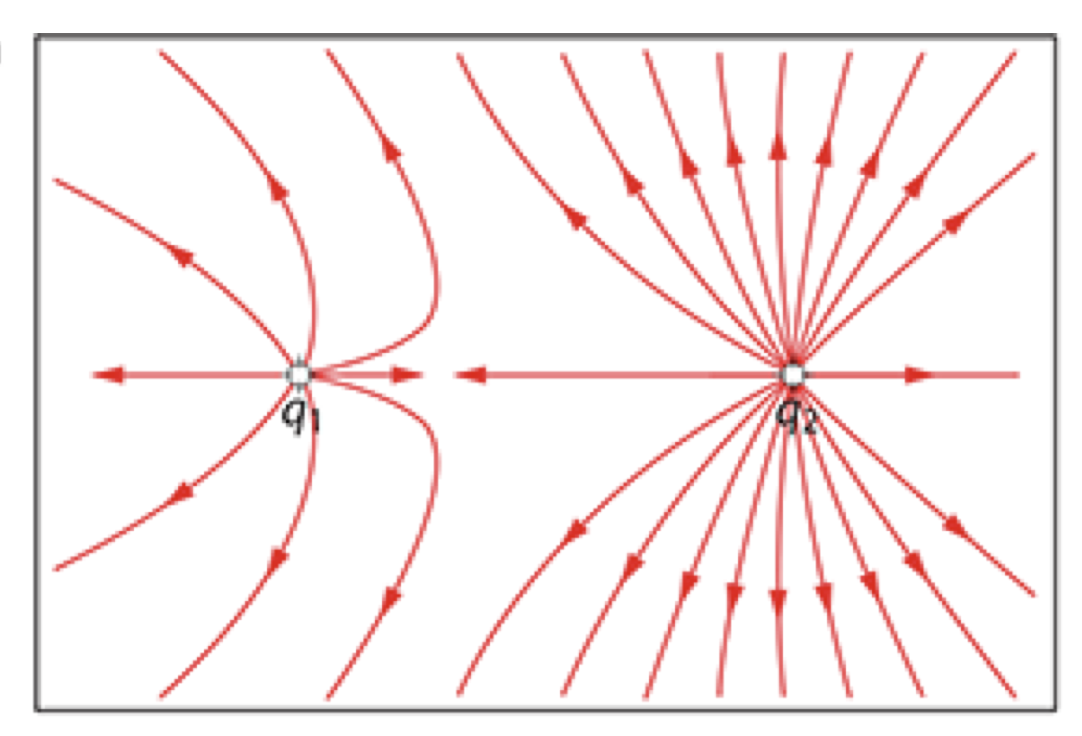
\includegraphics[width=0.3\linewidth]{Screenshot 2026-06-17 at 08.58.02.png}
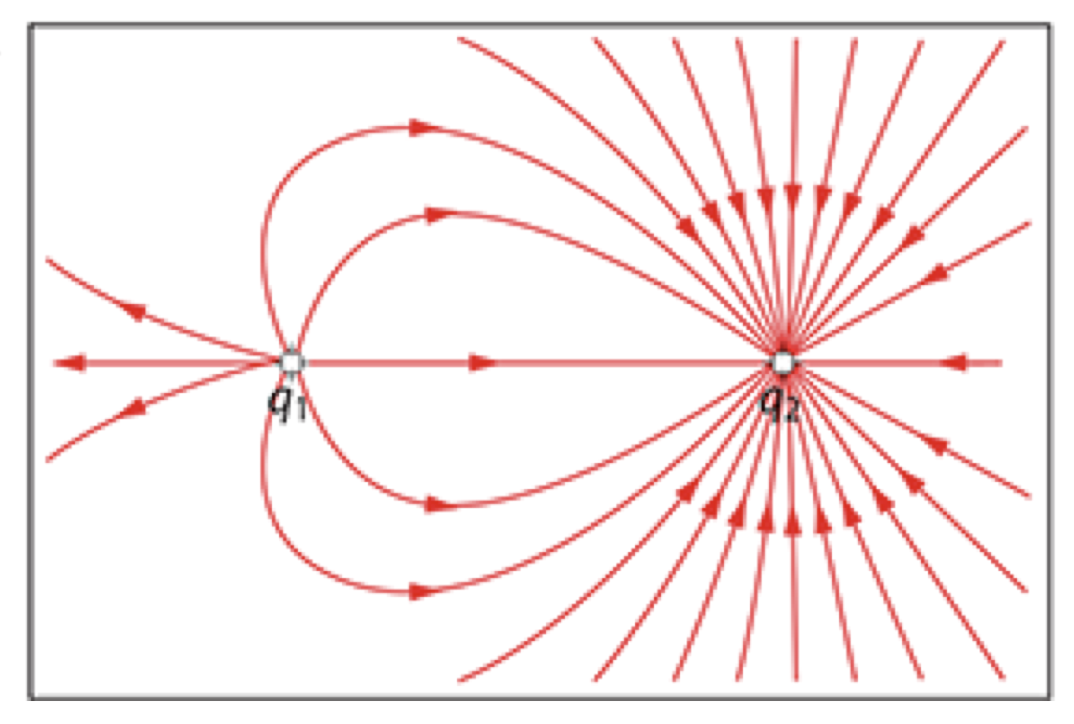
\includegraphics[width=0.3\linewidth]{Screenshot 2026-06-17 at 08.58.07.png}\\
Field lines for unequal and positive charges. Field lines for unequal and opposite charges.
\end{center}
\begin{center}
  \begin{tikzpicture}[>=Stealth, scale=1.0]

% =======================
% (a) Positive charge
% =======================
\node[font=\bfseries] at (0,4.2) {a};

\draw[thick,->]
(0,0) .. controls (0.2,1.5) and (0.8,2.6) .. (2.0,3.2);

\fill[blue] (0.15,1.0) circle (0.12);

\draw[red,very thick,->]
(0.15,1.0) -- ++(0.35,0.8);

\node[anchor=east] at (-0.2,2.0) {force};
\node[anchor=west] at (1.25,2.0) {field line};
\node[anchor=west] at (0.35,0.8) {positive charge};

% =======================
% (b) Negative charge
% =======================
\begin{scope}[xshift=6cm]

\node[font=\bfseries] at (0,4.2) {b};

\draw[thick,->]
(0,0) .. controls (0.2,1.5) and (0.8,2.6) .. (2.0,3.2);

\fill[red] (0.15,1.0) circle (0.12);

\draw[red,very thick,->]
(0.15,1.0) -- ++(-0.35,-0.8);

\node[anchor=east] at (-0.25,0.35) {force};
\node[anchor=west] at (1.25,2.0) {field line};
\node[anchor=west] at (0.35,0.8) {negative charge};

\end{scope}
\end{tikzpicture}
\end{center}
\begin{itemize}
  \item The electric force on a positive charge is tangent to the field line in the direction of the arrow of the field line.
  \item The force on a negative charge is tangent to the field line in a direction opposite to the arrow. 
\end{itemize}
\begin{center}
\begin{tikzpicture}[>=Stealth, scale=1.0]

    % Define colors
    \definecolor{platecolor}{RGB}{128,128,128}
    \definecolor{fieldred}{RGB}{220,50,50}
    \definecolor{fieldblue}{RGB}{100,150,220}

    % Top plate (positive)
    \fill[platecolor] (0.5, 2.5) rectangle (8.5, 3);

    % Bottom plate (negative)
    \fill[platecolor] (0.5, 0) rectangle (8.5, 0.5);

    % Positive charges on top plate
    \foreach \x in {1.5, 2.3, 3.1, 3.9, 4.7, 5.5, 6.3, 7.1, 7.9} {
        \node[fieldred, font=\Large] at (\x, 3.3) {+};
    }

    % Negative charges on bottom plate (using short dashes for minus signs)
    \foreach \x in {1.5, 2.3, 3.1, 3.9, 4.7, 5.5, 6.3, 7.1, 7.9} {
        \node[fieldblue, font=\large] at (\x, -0.3) {--};
    }

    % Electric field lines (vertical arrows from + to -)
    \foreach \x in {1.7, 2.5, 3.3, 4.1, 4.9, 5.7, 6.5, 7.3} {
        \draw[->, fieldred, thick] (\x, 2.4) -- (\x, 0.6);
    }

    % Distance marker 'd' with double-headed arrow
    \draw[<->, thick, black!70] (0.2, 0.5) -- (0.2, 2.5);
    \node[left] at (0.2, 1.5) {$d$};

    % Fringing field lines (curved lines at edges)
    % Left side - curved arrows
    \draw[->, fieldred, thick] plot[smooth, tension=0.7] coordinates {(0.5, 2.8) (0, 2.2) (-0.2, 1.5) (0, 0.8) (0.5, 0.2)};
    \draw[->, fieldred, thick] plot[smooth, tension=0.7] coordinates {(1, 2.9) (0.4, 2.3) (0.2, 1.5) (0.4, 0.7) (1, 0.1)};

    % Right side - curved arrows
    \draw[->, fieldred, thick] plot[smooth, tension=0.7] coordinates {(8.5, 2.8) (9, 2.2) (9.2, 1.5) (9, 0.8) (8.5, 0.2)};
    \draw[->, fieldred, thick] plot[smooth, tension=0.7] coordinates {(8, 2.9) (8.6, 2.3) (8.8, 1.5) (8.6, 0.7) (8, 0.1)};

    % Circuit connection to battery
    % Wire from top plate to battery positive
    \draw[thick] (8.5, 2.75) -- (10, 2.75);

    % Wire from bottom plate to battery negative
    \draw[thick] (8.5, 0.25) -- (10, 0.25);

    % Battery symbol
    % Positive terminal (longer line)
    \draw[thick, line width=2pt] (10, 2.5) -- (10, 3);
    % Negative terminal (shorter line)
    \draw[thick, line width=1pt] (10, 0) -- (10, 0.5);

    % Voltage label
    \node[right] at (10.3, 1.5) {$V$};

\end{tikzpicture}\\
The magnitude of the \textbf{uniform} electric field strength in between the plates is given by $E=\dfrac{V}{d}$.
\end{center}
\subsubsection*{The Millikan oil drop experiment}
\begin{center}
\begin{tikzpicture}[>=Stealth, scale=1.2]

    % Define colors
    \definecolor{platecolor}{RGB}{40,40,40}

    % Top plate (negative)
    \fill[platecolor] (0, 3) rectangle (5, 3.3);

    % Bottom plate (positive)
    \fill[platecolor] (0, 0) rectangle (5, 0.3);

    % Oil drop (blue circle)
    \fill[blue!60!cyan, draw=black, thick] (1.5, 1.65) circle (0.25);

    % Label "oil drop"
    \node[left, align=right] at (0.8, 1.65) {oil\\drop};

    % Upward force arrow (red) - electric force qE
    \draw[->, red!80!black, very thick] (1.5, 1.9) -- (1.5, 2.7);
    \node[right] at (1.65, 2.3) {$qE$};

    % Downward force arrow (black) - weight mg
    \draw[->, black, very thick] (1.5, 1.4) -- (1.5, 0.6);
    \node[right] at (1.65, 1.0) {$mg$};

\end{tikzpicture}
\end{center}
In this experiment, oil drops that were charged by X-rays were allowed to enter a region of uniform electric field between the parallel plates.
Some oil drops were observed to be at rest in between the plates. This means that the weight of the oil drop is matched by the electric force.
\[
\begin{aligned}
  mg&=qE\\
  mg&=q\dfrac{V}{d}\\
  &\Downarrow\\
  q&=\dfrac{mgd}{V}\\
\end{aligned}
\]
Millikan measured the mass of the oil drop by turning off the electric field and observed the oil drop that is now falling vertically down.
The oil drop quickly achieves terminal speed because now the weight is matched by the drag force given by Stoke's Law:\\
\[
\begin{aligned}
  mg&=6\pi\eta rv\\
  r&=\dfrac{mg}{6\pi\eta v}\\
  r&=\dfrac{\rho\left(\dfrac{4}{3}\pi r^3\right)g}{6\pi\eta v}\\
  r&=\sqrt{\dfrac{9\eta v}{2\rho g}}
\end{aligned}
\]
\begin{center}
  Find radius $\Rightarrow$ Find mass $\Rightarrow$ Find charge, is multiple of $e=1.6\times 10^{-19}\ \text{C}$
\end{center}
\subsection{Magnetic field and force}
A magnetic field is produced by electric currents. An electric field is produced by electric charges.
The vector representing a magnetic field is called magnetic flux density and its symbol is $B$.\\\\
In permanent magnets, such as bar magnets and horseshoe magnets, the magnetic field is created by microscopic currents due to the motion of electrons in the atoms of the material. These microscopic currents create microscopic magnetic fields; in materials called ferromagnetic these tiny fields are aligned so that a large observable macroscopic magnetic field is produced.
\begin{center}
  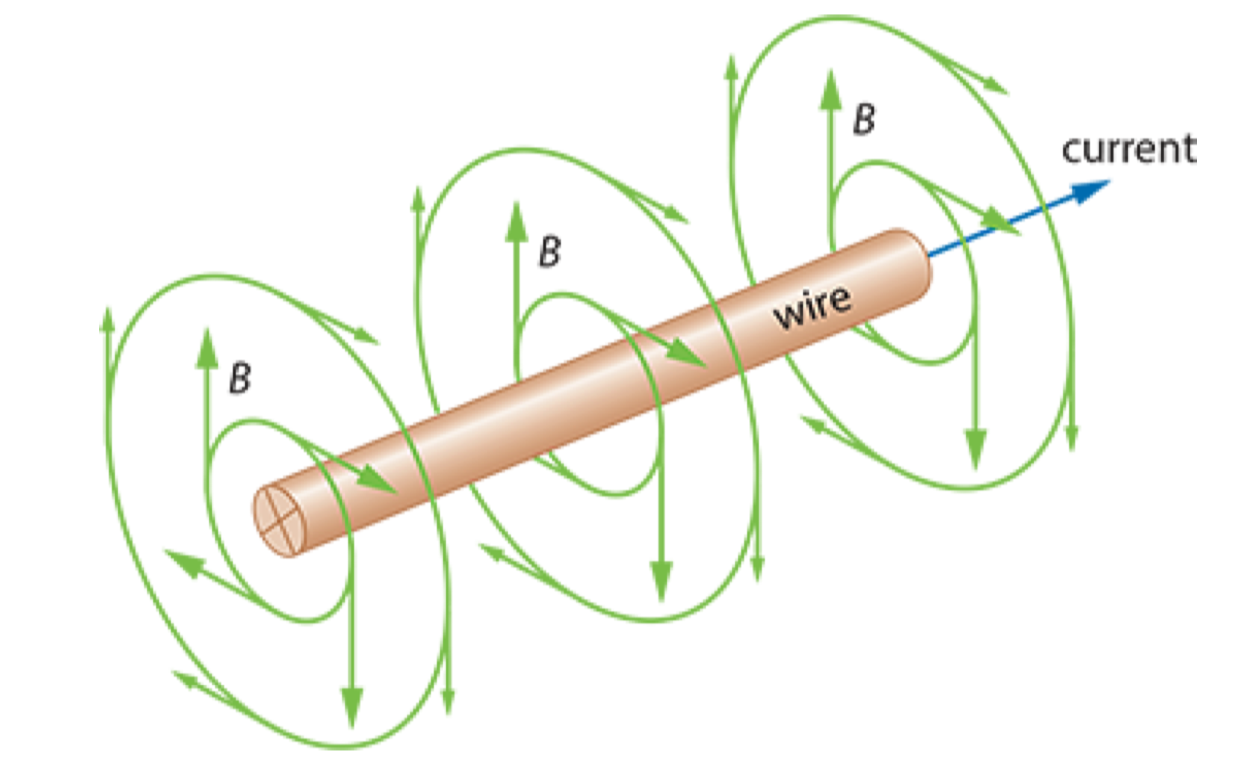
\includegraphics[width=0.4\linewidth]{Screenshot 2026-06-19 at 14.27.55.png}
  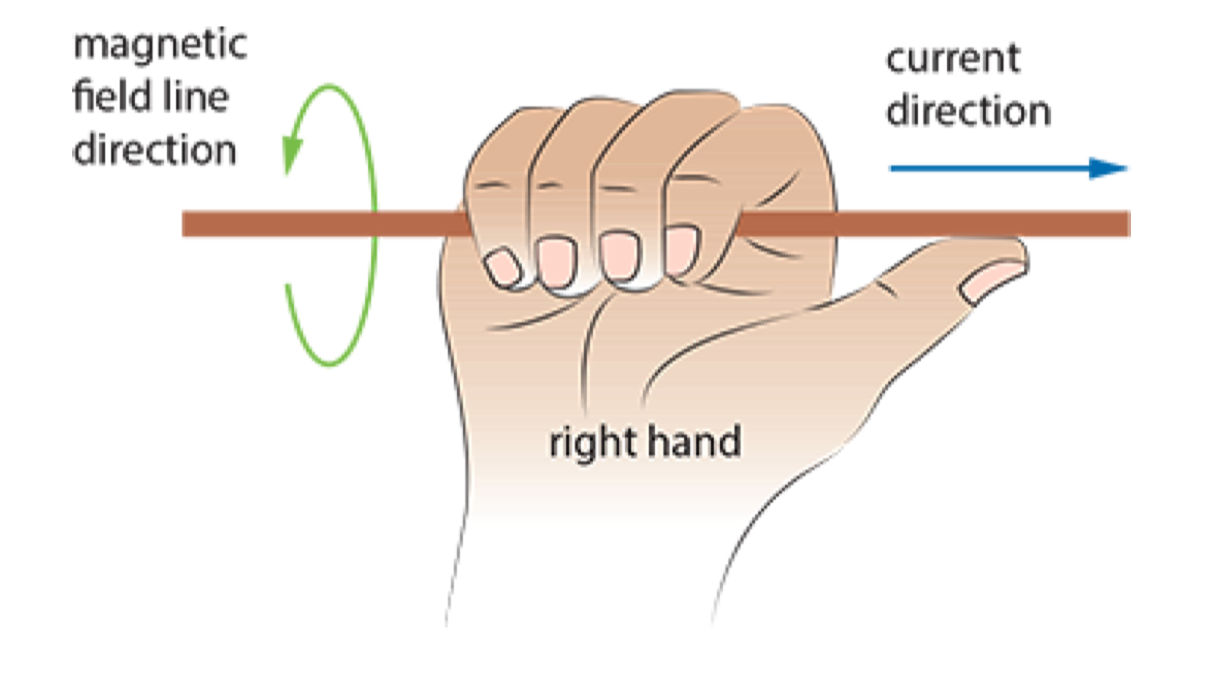
\includegraphics[width=0.4\linewidth]{Screenshot 2026-06-19 at 14.34.02.png}\\
\end{center}
\subsubsection*{Solenoids / coils}
The magnetic field lines within the solenoid are fairly uniform, indicating that the field is roughly constant in both magnitude and direction. Notice the similarity between the field outside the solenoid and that around the bar magnet. Notice also that magnetic field lines always exit from a north (N) pole and enter at a south (S) pole.
\begin{center}
  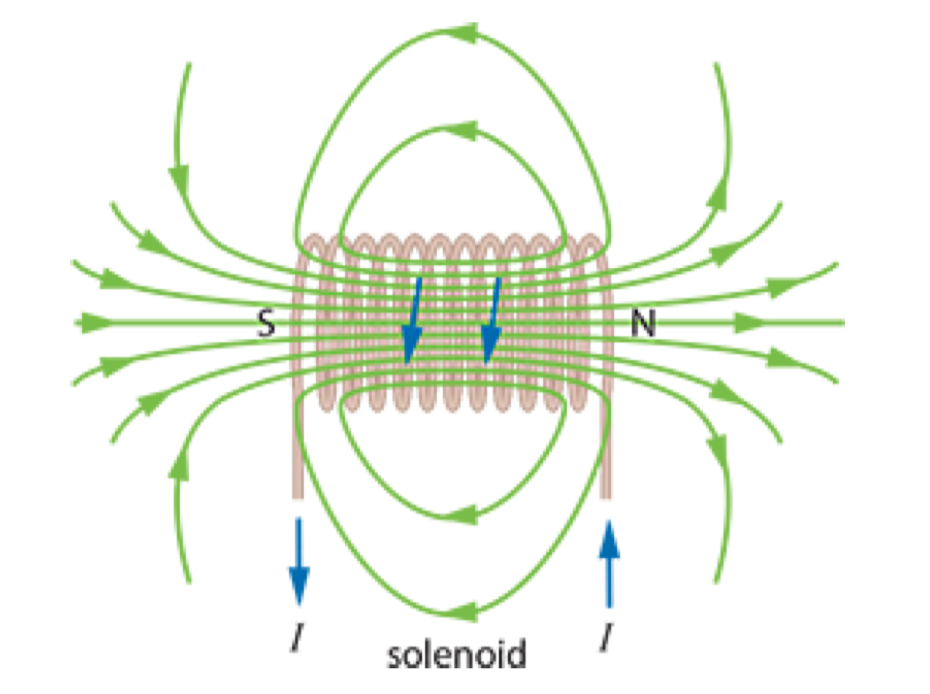
\includegraphics[width=0.4\linewidth]{Screenshot 2026-06-19 at 14.36.20.png}
  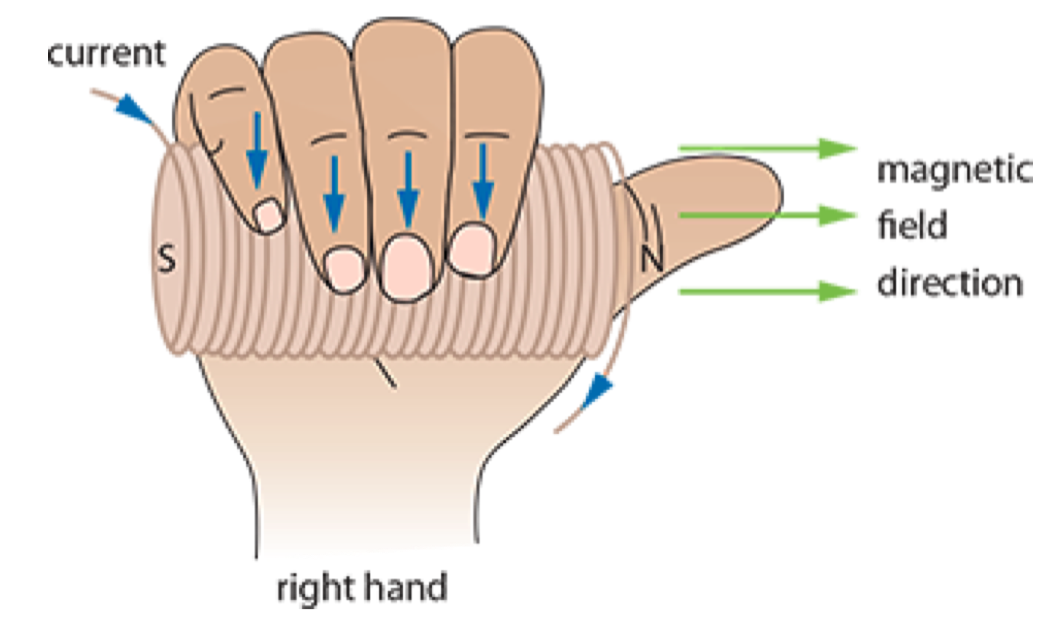
\includegraphics[width=0.4\linewidth]{Screenshot 2026-06-19 at 14.36.33.png}\\
\end{center}
\subsubsection*{The field of a single loop of current}
For all practical purposes the field of a ring, just like that in the exterior
of a coil, may be taken to be the same as that of a bar magnet.
\begin{center}
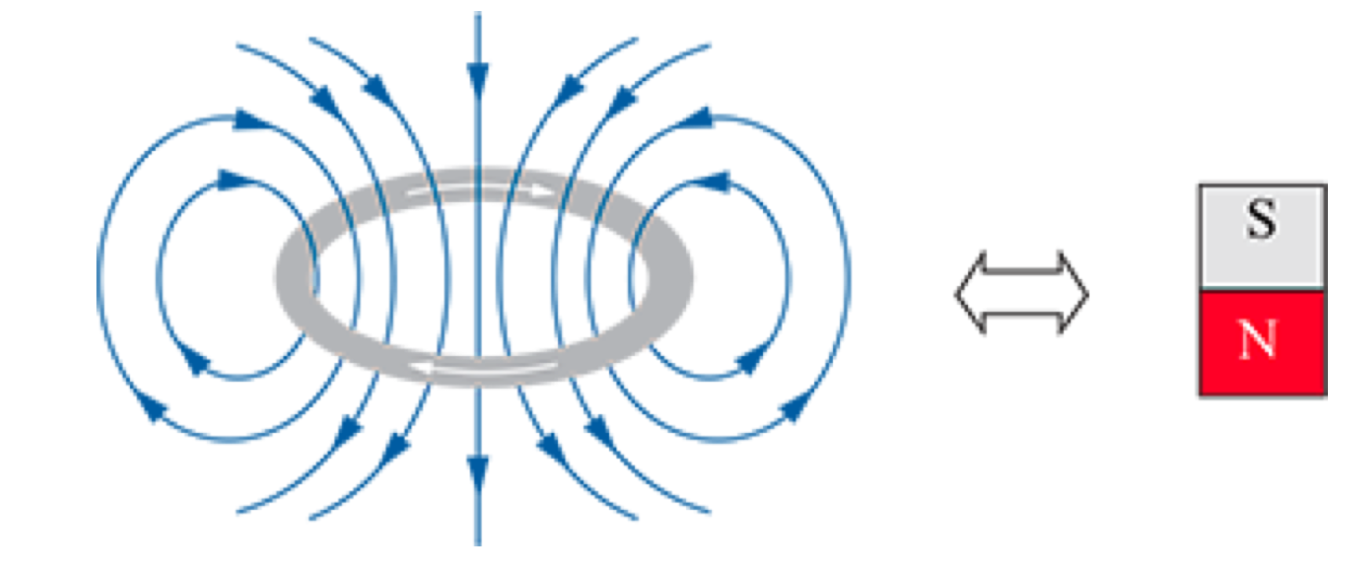
\includegraphics[width=0.6\linewidth]{Screenshot 2026-06-19 at 14.43.11.png}
\end{center}
\subsubsection*{Magnetic force on a moving charge}
Experiments show that an electric charge moving in a region of magnetic field experiences a new type of force called a magnetic force.
There is an exception to this rule: if the velocity of the charge is parallel to the direction of the field, the magnetic force is zero.\\\\
A charge $q$ moving with speed $v$ in a region of magnetic field of magnetic flux density $B$ will experience a magnetic force F given by:
\[F=qvB\sin\theta\]
Leave $\theta=90^\circ$ for most of the time, and $F=qvB$ would be obtained this way. The force is at right angles to both the velocity vector and the magnetic field. \textbf{Use left hand rule to find the direction of the force.}\\
Note that $\vec{F}=q\vec{v}\times \vec{B}$, the vector product of two. These rules give the direction of the magnetic force on a positive charge. To find the force on a negative charge, pretend the charge is positive and then reverse the force direction you find.\\
(Through this way, we can obtain the formula for magnetic flux density as $B=\dfrac{F}{qv\sin\theta}$. A magnetic flux density of 1 T produces a force of 1 N on a charge of 1 C moving at 1 m/s at right angles to the direction of the field.)\\
\begin{center}
  \begin{tikzpicture}[x=0.5cm,y=0.5cm,z=0.3cm,>=stealth,scale=0.7]
\draw[->] (xyz cs:x=0) -- (xyz cs:x=13.5) node[above] {Current $(I)$ (Direction of positive charge)};
\draw[->] (xyz cs:y=0) -- (xyz cs:y=13.5) node[right] {Force $(F)$};
\draw[->] (xyz cs:z=0) -- (xyz cs:z=13.5) node[above] {Magnetic Field $(B)$ (N to S)};
\end{tikzpicture}
\end{center}
\subsubsection*{The magnetic force on a current-carrying wire}
A current-carrying wire placed in a magnetic field will experience a magnetic force because there is a force on the moving charges in the wire.
The formula for the magnetic force on a length $L$ that finds itself in the region of the field is:
\[F=BIL\sin\theta\]
where $\theta$ is the angle between the current and the direction of the magnetic field.
\begin{center}
  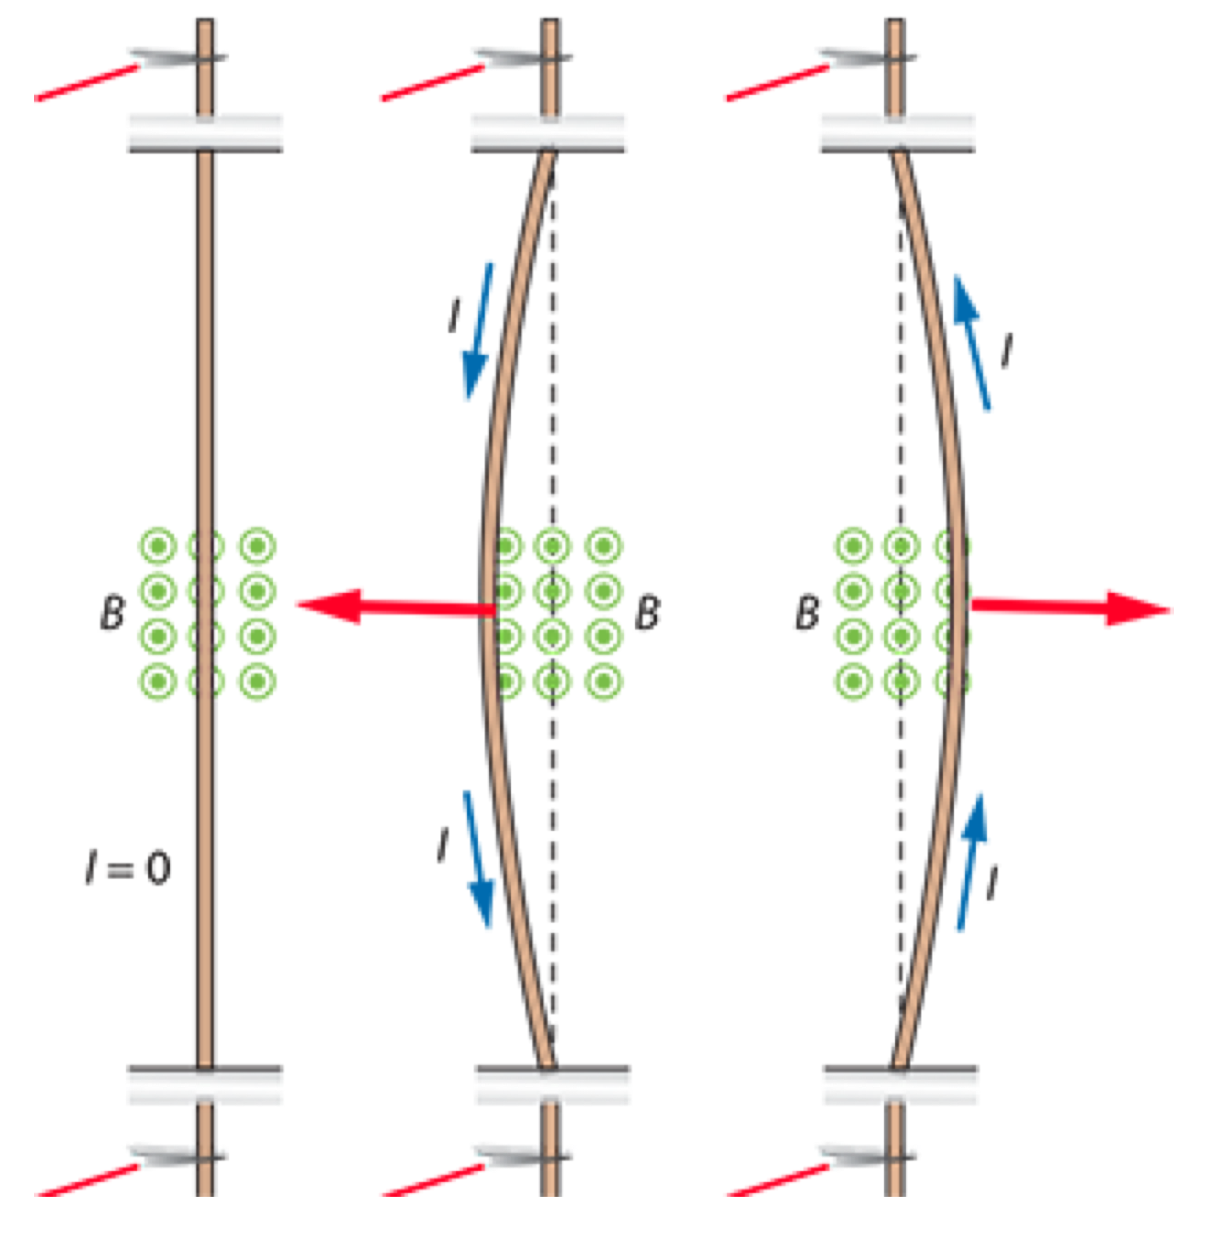
\includegraphics[width=0.5\linewidth]{Screenshot 2026-06-19 at 15.08.37.png}
\end{center}
\subsubsection*{The force between two current-carrying wires}
The currents are different in the two wires, so the magnetic fields are different, but the two forces are equal in magnitude.
(In the diagram below, $B_1\neq B_2$.) If the currents are parallel, the forces are attractive, and if they are anti-parallel, the forces are repulsive.
\begin{center}
  \begin{tikzpicture}[
    >=Stealth,
    force/.style={green!60!black,very thick,-{Stealth[length=4mm]}},
    field/.style={green!60!black,very thick,-{Stealth[length=4mm]}}
]

%----------------------------------------
% Helper symbols
%----------------------------------------
\newcommand{\crosswire}[2]{
    \draw (#1,#2) circle (0.35);
    \draw (#1-0.18,#2-0.18)--(#1+0.18,#2+0.18);
    \draw (#1-0.18,#2+0.18)--(#1+0.18,#2-0.18);
}

\newcommand{\dotwire}[2]{
    \draw (#1,#2) circle (0.35);
    \fill (#1,#2) circle (0.08);
}

%==================================================
% PARALLEL CURRENTS
%==================================================

\crosswire{0}{0}

\node[left] at (-0.45,0) {$I_1$};

\draw[field] (0,0) -- (0,1.6);
\node[left] at (-0.1,1.45) {$B_2$};

\draw[force] (0.4,0) -- (2.4,0);
\node at (1.4,0.35) {$F$};

\crosswire{5}{0}

\node[right] at (5.45,0) {$I_2$};

\draw[field] (5,0) -- (5,-1.6);
\node[right] at (5.15,-1.45) {$B_1$};

\draw[force] (4.6,0) -- (2.6,0);
\node at (3.6,0.35) {$F$};

\node at (2.5,1.2)
{parallel currents};

\begin{scope}[xshift=8cm]

\crosswire{1.5}{0}

\node[right] at (1.85,0) {$I_1$};

\draw[field] (1.5,0) -- (1.5,-1.6);
\node[right] at (1.65,-1.45) {$B_2$};

\draw[force] (1.1,0) -- (-1.0,0);
\node at (-0.15,0.35) {$F$};

\dotwire{4.5}{0}

\node[left] at (4.15,0) {$I_2$};

\draw[field] (4.5,0) -- (4.5,-1.6);
\node[right] at (4.65,-1.45) {$B_1$};

\draw[force] (4.9,0) -- (7.0,0);
\node at (6.1,0.35) {$F$};

\node at (3.0,1.2)
{anti-parallel currents};

\end{scope}

\end{tikzpicture}

\end{center}
\subsubsection*{Extension: Magnitude of Magnetic Flux density created}
 The magnitude of the magnetic flux density created at a distance $r$ from a long straight
wire carrying current $I$ is given by the formula $B=\dfrac{\mu_0I}{2\pi r}$, where $\mu_0=4\pi\times 10^{-7}\ \text{T\,m\,A}^{-1}$ is a constant of
physics called magnetic permeability. \\\\
The magnetic flux density
created by the left wire at the position of the right wire is $B_1=\dfrac{\mu_0I_1}{2\pi r}$. 
Therefore the force experienced by a length $L$ of the right wire is $F=B_1I_2L=\dfrac{\mu_0I_1I_2L}{2\pi r}$.\\
Thus, we can obtain the formula for force per unit length: $\dfrac{F}{L}=\mu_0\dfrac{I_1I_2}{2\pi r}$.
\subsection{Electric potential and electric potential energy}
An electric charge creates electric potential.
Two electric charges also share electric potential energy.
The formulas we derived for gravitation carry over to electricity essentially by replacing mass everywhere by charge.
\begin{center}
\begin{tikzpicture}[>=stealth, scale=0.95]
\definecolor{crimson}{rgb}{0.86, 0.08, 0.24}
\definecolor{forestgreen}{rgb}{0.13, 0.55, 0.13}
    % Define Styles
    \tikzstyle{massM} = [circle, draw=red!60!black, fill=red!70!brown, minimum size=2.4cm, line width=1.5pt]
    \tikzstyle{massm} = [circle, draw=red!60!black, fill=red!70!brown, minimum size=0.25cm, line width=1pt]

    % Coordinates
    \coordinate (M) at (0,0);
    \coordinate (m_near) at (4.5,0);
    \coordinate (m_mid) at (6.5,0);
    \coordinate (m_inf) at (9.5,0);

    % Draw Large Mass M
    \node[massM] at (M) {};
    \node[above=1.3cm] at (M) {$Q$};

    % Draw Mass m at Infinity
    \node[massm] (inf_node) at (m_inf) {};
    \node[above=0.2cm] at (inf_node) {$q$ at infinity};

    % Draw Mass m brought near to M
    \node[massm] (near_node) at (m_near) {};
    \node[above=0.2cm] at (near_node) {$q$ brought near to $Q$};

    % Draw connecting lines/arrows between the positions of m
    \draw[line width=1pt] (m_near) -- (m_mid);
    \draw[dashed, line width=1pt] (m_mid) -- (m_inf);

    % Red and Green Arrows on the near mass
    \draw[->, crimson, line width=1.5pt] (4.5,0) -- (5.6,0);
    \draw[->, forestgreen, line width=1.5pt] (7.6,0) -- (6.5,0);

    % Text label below the line
    \node[below=0.2cm] at (6.8,-0.1) {force does work};

    % Distance indicator r below the setup
    \def\yoffset{-1.4}
    \draw[<->, line width=0.8pt] (0,\yoffset) -- (4.5,\yoffset) node[midway, fill=white, inner sep=3pt] {$r$};

\end{tikzpicture}
\end{center}
The electric potential at a point P in an electric field is the amount of work done per unit charge as a small positive test charge q is moved from infinity to P: $V_e=\dfrac{W}{q}$.\\
The work done in moving a charge $q$ from infinity to point P is the electric potential energy of the system, $E_P=qV_e\left(=\dfrac{kQq}{r}\right)$. (Work done is expressed as $W=\dfrac{kQq}{r}$ by using calculus, therefore $V_e=\dfrac{kQ}{r}$. The value of $k=8.99\times 10^9$.)\\
Electric potential and electric potential energy are scalar quantities, just like gravitational potential and gravitational potential energy. The work done is independent of the path followed.\\
The work done W in moving charge q from A to B is: $W=q\Delta V_e$, where $\Delta V_e$ is the potential difference between A and B.\\
Electric potential is a scalar quantity. Therefore, if we have $i$ charges $q_i$ with distance of $r_i$ to the point P, then the electric potential at point P would be $V_e=\displaystyle k\sum \dfrac{q_i}{r_i}$.\\
For a point P outside the sphere and at a distance r from the centre of the sphere, the potential at P is $V_e=\dfrac{kQ}{r}$.\\
On the surface of the sphere the potential is $V_e=\dfrac{kQ}{R}$ where R is the radius of the sphere.\\
But at any point inside the sphere, the electric potential is constant and has the same value as the potential at the surface.\\\\
There is a deep connection between potential and field for both gravitation and electricity. To see this connection let us move a point charge q from a point P to a neighbouring point Q. There is a potential difference $\Delta V_e$ between the two points, and the points are a distance $\Delta$r apart.\\
$$W=qV_e=F\times d=qE\Delta r \Rightarrow E=\dfrac{\Delta V_e}{\Delta r}\left(-\dfrac{dV_e}{dr}\right)$$
In a graph showing the variation with distance of the potential, the gradient (slope) of the graph is the magnitude of the field strength. This applies to both gravitational and electric fields.
\subsubsection*{The connection between field lines and equipotential surfaces}
\begin{center}
Equipotential surfaces for a point charge.\\
\begin{tikzpicture}[
    >=Stealth,
    field/.style={blue!70, very thick, -{Stealth[length=3mm]}},
    equip/.style={gray!50, thick},
    scale=0.6
]

%=====================================
% (a) Equipotential surfaces
%=====================================

\begin{scope}

% central sphere
\fill[orange!90] (0,0) circle (0.65);

% equipotential circles
\foreach \r in {
0.95,1.15,1.35,1.55,1.75,
1.95,2.20,2.50,2.90,3.50}
{
    \draw[equip] (0,0) circle (\r);
}
\end{scope}

%=====================================
% (b) Equipotentials + field lines
%=====================================

\begin{scope}[xshift=8cm]

% sphere
\fill[orange!90] (0,0) circle (0.65);

% equipotential circles
\foreach \r in {
0.95,1.15,1.35,1.55,1.75,
1.95,2.20,2.50,2.90,3.50}
{
    \draw[equip] (0,0) circle (\r);
}

% radial field lines
\foreach \a in {0,30,60,90,120,150,180,210,240,270,300,330}
{
    \draw[field]
    ({4*cos(\a)},{4*sin(\a)})
    --
    ({0.7*cos(\a)},{0.7*sin(\a)});
}

% labels
\node[align=center] at (-1.8,4.7)
{equipotential};

\draw[black]
(-1.6,4.2) -- (-1.3,2.8);

\node at (3.2,4.7)
{field line};

\draw[black]
(2.8,4.2) -- (2.1,2.6);

\end{scope}

\end{tikzpicture}\\The field lines are at right angles to the equipotential surfaces.
\end{center}
Explanation for why field lines are at right angles to the equipotential surfaces:\\
To move a charge from one point on an equipotential surface to another requires zero work. If the field lines were not normal to the equipotential surfaces, there would be a component of the field along the equipotential and so a force on the charge. As the charge moved this force would do work, which contradicts the fact that the work should be zero.
\begin{center}
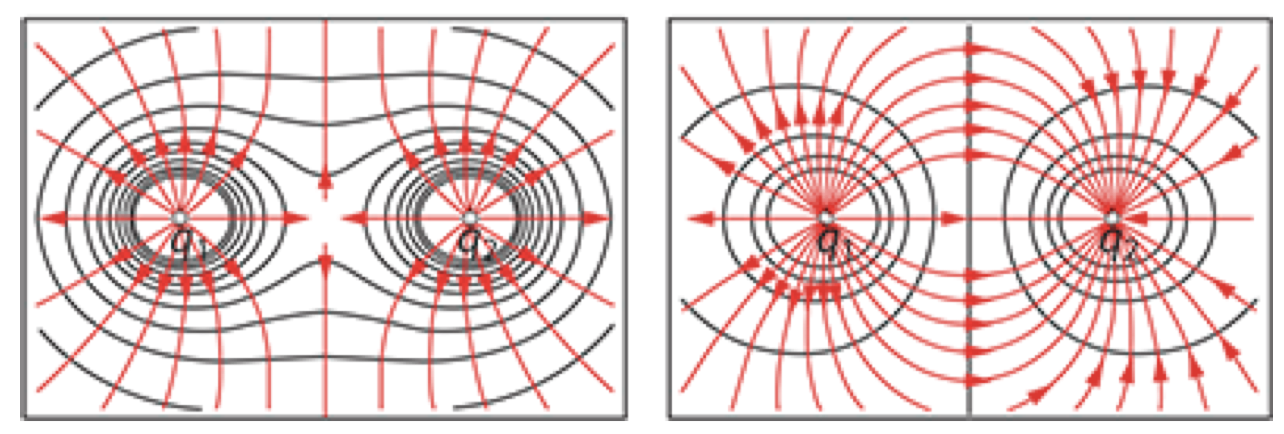
\includegraphics[width=0.45\linewidth]{Screenshot 2026-06-26 at 17.04.52.png}
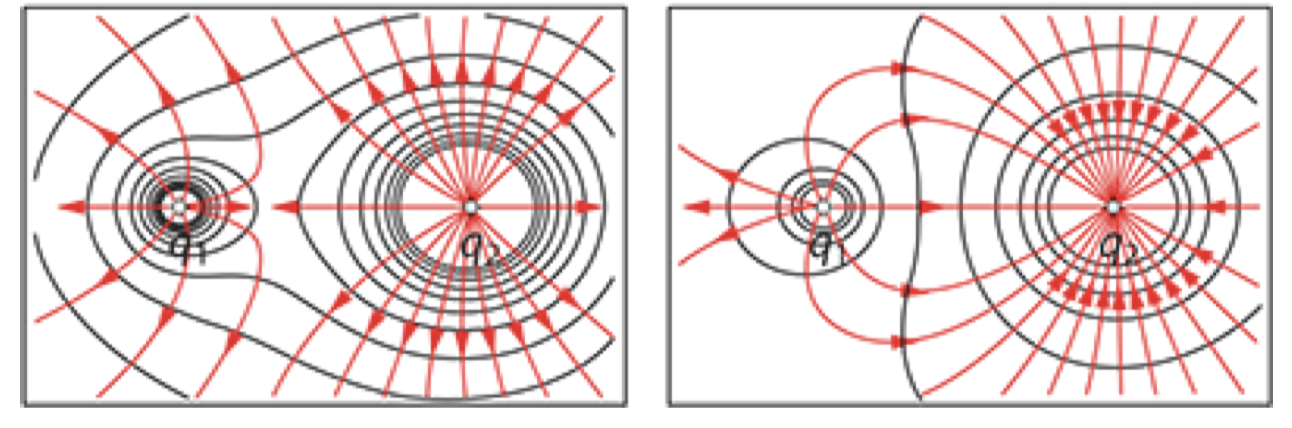
\includegraphics[width=0.45\linewidth]{Screenshot 2026-06-26 at 17.05.09.png}
\\
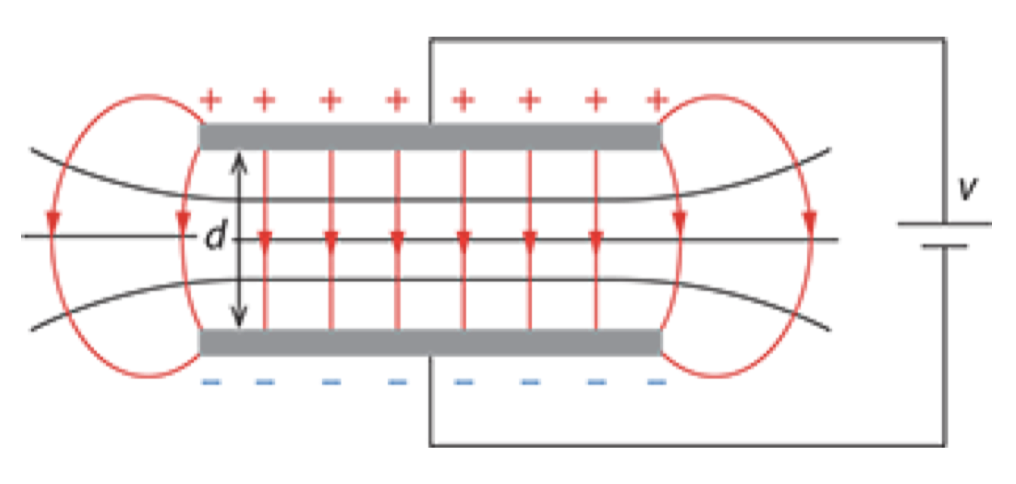
\includegraphics[width=0.4\linewidth]{Screenshot 2026-06-26 at 17.02.09.png}
\end{center}
\section{Motion in electric and magnetic fields}
\subsection{Motion in an electric field}
The path of an electric charge in a uniform electric field is either a straight line or a parabolic path. We have a straight line if the charge is initially at rest or if its original velocity is parallel to the electric field. In all other cases we have a parabolic path.\\
A positive particle will experience a force $qE$ in the direction of the field. It will also accelerate in the direction of the field, $a=\dfrac{qE}{m}$.\\
The positive charge increases its kinetic energy (= work done by eletric force, $qV$) as it moves to the right.
\begin{center}
  \begin{minipage}{0.48\textwidth}
    \centering
    \begin{tikzpicture}[>=Stealth, scale=1.1]
      % Horizontal Blue Electric Field Lines
      \foreach \y in {-1, 0, 1} {
        \draw[blue!80!black, stroke, thick, ->] (0.5, \y) -- (5.5, \y);
      }
      \node[black] at (4.8, 0.3) {$E$ field};
      
      % Vertical Red Dotted Lines
      \draw[red, dotted, thick] (1.7, -1.5) -- (1.7, 1.5);
      \draw[red, dotted, thick] (4.2, -1.5) -- (4.2, 1.5);
      
      % Labels X and Y
      \node[above] at (1.7, 1.5) {X};
      \node[above] at (4.2, 1.5) {Y};
      
      % Green Force Arrow
      \draw[green!60!black, ->, ultra thick] (1.7, 0) -- (2.9, 0) node[above, midway, black] {$F = qE$};
      
      % Charged Particle
      \filldraw[fill=blue!70!black, draw=black, thick] (1.7, 0) circle (3.5pt);
      \node[above left] at (1.7, 0) {$q$};
    \end{tikzpicture}
  \end{minipage}
  % --- SECOND IMAGE (Right) ---
  \begin{minipage}{0.48\textwidth}
    \centering
    \begin{tikzpicture}[>=Stealth, scale=1.1]
      % Axis indicators on the far left
      \draw[->, thick] (-0.6, 0.5) -- (0.0, 0.5) node[above] {$x$};
      \draw[->, thick] (-0.6, 0.5) -- (-0.6, -0.1) node[left] {$y$};
      
      % Vertical Blue Electric Field Lines
      \foreach \x in {0.5, 1.5, 2.5, 3.5, 4.5} {
        \draw[blue!80!black, thick, ->] (\x, 1.3) -- (\x, -1.7);
      }
      
      % Horizontal Red Dotted Lines
      \draw[red, dotted, thick] (0.2, 0.5) -- (4.8, 0.5);
      \draw[red, dotted, thick] (0.2, -0.4) -- (4.8, -0.4);
      
      % Vertical Displacement Double Arrow (y)
      \draw[<->, thick] (4.7, 0.5) -- (4.7, -0.4) node[right, midway] {$y$};
      
      % Green Parabolic Trajectory
      % Equation: y = 0.5 - 0.1*(x - 0.5)^2
      \draw[green!60!black, thick, domain=0.5:4.6, samples=50] plot (\x, {0.5 - 0.1*(\x-0.5)^2});
      
      % First Position (Initial Entry)
      \filldraw[fill=blue!70!black, draw=black, thick] (0.5, 0.5) circle (3pt);
      \draw[red, ->, ultra thick] (0.5, 0.5) -- (1.3, 0.5) node[above, midway, black] {$u$};
      
      % Second Position (Deflected Point along the 4th line)
      % At x = 3.5, y = 0.5 - 0.1*(3.0)^2 = -0.4
      \filldraw[fill=blue!70!black, draw=black, thick] (3.5, -0.4) circle (3pt);
      \draw[red, ->, ultra thick] (3.5, -0.4) -- (4.3, -0.4); % Horizontal velocity component
      \draw[red, ->, ultra thick] (3.5, -0.4) -- (3.5, -1.3); % Vertical velocity component
    \end{tikzpicture}
  \end{minipage}
\end{center}
In the second figure:
\begin{itemize}
  \item the particle will follow a parabolic path
  \item the component of velocity normal to the field will remain constant: $v_x=u$
  \item the component of velocity parallel to the field will increase uniformly: $v_y=\dfrac{qE}{m}t$
  \item The kinetic energy of the particle increases as time goes on because the electric force is doing work on the particle.
  \item After time $t$, the particle will move a horizontal distance $x = ut$ and fall a vertical distance $y = \dfrac{1}{2}\dfrac{qE}{m}t^2$.
  \item $$ 
  \begin{aligned}
   E_K&= \dfrac{1}{2}mv^2\\
    &= \dfrac{1}{2}m\left(v_x^2+v_y^2\right)\\
    &= \dfrac{1}{2}m\left(u^2+\left(\dfrac{qE}{m}t\right)^2\right)
  \end{aligned} $$ 
  \item $\therefore \Delta E_K=\dfrac{1}{2}m\left(\dfrac{qEt}{m}\right)^2=Fy$, work done by the electric force.
\end{itemize}
Equations involved in trajectory in Chapter 1 also applies here. 
\subsection{Motion in a magnetic field}
\begin{itemize}
  \item In the simple case where the velocity of the charged particle is parallel or anti-parallel to that of the uniform magnetic field, the magnetic force is zero and so the particle will move along a straight line.
  \item A positive charge in a uniform magnetic field that is directed into the plane of the paper. The velocity is at right angles to the magnetic field. The magnetic force is at right angles to both the velocity and the magnetic field so the particle will follow a circular path; the centripetal force is provided by the magnetic force.\\
  Radius $R=\dfrac{mv}{qB}$, time to make one complete revolution $T=\dfrac{2\pi m}{qB}$ (independent of the speed).
  \item If the positively charged particle loses energy as it moves along the circular path, the speed will decrease, and from the formula for the radius we see that the radius will also decrease. This means that the circular path will become a spiral.
\end{itemize}
\begin{center}
  \begin{tikzpicture}[x=1cm, y=1cm, scale=0.6]
  % Define colors for use
  \definecolor{mygreen}{rgb}{0,0.5,0}

  % Draw Green B Field Lines (Arrows pointing down, cover the diagram)
  \foreach \x in {1, 4, 6, 9.5} {
    \draw[mygreen, thick, ->] (\x, 10) -- (\x, 1);
  }

  % Draw Left Particle System
  % Dashed line first (behind the rest)
  \draw[dashed, gray, thin] (2.5, 2) -- (2.5, 7);
  % Red force arrow pointing up
  \draw[red, ultra thick, ->, >=stealth] (2.5, 3) -- (2.5, 6);
  % Blue particle node
  \draw[fill=blue, draw=black, thick] (2.5, 3) circle (3mm);

  % Draw Right Particle System
  % Dashed line first
  \draw[dashed, gray, thin] (7.5, 4) -- (7.5, 9);
  % Red force arrow pointing down
  \draw[red, ultra thick, ->, >=stealth] (7.5, 8) -- (7.5, 5);
  % Blue particle node
  \draw[fill=blue, draw=black, thick] (7.5, 8) circle (3mm);
\end{tikzpicture}
\hfill 
\begin{tikzpicture}[>=Stealth, scale=1.2]
  % Define colors to match the image accurately
  \definecolor{fieldgreen}{rgb}{0.55, 0.78, 0.42}  % Light green for B-field indicators
  \definecolor{forcegreen}{rgb}{0.24, 0.65, 0.41}  % Darker green for the force vector
  \definecolor{velored}{rgb}{0.85, 0.23, 0.18}     % Vivid red for velocity vector
  
  % Draw uniform magnetic field (6 columns x 5 rows of circled crosses)
  \foreach \x in {2,3,4,5,6} {
    \foreach \y in {1,2,3,4,5} {
      % Outer circle
      \draw[fieldgreen, ultra thick] (\x,\y) circle (0.16);
      % Inner cross (X)
      \draw[fieldgreen, ultra thick] (\x-0.1, \y-0.1) -- (\x+0.1, \y+0.1);
      \draw[fieldgreen, ultra thick] (\x-0.1, \y+0.1) -- (\x+0.1, \y-0.1);
    }
  }
  
  % Define geometry of the circular orbit
  \coordinate (Center) at (4,3);
  \def\R{2.15}      % Radius of the trajectory
  \def\Angle{38}    % Angular position of the particle
  
  % Draw the black circular trajectory
  \draw[black, thick] (Center) circle (\R);
  
  % Calculate the exact position of the particle
  \coordinate (P) at ($(Center) + (\Angle:\R)$);
  
  % Draw the Centripetal Force Vector (pointing directly to the center)
  \draw[forcegreen, ->, ultra thick] (P) -- (Center);
  \node[right, font=\large\itshape, xshift=5pt, yshift=5pt] at (Center) {F};
  
  % Draw the Tangential Velocity Vector (perpendicular to the radius, pointing up-left)
  \draw[velored, ->, ultra thick] (P) -- ($(P) + ({\Angle+90}:1.2)$);
  \node[right, font=\large\itshape, xshift=2pt, yshift=2pt] at ($(P) + ({\Angle+90}:1.2)$) {v};
  
  % Draw the charged particle on top
  \filldraw[fill=black, draw=black] (P) circle (2.5pt);

\end{tikzpicture}
\hfill
\begin{tikzpicture}[>=Stealth, scale=1.5]

% --- Green Magnetic Field Indicators (B-field) ---
% Define a custom command to draw the circled 'X' symbol for field pointing into the page
\newcommand{\BfieldX}[1]{
    \draw[green!70!black, thick] (#1) circle (0.08); 
    \draw[green!70!black, thin] (#1)+(-0.05,-0.05) -- (#1)+(0.05,0.05); 
    \draw[green!70!black, thin] (#1)+(-0.05,0.05) -- (#1)+(0.05,-0.05);
}

% Draw a uniform grid of B-field symbols
\foreach \x in {-1.5, 0, 1.5} {
    \foreach \y in {-1.5, 0, 1.5} {
        \BfieldX{\x,\y};
    }
}

% --- Blue Spiral Path ---
% Draw an outward, clockwise expanding spiral in blue
\draw[blue!70!black, thick, smooth, samples=200, domain=0:8.5*pi] 
    plot ( {-1*(\x r)} : {0.07*\x} );

% --- Particle and Velocity Vector ---
% Particle (red dot), placed visually inside the outer grid points
\fill[red] (1.76, 0) circle (0.04);

% Velocity Vector (red arrow), pointing down and to the right from the particle
\draw[red, thick, ->] (1.76, 0) -- (1.7, -1);

\end{tikzpicture}
\end{center}
\subsubsection*{Work done and magnetic forces}
Since the magnetic force is always normal to the velocity of the charge, it follows that it cannot do any work. This means the kinetic energy of the particle cannot change while in the region of magnetic field.
\subsubsection*{Motion in crossed electric and magnetic fields}
\begin{itemize}
  \item If two forces are equal, the particle will continue moving on a straight line undeflected from its original path, $E=vB$.
  \item If the particle enters with speed greater than $v=\dfrac{E}{B}$, the particle will move upwards (larger $F_m$). 
  \item If the speed is less than $v$, the particle will move downwards.
\end{itemize}
\begin{center}
  \begin{tikzpicture}[>=stealth, font=\small, scale=1.25]
% Define custom colors based on the image
\definecolor{efieldblue}{RGB}{30, 144, 255} % A clear, vibrant blue for E field lines and labels
\definecolor{bfieldgreen}{RGB}{124, 184, 100} % A soft, natural green for B field markers and labels
\definecolor{velocityred}{RGB}{230, 50, 50} % A clear, sharp red for the velocity vector
% --- MAIN FIELD REGION ---

% Spacing for the B-field grid
\def\gx{1.6}
\def\gy{1.6}

% Draw the 3x3 grid of B-field (into page) markers
\foreach \x [evaluate=\x as \evalx using \x*\gx] in {0, 1, 2} {
  \foreach \y [evaluate=\y as \evaly using \y*\gy] in {0, 1, 2} {
    
    % We pass just the raw coordinates. No extra parentheses, no inline math!
    \BInto{\evalx, \evaly}
    
  }
}
% Draw the 5 vertical E-field arrows
\def\Lx{0.8} % Shift for lines to be interspersed with markers
\foreach \xi in {0.5, 1.5, 2.5, 3.5} {
  \draw[efieldblue, ->, thick] (\xi*\Lx, 3.6) -- (\xi*\Lx, 0);
}

% Draw the particle and its velocity vector in the field area
\coordinate (P1) at (-0.3, 2.5); % Positioned visually near the top-left B marker
\fill[efieldblue, draw=black, thick] (P1) circle (0.11cm);
\draw[velocityred, ->, thick] (P1) -- ++(1.6, 0);
\node[anchor=south, color=velocityred] at ($(P1) + (0.8, 0)$) {$v$};

% Add the E-field and B-field text labels
\node[efieldblue, anchor=south west] at (1.9, -0.8) {E field};
\node[bfieldgreen, anchor=south east] at (4.6, 3.2) {B field};
\end{tikzpicture}
\begin{tikzpicture}[>=stealth, scale=1.5]
  \definecolor{efieldblue}{RGB}{30, 144, 255} % A clear, vibrant blue for E field lines and labels
\definecolor{bfieldgreen}{RGB}{124, 184, 100} % A soft, natural green for B field markers and labels
% Spacing for the FBD, clearly separated but visually related
\def\fbdx{0}
\coordinate (P2) at (\fbdx, 2.5);

% Draw the particle in the FBD
\fill[efieldblue, draw=black, thick] (P2) circle (0.11cm);

% Draw the Magnetic Force arrow (upward) and its label
\draw[bfieldgreen, ->, thick] (P2) -- ++(0, 1.6);
\node[bfieldgreen, anchor=east] at ($(P2) + (-0.1, 1.2)$) {$qvB$};

% Draw the Electric Force arrow (downward) and its label
\draw[efieldblue, ->, thick] (P2) -- ++(0, -1.4);
\node[efieldblue, anchor=north] at ($(P2) + (0, -1.4)$) {$qE$};

\end{tikzpicture}
\end{center}
\section{Electromagnetic induction}
\subsection{Electromagnetic induction}
\subsubsection*{Motional $e.m.f$}
\begin{center}
  \begin{tikzpicture}[>=Stealth, scale=1]

  % --- Color Definitions ---
  \definecolor{fieldgreen}{RGB}{137, 194, 103}    % Soft green for B-field circles
  \definecolor{forcegreen}{RGB}{46, 150, 91}      % Darker green for Force vector
  \definecolor{velocityred}{RGB}{220, 60, 50}     % Vivid red for Velocity vector
  \definecolor{rodpeach}{RGB}{246, 214, 199}      % Light peach for the conductor rod

  % --- 1. Background Uniform Magnetic Field (8 columns x 6 rows) ---
  \foreach \x in {1, 2, 3, 4, 5, 6, 7, 8} {
    \foreach \y in {1, 2, 3, 4, 5, 6} {
      % Circle
      \draw[fieldgreen, thick] (\x, \y) circle (0.13);
      % Inner Cross (X)
      \draw[fieldgreen, thin] (\x-0.08, \y-0.08) -- (\x+0.08, \y+0.08);
      \draw[fieldgreen, thin] (\x-0.08, \y+0.08) -- (\x+0.08, \y-0.08);
    }
  }

  % --- 2. Moving Conductor Rod ---
  % Placed cleanly between columns 3 and 4
  \draw[draw=black!40, fill=rodpeach, thick] (3.2, 1.4) rectangle (3.8, 5.6);

  % Charge Accumulation Labels (+ at top, - at bottom)
  \node[font=\bfseries, yshift=6pt] at (3.5, 5.6) {$+\,\,+\,\,+$};
  \node[font=\bfseries, yshift=-7pt] at (3.5, 1.4) {$-\,\,-\,\,-$};

  % --- 3. Length Dimension Indicator (L) ---
  \draw[<->, black, thick] (2.9, 1.4) -- (2.9, 5.6);
  \node[left, font=\large\itshape] at (2.9, 3.5) {L};

  % --- 4. Force Vector Inside the Rod (F) ---
  \draw[forcegreen, ->, ultra thick] (3.5, 5.2) -- (3.5, 2.3);
  \node[below, font=\large\itshape, yshift=-2pt] at (3.5, 2.3) {F};

  % --- 5. Velocity Vector (v) ---
  \draw[velocityred, ->, ultra thick] (3.8, 3.5) -- (7.4, 3.5);
  \node[right, font=\large\itshape, xshift=3pt] at (7.4, 3.5) {v};

\end{tikzpicture}
\end{center}
The rod is conducting. As it moves, the electrons within it also move from left to right. The magnetic field will exert a force on these moving electrons. The force on the electrons is directed downward.
This means that the lower end of the rod has a net negative charge and the top end has an equal net positive charge. The flow of electrons towards the bottom end of the rod will stop when the electrons already there are numerous enough to push any new electrons back by electrostatic repulsion. There is, in other words, an electric field established in the rod whose direction is from top to bottom.\\\\
$E=\dfrac{\varepsilon}{L}$, where $\varepsilon$ is the induced $e.m.f$ and $L$ is the length of the rod. The induced $e.m.f$ is given by $\varepsilon=BLv$.
It is important to note that except for a very short interval of time initially, no current exists in the rod. 
\begin{center}
  \begin{tikzpicture}[>=Stealth, scale=1.1]

  % --- Color Definitions ---
  \definecolor{fieldgreen}{RGB}{137, 194, 103}    % Soft green for B-field circles
  \definecolor{velocityred}{RGB}{220, 60, 50}     % Vivid red for Velocity vector
  \definecolor{rodpeach}{RGB}{246, 214, 199}      % Light peach for the conductor rod

  % --- 1. Background Uniform Magnetic Field (7 columns x 5 rows) ---
  \foreach \x in {1, 2, 3, 4, 5, 6, 7} {
    \foreach \y in {1, 2, 3, 4, 5} {
      \draw[fieldgreen, thick] (\x, \y) circle (0.13);
      \draw[fieldgreen, thin] (\x-0.08, \y-0.08) -- (\x+0.08, \y+0.08);
      \draw[fieldgreen, thin] (\x-0.08, \y+0.08) -- (\x+0.08, \y-0.08);
    }
  }

  % --- 2. Circuit Rails and Resistor ---
  % Top Rail (placed perfectly between row 4 and row 5 of the field)
  \draw[black, very thick] (1.5, 4.5) -- (7.5, 4.5);
  % Bottom Rail (placed perfectly between row 1 and row 2 of the field)
  \draw[black, very thick] (1.5, 1.5) -- (7.5, 1.5);
  
  % Vertical wire connecting the rails on the left side
  \draw[black, very thick] (1.5, 1.5) -- (1.5, 4.5);
  
  % Resistor R component container
  \draw[black, fill=white, thick] (1.32, 2.6) rectangle (1.68, 3.4);
  \node[left, font=\large\itshape, xshift=-2pt] at (1.32, 3.0) {R};

  % --- 3. Sliding Conductor Rod ---
  % Centered safely between column 3 and column 4 (at x = 3.5)
  \draw[draw=black!40, fill=rodpeach, thick] (3.3, 1.5) rectangle (3.7, 4.5);

  % --- 4. Labels and Surface Charges ---
  % "top" and "bottom" boundary text labels
  \node[font=\large] at (4.5, 5.5) {top};
  \node[font=\large] at (4.5, 0.5) {bottom};

  % Positive charges along the upper rail surface
  \node[anchor=south, font=\footnotesize, yshift=-1pt] at (4.5, 4.5) 
    {$+\,\,+\,\,+\,\,+\,\,+\,\,+\,\,+\,\,+\,\,+\,\,+\,\,+\,\,+\,\,+\,\,+\,\,+$};

  % Negative charges along the lower rail surface
  \node[anchor=north, font=\footnotesize, yshift=2pt] at (4.5, 1.5) 
    {$\scalebox{0.8}[1.0]{$-$}\,\,\scalebox{0.8}[1.0]{$-$}\,\,\scalebox{0.8}[1.0]{$-$}\,\,\scalebox{0.8}[1.0]{$-$}\,\,\scalebox{0.8}[1.0]{$-$}\,\,\scalebox{0.8}[1.0]{$-$}\,\,\scalebox{0.8}[1.0]{$-$}\,\,\scalebox{0.8}[1.0]{$-$}\,\,\scalebox{0.8}[1.0]{$-$}\,\,\scalebox{0.8}[1.0]{$-$}\,\,\scalebox{0.8}[1.0]{$-$}\,\,\scalebox{0.8}[1.0]{$-$}\,\,\scalebox{0.8}[1.0]{$-$}\,\,\scalebox{0.8}[1.0]{$-$}\,\,\scalebox{0.8}[1.0]{$-$}\,\,\scalebox{0.8}[1.0]{$-$}$};

  % --- 5. Velocity Vector (v) ---
  % Originates cleanly from the right side of the moving rod
  \draw[velocityred, ->, ultra thick] (3.7, 3.0) -- (6.8, 3.0);
  \node[right, font=\large\itshape, xshift=3pt] at (6.8, 3.0) {v};

\end{tikzpicture}
\end{center}
Now there exists a current of $I=\dfrac{BvL}{R}$ in the circuit, and the moving rod behaves as a battery. In this diagram the current is going counterclockwise. \\
Notice also that now that we have a current, the rod needs to be pushed if it is to continue to move at constant speed. Now it's experiencing a magnetic force of $F=\dfrac{vB^2L^2}{R}$ directed to the left.\\
For speed to remain constant a force of equal magnitude needs to act on the rod, directed to the right. The power $P$ generated by this force $=\dfrac{(BvL)^2}{R}$, consistent with the power dissipated in the circuit as thermal energy.
\subsubsection*{Magnetic flux and magnetic linkage}
\begin{center}
  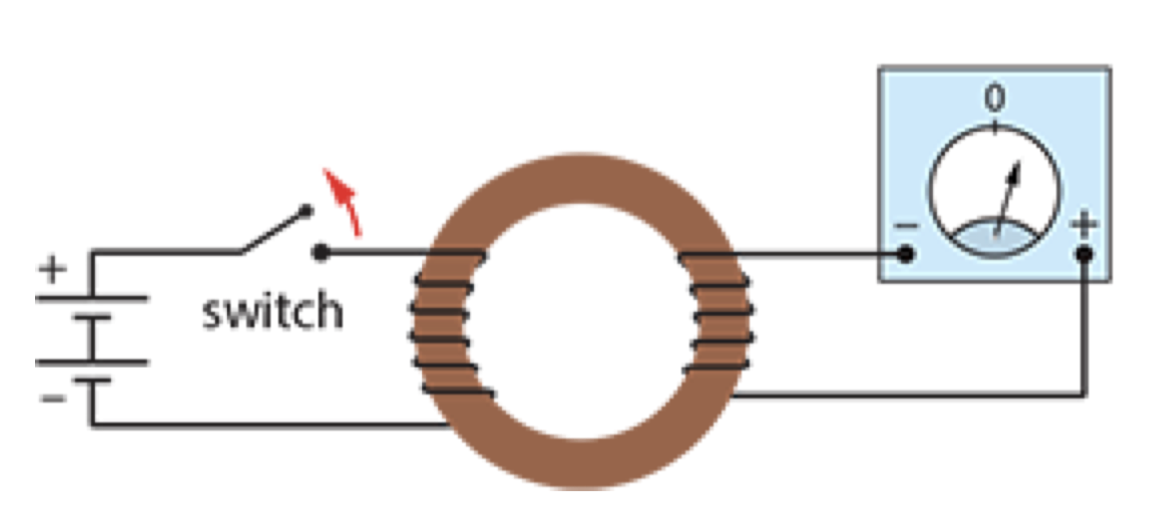
\includegraphics[width=0.5\linewidth]{Screenshot 2026-07-09 at 11.18.41.png}
\begin{circuitikz}[>=Stealth, scale=1]

  % --- Color Definitions ---
  \definecolor{coilbrown}{RGB}{165, 115, 85}   % Copper/brown color for the coil wires
  \definecolor{magnetred}{RGB}{220, 60, 50}    % Vivid red for the North pole
  \definecolor{magnetgray}{RGB}{230, 230, 230}  % Light gray for the South pole

  % --- 1. TOP BACKGROUND WIRE ---
  % Connects from the top turn of the coil to the left terminal of the galvanometer
  \draw[coilbrown, thick] (-0.6, -0.3) -- (2.8, -0.3);

  % --- 2. COIL BACK SEGMENTS (Behind the Axis/Magnet) ---
  \foreach \start/\end in {360/540, 720/900, 1080/1260, 1440/1620} {
    \draw[coilbrown, thick, smooth, samples=30] 
      plot[domain=\start:\end] ({0.6*cos(\x)}, {-0.6*\x/360 + 0.15*sin(\x)});
  }

  % --- 3. BAR MAGNET ---
  % South Pole (Top)
  \draw[fill=magnetgray, draw=black!60, thick] (-0.25, 0.6) rectangle (0.25, 1.7);
  \node[font=\bfseries, color=black!80] at (0, 1.15) {S};
  
  % North Pole (Bottom)
  \draw[fill=magnetred, draw=black!60, thick] (-0.25, -0.5) rectangle (0.25, 0.6);
  \node[white, font=\bfseries] at (0, 0.05) {N};

  % --- 4. COIL FRONT SEGMENTS (In Front of the Axis/Magnet) ---
  \foreach \start/\end in {180/360, 540/720, 900/1080, 1260/1440} {
    \draw[coilbrown, ultra thick, smooth, samples=30] 
      plot[domain=\start:\end] ({0.6*cos(\x)}, {-0.6*\x/360 + 0.15*sin(\x)});
  }

  % --- 5. BOTTOM WIRE ---
  % Routes from the bottom-left coil exit, down and around to the right terminal
  \draw[coilbrown, thick] (-0.6, -2.7) -- (-0.6, -3.2) -- (4.2, -3.2) -- (4.2, -0.3);

  % --- 6. CUSTOM DETAILED GALVANOMETER ---
  % Outer Casing
  \draw[thick, fill=gray!15, rounded corners=4pt] (2.8, -1.1) rectangle (4.2, 0.6);
  
  % Inner Display Window
  \draw[thick, fill=white] (2.9, -0.4) -- (2.9, 0.1) arc(180:0:0.6) -- (4.1, -0.4) -- cycle;
  
  % Measurement Scale Arc
  \draw[thick] (3.1, 0.1) arc (145:35:0.49);
  
  % Scale Ticks (Center-zero configuration)
  \foreach \a in {60, 75, 90, 105, 120} {
    \draw[thin] (3.5, -0.2) ++(\a:0.43) -- ++(\a:0.07);
  }
  \node[font=\tiny, text=black!50] at (3.5, 0.42) {0};
  
  % Deflected Indicator Needle
  \draw[red, thick, -{Stealth[scale=0.8]}] (3.5, -0.2) -- ++(70:0.52);
  \fill[black] (3.5, -0.2) circle (0.04);
  
  % Instrument Label
  \node[font=\small\bfseries, color=black!70] at (3.5, -0.85) {G};
  
  % Connection Binding Posts / Terminals
  \fill[black!80] (2.8, -0.3) circle (0.05);
  \fill[black!80] (4.2, -0.3) circle (0.05);

  % Polarity Signs
  \node[above left=0.05cm, font=\bfseries\footnotesize] at (2.8, -0.3) {$-$};
  \node[above right=0.05cm, font=\bfseries\footnotesize] at (4.2, -0.3) {$+$};

  % --- 7. MOTION INDICATOR ARROWS ---
  \draw[red, ->, thick] (-1.2, 0.5) -- (-1.2, 1.4);
  \draw[red, ->, thick] (-1.0, 1.4) -- (-1.0, 0.5);

\end{circuitikz}
\end{center}
The current is created as a result of the motion of the magnet relative to the coil. The current registered by the galvanometer increases when:
\begin{itemize}
  \item the relative speed of the magnet and the coil increases
  \item the strength of the magnet increases
  \item the number of turns increases
  \item the area of the loop increases
  \item the magnet moves at right angles to the plane of the loop.
\end{itemize}
The magnetic flux through the loop of wire is given as $\Phi=BA\cos\theta$, where $B$ is the magnetic flux density, $A$ is the area of the loop and $\theta$ is the angle between the normal to the plane of the loop and the direction of the magnetic field.
\begin{center}
  \begin{tikzpicture}[>=Stealth, scale=1]

  % Rotated Flux Collecting Elliptical Surface Loop
  \definecolor{looporange}{RGB}{230, 150, 80}
  \draw[fill=looporange!60, draw=looporange!90!black, thick, rotate=-22] (0,0) ellipse (1.2 and 0.45);
  \node[below] at (0, -0.6) {area $A$};
  
  % Uniform Vector Fields B (Vertical Axis Alignment)
  \draw[green!60!black, ->, ultra thick] (0,0) -- (0, 2.2) node[above, black] {$B$};
  \node[left, text width=2.2cm, align=right, font=\small] at (-0.2, 1.5) {direction of\\magnetic field};
  
  % Perpendicular Vector (Surface Normal Line)
  \draw[black, ->, thick] (0,0) -- (48:2.0) node[right, text width=1.8cm, font=\small] {normal to\\loop};
  
  % Angular Coordinate Arc Intersection
  \draw[thick] (0, 0.7) arc (90:48:0.7);
  \node[above right] at (68:0.65) {$\theta$};

\end{tikzpicture}
\end{center}
The magnetic flux multiplied by the number of turns in a loop is called the flux linkage, $\Phi=NBA\cos\theta$.\\
The intuitive picture of magnetic flux is the number of magnetic field lines that pierce the loop area. 
\begin{center}
\begin{tikzpicture}[>=Stealth, scale=1]

  % --- Color Definitions ---
  \definecolor{loopbrown}{RGB}{175, 110, 50}    % Warm brown for the wire loops
  \definecolor{fieldgreen}{RGB}{125, 185, 85}   % Vibrant green for magnetic field lines
  \definecolor{normalbrown}{RGB}{140, 90, 40}   % Darker brown for the normal vector

  % =========================================================================
  % PANEL A: Field Parallel to Loop Plane (Zero Flux)
  % =========================================================================
  \begin{scope}[shift={(0,0)}]
    \node[below, font=\small] at (0, -1.2) {$\Phi=0$};
    % Magnetic Field Lines (Horizontal arrows)
    \foreach \y in {0.5, 0, -0.5} {
      \draw[fieldgreen, ->, ultra thick] (-1.8, \y) -- (1.8, \y);
    }
    
    % Wire Loop (Rectangle)
    \draw[loopbrown, ultra thick] (-1.2, -0.9) rectangle (1.2, 0.9);
  \end{scope}


  % =========================================================================
  % PANEL B: Field Perpendicular to Loop Plane (Maximum Flux)
  % =========================================================================
  \begin{scope}[shift={(4.5,0)}]
    
    % Wire Loop (Rectangle)
    \draw[loopbrown, ultra thick] (-1.2, -0.9) rectangle (1.2, 0.9);
    \node[below, font=\small] at (0, -1.2) {$\Phi_\text{max}$};
    % Into-the-Page Magnetic Field Grid (\otimes symbols)
    \foreach \x in {-0.8, -0.2, 0.4, 0.8} {
      \foreach \y in {0.5, 0, -0.5} {
        \draw[fieldgreen, thick] (\x, \y) circle (0.11);
        \draw[fieldgreen, thick] (\x-0.07, \y-0.07) -- (\x+0.07, \y+0.07);
        \draw[fieldgreen, thick] (\x-0.07, \y+0.07) -- (\x+0.07, \y-0.07);
      }
    }
  \end{scope}


  % =========================================================================
  % PANEL C: Field at an Angle to Loop Normal (General Flux)
  % =========================================================================
  \begin{scope}[shift={(9.0,0)}]
    
    % Background/Passing Magnetic Field Lines
    \foreach \y in {0.7, 0.35, -0.35, -0.7} {
      \draw[fieldgreen, ->, ultra thick] (-1.8, \y) -- (1.8, \y);
    }
    
    % Tilted Wire Loop (Parallelogram to simulate 3D rotation)
    % Center is at (0,0)
    \coordinate (Top) at (0.15, 1.2);
    \coordinate (Right) at (0.95, -0.2);
    \coordinate (Bottom) at (-0.15, -1.2);
    \coordinate (Left) at (-0.95, 0.2);
    \draw[loopbrown, ultra thick] (Top) -- (Right) -- (Bottom) -- (Left) -- cycle;
    
    % Central Field Line pointing exactly through origin for angle definition
    \draw[fieldgreen, ->, ultra thick] (-1.8, 0) -- (1.8, 0);
    
    % Surface Normal Vector (Perpendicular to the tilted plane)
    \draw[normalbrown, ->, ultra thick] (0, 0) -- (32:1.4);
    
    % Angle Theta Arc & Label
    \draw[thick] (0.45, 0) arc (0:32:0.45);
    \node[font=\small] at (16:0.65) {$\theta$};
  \end{scope}

\end{tikzpicture}
\end{center}
\subsubsection*{Faraday's Law}
The current generated by a magnetic field is correlated with the rate of change of magnetic flux linkage through the loop. Changing flux creates an induced $e.m.f$, not necessarily a current. There will only be a current if the loop is conducting; that is, if the resistance of the circuit is not infinite.
The induced $e.m.f$ is equal to the (negative) rate of change of magnetic flux linkage:
\[\varepsilon=-N\dfrac{\Delta \Phi}{\Delta t}\left(=-N\dfrac{\mathrm{d}\Phi}{\mathrm{d}t}\right)\]
\subsubsection*{Lenz's Law}
It states that the direction of the induced current is such that it opposes the change in magnetic flux that produced it. This is a consequence of the conservation of energy and is reflected in the negative sign in Faraday's Law.
\begin{itemize}
  \item If the flux increases, the induced $e.m.f$ will create a current whose magnetic field is opposite to the external field. 
  \item If the flux decreases, the induced $e.m.f$ will create a current whose magnetic field is parallel to the external field.
\end{itemize}
\begin{center}
  \begin{tikzpicture}[scale=0.9]
    % Define custom styles for magnetic field vectors
    \tikzset{
        green_cross/.pic={
            \draw[green!60!black, thick] (0,0) circle (0.13);
            \draw[green!60!black, thick] (-0.08,-0.08) -- (0.08,0.08);
            \draw[green!60!black, thick] (-0.08,0.08) -- (0.08,-0.08);
        },
        blue_cross/.pic={
            \draw[blue!70!cyan, thick] (0,0) circle (0.11);
            \draw[blue!70!cyan, thick] (-0.07,-0.07) -- (0.07,0.07);
            \draw[blue!70!cyan, thick] (-0.07,0.07) -- (0.07,-0.07);
        },
        blue_dot/.pic={
            \draw[blue!70!cyan, thick] (0,0) circle (0.11);
            \fill[blue!70!cyan] (0,0) circle (0.03);
        }
    }

    % Background Green Magnetic Field Grid
    \foreach \x in {1.0, 1.8, 2.6, 3.4, 5.9, 6.7, 7.5, 8.3} {
        \pic at (\x, 3.5) {green_cross};
        \pic at (\x, -0.5) {green_cross};
    }
    \foreach \y in {0.4, 1.1, 1.9, 2.6} {
        \foreach \x in {1.0, 1.8, 2.6, 3.4, 5.9, 6.7, 7.5, 8.3} {
            \pic at (\x, \y) {green_cross};
        }
    }

    % Localized Induced Blue Magnetic Field
    \foreach \y in {0.8, 1.5, 2.2} {
        \pic at (4.1, \y) {blue_dot};
        \pic at (5.4, \y) {blue_cross};
    }

    % Conducting Rails & Left Connection Wire
    \draw[black, very thick] (0.5, 3) -- (8.8, 3);
    \draw[black, very thick] (0.5, 0) -- (8.8, 0);
    \draw[black, very thick] (0.5, 0) -- (0.5, 3);

    % Resistor R
    \filldraw[fill=white, draw=black, thick] (0.35, 0.8) rectangle (0.65, 2.2);
    \node[left, font=\large] at (0.3, 1.5) {$R$};

    % Moving Conducting Bar
    \filldraw[fill=orange!20, draw=black, thick] (4.4, 0) rectangle (4.9, 3);
    
    % Induced Current Arrow inside the Bar
    \draw[blue!80!black, ultra thick, -{Stealth[scale=1.5]}] (4.65, 0.4) -- (4.65, 2.6);

    % Velocity Arrow
    \draw[red!85!black, ultra thick, -{Stealth[scale=1.5]}] (4.9, 1.5) -- (6.3, 1.5) node[right, black, font=\large\itshape] {v};

    % Dashed Loop Rectangle
    \draw[dashed, black, thick] (0.2, -0.2) rectangle (5.1, 3.2);

    % Length Dimension L
    \draw[{Stealth[scale=1.2]}-{Stealth[scale=1.2]}, thick] (2.9, 0) -- (2.9, 3) node[midway, fill=white, font=\large] {$L$};
\end{tikzpicture}
\begin{tikzpicture}[scale=0.6,>=Stealth]

% Colors
\definecolor{orbit}{RGB}{225,120,20}
\definecolor{bluevec}{RGB}{40,110,220}
\definecolor{greenx}{RGB}{135,190,70}

\def\r{2}

%--------------------------------------------------
% Background magnetic field (green crosses)
%--------------------------------------------------
\foreach \x in {-3,0,3}
{
    \foreach \y in {-3,0,3}
    {
        \draw[greenx, line width=1pt] (\x,\y)+(-0.09,-0.09)--+(0.09,0.09);
        \draw[greenx, line width=1pt] (\x,\y)+(-0.09,0.09)--+(0.09,-0.09);
        \draw[greenx] (\x,\y) circle (0.22);
    }
}

\foreach \x in {-3,3}
{
    \foreach \y in {-1.5,1.5}
    {
        \draw[greenx, line width=1pt] (\x,\y)+(-0.09,-0.09)--+(0.09,0.09);
        \draw[greenx, line width=1pt] (\x,\y)+(-0.09,0.09)--+(0.09,-0.09);
        \draw[greenx] (\x,\y) circle (0.22);
    }
}

\foreach \y in {-1.5,1.5}
{
    \draw[greenx, line width=1pt] (0,\y)+(-0.09,-0.09)--+(0.09,0.09);
    \draw[greenx, line width=1pt] (0,\y)+(-0.09,0.09)--+(0.09,-0.09);
    \draw[greenx] (0,\y) circle (0.22);
}

%--------------------------------------------------
% Straight wire
%--------------------------------------------------
\draw[line width=2pt,orange!80] (-4,-3.2)--(-4,3.2);
\draw[green!70!black, line width=2pt,-Stealth] (-4,-1)--(-4,1);

%--------------------------------------------------
% Circular path
%--------------------------------------------------
\draw[orbit,line width=1.6pt] (0,0) circle (\r);

%--------------------------------------------------
% Direction arrows on orbit
%--------------------------------------------------
\draw[bluevec,line width=2pt,-Stealth]
    (-2,0.15) arc (176:135:\r);

\draw[bluevec,line width=2pt,-Stealth]
    (-0.2,2) arc (96:40:\r);

\draw[bluevec,line width=2pt,-Stealth]
    (2,-0.15) arc (-4:-45:\r);

\draw[bluevec,line width=2pt,-Stealth]
    (0.2,-2) arc (-84:-140:\r);

%--------------------------------------------------
% Blue magnetic field symbols around the loop
%--------------------------------------------------

% Top
\draw[blue,line width=1pt] (0,2.55) circle (0.18);
\fill[blue] (0,2.55) circle (0.04);

\draw[blue,line width=1pt] (0,1.75) circle (0.18);
\draw[blue,line width=1pt] (0,1.75)+(-0.08,-0.08)--+(0.08,0.08);
\draw[blue,line width=1pt] (0,1.75)+(-0.08,0.08)--+(0.08,-0.08);

% Left
\draw[blue,line width=1pt] (-2.55,0) circle (0.18);
\fill[blue] (-2.55,0) circle (0.04);

\draw[blue,line width=1pt] (-1.75,0) circle (0.18);
\draw[blue,line width=1pt] (-1.75,0)+(-0.08,-0.08)--+(0.08,0.08);
\draw[blue,line width=1pt] (-1.75,0)+(-0.08,0.08)--+(0.08,-0.08);

% Right
\draw[blue,line width=1pt] (2.55,0) circle (0.18);
\fill[blue] (2.55,0) circle (0.04);

\draw[blue,line width=1pt] (1.75,0) circle (0.18);
\draw[blue,line width=1pt] (1.75,0)+(-0.08,-0.08)--+(0.08,0.08);
\draw[blue,line width=1pt] (1.75,0)+(-0.08,0.08)--+(0.08,-0.08);

% Bottom
\draw[blue,line width=1pt] (0,-2.55) circle (0.18);
\fill[blue] (0,-2.55) circle (0.04);

\draw[blue,line width=1pt] (0,-1.75) circle (0.18);
\draw[blue,line width=1pt] (0,-1.75)+(-0.08,-0.08)--+(0.08,0.08);
\draw[blue,line width=1pt] (0,-1.75)+(-0.08,0.08)--+(0.08,-0.08);

\end{tikzpicture}
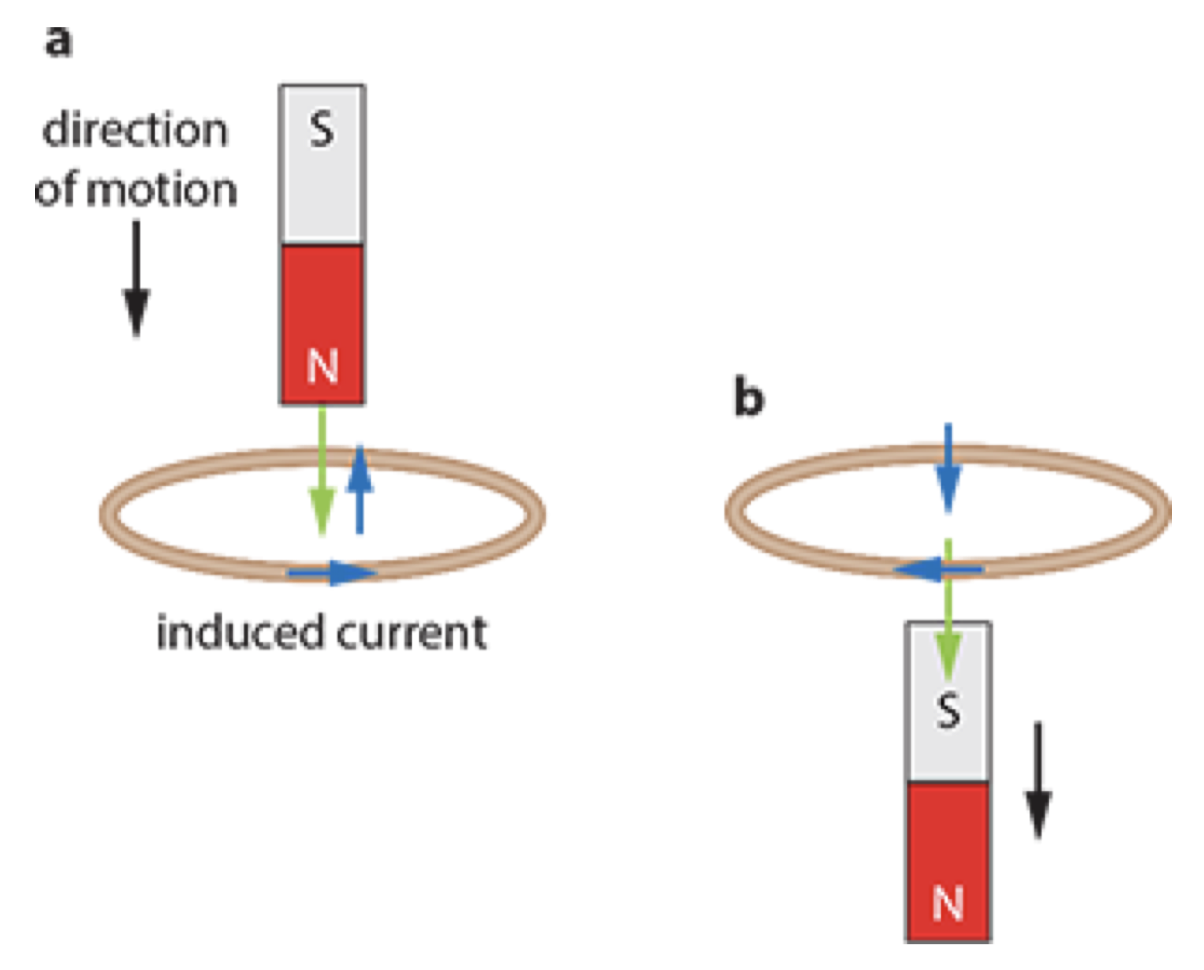
\includegraphics[width=0.25\linewidth]{Screenshot 2026-07-09 at 14.52.48.png}
\end{center}
\begin{itemize}
  \item The rod is made to move to the right. The magnetic flux through the loop is increasing and a current will be established in the rod. By Lenz's law, the current must produce a magnetic field opposite to the existing magnetic field, i.e. out of the page. (Opposing the increase of the magnetic flux $\Rightarrow$ decrease the magnetic flux, and one way is to set up a magnetic field inside the loop of the opposite direction) So the current must be counterclockwise.
  \item A loop of wire near a straight wire in which the current is decreasing. The current in the straight wire creates a magnetic field into the page at the position of the loop. The induced current in the loop produces a magnetic field in the same direction as to oppose the change in flux. From the right-hand rule, the current must be clockwise.
  \item The flux in the loop is increasing because the magnetic field at the loop is getting larger as the magnet approaches. The induced current must then oppose the increase in the flux. This can be done if the induced current produces a magnetic field in the opposite direction to that of the bar magnet. Thus, the current will flow in a counterclockwise direction when looked at from above.
\end{itemize}
\subsubsection*{Self induction}
By changing the resistance of R the current in the circuit will be changing; the magnetic flux linkage in the coil will therefore also be changing and an $e.m.f$ $\varepsilon_L$ will be induced in the coil. By Lenz's law, the induced $e.m.f$ will oppose the change in the current. The polarity of the induced $e.m.f$ is such as to drive current in the opposite direction to that of the current from the cell. In this way the induced $e.m.f$ opposes the increase in the current by decreasing the current in the circuit.
\begin{center}
  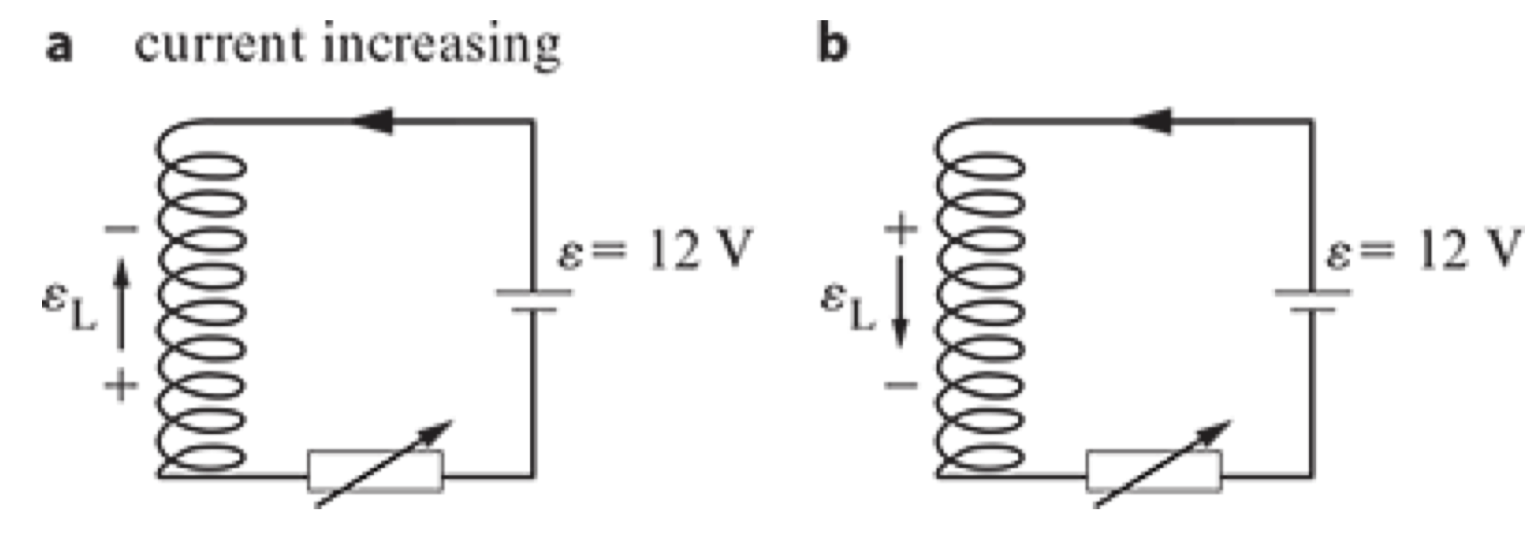
\includegraphics[width=0.4\linewidth]{Screenshot 2026-07-09 at 15.05.35.png}
\end{center}
\subsection{Generators and alternating current}
\subsubsection*{AC Generator}
A coil is made to rotate in a region of magnetic field. The ends of the coil are firmly attached to two slip rings that rotate along with the coil. The slip rings touch carbon brushes that transfer the current into an external circuit.
\begin{center}
  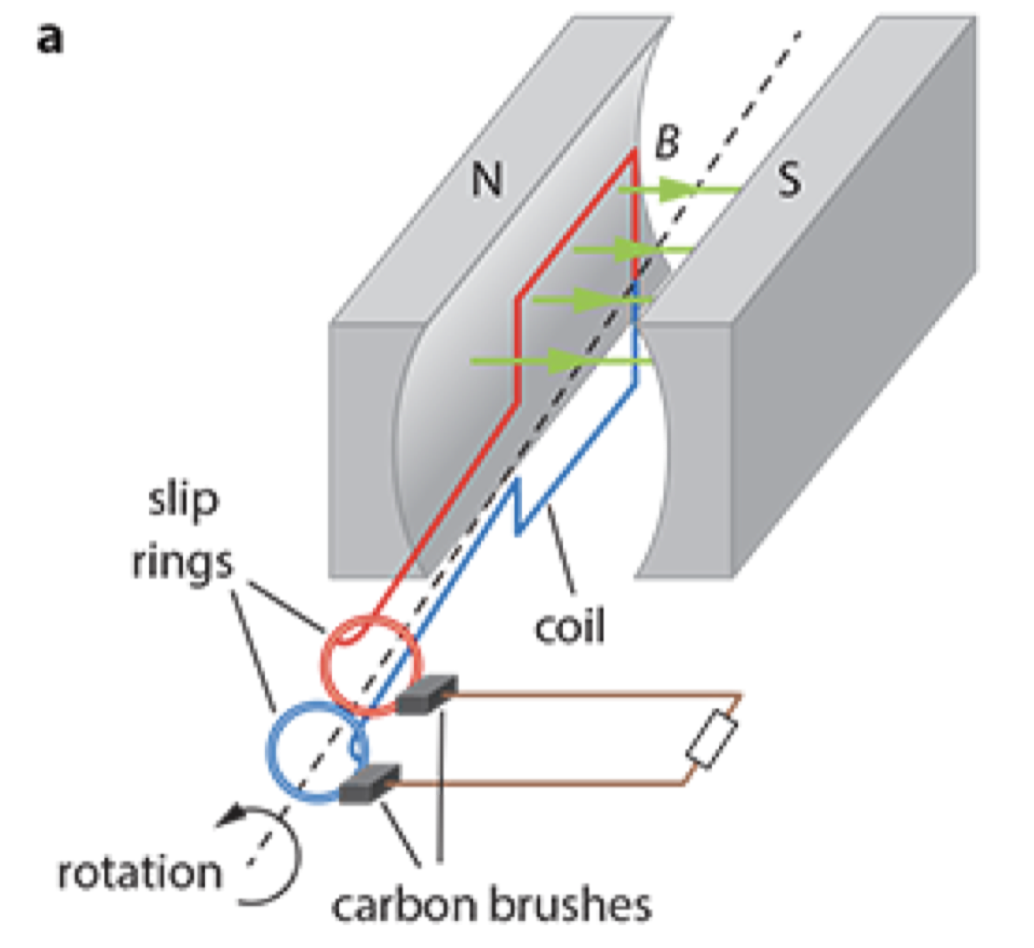
\includegraphics[width=0.3\linewidth]{Screenshot 2026-07-09 at 15.12.31.png}\\
  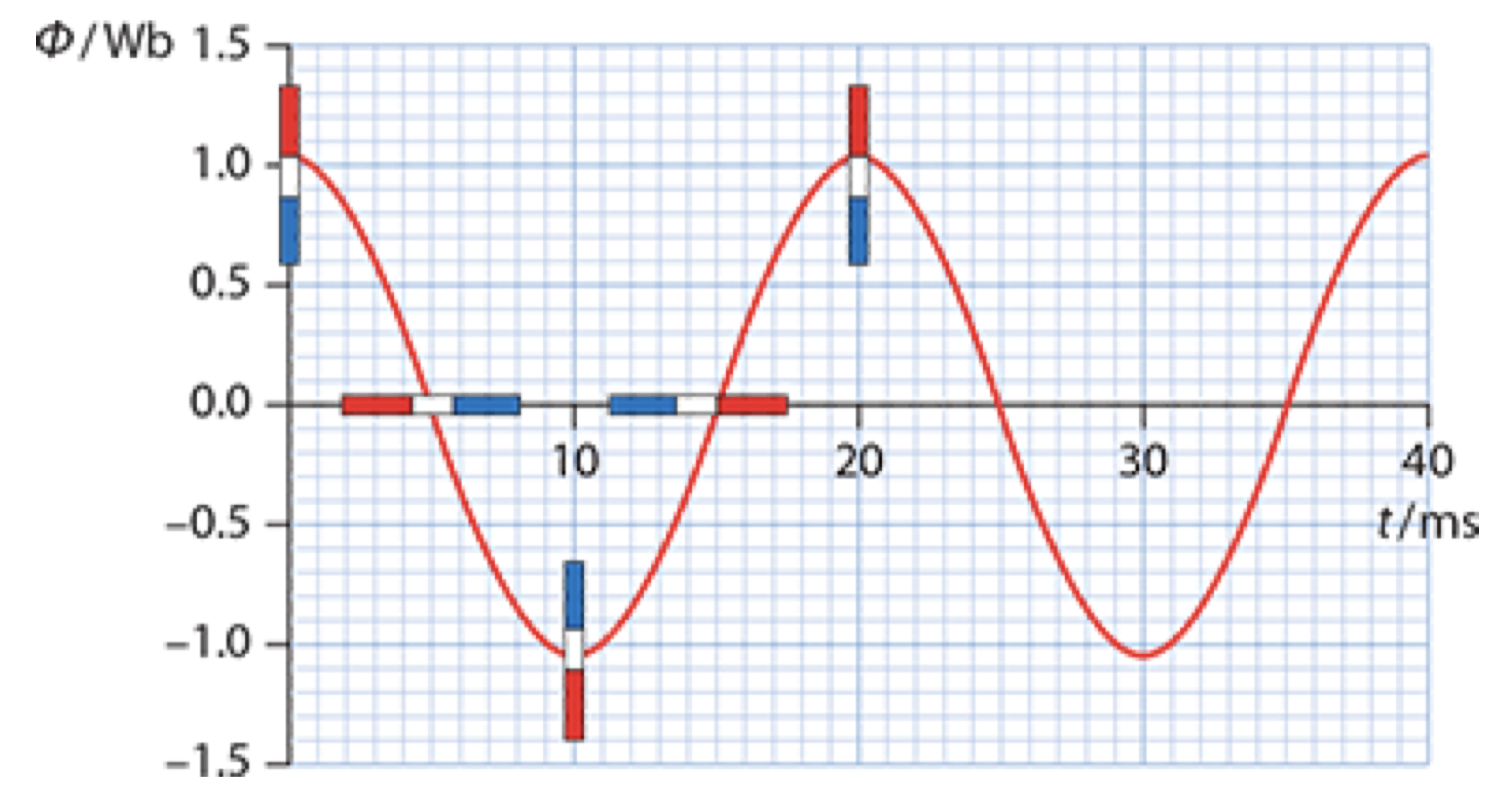
\includegraphics[width=0.4\linewidth]{Screenshot 2026-07-09 at 15.23.44.png}
  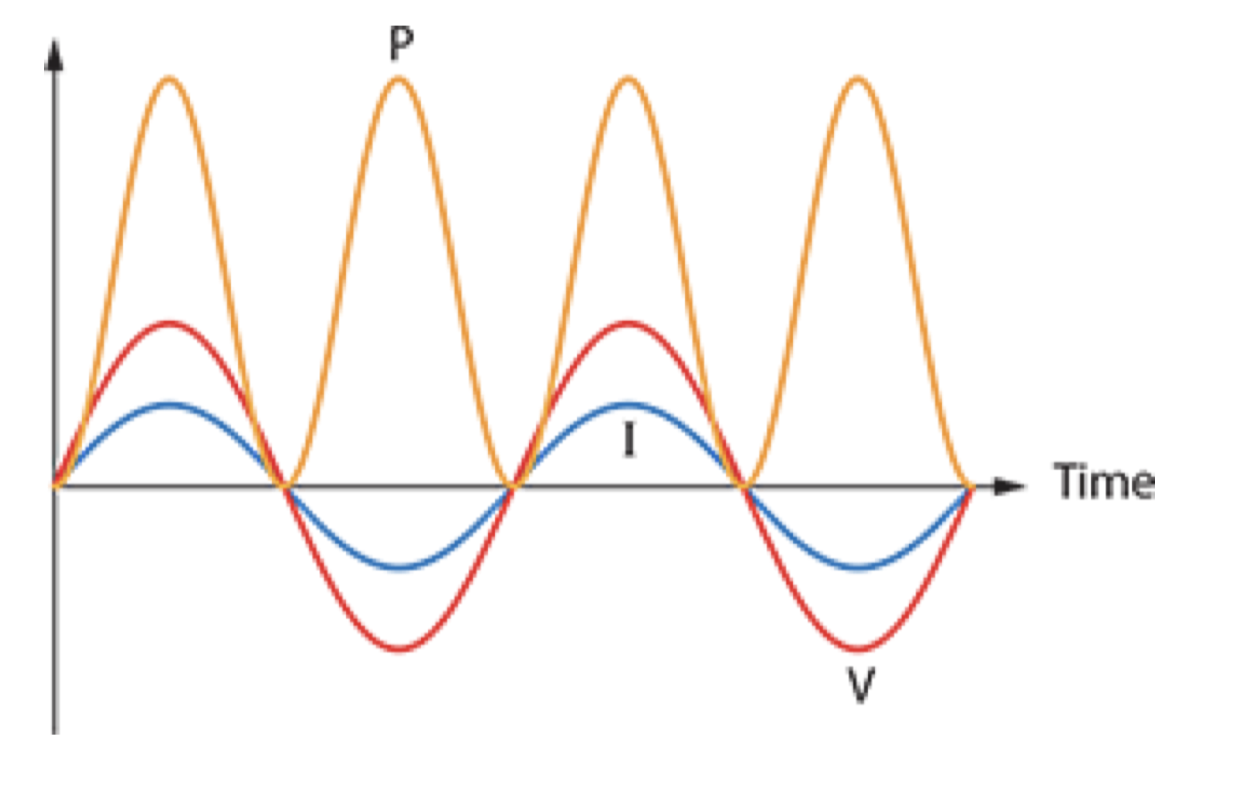
\includegraphics[width=0.32\linewidth]{Screenshot 2026-07-09 at 15.25.36.png}
\end{center}
The flux linkage in the coil changes as time goes on according to a cosine function. The red, white and blue bar that is superposed on the graph indicates the position of the coil as we look at it along the axis of rotation.
$\theta$ is the angle between the magnetic field and the normal to the coil. The coil rotates with angular speed of rotation, $\therefore \theta=\omega t=2\pi ft\Rightarrow \Phi=NBA\cos(2\pi ft)$. ($f=$ revolutions per second).
The $e.m.f$ induced is thus $V=-\dfrac{d\Phi}{dt}=2\pi fNBA\cos(2\pi ft)$. $V_\text{max}=2\pi fNBA$ when magnetic flux=0, $V_\text{min}=0$ when the magnetic flux is at its maximum / minimum. \\\\
For alternating voltage and alternating current, the electrons oscillate back and forth with the same frequency as that of the voltage. The flux and the $e.m.f$ are out of phase by $90^\circ / \dfrac{\pi}{2}$. The current is in phase with the $e.m.f$, which can be given by $I=I_\text{max}\sin(2\pi ft)=\dfrac{V_\text{max}}{R}\sin(2\pi ft)$, where the resistance $R$ is given in the circuit.
\subsubsection*{Power in AC circuits}
$$\begin{aligned}P&=V_\text{max}I_\text{max}\sin^2(2\pi ft)\\P_\text{max}&=V_\text{max}I_\text{max}\end{aligned}$$
The average power dissipated is half the peak value. Key conclusion: $V\propto f, I\propto f, P\propto f^2$.
\newpage
% ===================== Unit E =====================
\unnumberedsection{Unit E Nuclear and quantum physics}

\section{Atomic physics}
\subsection{The structure of the atom}
$\alpha$ particles were directed at a thin gold foil in an evacuated chamber. 你Rutherford哥哥又限时返场了。They found that:
\begin{itemize}
  \item the great majority of the alpha particles went straight through the foil with no or little deflection; they were detected at very small scattering angles: they were due to the electric force of repulsion between the positive charge of the gold atoms and the positive charge of the alpha particles. The effect of the electrons of the gold atoms on the path of the alpha particles is negligible.
  \item very occasionally, alpha particles were detected at very large scattering angles. \textbf{The repulsion force must be very large and thus the separation must be very small. This could only be explained if the positive charge on the atom is within a sphere that is much smaller than the sphere that Thomson had imagined.} This and subsequent experiments confirmed the existence of the nucleus inside the atom: a small, massive object carrying the positive charge of the atom and most of its mass.
\end{itemize}
\begin{center}
  \begin{tikzpicture}[
    >=Latex,
    scale=0.95,
    midarrow/.style={postaction={decorate, decoration={markings, mark=at position #1 with {\arrow{Latex}}}}}
]


    % Thin gold foil
    \fill[yellow!80!orange] (1.0, -1.8) rectangle (1.2, 1.8);
    \node[above] at (1.1, 1.8) {\small thin gold foil};

    % Incoming alpha particles (dashed lines with multiple arrows)
    % Path A (top)
    \draw[dashed, thick, midarrow=0.4, midarrow=0.8] (-3, 1.0) -- (1.0, 1.0);
    \draw[dashed, thick, -Latex] (1.2, 1.0) -- (4.5, 2.0) node[right] {A};

    % Path B (mid-top)
    \draw[dashed, thick, midarrow=0.4, midarrow=0.8] (-3, 0.33) -- (1.0, 0.33);
    \draw[dashed, thick, -Latex] (1.2, 0.33) -- (4.5, 0.33) node[right] {B};

    % Path C (mid-bottom)
    \draw[dashed, thick, midarrow=0.4, midarrow=0.8] (-3, -0.33) -- (1.0, -0.33);
    \draw[dashed, thick, -Latex] (1.2, -0.33) -- (4.5, -1.3) node[right] {C};

    % Path L (bottom, large angle scattering)
    \draw[dashed, thick, midarrow=0.4, midarrow=0.8] (-3, -1.0) -- (1.0, -1.0);
    \draw[dashed, thick, -Latex] (1.0, -1.0) .. controls (0.2, -1.0) and (0.5, -2.0) .. (-1.2, -2.0) node[left] {L};

    % Labels for diagram (a)
    \node[above] at (-1.5, 1.1) {\small alpha particles};
    \node[below, align=center] at (-0.5, -2.5) {\small large-angle scattering};
    \node[below, align=center] at (3.5, -2.5) {\small small-angle scattering};


    % ==========================================
    % Diagram (b)
    % ==========================================
    \begin{scope}[shift={(11,0)}]

        % Vacuum chamber outline
        \draw[thick] (0,0) circle (3);
        \node[above] at (0, 2.3) {\small vacuum};

        % Source of alpha particles (Lead block)
        % Using white fill to "cut" the circle boundary, then hatch pattern
        \fill[white] (-3.8, 0.8) rectangle (-2.0, -0.8);
        \draw[thick, pattern=north east lines, pattern color=black] 
            (-3.8, 0.8) -- (-2.0, 0.8) -- (-2.0, 0.15) -- (-3.2, 0.15) -- 
            (-3.2, -0.15) -- (-2.0, -0.15) -- (-2.0, -0.8) -- (-3.8, -0.8) -- cycle;
        
        % Small circle for the actual source
        \draw[thick, fill=white] (-3.0, 0) circle (0.1);

        % Source label
        \node[left, align=center] (src) at (-4.0, -0.5) {\small source of\\[-0.5ex]\small alpha particles};
        \draw (src.east) -- (-3.1, -0.05);

        % Alpha particle beam (red)
        \draw[thick, red, -Latex] (-2.9, 0) -- (-1.0, 0);
        \draw[thick, red] (-1.0, 0) -- (0, 0);

        % Gold foil (vertical line)
        \draw[thick, yellow!80!orange] (0, -1.5) -- (0, 1.5);
        \node[right] at (0.2, 1.2) {\small gold foil};

        % Microscope and Scattered beam (rotated scope)
        \begin{scope}[rotate=-45]
            % Scattered beam (magenta)
            \draw[thick, magenta] (0,0) -- (2.5, 0);
            
            % Microscope Tube
            \draw[thick, fill=white] (2.5, -0.3) rectangle (3.8, 0.3);
            % Front opening
            \draw[thick, fill=white] (2.5, 0) ellipse (0.1 and 0.3);
            % Back closed end
            \draw[thick, fill=white] (3.8, 0) ellipse (0.1 and 0.3); 
            
            % Spark of light (zigzag)
            \draw[thick, magenta, decorate, decoration={zigzag, segment length=1.5mm, amplitude=0.8mm}] 
                (2.8, 0) -- (3.4, 0);
        \end{scope}

        % Spark of light label
        \node[right, align=center] (spark) at (2.5, -0.8) {\small spark\\[-0.5ex]\small of light};
        \draw (spark.west) -- (2.2, -2.1);

        % Curved dashed line for microscope path
        \draw[dashed, thick, Latex-Latex] (-80:4.2) arc (-80:-10:4.2);
        \node[right] at (-45:4.4) {\small microscope};

    \end{scope}

\end{tikzpicture}
\end{center}
结论：The Rutherford experiment established the Rutherford model of the atom: the atom consists of a very small, massive, positively charged nucleus, and the electrons orbit the nucleus like planets around the sun.
\subsubsection*{Discrete energy}
If you expose a container of gas at low pressure to a strong electric field, light will be emitted from the gas. You can show that the emitted light contains many different wavelengths by passing it through a prism or diffraction grating. The result is a series of bands of light at different wavelengths. The set of possible wavelengths that can be emitted is called the emission spectrum.\\\\
Bohr argued that an atom has discrete energy, i.e. it can have one out of a specific set of values. He represented the possible energies (refers to $E_T=E_K+E_P$) with an energy level diagram. For example, the hydrogen atom in the n$^\text{th}$ state has an energy of $E=-\dfrac{13.6}{n^2}$ eV, $n\in \mathbb{Z^+}$. The negative sign in the energy tells us that the electron is trapped within the atom. To have the electron leave the atom, energy must be provided.\\
Bohr suggested that an atom can make a transition from a state of higher energy to a state of lower energy by emitting a photon. The energy of the emitted photon is the difference in energy of the two levels. \\
The energy of a photon is given by $E=hf=h\dfrac{c}{\lambda}$, where $h=6.63\times 10^{-34}\ \text{J\,s}$ is Planck's constant.\\
In a transition from a high to lower energy state, the wavelength of the emitted photon is given by $\lambda=\dfrac{hc}{\Delta E}$.\\
When undisturbed, the electron in the atom will occupy the lowest energy state, called the ground state. When energy is supplied to the atom, the electron can be excited to a higher energy state, called an excited state. From the excited state, the electron can return to the ground state by emitting photons, either going to ground state straightaway or passing through multiple transition energy levels, and the decision between the two chances is an issue of chance.
\begin{center}
  \definecolor{levelred}{RGB}{200, 50, 50}
\definecolor{photonmagenta}{RGB}{200, 50, 200}
\definecolor{electrongreen}{RGB}{50, 120, 50}

\begin{tikzpicture}[
    photon/.style={thick, photonmagenta, decorate, decoration={snake, amplitude=1.5mm, segment length=5.5mm, post length=3mm}, -{Latex[length=3mm]}},
    transition/.style={thick, black, -{Latex[length=3mm]}},
    electron/.style={circle, fill=electrongreen, draw=electrongreen!70!black, minimum size=0.7cm},
    scale=0.8
]
    % --- Left Diagram ---
    \begin{scope}[shift={(0,0)}]
        % Energy Levels
        \draw[levelred, line width=1.2pt] (0, 0) -- (6, 0);
        \draw[levelred, line width=1.2pt] (0, 2) -- (6, 2);
        \draw[levelred, line width=1.2pt] (0, 4) -- (6, 4);

        % Labels
        \node[anchor=west] at (6.1, 0) { $n = 1$};
        \node[anchor=west] at (6.1, 2) { $n = 2$};
        \node[anchor=west] at (6.1, 4) { $n = 3$};

        % Electron and Transition
        \node[electron] (e1) at (2, 4) {};
        \draw[transition] (2, 3.6) -- (2, 0); % Shifted down to start from bottom of electron

        % Photon
        \draw[photon] (2.3, 0.4) -- (5.5, 3.2); % Adjusted path to cross and end high
    \end{scope}

    % --- Right Diagram ---
    \begin{scope}[shift={(8,0)}]
        % Energy Levels
        \draw[levelred, line width=1.2pt] (0, 0) -- (6, 0);
        \draw[levelred, line width=1.2pt] (0, 2) -- (6, 2);
        \draw[levelred, line width=1.2pt] (0, 4) -- (6, 4);

        % Labels
        \node[anchor=west] at (6.1, 0) { $n = 1$};
        \node[anchor=west] at (6.1, 2) { $n = 2$};
        \node[anchor=west] at (6.1, 4) { $n = 3$};

        % Electron and Transitions
        \node[electron] (e2) at (1.5, 4) {};
        
        % First transition n=3 -> n=2
        \draw[transition] (1.5, 3.6) -- (1.5, 2.05); % Ends just above the level
        
        % Second transition n=2 -> n=1
        \draw[transition] (3.5, 1.95) -- (3.5, 0.05); % Starts just below and ends just above

        % Photons
        % First photon from n=3 -> n=2 cascade
        \draw[photon] (1.8, 2.3) -- (4.8, 5.0); % Starts between levels, crosses high
        
        % Second photon from n=2 -> n=1 cascade
        \draw[photon] (3.8, 0.4) -- (6.5, 2.4); % Starts lower, crosses middle
    \end{scope}

\end{tikzpicture}
\end{center} 
\subsubsection*{Absorption Spectra}
Now imagine sending a beam of white light through a gas. The majority of the atoms in the gas are in their ground state. Electrons in the atoms may absorb photons in the beam and move to an excited state. This will happen only if the photon that is to be absorbed has exactly the right energy.
This means that the light that is transmitted through the gas will be missing the photons that have been absorbed. This gives rise to absorption spectra.\\
Note: Why are the photons missing? This is because the photons are emitted in all directions and not necessarily along the direction the observer is looking.
\begin{center}
  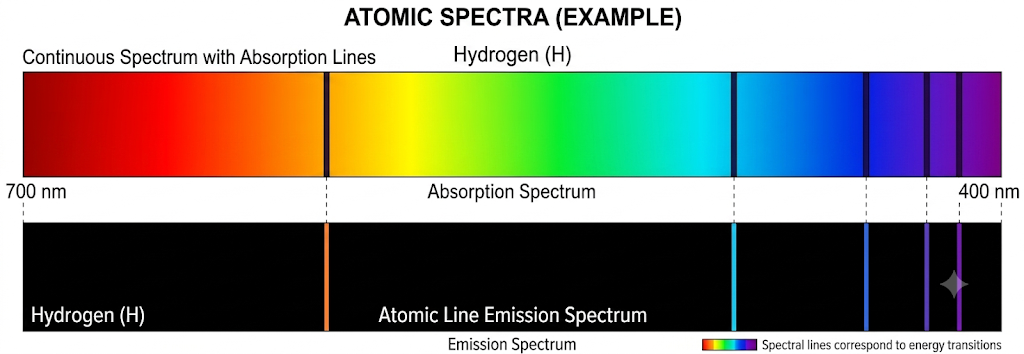
\includegraphics[width=0.7\linewidth]{Pasted 2026-07-09 at 16.44.09.png}
\end{center}
Experiments show that no two elements have the same wavelengths in their emission and absorption spectra.
\subsection{Quantisation of angular momentum}
Bohr assumed that the electron could only exist in certain special orbits satisfying the condition $$mvr=n\dfrac{h}{2\pi},\ n\in\mathbb{Z^+}$$
where $L=mvr$, angular momentum of the electron, is quantised. The electron can only occupy orbits for which the angular momentum is an integer multiple of $\dfrac{h}{2\pi}$. \\\\
The total energy $E_T$ of the orbiting electron is
\[E_T=\underbrace{\dfrac{1}{2}mv^2}_{E_K}+\underbrace{\left(-k\dfrac{e^2}{r}\right)}_{E_P}\]
The electron is acted upon the electric force, therefore
\[\begin{aligned}\dfrac{ke^2}{r^2}&=\dfrac{mv^2}{r}\\\dfrac{ke^2}{r}&=mv^2\end{aligned}\]
\[\begin{aligned}
E_T&=\dfrac{1}{2}\dfrac{ke^2}{r}-\dfrac{ke^2}{r}\\&=-\dfrac{1}{2}\dfrac{ke^2}{r}\\&=-\dfrac{1}{2}\dfrac{ke^2}{a_0}\times\dfrac{1}{n^2}
\end{aligned}\]
Squaring the quantisation of angular momentum equation gives
\[\begin{aligned}m^2v^2r^2&=n^2\dfrac{h^2}{4\pi^2}\\mv^2&=n^2\dfrac{h^2}{4\pi^2r^2}\\\dfrac{ke^2}{r}&=n^2\dfrac{h^2}{4\pi^2r^2}\\r&=a_0n^2\\&=\dfrac{n^2h^2}{4\pi^2ke^2m},\ n\in\mathbb{Z^+}\end{aligned}\]
Therefore the orbital radius can't be arbitrary, but must be one of the discrete values given by the above equation. 
The Bohr radius is the smallest possible orbital radius, given by $$a_0=\dfrac{h^2}{4\pi^2ke^2m}\approx5.29\times 10^{-11}\text{ m}$$
\section{Quantum physics}
\subsection{Photons and the photoelectric effect}
\subsubsection*{Photons}
Einstein suggested that light should be thought of as a collection of quanta, or bundles of energy. Each quantum or bundle of light has energy $E=hf$, where $f$ is the frequency of light. 
A beam of light is now to be thought of as a very large number of these quanta moving at the speed of light. The total energy of the beam is then $Nhf$, where $N$ is the number of quanta in the beam.
The energy of the beam is therefore an integral multiple of the basic unit $hf$. The photon is a particle with zero mass and zero electric charge.\\\\
In Einstein's theory of special relativity the total energy $E$, the momentum $p$ and the mass $m$ of a particle are related according to $E^2=(pc)^2+(mc^2)^2=p^2c^2+m^2c^4$. Therefore the photon has a momentum of $p=\dfrac{E}{c}=\dfrac{hf}{c}=\dfrac{h}{\lambda}$. 
\subsubsection*{Photoelectric effect}
The photoelectric effect is the phenomenon in which light (or other forms of electromagnetic radiation) incident on a metallic surface causes electrons to be emitted from the surface.
\begin{center}
  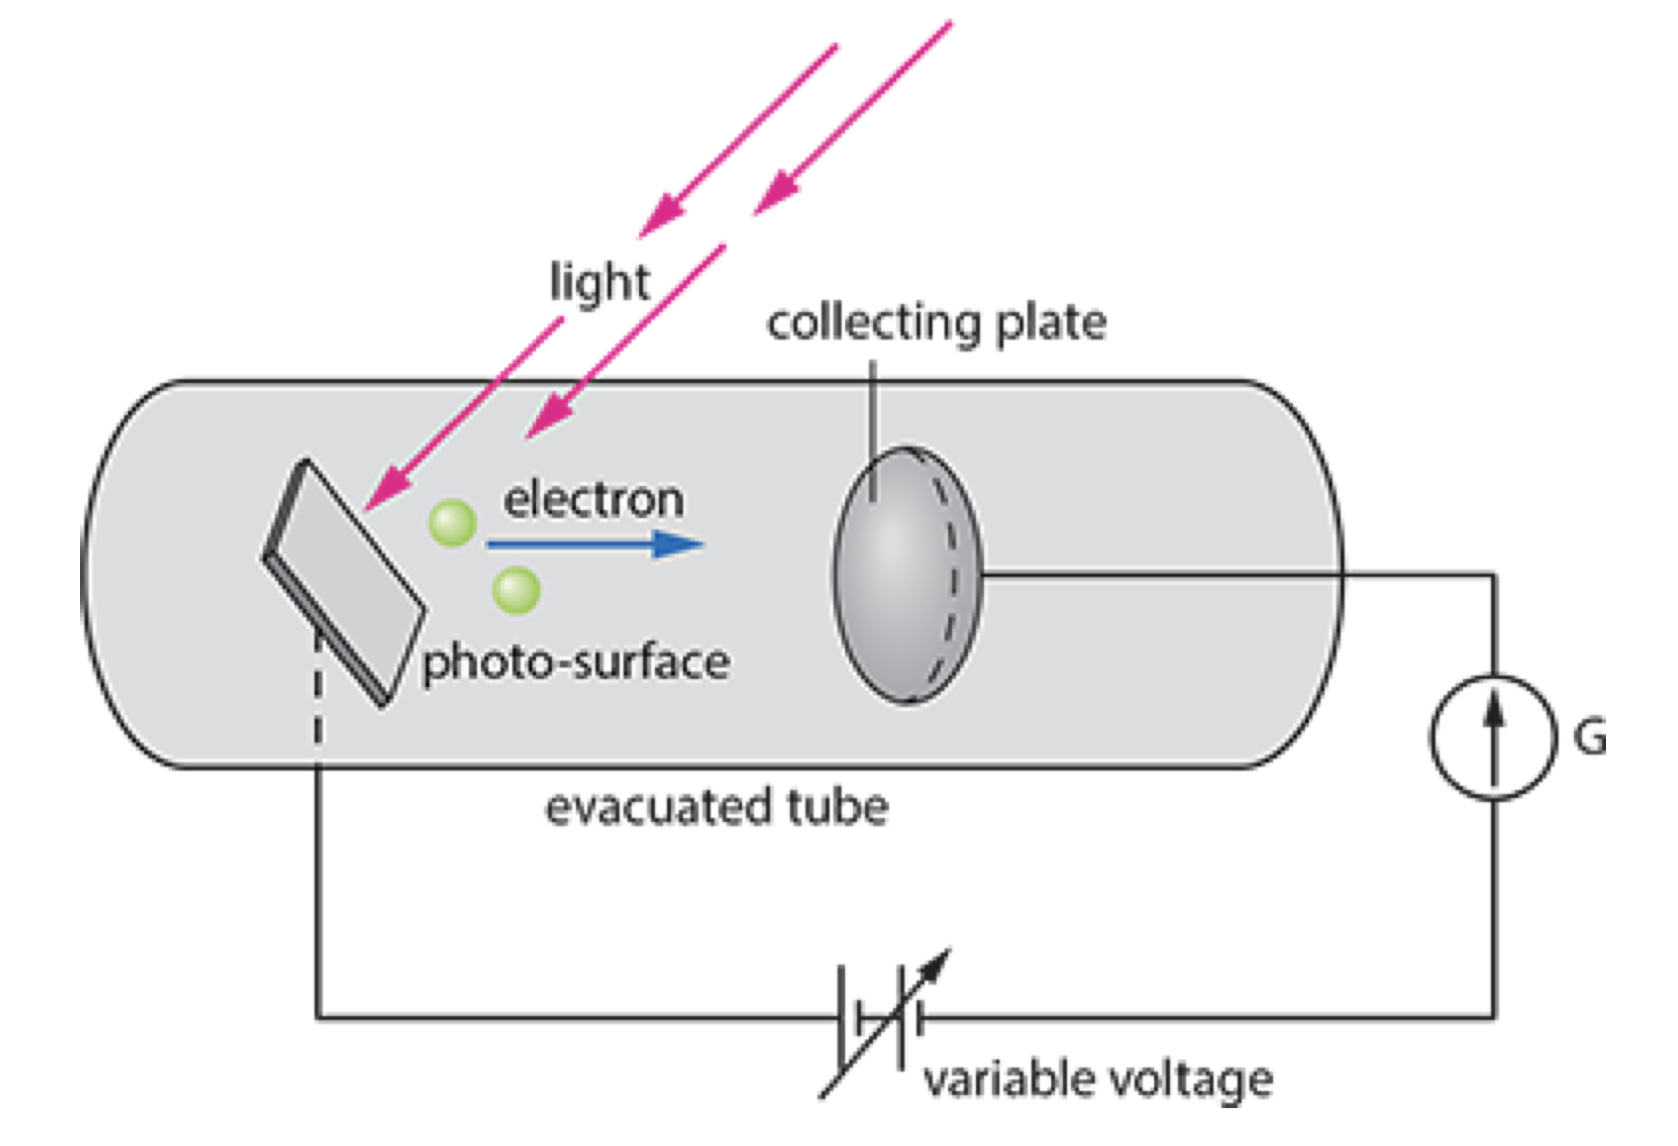
\includegraphics[width=0.5\linewidth]{Screenshot 2026-07-09 at 17.37.30.png}
\end{center}
The emitted electrons are called photoelectrons. Those electrons that make it to the collecting plate complete the circuit and so we have an electric current that is recorded by the sensitive galvanometer.
\begin{itemize}
\item Note that the terminal of the variable power supply connected to the collecting plate is the negative terminal. This means that the collecting plate actually repels the emitted electrons. Only the very energetic electrons will make it to the plate. As the magnitude of the voltage is increased (i.e. made more negative) fewer and fewer electrons make it to the plate; eventually no electron will arrive there and at that point the current becomes zero. The voltage at which the current becomes zero is called the stopping voltage $V_s$, which constitutes the formula for maximum kinetic energy for emitted photons, $E_\text{max}=eV_s$.
\item Now the positive terminal is connected to the collecting plate. The electrons are now attracted to the collecting plate and the current increases. As the voltage is increased even more the current saturates, i.e. it approaches a constant value. This is because the collecting plate is so positive that it attracts every single emitted electron.
\end{itemize}
\begin{center}
  \begin{tikzpicture}[x=1.5cm, y=2cm]

    % Grid setup
    % Voltage: -1.2 to 4.2 with sub-divisions
    % Current: -0.2 to 2.4 with sub-divisions
    \draw[cyan!30, ultra thin, step=0.1] (-1.2,-0.1) grid (4.2,2.3);
    \draw[cyan!60, thin, step=0.5] (-1.2,-0.1) grid (4.2,2.3);

    % X-Axis (Voltage)
    \draw[thick, ->, >=stealth] (-1.2,0) -- (4.3,0) node[below left, yshift=-15pt, black] {Voltage\,/\,V};
    
    % Y-Axis (Current)
    \draw[thick, ->, >=stealth] (0,-0.1) -- (0,2.4) node[above, black] {Current\,/\,nA};

    % X-Axis Ticks & Labels
    \foreach \x in {-1, 0, 1, 2, 3, 4} {
        \draw[thick] (\x, 0) -- (\x, -0.05) node[below, yshift=-2pt, black] {\small $\x$};
    }

    % Y-Axis Ticks & Labels
    \foreach \y in {0.5, 1.0, 1.5, 2.0} {
        \draw[thick] (0, \y) -- (-0.05, \y) node[left, xshift=-2pt, black] {\small $\y$};
    }

    % The Curve
    % Starts flat from -1.2 to -0.4 at Current = 0
    % Then rises sharply and curves towards saturation at (4, 2.1)
    \draw[red, very thick, line cap=round] 
        (-1.2,0) -- (-0.4,0) 
        .. controls (0.2,0.9) and (0.6,1.6) .. (1.2,1.85)
        .. controls (2.0,2.05) and (3.0,2.1) .. (4.0,2.12);

    % Annotation Arrow and Text
    \draw[thick, <-, >=stealth] (-0.4, -0.05) -- (-0.4, -0.4) 
        node[below, align=left, black, yshift=-2pt] {the stopping voltage is this\\number taken as positive};

\end{tikzpicture}
\begin{tikzpicture}[x=1.2cm, y=1.2cm, >=stealth]

    % Axes
    % Horizontal axis (frequency f)
    \draw[thick, ->] (-0.6, 0) -- (4.5, 0) node[below left, yshift=-2pt] {$f$};
    
    % Vertical axis (Kinetic Energy E_K)
    \draw[thick, ->] (0, -2.2) -- (0, 3.2) node[below left, xshift=-2pt] {$E_{\text{K}}$};

    % Origin label (0)
    \node[left, xshift=-1pt,yshift=2pt] at (0, 0) {$0$};

    % Important Coordinates
    \coordinate (phi) at (0, -1.6);     % y-intercept (-phi)
    \coordinate (fc) at (1.3, 0);       % x-intercept (threshold frequency f_c)
    \coordinate (end) at (4.0, 3.0);    % End of the solid line

    % Dashed line representing the extrapolation to the y-axis
    \draw[red!80!black, thick, dashed] (phi) -- (fc);

    % Solid line representing the physical kinetic energy values
    \draw[red!80!black, very thick] (fc) -- (end);

    % Intercept Labels
    \node[below right, xshift=2pt] at (fc) {$f_{\text{c}}$};
    \node[below right, yshift=-1pt] at (phi) {$-\phi$};

\end{tikzpicture}
\end{center}
Several conclusions were made:
\begin{enumerate}
  \item Changing the intensity of light does not affect the stopping voltage, they release electrons of the same kinetic energy.
  \item As $f$ of light increases, $E_\text{max}$ and $V_s$ increases as well.
  \item If we plot the kinetic energy of the electrons (which equals $eV_s$) versus frequency, we find a straight line. There exists a critical / threshold frequency $f_c$ such that no electrons at all are emitted if the frequency of the light source is less than $f_c$. The frequency varies with different photo-surfaces.
  \item Electrons are emitted with no time delay.
\end{enumerate}
\subsubsection*{Einstein's explanation}
A single photon of frequency $f$ is absorbed by a single electron in the photo-surface, and so the electron's energy increases by $hf$. The electron will have to spend a certain amount of energy, $\phi$ (the work function, given by $\phi=hf_c=hf-eV_s$), to free itself from the pull of the nuclei of the atoms of the photo-surface. The electron will be emitted (become free) if $hf$ is bigger than $\phi$. The difference $E_K=hf-\phi$ will be the kinetic energy of the (now) free electron.
\begin{center}
  \begin{tikzpicture}[x=1cm, y=1cm]

  % Define styles for electrons and lines
  \tikzset{
    electron bulk/.style={
      circle, minimum size=0.3cm, inner sep=0pt,
      fill=green!60, draw=green!70!black, thin
    },
    electron surface/.style={
      circle, minimum size=0.3cm, inner sep=0pt,
      fill=green!80!black, draw=black!70, thin
    },
    electron faded/.style={
      circle, minimum size=0.3cm, inner sep=0pt,
      fill=green!20, draw=black!70, dashed, thin
    },
    electron target/.style={
      circle, minimum size=0.3cm, inner sep=0pt,
      fill=green!90!black, draw=black, very thin
    },
    line style/.style={
      thick, draw=black!70
    },
    dim arrow/.style={
      <->, >=stealth, line style, thin
    }
  }

  % Define dimensions
  \def\colspacing{0.3}
  \def\rowspacing{0.3}
  \def\gridcols{6}
  \def\gridrows{7}
  \def\fadedrows{2}
  \def\wellwidth{2}
  \def\wellheight{5}
  
  \pgfmathsetmacro{\welltop}{\wellheight}
  \pgfmathsetmacro{\fadedheight}{-\fadedrows * \rowspacing}
  \pgfmathsetmacro{\surfaceY}{\gridrows * \rowspacing}

  % -- Draw Faded Bulk layers --
  \foreach \r in {1,...,\fadedrows} {
    \foreach \c in {1,...,\gridcols} {
      \pgfmathsetmacro{\xpos}{0.1 + (\c - 0.5) * \colspacing}
      \pgfmathsetmacro{\ypos}{-(\r - 0.5) * \rowspacing}
      \node[electron faded] at (\xpos, \ypos) {};
    }
  }

  % -- Draw main bulk grid of electrons --
  \foreach \r in {1,...,\gridrows} {
    \foreach \c in {1,...,\gridcols} {
      \pgfmathsetmacro{\xpos}{0.1 + (\c - 0.5) * \colspacing}
      \pgfmathsetmacro{\ypos}{(\r - 0.5) * \rowspacing}
      
      % Safe conditional drawing for the top surface row
      \pgfmathparse{\r==\gridrows ? 1 : 0}
      \ifnum\pgfmathresult=1
        \node[electron surface] at (\xpos, \ypos) {};
      \else
        \node[electron bulk] at (\xpos, \ypos) {};
      \fi
    }
  }

  % -- Pre-calculate critical coordinates to prevent parser errors --
  \pgfmathsetmacro{\ptX}{0.1 + (4 - 0.5)*\colspacing}
  \pgfmathsetmacro{\ptY}{(\gridrows - 0.5)*\rowspacing}
  \coordinate (photon_target) at (\ptX, \ptY);

  \pgfmathsetmacro{\eoX}{0.1 + (2 - 0.5)*\colspacing}
  \pgfmathsetmacro{\eoY}{(3 - 0.5)*\rowspacing}
  \coordinate (electron_origin) at (\eoX, \eoY);

  \pgfmathsetmacro{\eeX}{\wellwidth + 0.1}
  \pgfmathsetmacro{\eeY}{\welltop + 0.1}
  \coordinate (escaped_electron_pos) at (\eeX, \eeY);

  % -- Add Specific target spheres for emphasis --
  \node[electron target] at (photon_target) {};
  
  % -- Draw potential well walls --
  \draw [line style] (0, 0) -- (0, \welltop) -- (-0.5, \welltop);
  \draw [line style] (\wellwidth, 0) -- (\wellwidth, \welltop) -- (\wellwidth + 0.5, \welltop);
  
  % Dashed faded part below well
  \draw [line style, dashed, thin] (0, 0) -- (0, \fadedheight);
  \draw [line style, dashed, thin] (\wellwidth, 0) -- (\wellwidth, \fadedheight);
  \draw [line style, dashed, thin] (0, \fadedheight) -- (\wellwidth, \fadedheight);

  % energy arrow and label
  \pgfmathsetmacro{\energyArrowTop}{\welltop - 0.5}
  \draw [-{Stealth[scale=1.2]}] (-0.8, 0.5) -- (-0.8, \energyArrowTop);
  \node [left] at (-0.8, \welltop/2) {energy};

  % -- Photon wavy arrow and label --
  \pgfmathsetmacro{\photonSourceY}{\welltop + 0.9}
  \coordinate (photon_source) at (-0.6, \photonSourceY);
  \draw [pink!90!black, very thick, decorate, decoration={snake, amplitude=1.2mm, segment length=3.5mm}, -{Stealth[scale=1.2]}] (photon_source) -- (photon_target);
  \node [anchor=south west, align=left] at (photon_source.north west) {photon $hf$};

  % -- Emitted electron path and label --
  \draw [blue, -{Stealth[scale=1.2]}, thick] (electron_origin) to [out=60, in=200] (escaped_electron_pos);
  
  % Draw escaped electron and its label
  \node[electron bulk] at (escaped_electron_pos) {};
  \node [anchor=south west, align=left] at (escaped_electron_pos.east) {electron just\\escapes};

  % -- Work function (phi) arrow and label --
  \pgfmathsetmacro{\phiArrowX}{\wellwidth + 0.15}
  \pgfmathsetmacro{\phiLabelY}{(\surfaceY + \welltop)/2}
  \coordinate (phi_start) at (\phiArrowX, \surfaceY);
  \coordinate (phi_end) at (\phiArrowX, \welltop);
  
  \draw [dim arrow] (phi_start) -- (phi_end);
  \node [right] at (\phiArrowX, \phiLabelY) {$\phi$};

\end{tikzpicture}
\end{center}
We are thus able to derive this formula for stopping voltage: $V_s=\dfrac{h}{e}f-\dfrac{\phi}{e}$.
\subsubsection*{Compton scattering}
This is the scattering of light off an electron. The scattered light bounces off the electron with a longer wavelength. We can understand this in terms of photons easily: the light gives some energy to the electron which recoils with kinetic energy. The energy of the light has therefore been reduced.
\begin{center}
  \begin{tikzpicture}[>=stealth, font=\small, circle size/.style={circle, draw, minimum size=2.5mm, inner sep=0pt, outer sep=1pt}]

    % --- Axis ---
    % Define the collision point
    \coordinate (C) at (0, 0);
    % Main dashed interaction axis
    \draw[dashed, thick] (-7, 0) -- (5, 0);

    % --- Before Scattering ---
    % Define particle positions
    \coordinate (P1_pos) at (-6, 0);
    \coordinate (E1_pos) at (-3, 0);

    % Draw incident photon
    \node[circle size, fill=red!90!black, label={[align=left]above left:incident photon\\wavelength $\lambda$}] (P1) at (P1_pos) {};
    \draw[->, thick, solid] (P1.center) -- (-4.5, 0);

    % Draw electron at rest
    \node[circle size, fill=blue!90!black, label={[align=left, text width=2.2cm, xshift=0.3cm]below:electron at rest}] (E1) at (E1_pos) {};

    % General label for "before scattering"
    \node[below, text height=0.5cm] at (-6.5, -1.2) {before scattering};


    % --- After Scattering ---
    % Define the angles and positions of particles
    \def\thetaValue{35} % Scattering angle of the photon
    \def\recoilAngle{-45} % Recoil angle of the electron
    \def\photonDistance{4}
    \def\electronDistance{3.2}

    \coordinate (P2_pos) at (\thetaValue:\photonDistance);
    \coordinate (E2_pos) at (\recoilAngle:\electronDistance);

    % Draw dashed lines for paths from the collision point
    \draw[dashed, thick] (C) -- +({\thetaValue}:\photonDistance+1);
    \draw[dashed, thick] (C) -- +({\recoilAngle}:\electronDistance+1);

    % Draw scattered photon
    \node[circle size, fill=red!90!black] (P2) at (P2_pos) {};
    % Use a node for the label, precisely positioned
    \node[right=3pt, align=left] at (P2.east) {scattered photon\\wavelength $\lambda'$};
    \draw[->, thick, solid] (P2.center) -- +(\thetaValue:1);

    % Draw recoiling electron
    \node[circle size, fill=blue!90!black] (E2) at (E2_pos) {};
    % A label node placed above and to the right of the particle, multiline text
    \node[above right=10pt and 3pt, anchor=west, align=left, yshift=-3pt] at (E2.east) {recoiling\\electron};
    \draw[->, thick, solid] (E2.center) -- +(\recoilAngle:0.9);

    % Draw angle arc and label
    \draw (1.2, 0) arc (0:\thetaValue:1.2);
    \node at ({\thetaValue/2}:1.5) {$\theta$};

    % General label for "after scattering"
    % Positioned near the collision point, below the axis
    \node[below, text height=0.5cm] at (0.6, -1.2) {after scattering};

\end{tikzpicture}\\
有人注意到这个图其实之前出现过么？
\end{center}
Applying the law of conservation of momentum: 
\[\lambda'-\lambda=\dfrac{h}{m_ec}(1-\cos\theta)\]
The largest wavelength shift occurs when $\theta=\pi$: $\lambda'-\lambda=2\dfrac{2}{m_ec}$, and the energy transferred to the electron is the largest possible, $\dfrac{hc}{\lambda}-\dfrac{hc}{\lambda'}$. The Compton wavelength $\dfrac{h}{m_ec}\approx 2.4\times 10^{-12}\ \text{m}$.
\subsection{Matter waves}
In 1923, Louis de Broglie suggested that to any particle of momentum $p$ there corresponds a wave of wavelength given by the formula $\lambda=\dfrac{h}{p}=\dfrac{h}{\sqrt{2mqV}}$.
Because wave-like properties were assigned to particles, this characteristic is called the \textbf{duality of matter}.
Having wave-like properties means exhibiting the two basic phenomena of waves: diffraction and interference.\\\\
Schrödinger and Born gave the meaning for matter waves in the research about quantum mechanics: the interpretation given was that the matter wave is a wave of probability. The square of the amplitude of the wave is proportional to the probability of finding the particle near a particular point in space at a particular time.
\\\\Electrons emitted from the hot filament of the electron gun are accelerated through a known potential difference V and are then allowed to fall on a crystal. The positions of the scattered electrons are recorded by a detector. The wave scatters off atoms in two
layers. The path difference between the two rays is indicated in thick lines, equal to $2d\sin\theta$. 
When this path difference is an integer number of the wavelength, $2d\sin\theta=n\lambda, n\in\mathbb{Z^+}$, constructive interference takes place.
\begin{center}
  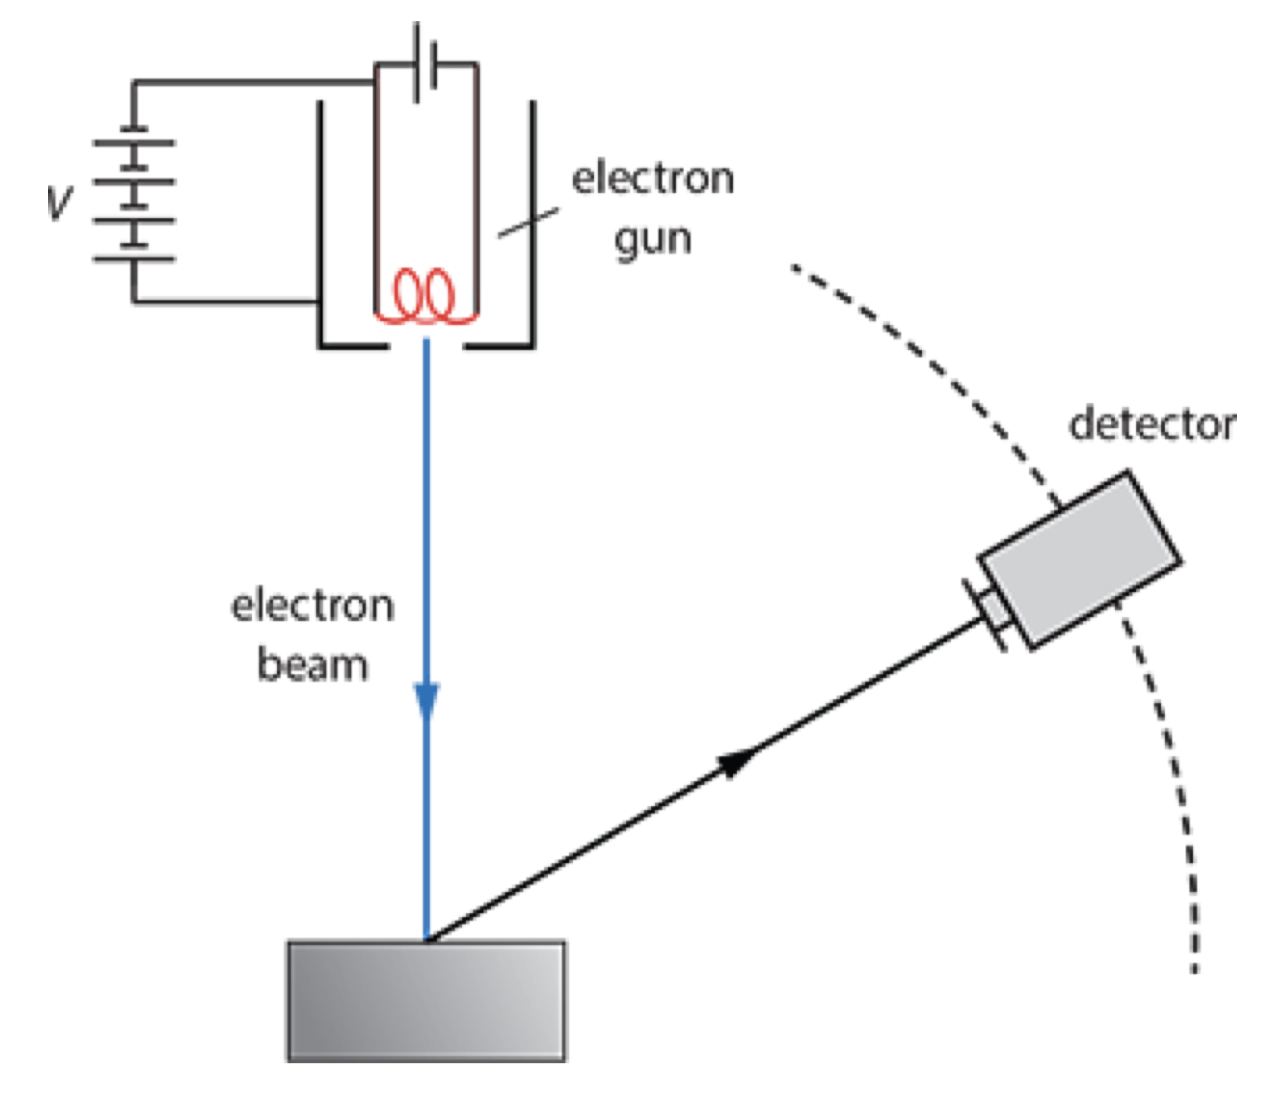
\includegraphics[width=0.4\linewidth]{Screenshot 2026-07-10 at 12.30.22.png}
  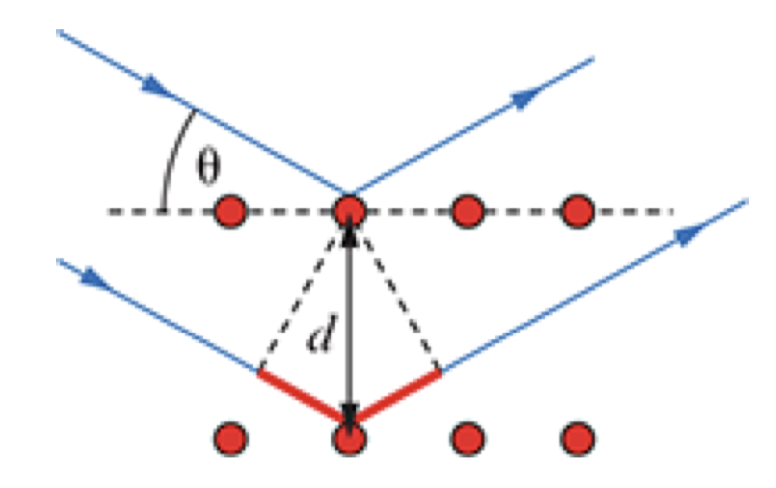
\includegraphics[width=0.3\linewidth]{Screenshot 2026-07-10 at 12.30.36.png}
\end{center}
\section{Nuclear physics}
\subsection{Mass defect and binding energy}
\subsubsection*{Nuclear notation}
Very \textit{professional vocabs}:
\begin{itemize}
  \item Nucleon: denotes a proton / neutron
  \item Proton number: number of protons, denoted as $Z$
  \item Nucleon number: number of protons + neutrons
  \item Number of neutrons: $N=A-Z$
  \item Electric charge of the nucleus: $eZ$, where $e=1.6\times 10^{-19}\ \text{C}$ is the charge of a proton
  \item $^A_ZX$ is the nucleus of element $X$.
  \item Nuclide: A nucleus with a specific number of protons and neutrons
\end{itemize}
A table of common particles and a summary of them:
\begin{center}
\begin{tabularx}{\textwidth}{@{}|Y | Y|@{}}
\toprule
\textbf{Particle} & \textbf{Symbol} \\
\midrule 
Proton, Antiproton & $^1_1p,\ ^1_{-1}\overline{p}$\\
\midrule
Neutron, Antineutron & $^1_0n,\ ^1_0\overline{n}$\\
\midrule
Electron, Positron & $^0_{-1}e,\ ^0_{+1}\overline{e}$\\
\midrule
Photon & $^0_0\gamma/\gamma$ \\
\midrule
Neutrino, Antineutrino & $^0_0\nu/\nu,\ ^0_0\overline{\nu}/\overline{\nu}$ \\
\midrule
Alpha particle & $^4_2\text{He}/^4_2\alpha$ \\
\bottomrule 
\end{tabularx}
\end{center}
\subsubsection*{(Four) Fundamental forces}
\begin{enumerate}
  \item The electromagnetic interaction: it acts on any particle that has electric charge. The force is given by Coulomb's law. It has infinite range.
  \item The weak nuclear interaction: it acts on protons, neutrons, electrons and neutrinos in order to bring about beta decay. It has very short range.
  \item The strong nuclear interaction: it acts on protons and neutrons to keep them bound to each other inside nuclei. It has short range
  \item The gravitational interaction: it acts on any particle with mass. The small mass of atomic particles makes this force irrelevant for atomic and nuclear physics. It has infinite range.
\end{enumerate}
\subsubsection*{Isotopes}
Nuclei of the same element have the same number of protons but may have different number of neutrons; these are called isotopes of each other. Since isotopes have the same number of protons, their atoms have the same number of electrons as well. This means that isotopes have identical chemical properties but different physical properties. The existence of isotopes is evidence for the existence of neutrons inside atomic nuclei.
\subsubsection*{The atomic mass unit}
Defined to be $\dfrac{1}{12}$ of the mass of carbon-12, $^{12}_6\text{C}$. The symbol for atomic mass unit is $u=1.6605402 \times 10^{-27}\ \text{kg}$.
\subsubsection*{The mass defect and binding energy}
Protons and neutrons are very tightly bound to each other in a nucleus through the action of the strong nuclear force. To separate them, energy must be supplied to the nucleus. Conversely, energy is released when a nucleus is assembled from its constituent nucleons.
In Einstein's theory of relativity, $E=mc^2$. Therefore, for a mass of 1u, the energy is 931.5 MeV. Since we must supply energy to a nucleus to separate the nucleons and since energy is equivalent to mass, it follows that the total mass of the separated nucleons is greater than the mass of the nucleus. The mass defect, $\mu$, is the total mass of the nucleons minus the mass of the nucleus.
\[
\begin{aligned}
\mu&=Zm_p+Nm_n-M_\text{nucleus}\\
&=Zm_p+Nm_n-(M_\text{atom}-Zm_e)\\
&=Z(m_p+m_e)+Nm_n-M_\text{atom}\\
&=Zm_\text{Hydrogen}+Nm_n-M_\text{atom}
\end{aligned}\]
The energy equivalent to the mass defect is called binding energy, $E_b=\mu c^2$.\\
The energy required to remove one nucleon from the nucleus is roughly the binding energy divided by the total number of nucleons. Thus, the binding energy per nucleon, $b$, is a measure of how tightly bound the nucleus is.
\subsubsection*{The binding energy curve}
\begin{center}
  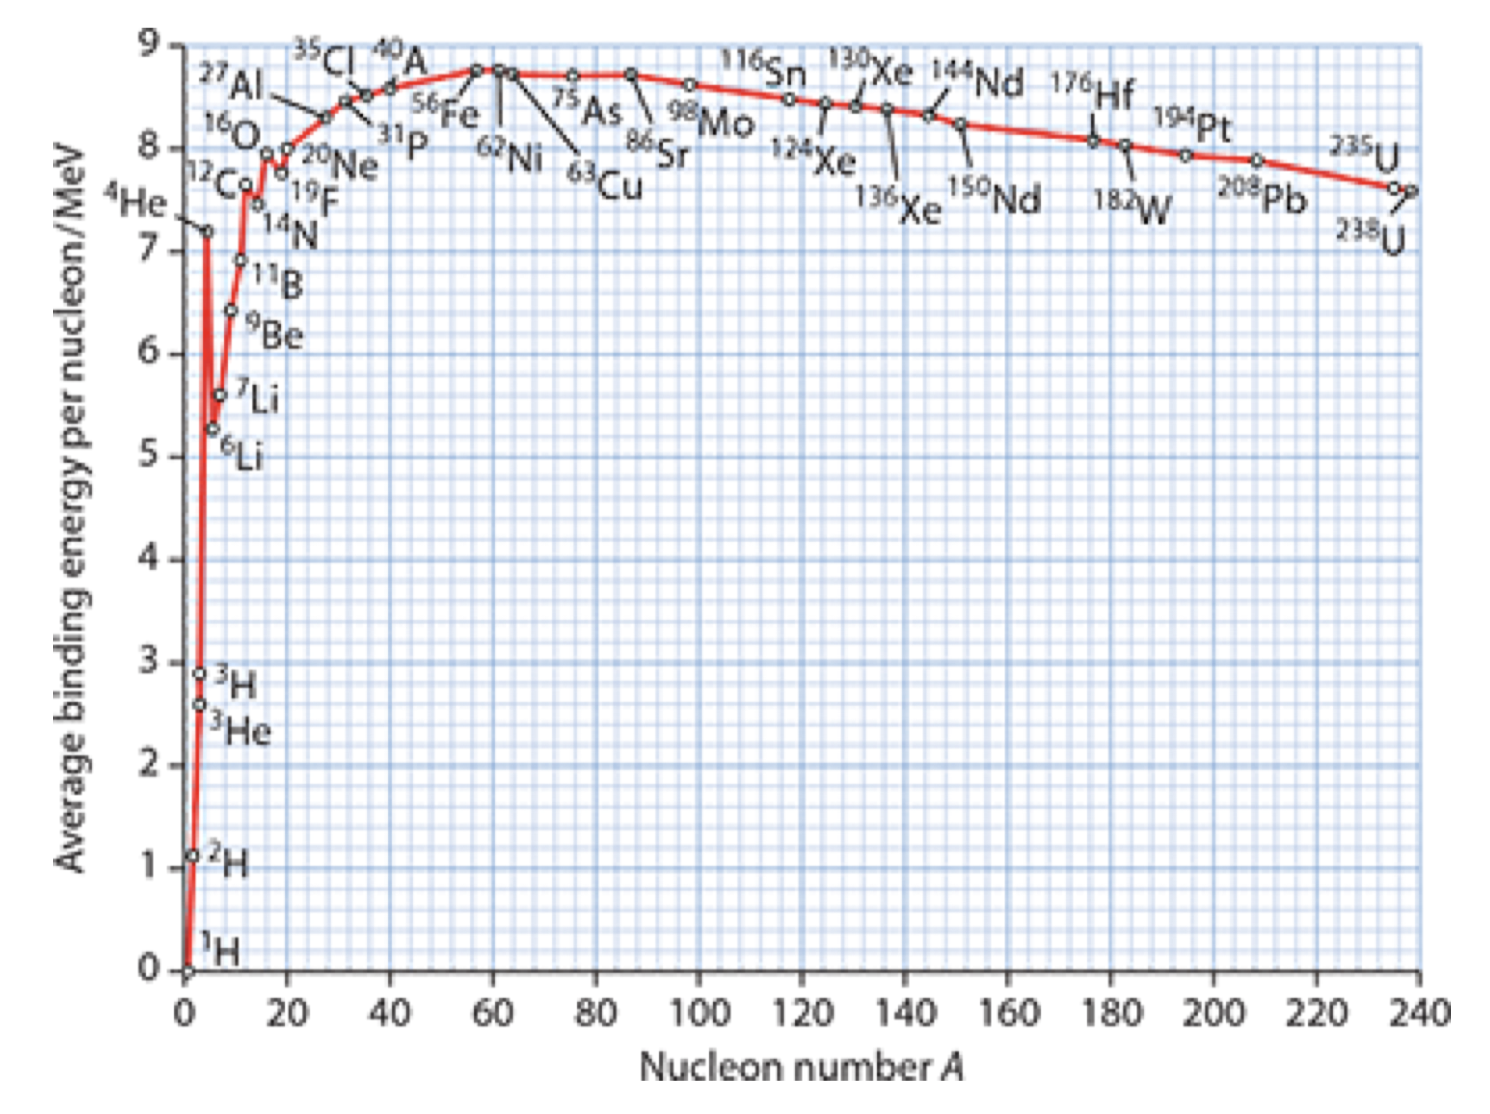
\includegraphics[width=0.6\linewidth]{Screenshot 2026-07-10 at 16.50.33.png}
\end{center}
\begin{itemize}
  \item The binding energy per nucleon for hydrogen is 0 because there is only one particle in the nucleus and there is nothing to separate.
  \item The curve rises sharply for low values of A.
  \item The curve has a maximum for A = 62 corresponding to nickel, which makes this nucleus particularly stable.
  \item There are peaks at the position of the nuclei $^4_2\text{He},^{12}_6\text{C},^{16}_8\text{O}$, which makes these nuclei unusually stable compared to their immediate neighbors.
  \item The curve drops gently from the peak at A = 62 and onwards.
  \item Most nuclei have a binding energy per nucleon between 7 and 9 MeV.
\end{itemize}
\subsubsection*{The energy released in nuclear reactions}
There's a conservation of electric charge and nucleon number for nuclear reaction (fusion or fission).\\
To decide whether energy is released in any nuclear reaction, we have to calculate the mass difference $\Delta m=m_\text{reactants}-m_\text{products}$. 
\begin{itemize}
  \item If $\Delta m>0$, then energy will be released and the decay will occur. 
  \item If $\Delta m<0$, the reactants will not react and the reaction can take place only if energy is supplied. 
\end{itemize}
The quantity of energy $Q$ released is the energy equivalent of the mass difference. This energy is released in the form of kinetic energy.
\subsection{Radioactivity}
\subsubsection*{Radioactive decays}
An unstable nucleus is one that randomly and spontaneously emits particles that carry energy away from the nucleus.
The emission of particles and energy from a nucleus is called radioactivity. Radioactive decay is random and spontaneous.
\subsubsection*{Properties of alpha, beta and gamma radiations}
\begin{center}
\begin{tabularx}{\textwidth}{@{}|Y |Y |Y| Y|@{}}
\toprule
\textbf{Characteristic} & \textbf{Alpha} & \textbf{Beta} & \textbf{Gamma} \\
\midrule
Nature & Helium nucleus & Fast electron & Photon\\
\midrule
Charge & +2e & -e & 0\\
\midrule
Mass & $6.64\times 10^{-27}\ \text{kg}$ & $9.1\times 10^{-31}\ \text{kg}$ & 0\\
\midrule
Penetrating power & A few cm of air & A few mm of metal & Many cm of lead \\\midrule
Ions per mm of air for 2 MeV particles & 10000 & 100 & 1\\\midrule
Description & An alpha particle is emitted from the parent nucleus creating the daughter nucleus. 
& $\beta^-:$ a neutron turns into a proton, emitting an electron and an anti-neutrino. $\beta^+$: the nucleus emits positron and neutrino. 
& In gamma decay a nucleus emits a gamma ray, a photon of high-$f$ EM radiation. $\lambda$ of the photon emitted is $\lambda=\dfrac{hc}{E}$.\\\midrule
Detection & Affects photographic film & Affects photographic film & Affects photographic film\\
 & Is affected by electric and magnetic fields & Is affected by electric and magnetic fields &Is not affected by electric and magnetic fields\\
\bottomrule
\end{tabularx}
\end{center}
\subsubsection*{The law of radioactive decay}
The law of radioactive decay states that the rate of decay is proportional to the number of nuclei that have not yet decayed: $\dfrac{\Delta N}{\Delta t}\propto N$.
A consequence of this law is that the number of radioactive nuclei decreases exponentially.\\\\
Half-life: the time after which the number of the radioactive nuclei is reduced by a factor of 2, or the interval of time after which the activity ($A$, number of decays, unit Bq= 1 decay / s) of a radioactive sample is reduced by a factor of 2.\\
Background radiation sources: cosmic rays from the sun, radioactive material in rocks and the ground, radiation from nuclear weapons testing grounds etc. that provides background radiation.
\subsubsection*{Half-life and probability}
The meaning of a half-life can also be understood in terms of probability. Any given nucleus has a 50\% chance of decaying within a time interval equal to the half-life. If a half-life goes by and the nucleus has not decayed, the chance that it will decay in the next half-life is still 50\%.
\begin{center}
  \begin{tikzpicture}[>=stealth, font=\small]

    % =========================================================================
    % LEFT DIAGRAM: RADIOACTIVE DECAY PROBABILITY TREE
    % =========================================================================
    \begin{scope}[xshift=0cm, yshift=1.5cm]
        
        % Style for tree nodes
        \tikzset{treenode/.style={circle, fill=red!80!black, draw=black, inner sep=0pt, minimum size=0.35cm}}
        
        % Nodes
        \node[treenode] (N0) at (0, 2) {};
        \node[treenode] (N1) at (2.5, 3.5) {};
        
        % Branches from First Node
        \draw[blue!70!black, thick, ->] (N0) -- (N1) 
            node[midway, above left, black] {does not decay};
            
        \draw[blue!70!black, thick, ->] (N0) -- (2.5, 0.5) 
            node[midway, below left, black] {decays};
            
        % Branches from Second Node
        \draw[blue!70!black, thick, ->] (N1) -- (5, 4.7) 
            node[midway, above left, black] {does not decay};
            
        \draw[blue!70!black, thick, ->] (N1) -- (5, 2.3) 
            node[midway, below left, black] {decays};
        % Bottom Timeline / Half-life intervals
        \draw[thick, <->] (0, -0.8) -- (2.5, -0.8) node[midway, below] {half-life};
        \draw[thick, <->] (2.5, -0.8) -- (5, -0.8) node[midway, below] {half-life};
        \draw[dashed, black!30] (0,0.2) -- (0, -0.7);
        \draw[dashed, black!30] (2.5,0.2) -- (2.5, -0.7);
        \draw[dashed, black!30] (5,2.1) -- (5, -0.7);

    \end{scope}

    % =========================================================================
    % RIGHT DIAGRAM: SEGRÈ PLOT / DECAY CHAIN (A vs Z)
    % =========================================================================
    \begin{scope}[xshift=8.5cm, yshift=0cm, x=0.5cm, y=0.18cm]
        
        % Mid-arrow decoration styles
        \tikzset{
            alpha/.style={red!90!black, thick, decoration={markings, mark=at position 0.55 with {\arrow{Latex[scale=0.8]}}}, postaction={decorate}},
            beta/.style={blue!80!black, thick, decoration={markings, mark=at position 0.65 with {\arrow{Latex[scale=0.8]}}}, postaction={decorate}}
        }

        % --- Grid Lines ---
        \foreach \y in {0,1,...,32} {
            \draw[cyan!15, ultra thin] (0,\y) -- (12,\y);
        }
        \foreach \y in {0,4,...,32} {
            \draw[cyan!35, thin] (0,\y) -- (12,\y);
        }
        \foreach \x in {0,1,...,12} {
            \draw[cyan!35, thin] (\x,0) -- (\x,32);
        }

        % --- Axes ---
        \draw[thick] (0,0) -- (12.5,0) node[below right, yshift=-4pt] {$Z$};
        \foreach \z [count=\x from 0] in {80,81,...,92} {
            \draw[thick] (\x, 0) -- (\x, -0.5) node[below, font=\footnotesize] {\z};
        }
        
        \draw[thick] (0,0) -- (0,33) node[above left, xshift=-4pt] {$A$};
        \foreach \a [count=\i from 0] in {200,204,...,232} {
            \pgfmathsetmacro{\ypos}{\i * 4}
            \draw[thick] (0, \ypos) -- (-0.3, \ypos) node[left, font=\footnotesize] {\a};
        }

        % --- Plotting Decay Paths ---
        \draw[alpha] (10, 32) -- (8, 28);  % Th-232 -> Ra-228
        \draw[alpha] (10, 28) -- (8, 24);  % Th-228 -> Ra-224
        \draw[alpha] (8, 24) -- (6, 20);   % Ra-224 -> Rn-220
        \draw[alpha] (6, 20) -- (4, 16);   % Rn-220 -> Po-216
        \draw[alpha] (4, 16) -- (2, 12);   % Po-216 -> Pb-212
        
        \draw[beta] (8, 28) -- (9, 28);    % Ra-228 -> Ac-228
        \draw[beta] (9, 28) -- (10, 28);   % Ac-228 -> Th-228
        
        \draw[beta] (2, 12) -- (3, 12);    % Pb-212 -> Bi-212
        
        % Branch 1
        \draw[beta] (3, 12) -- (4, 12);    % Bi-212 -> Po-212
        \draw[alpha] (4, 12) -- (2, 8);    % Po-212 -> Pb-208
        
        % Branch 2
        \draw[alpha] (3, 12) -- (1, 8);    % Bi-212 -> Tl-208
        \draw[beta] (1, 8) -- (2, 8);      % Tl-208 -> Pb-208

        % --- Data Markers ---
        \foreach \z/\a in {
            10/32, 8/28, 9/28, 10/28, 8/24, 6/20, 4/16, 2/12, 3/12, 4/12, 1/8, 2/8
        } {
            \fill[black] (\z, \a) circle (2.2pt);
        }

        % --- Legend ---
        \begin{scope}[shift={(6.2, 2)}]
            \draw[cyan!35, fill=white] (0,0) rectangle (5.5, 4.5);
            \draw[beta] (0.3, 3) -- (1.5, 3);
            \node[right, font=\footnotesize] at (1.6, 3) {beta minus decay};
            \draw[alpha] (0.3, 1.2) -- (1.5, 1.2);
            \node[right, font=\footnotesize] at (1.6, 1.2) {alpha decay};
        \end{scope}

    \end{scope}

\end{tikzpicture}
\end{center}
\subsection{Nuclear properties and the radioactive decay law}
\subsubsection*{Nuclear radii}
When an alpha particle of kinetic energy $E_K$ is directed at a nucleus of proton number $Z$, the distance of closest approach, $d$, is found by equating the kinetic energy far from the nucleus to the electric potential energy at the point of closest approach.
\[E_K=k\dfrac{(2e)(Ze)}{d}\Rightarrow d=\frac{2kZe^2}{E_K}\]
\begin{center}
\begin{tikzpicture}[>=stealth, font=\small]
    
    % Custom color palette matching the original style
    \definecolor{particleblue}{RGB}{52, 152, 219}
    \definecolor{nucleusorange}{RGB}{211, 124, 63}
    
    % =========================================================================
    % TOP DIAGRAM: Incident Particle approaching from far away
    % =========================================================================
    \begin{scope}[yshift=2.5cm]
        % Horizontal impact parameter centerline
        \draw[dashed, thick, black!70] (0,0) -- (6,0);
        
        % Incoming alpha particle / projectile
        \filldraw[fill=particleblue, draw=black!80, thick] (0,0) circle (0.16cm);
        
        % Velocity arrow above the particle
        \draw[thick, ->] (-0.3, 0.35) -- (0.4, 0.35);
        
        % Target Heavy Nucleus
        \filldraw[fill=nucleusorange, draw=black!80, thick] (6,0) circle (0.85cm);
    \end{scope}
    
    % =========================================================================
    % BOTTOM DIAGRAM: Particle momentarily at rest at distance 'd'
    % =========================================================================
    \begin{scope}[yshift=0cm]
        % Target Heavy Nucleus
        \filldraw[fill=nucleusorange, draw=black!80, thick] (6,0) circle (0.85cm);
        
        % Alpha particle at the instantaneous turning point
        \filldraw[fill=particleblue, draw=black!80, thick] (3.8,0) circle (0.16cm);
        
        % Reversal/recoil indicator arrow (pointing left away from nucleus)
        \draw[thick, ->] (3.8, 0) -- (3.1, 0);
        
        % Velocity label at turning point
        \node[above, yshift=4pt] at (3.8, 0) {$v = 0$};
        
        % Distance of closest approach 'd' (from particle center to nucleus center)
        \draw[thick, <->] (3.8, 0) -- (6, 0) node[midway, above, yshift=1pt] {$d$};
    \end{scope}
    
\end{tikzpicture}
\end{center}
As the energy of the incoming alpha particles increases, the distance of closest approach decreases and will eventually approach the nuclear surface. \\\\
When the alpha particle is near the nuclear surface deviations from Rutherford scattering will be observed because the nuclear force will start acting on the alpha particle. The number of scattered alpha particles will not be what is expected based on Rutherford scattering. Thus, the distance of closest approach measured in this case will essentially be the nuclear radius.\\\\
The radius of a nucleus is given by $R=R_0 A^{1/3}$, where $R_0\approx 1.2\times 10^{-15}\ \text{m}$ and $A$ is the nucleon number. (This formula also implies that the volume of a nucleus is proportional to the number of nucleons in it, and that the density of nuclei is constant, $\rho=2\times 10^{17}\ \text{kg\,m}^{-3}$.)
\subsubsection*{Deviations from Rutherford scattering — evidence for the strong nuclear force}
The Rutherford formula states that as the scattering angle increases, the number of alpha particles scattered at that angle decreases very sharply.
It states that the number $N$ of alpha particles scattering at an angle $\theta$ is proportional to $\dfrac{1}{\sin^4(\theta/2)}$. (If this was the case, $N\sin^4\left(\dfrac{\theta}{2}\right)$ would be a constant for all angles of $\theta$.)\\\\
The derivation of the Rutherford formula is based on a number of assumptions. The most important is that the only force in play during the scattering process is the electric force. As the energy of the alpha particles increases, the alpha particles can get closer to the nucleus. When the distance of closest approach gets to be
about $10^{-15}$ m or less, deviations from the Rutherford formula are observed. This is due to the fact that the alpha particles are so close to the nucleus that the strong nuclear force begins to act on the alpha particles. 
\begin{center}
  \begin{tikzpicture}

\begin{axis}[
    width=13cm,
    height=7cm,
    xmin=15,xmax=40,
    ymin=0,ymax=5,
    axis lines=left,
    xlabel={$E\;/\text{MeV}$},
    ylabel={$\log N$},
    xlabel style={at={(axis description cs:1.02,-0.04)},anchor=north west},
    ylabel style={at={(axis description cs:-0.06,1.02)},anchor=south},
    xtick={15,20,25,30,35,40},
    ytick={0,1,2,3,4,5},
    minor tick num=4,
    grid=both,
    major grid style={blue!40,line width=0.5pt},
    minor grid style={blue!15,line width=0.3pt},
    tick style={black,thick},
    axis line style={thick},
    enlargelimits=false,
]

% Original spectrum (solid blue)
\addplot[
    very thick,
    blue
]
coordinates{
    (15,3.75)
    (27.5,2.55)
    (38,0)
};

\addplot[
    red,
    very thick,
    dashed,
    smooth
] coordinates {
    (15,3.75)
    (18,3.45)
    (21,3.15)
    (24,2.88)
    (27.5,2.55)
    (30,2.40)
    (33,2.22)
    (36,2.03)
    (40,1.80)
};
\end{axis}

\end{tikzpicture}
\end{center}
The dotted curve is based on Rutherford scattering. The blue curve is the observed curve. We see deviations when the energy exceeds about 28 MeV. The energy at which deviations start may be used to estimate the nuclear radius.
\subsubsection*{Approximate constancy of the binding energy per nucleon}
The short range of the force implies that a given nucleon can interact with its immediate neighbours only and not with all of
the nucleons in the nucleus. So, for large nuclei (roughly A > 20) any one nucleon is surrounded by the same number of immediate neighbours, and so the energy needed to remove that nucleon from the nucleus is the same. 
\begin{center}
  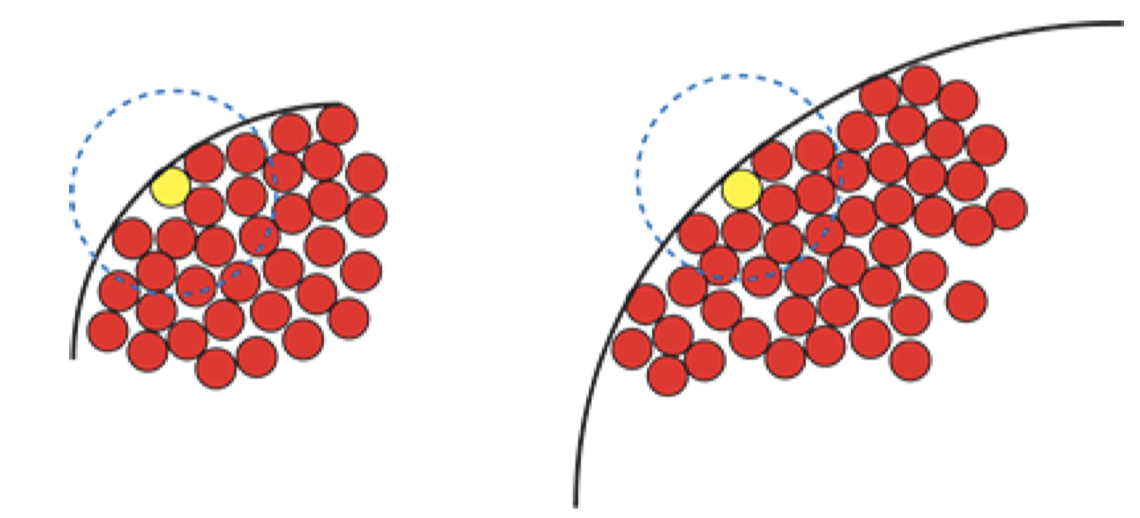
\includegraphics[width=0.8\linewidth]{Screenshot 2026-07-11 at 09.07.54.png}
\end{center}
\subsubsection*{Nuclear stability - the role of neutrons}
\begin{center}
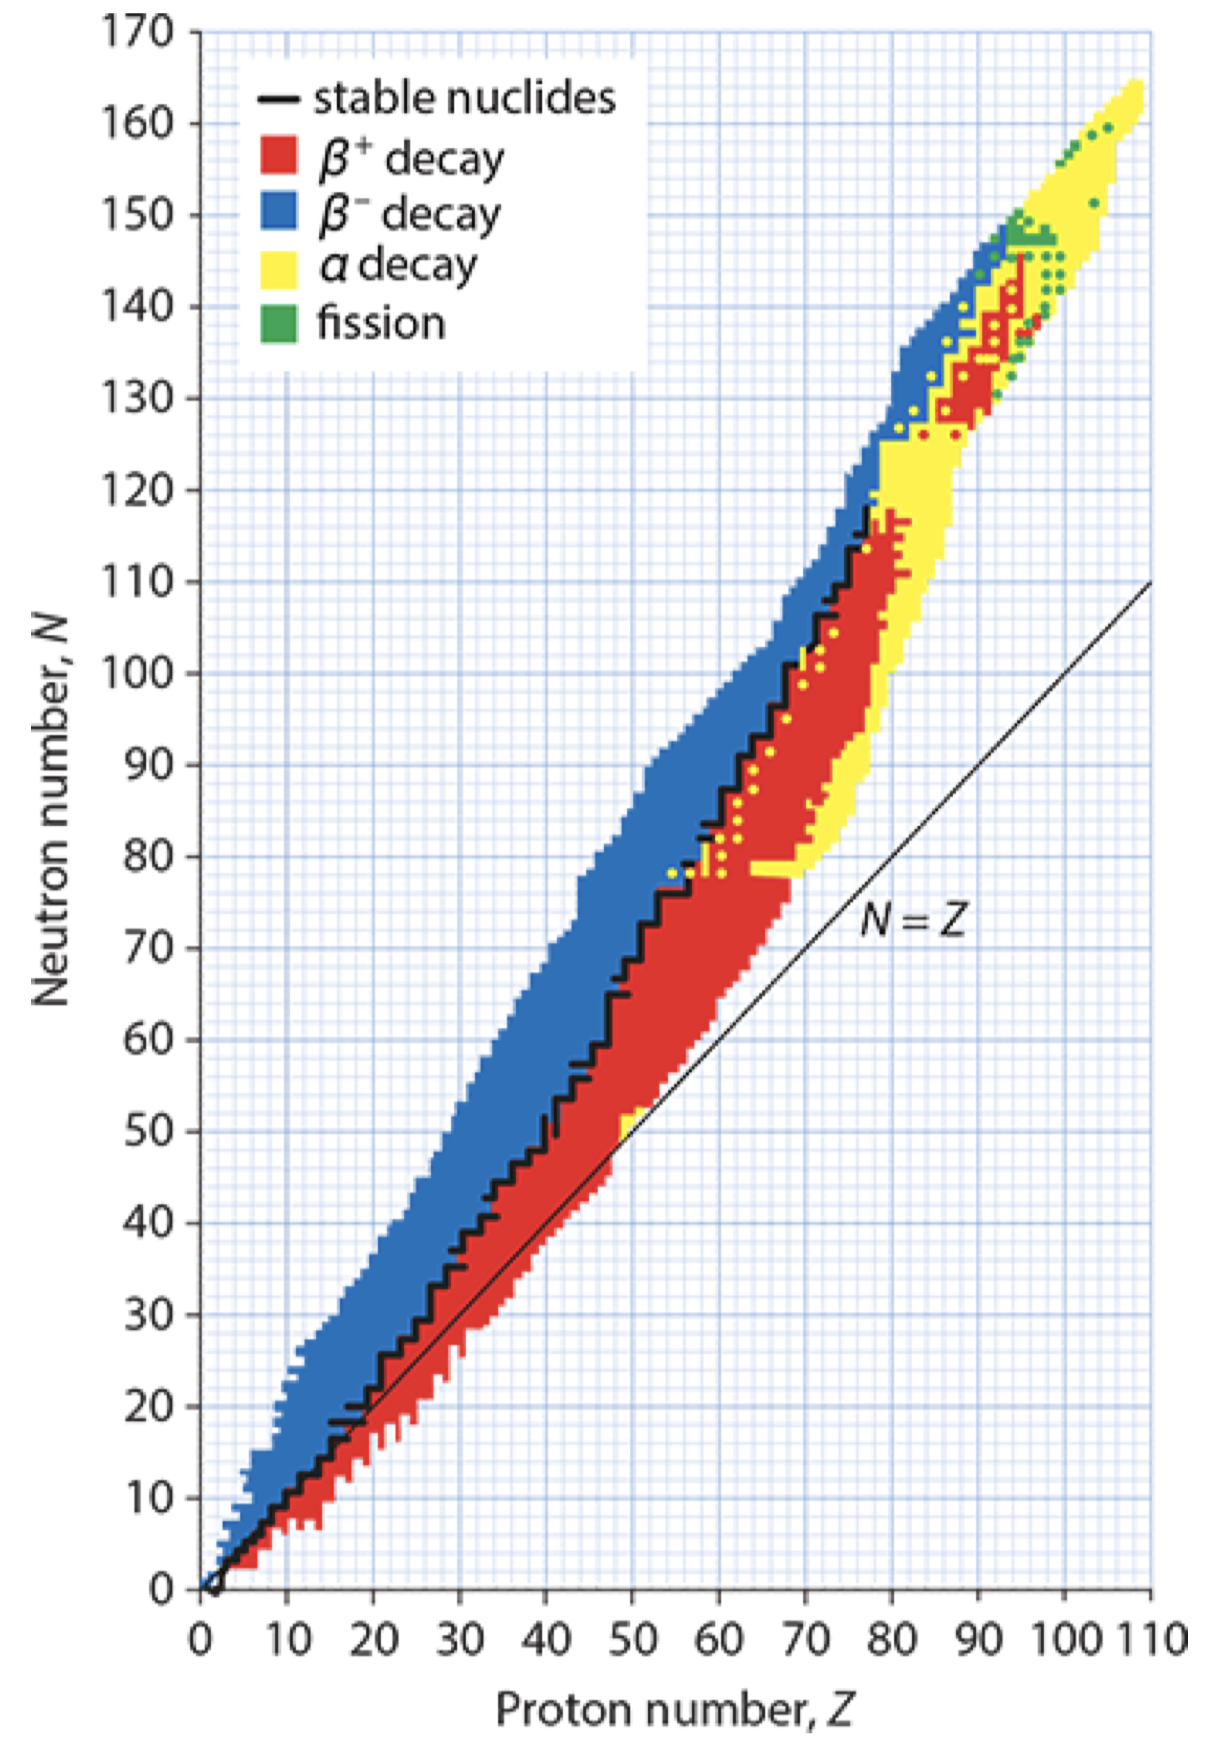
\includegraphics[width=0.55\linewidth]{Screenshot 2026-07-11 at 09.20.36.png}
\end{center}
Notice that stable nuclei with small values of $Z$ have equal numbers of neutrons and protons. As $Z$ increases, stable nuclei have more neutrons than protons, both because the extra neutrons make the distance between protons larger (EM force acts on protons, and it is repulsive, acts on infinite range, increasing the tendency for the nucleus to break apart. The strong nuclear force does not help because for large enough nuclei the number of nearest neighbours of a given proton is the same and because of the short range of the force only these act on a given proton.) and because the neutrons contribute to binding.
\subsubsection*{Nuclear energy levels}
The nucleus, like the atom, exists in discrete energy levels. The main evidence for the existence of nuclear energy levels comes from the fact that the energies of the alpha particles and gamma ray photons that are emitted by nuclei in alpha and gamma decays are discrete. This is to be contrasted with beta decays, in which the electron has a continuous range of energies.
\subsubsection*{The neutrino}
The IG / 1930s version of the beta minus decay can be given by
\[^1_0n\rightarrow ^1_1p+^0_{-1}e\]
It has a mass difference $\Delta m=0.00084\ \text{u}$ and energy of $Q=0.783\ \text{MeV}$.
If only the electron and the proton are produced, then the electron, being the lighter of the two, will carry most of this energy away as kinetic energy. \\
To see this, assume that the neutron is at rest when it decays. Then the total momentum before the decay is zero. After the decay the electron and the proton will have equal and opposite momenta, each of magnitude $p$. Equating the total $E_K$ after the decay to the energy released, $Q$:
\[
\begin{aligned}
  \dfrac{p^2}{2m_e}+\dfrac{p^2}{2m_p}&=Q\\
  p^2\left(\dfrac{1}{2m_e}+\dfrac{1}{2m_p}\right)&=Q\\
  p^2&=\dfrac{2Qm_em_p}{m_e+m_p}\\
  E_K&=\dfrac{p^2}{2m_e}=\dfrac{Qm_p}{m_e+m_p}\approx Q
\end{aligned}\]
Thus, we should observe electrons with kinetic energies of about 0.783 MeV. In experiments, however, the electron has a \textbf{range} of energies 0 to 0.783 MeV.
It means that a third very light particle must also be produced so that it carries the remainder of the available energy, and it is named "neutrino", $\nu$. Some properties:
\begin{itemize}
  \item Electrically neutral
  \item Negligible mass, gravitational interaction is negligible
  \item No strong nuclear interaction
\end{itemize}
\subsubsection*{The radioactive decay law}
The rate of decay is proportional to the number of nuclei present that have not yet decayed,
\[\dfrac{dN}{dt}=-\lambda N\]
The decay constant is $\lambda=\dfrac{\text{probability of decay per unit time}}{dt}$, the constant of proportionality / probability of decay per unit time. The solution to this differential equation is
\[N(t)=N_0e^{-\lambda t}\]
where $N_0$ is the initial number of nuclei.\\
The (negative) rate of decay (i.e. the number of decays per second) is called activity, A:
\[A=-\dfrac{dN}{dt}=\lambda N_0e^{-\lambda t}=\lambda N;\ A_0=\lambda N_0\]
A graph of A against N gives a straight line whose slope is the decay constant.\\
The relationship of half-life and decay constant is given by
\[\lambda T_{1/2}=\ln 2\]
\section{Nuclear fission}
\subsection{Nuclear fission}
Nuclear fission is the process in which a heavy nucleus splits up into two lighter nuclei. The production of neutrons is a key feature of fission reactions. The energy released appears as kinetic energy of the products, mostly for the produced neutrons. 
\begin{enumerate}
  \item This can happen when the nucleus is bombarded by a neutron, and in this case we speak of \textbf{induced fission}.
  \item In \textbf{spontaneous fission}, a nucleus may split into two smaller nuclei without neutron absorption.
\end{enumerate}
\subsubsection*{Fission and the binding energy curve}
The energy released, other than calculating mass difference, can also be calculated by subtracting from the total binding energy on the right of the reaction the total binding energy on the left of the reaction.\\\\
The energy released in terms of binding energy per nucleon, $b$, is expressed as
\[Q=\sum N(b_{\text{products}}-b_{\text{reactants}})\]
where $N$ is the number of nucleons in the nucleus. \\
For fission, the products will be at the left of the reactants on the energy binding curve, and thus $b_{\text{products}}>b_{\text{reactants}}$, so $Q>0$, indicating energy release. 
Fission means heavy nuclei split into lighter nuclei with higher binding energy per nucleon. Fusion means light nuclei join to form heavier nuclei with higher binding energy per nucleon. 
\begin{center}
  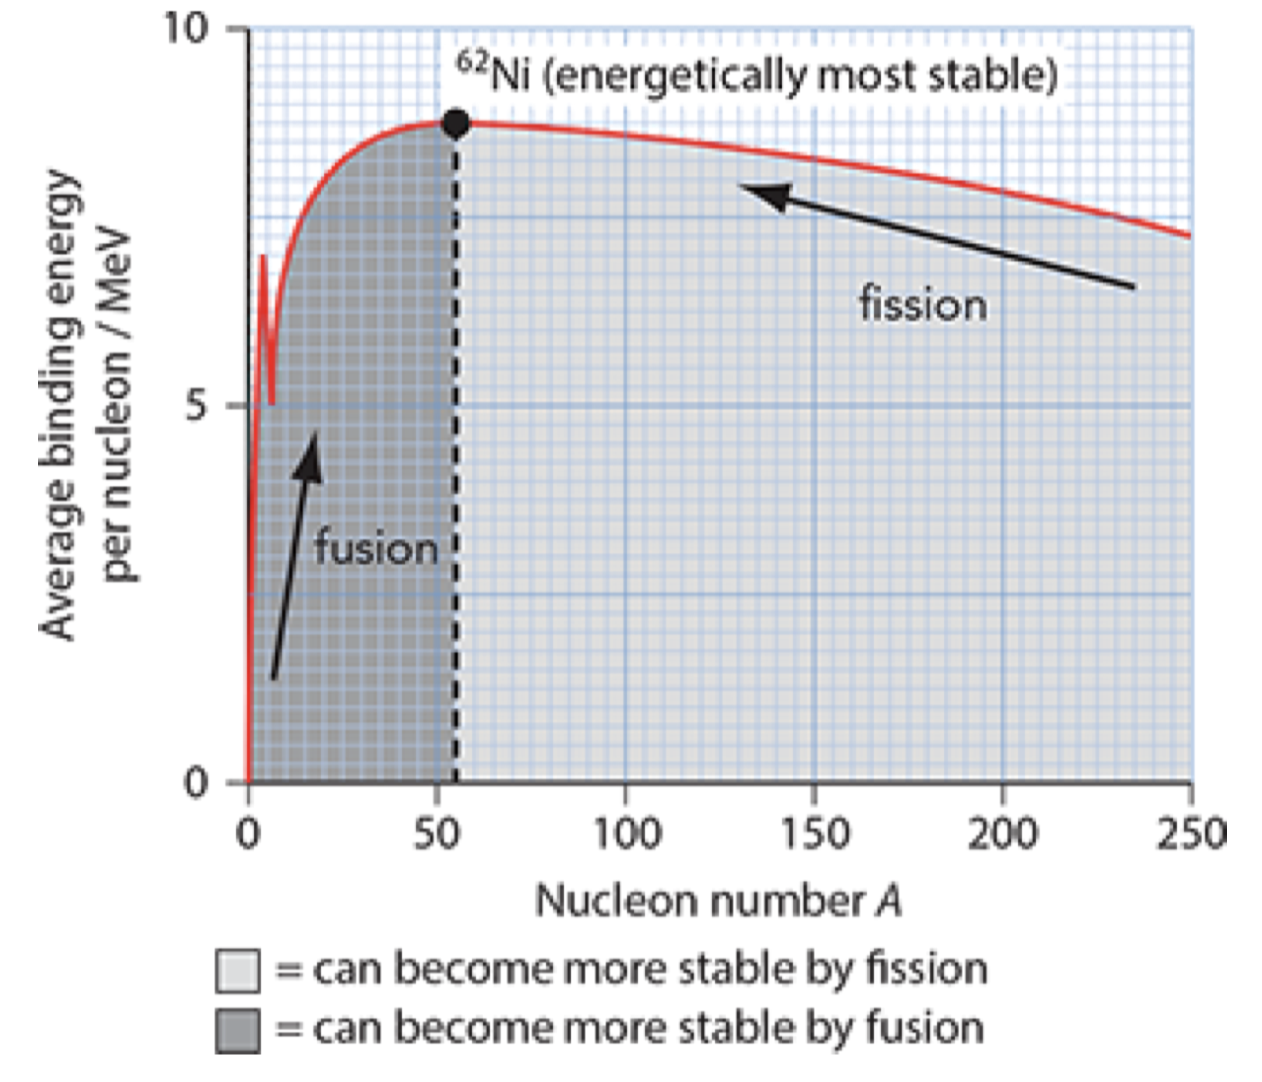
\includegraphics[width=0.6\linewidth]{Screenshot 2026-07-11 at 10.09.30.png}
\end{center}
\subsubsection*{Nuclear fission reactors}
A nuclear reactor is a machine in which nuclear fission reactions take place, producing energy. The fuel of a nuclear reactor is typically uranium-235. Neutrons initiate the reaction. One possible fission reaction is:
\[^1_0n + ^{235}_{92}\text{U} \rightarrow ^{140}_{54}\text{Xe} + ^{94}_{38}\text{Sr} + 2^1_0n\]
\begin{center}
  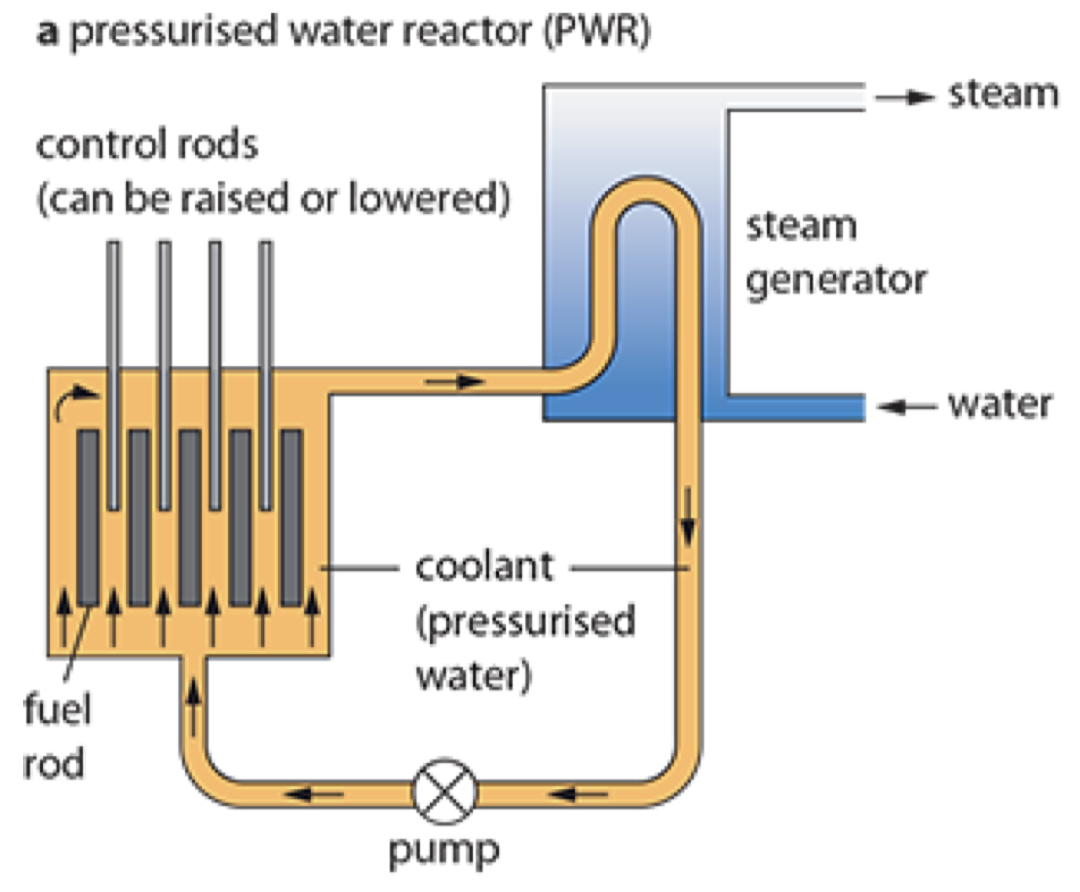
\includegraphics[width=0.45\linewidth]{Screenshot 2026-07-11 at 10.28.24.png}
  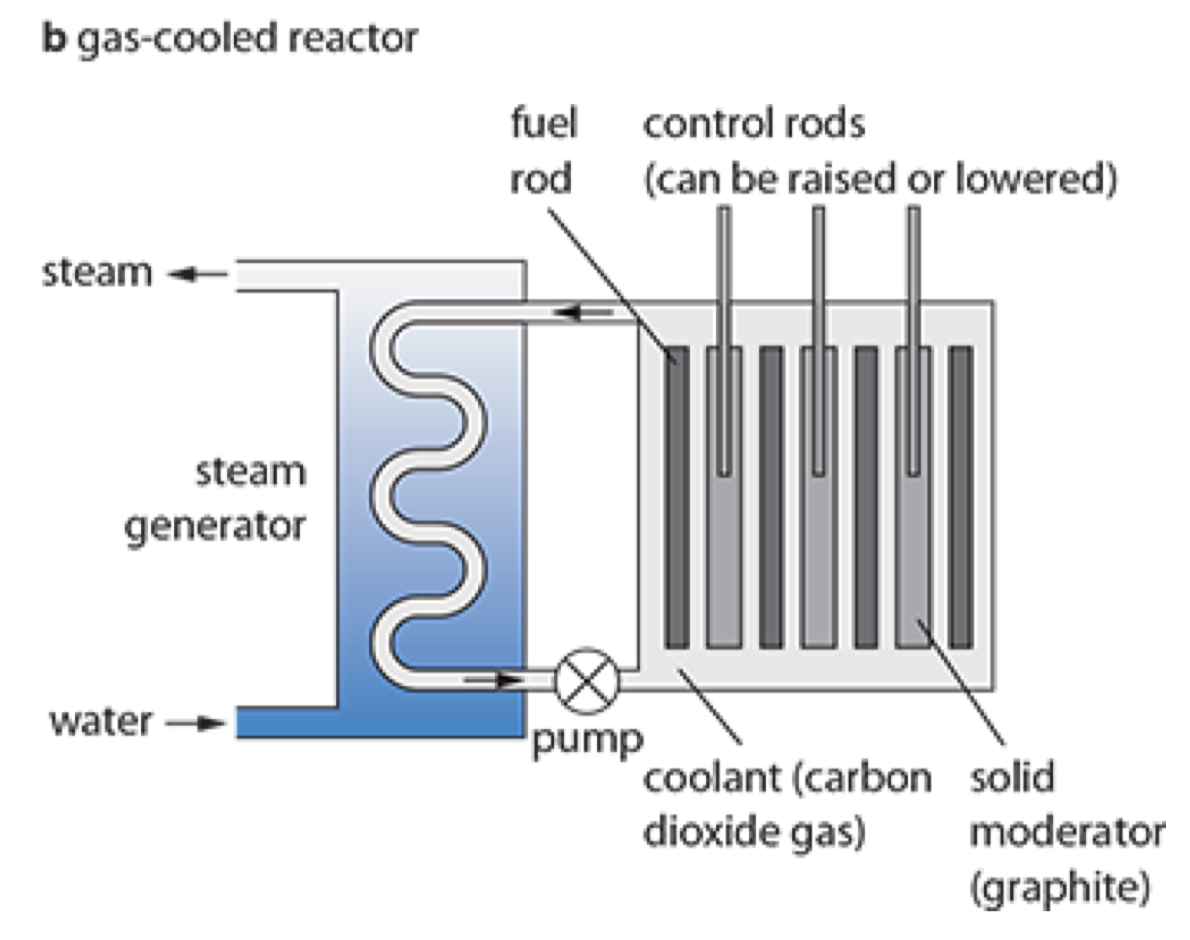
\includegraphics[width=0.45\linewidth]{Screenshot 2026-07-11 at 10.28.31.png}
\end{center}
The neutrons produced can be used to collide with other nuclei of uranium-235 in the reactor, producing more fission, more energy and more neutrons. The reaction is thus self-sustaining, called a chain reaction.\\
For the chain reaction to get going, a certain minimum mass, called the critical mass (about 15kg for pure uranium-235), of uranium-235 must be present, otherwise the neutrons escape without causing further reactions.
\begin{itemize}
  \item \textbf{A moderator} must be used so that it can slow down the neutrons produced in the fission reaction. This is because the neutrons produced are fast neutrons, and they are less likely to cause further fission reactions (not captured by uranium-235). The moderator is typically water or graphite.
  \item \textbf{Control rods} are used to absorb excess neutrons and thus control the rate of the reaction. The control rods are made of materials that absorb neutrons, such as boron or cadmium. The control rods can be raised or lowered into the reactor core to control the rate of fission.
  \item \textbf{A heat exchanger} is needed to decrease the temperature of the moderator (due to the energy increment caused by neutrons colliding with the moderator). This can be done using cold water that circulates in pipes throughout the moderator. 
\end{itemize}
The water is turned into steam at high temperature and pressure. The steam is then used to turn the turbines of a generator, finally producing electricity.\\\\
The rate of the reactions is determined by the number of neutrons available to be captured by uranium-235.
\begin{itemize}
  \item Too few neutrons would result in the reactions stopping.
  \item Too many neutrons would lead to an uncontrolled chain reaction, which is dangerous.
\end{itemize}
\subsubsection*{Risks with nuclear power}
The fast neutrons produced may be used to bombard uranium-238 and produce plutonium-239.
\[
\begin{aligned}
^1_0n + ^{238}_{92}\text{U} &\rightarrow ^{239}_{92}\text{U}\\
^{239}_{92}\text{U} &\xrightarrow{\beta^-} ^{239}_{93}\text{Np}\\
^{239}_{93}\text{Np} &\xrightarrow{\beta^-} ^{239}_{94}\text{Pu}
\end{aligned}\]
\begin{itemize}
  \item The plutonium-239 produced can then be used as the nuclear fuel in other reactors. It can also be used in the production of nuclear weapons, which therefore raises serious concerns.
  \item The spent fuel in a nuclear reactor and the products of the reactions are all highly radioactive with long half-lives. Radioactive waste is broadly classified as higher level and low level waste.
  \begin{itemize}
    \item Higher level waste is mainly the left-over uranium fuel in a reactor's fuel rods and the lighter elements produced in the fission of the uranium fuel. These elements are highly radioactive. The radiation produced when they decay is very penetrating and delivers fatal doses even during short exposures, decades after they have been removed from the reactor.
    \item Low level waste includes material that has become radioactive due to neutron absorption or has been contaminated with radioactive material. 
  \end{itemize}
  \item There is always the possibility of an accident due to uncontrolled heating of the moderator, which might start a fire or explosion. In the event of an explosion, radioactive material would leak from the sealed core of a reactor, dispersing radioactive material into the environment.
\end{itemize}
\begin{center}
\begin{tabularx}{\textwidth}{@{}|Y |Y |@{}}
\toprule
\textbf{Advantages} & \textbf{Disadvantages}\\
\midrule
High power output & Radioactive waste products difficult to dispose of\\
\midrule
Large reserves of nuclear fuels & Major public health hazard should 'something go wrong'\\
\midrule
No greenhouse gas emissions & Problems associated with uranium mining\\
\midrule
No acid rain & Possibility of producing materials for nuclear weapons\\
\bottomrule
\end{tabularx}
\end{center}
\section{Nuclear fusion and stars}
\subsection{Nuclear fusion}
Nuclear fusion is the joining of two light nuclei into a heavier one with the associated production of energy. 
\subsubsection*{Conditions for fusion to take place}
\begin{itemize}
  \item Temperature
  \begin{itemize}
    \item For fusion to occur, the reacting nuclei must join. 
    \item But nuclei are positively charged so they repel each other.
    \item At high temperatures (namely, millions of degrees, at plasma state already (electrons left atom)) the nuclei would be moving fast enough to overcome the Coulomb repulsion and crash into each other.
  \end{itemize}
  \item Density
  \begin{itemize}
    \item The number density of the nuclei (number of nuclei per unit volume) must be high so that there are lots of them around for fusion to occur.
  \end{itemize}
  \item Confinement time (not easy to be satisfied)
  \begin{itemize}
    \item The nuclei must be maintained at high temperature and density for a time long enough for many fusion reactions to take place.
  \end{itemize}
\end{itemize}
Nuclear fusion provides the energy that is radiated by stars into space, the pressure to keep a star from collapsing under its own weight and the nuclear fusion reactions and related processes that are responsible for nucleosynthesis, the creation of the chemical elements. 
\subsection{Stellar properties and the Hertzsprung-Russell diagram}
\subsubsection*{The Hertzsprung-Russell diagram}
In this diagram, luminosity (given in terms of the sun's luminosity, $L_\odot =3.9\times10^{26}$W)was plotted on the vertical axis and surface temperature (in K) on the horizontal axis. The slanted dotted lines represent stars with the same radius. $R_\odot$ stands for the sun's radius.
\begin{center}
  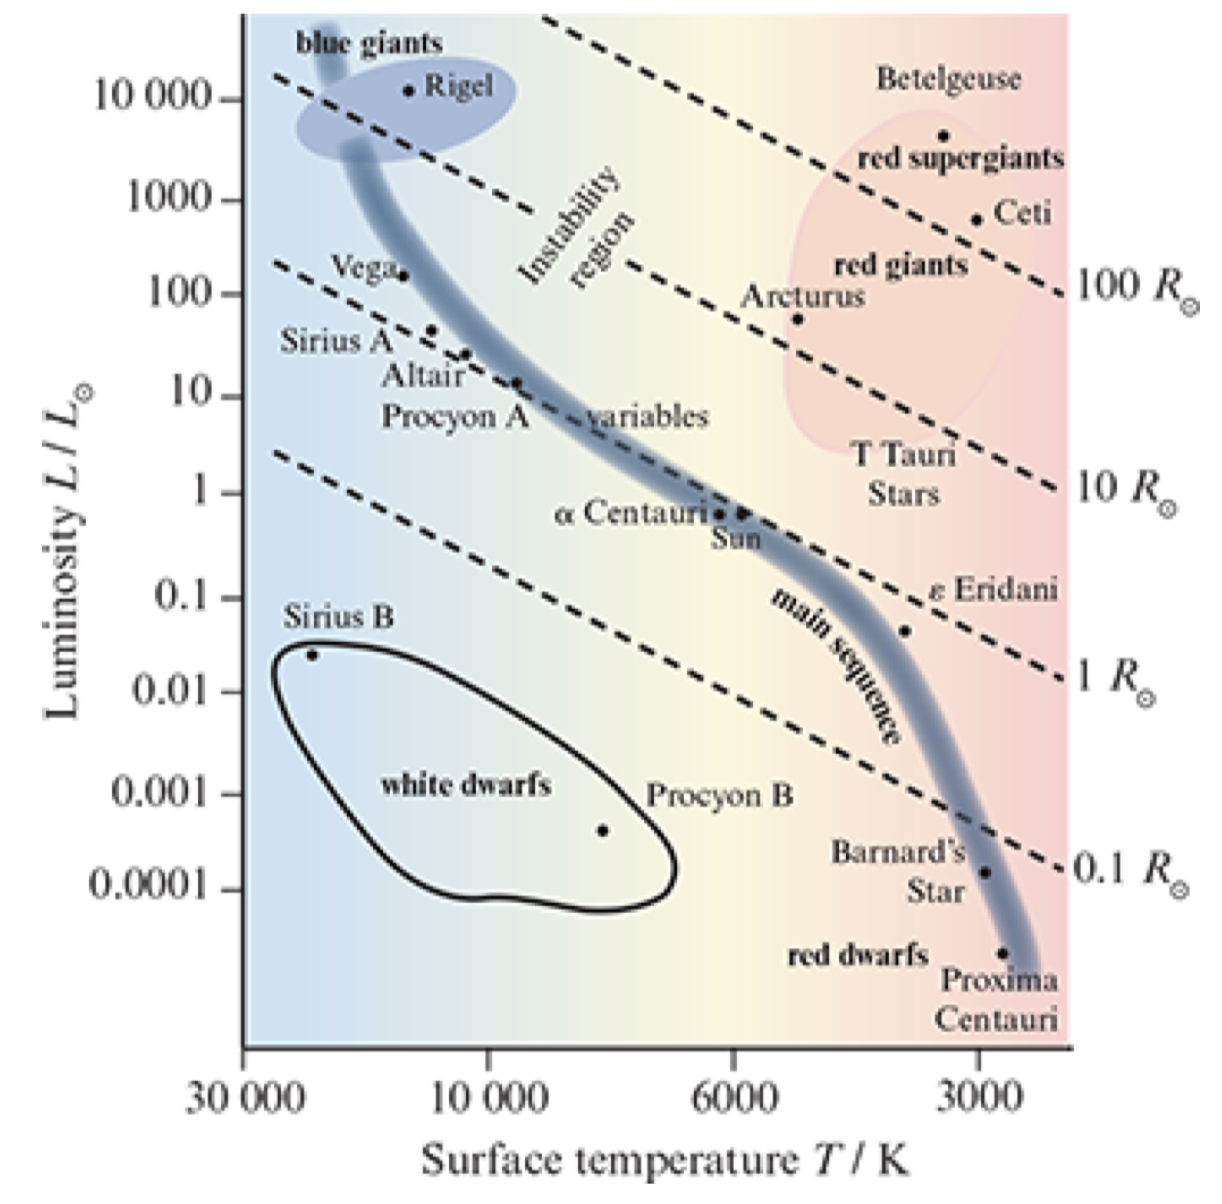
\includegraphics[width=0.6\linewidth]{Screenshot 2026-07-11 at 11.33.18.png}
\end{center}
The instability region contains stars that have a variable luminosity.
\begin{itemize}
  \item \textbf{Main sequence stars}
  \begin{itemize}
    \item Most stars fall on a strip extending diagonally across the diagram from top left to bottom right.
    \item As we move along the main sequence toward hotter stars, the mass of the stars increases. Thus, the right end of the main sequence is occupied by red dwarfs and the left by blue giants.
    \item Main sequence stars produce energy in their core from nuclear fusion of hydrogen into helium. 
    \item The outflow of energy from the core creates an outward radiation pressure that exactly \\ counterbalances the tendency of the star to collapse under its own weight.
  \end{itemize}
  \item \textbf{Red giants / super red giants}
  \begin{itemize}
    \item Some large, cool stars, reddish in colour, occupy the top right. Super red giants are even larger and brighter than red giants.
    \item The luminosity of red giants is considerably greater than the luminosity of main sequence stars of the same temperature. 
    \item The mass of a red giant can be as much as 1000 times the mass of our sun, but their huge size also implies small densities. 
    \item A red giant will have a central hot core surrounded by an enormous envelope of extremely tenuous gas.
  \end{itemize}
  \item \textbf{White dwarfs}
  \begin{itemize}
    \item The bottom left is a region of small stars (hot).
    \item These are common stars, but their faintness makes them hard to detect. 
  \end{itemize}
\end{itemize}
\begin{center}
\begin{tabularx}{\textwidth}{@{}|Y |Y |@{}}
\toprule
\textbf{Type of star} & \textbf{Main characteristic}\\
\midrule
Main sequence star & Fuses Hydrogen into Helium \\
\midrule
Red giant & Bright, large, cool, reddish, tenuous\\
\midrule
Super red giant & Even larger and brighter than red giants\\
\midrule
White dwarf & Dim, small, hot, whitish, dense\\
\midrule
Neutron star & Dimmer and smaller than a white dwarf with a density similar to that of nuclei. Too dim to show on an HR diagram\\
\midrule
Black hole & The end point of the very massive stars\\
\bottomrule
\end{tabularx}
\end{center}
The stellar radii can be given by $R=\sqrt{\dfrac{L}{4\pi\sigma T^4}}$.\\\\
To measure the radius of a star through its temperature and luminosity assumes we know the temperature and luminosity! Temperature can be measured using Wien's law, while luminosity can be found by apparent brightness and distance. 
\subsubsection*{Parallax methods} 
It can be used to measure the distance. It is based on the fact that when you look at an object from two different
positions, the object appears to shift relative to the very distant background. The method is restricted to nearby stars. Stars far away have parallax angles that are too small to measure accurately. The parallax angle is the angle at which the star subtends a distance equal to the earth orbit radius $R$.
\begin{center}
  \begin{tikzpicture}[>=Stealth, scale=1.2, every node/.style={scale=0.9}]

    % Define Colors
    \definecolor{spaceblue}{RGB}{30, 114, 191}
    \definecolor{sunyellow}{RGB}{255, 235, 59}
    \definecolor{starred}{RGB}{234, 57, 57}
    \definecolor{linegray}{RGB}{80, 80, 80}

    % Coordinates
    \coordinate (Sun) at (0,0);
    \coordinate (Jan) at (0,1.6);
    \coordinate (July) at (0,-1.6);
    \coordinate (Star) at (6,0);
    
    % Background intersections based on line equations
    % Ray from January passes through Star(6,0) to Background at x=8.5
    \coordinate (BG_Top) at (8.5,0.667);
    \coordinate (BG_Bot) at (8.5,-0.667);
    \coordinate (BG_Center) at (8.5,0);

    % 1. Earth's Orbit
    \draw[linegray, thin] (Sun) circle (1.6);

    % 2. Dashed Baseline (Sun to Background)
    \draw[important line/.style={linegray, dashed}] (Sun) -- (Star);
    \draw[linegray, dashed] (Star) -- (BG_Center);

    % 3. Radius Line
    \draw[linegray, thick] (Sun) -- (Jan) node[midway, left, black] {$R$};

    % 4. Sight Lines (Earth positions through Nearby Star to Background)
    \draw[linegray, semithick] (Jan) -- (BG_Bot);
    \draw[linegray, semithick] (July) -- (BG_Top);

    % 5. Background Stars Line
    \draw[linegray, thick] (8.5, -1.1) -- (8.5, 1.1);

    % 6. Angles using the angles library
    % Angle p
    \pic [draw, linegray, "p", angle radius=1.4cm, angle eccentricity=0.7, inner sep=1pt] {angle = Jan--Star--Sun};
    
    % Angle 2p
    \pic [draw, linegray, "2p", angle radius=1.1cm, angle eccentricity=0.6, inner sep=1pt] {angle = BG_Bot--Star--BG_Top};

    % 7. Labels for Distance and Months
    \node[above=2pt, black] at (3,0) {$d$};
    \node[above=6pt, black, font=\bfseries] at (Jan) {January};
    \node[below=6pt, black, font=\bfseries] at (July) {July};

    % 8. Celestial Bodies (drawn last so they sit on top of lines)
    \draw[fill=sunyellow, draw=black] (Sun) circle (0.16);
    \draw[fill=spaceblue, draw=black] (Jan) circle (0.11);
    \draw[fill=spaceblue, draw=black] (July) circle (0.11);
    \draw[fill=starred, draw=black] (Star) circle (0.10);
    \draw[fill=starred, draw=black] (BG_Top) circle (0.09);
    \draw[fill=starred, draw=black] (BG_Bot) circle (0.09);

\end{tikzpicture}
\end{center}
Parallax angles are very small. It is convenient to express them in arc seconds: $1^\circ=60\ \text{arcmin}=3600\ \text{arcsec}$.\\
One parsec is the distance at which the parallax is 1 arcsec, $d(/\text{pc})=\dfrac{1}{p(/\text{arcsec})}$, $1\ \text{pc}=\dfrac{R}{\tan p}=\dfrac{1.5\times 10^{11}}{\tan (1/3600)^\circ}\approx3.09\times 10^{16}\ \text{m} = 3.27\ \text{ly}$.
\subsubsection*{The proton-proton chain}
The main series of nuclear fusion reactions taking place in the cores of low mass main sequence stars is the proton-proton chain:
\[
\begin{aligned}
  ^1_1\text{H}+^1_1\text{H}&\rightarrow ^2_1\text{H}+^0_1e^++\nu\\
  ^1_1\text{H}+^2_1\text{H}&\rightarrow ^3_2\text{He}+\gamma\\
  ^3_2\text{He}+^3_2\text{He}&\rightarrow ^4_2\text{He}+2^1_1\text{H}
\end{aligned}\]
In this cycle, the net effect is to turn four hydrogen nuclei into one nucleus of helium. 
\[4^1_1\text{H}\rightarrow ^4_2\text{He}+2^0_1e^++2\nu +2\gamma\]
\subsubsection*{Stellar evolution}
When about 12\% of the hydrogen in the star is used up in nuclear fusion, a series of instabilities develop in the star. These have the result that the delicate balance between the radiation and gravitational pressures is upset. The star will then begin to move away from the main sequence. Other types of nuclear fusion reactions will take place and the star changes in size, surface temperature, and color.
\begin{center}
  \definecolor{celestialgray}{RGB}{200, 200, 200}
\definecolor{celestialorange}{RGB}{250, 180, 140}
\definecolor{celestialred}{RGB}{220, 50, 50}
\definecolor{blackholegray}{RGB}{60, 60, 60}
\begin{tikzpicture}[
    >=Latex,
    font=\small,
    % Standard symbol sizes and styles
    base circle/.style={circle, draw=black!80, inner sep=0pt},
    % Common small grey bodies
    small grey/.style={base circle, fill=celestialgray},
    % Main sequence is smaller
    main sequence/.style={small grey, minimum size=0.8cm},
    % Protostar is larger
    protostar/.style={small grey, minimum size=1.4cm},
    % White dwarf is small white
    white dwarf/.style={base circle, fill=white, minimum size=0.4cm},
    % Supernova is grey with special effect
    supernova/.style={small grey, minimum size=0.7cm},
    % Neutron star is solid small grey
    neutron star/.style={base circle, fill=celestialgray!150, minimum size=0.4cm},
    % Black hole is solid black dot
    black hole/.style={base circle, fill=blackholegray, minimum size=0.35cm},
    % Label style
    text label/.style={node distance=0.2cm, anchor=south, align=center},
    % Arrow style
    flow arrow/.style={->, shorten >=3pt, shorten <=3pt, thin, draw=black!80}
]

    % --- Core Common Track ---
    
    % Protostar
    \node (protostar_symbol) [protostar] at (0,0) {};
    \node [text label, below=of protostar_symbol] {protostar};
    
    % Main Sequence
    \node (mainsequence_symbol) [main sequence] at (3,0) {};
    \node [text label, anchor=south east] at ($(mainsequence_symbol.north west)+(0.1,0)$) {main-sequence \\ star};
    
    % Arrow to main sequence
    \draw [flow arrow] (protostar_symbol) -- (mainsequence_symbol);

    % --- The Fork ---
    % Path 1 (Up to Red Giant) and Path 2 (Down to Red Supergiant)
    
    % Red Giant Track (Upwards)
    
    % Red Giant
    \node (redgiant_symbol_outer) [base circle, fill=celestialorange, minimum size=1.2cm] at (5,2) {};
    \node (redgiant_symbol_inner) [base circle, fill=celestialred, minimum size=0.5cm] at (5,2) {};
    \node [text label, above=of redgiant_symbol_outer, xshift=-0.5cm] {red giant};
    
    % Arrow to red giant
    \draw [flow arrow, out=90, in=180] (mainsequence_symbol.north) to (redgiant_symbol_outer.west);
    
    % Planetary Nebula
    \node (nebula_symbol_outer) [base circle, fill=white, minimum size=1.1cm] at (7.5,2) {};
    \node (nebula_symbol_inner) [small grey, minimum size=0.4cm] at (7.5,2) {};
    \node [text label, anchor=north, below=of nebula_symbol_outer] {planetary \\ nebula};
    
    % Arrow to planetary nebula
    \draw [flow arrow] (redgiant_symbol_outer) -- (nebula_symbol_outer);
    
    % White Dwarf
    \node (whitedwarf_symbol) [white dwarf] at (9.8,2) {};
    \node [text label, anchor=west] at (10.2,2) {white \\ dwarf};
    
    % Arrow to white dwarf
    \draw [flow arrow] (nebula_symbol_outer) -- (whitedwarf_symbol);

    % --- Red Supergiant Track (Downwards) ---
    
    % Red Supergiant
    \node (supergiant_symbol) [circle, minimum size=3.5cm, inner sep=0pt, outer sep=0pt,
                                 % Gradient filling for a modern touch
                                 top color=white, 
                                 middle color=celestialorange!130!red,
                                 bottom color=celestialred!140!orange!90, 
                                 draw=black!80] at (5,-2) {};
    \node [text label, below=of supergiant_symbol] {red supergiant};
    
    % Arrow to red supergiant
    \draw [flow arrow, out=-90, in=180] (mainsequence_symbol.south) to (supergiant_symbol.west);
    
    % Supernova with special explosion arrows
    \node (supernova_center) [supernova] at (8.5,-2) {};
    \foreach \angle in {0,45,90,135,180,225,270,315} {
        \draw [->, >=Stealth, celestialred, thin, shorten >=1pt] (supernova_center) -- ++(\angle:1.2cm);
    }
    \node [text label, below=of supernova_center, yshift=-0.7cm] {supernova};
    
    % Arrow from red supergiant to supernova (using the gradient center as reference)
    \draw [flow arrow] ($(supergiant_symbol.east)+(-0.3cm,0)$) -- (supernova_center);

    % --- Supernova End States ---
    
    % Neutron Star
    \node (neutronstar_symbol) [neutron star] at (10.5,-1.2) {};
    \node [text label, anchor=west] at ($(neutronstar_symbol.east)+(0.1,0)$) {neutron \\ star};
    
    % Black Hole
    \node (blackhole_symbol) [black hole] at (10.5,-2.8) {};
    \node [text label, anchor=west] at ($(blackhole_symbol.east)+(0.1,0)$) {black \\ hole};
    
    % Final branching arrows from the supernova burst field
    \draw [flow arrow] (9.5,-2) to (neutronstar_symbol.west);
    \draw [flow arrow] (9.5,-2) to (blackhole_symbol.west);

\end{tikzpicture}
\end{center}
\begin{center}
  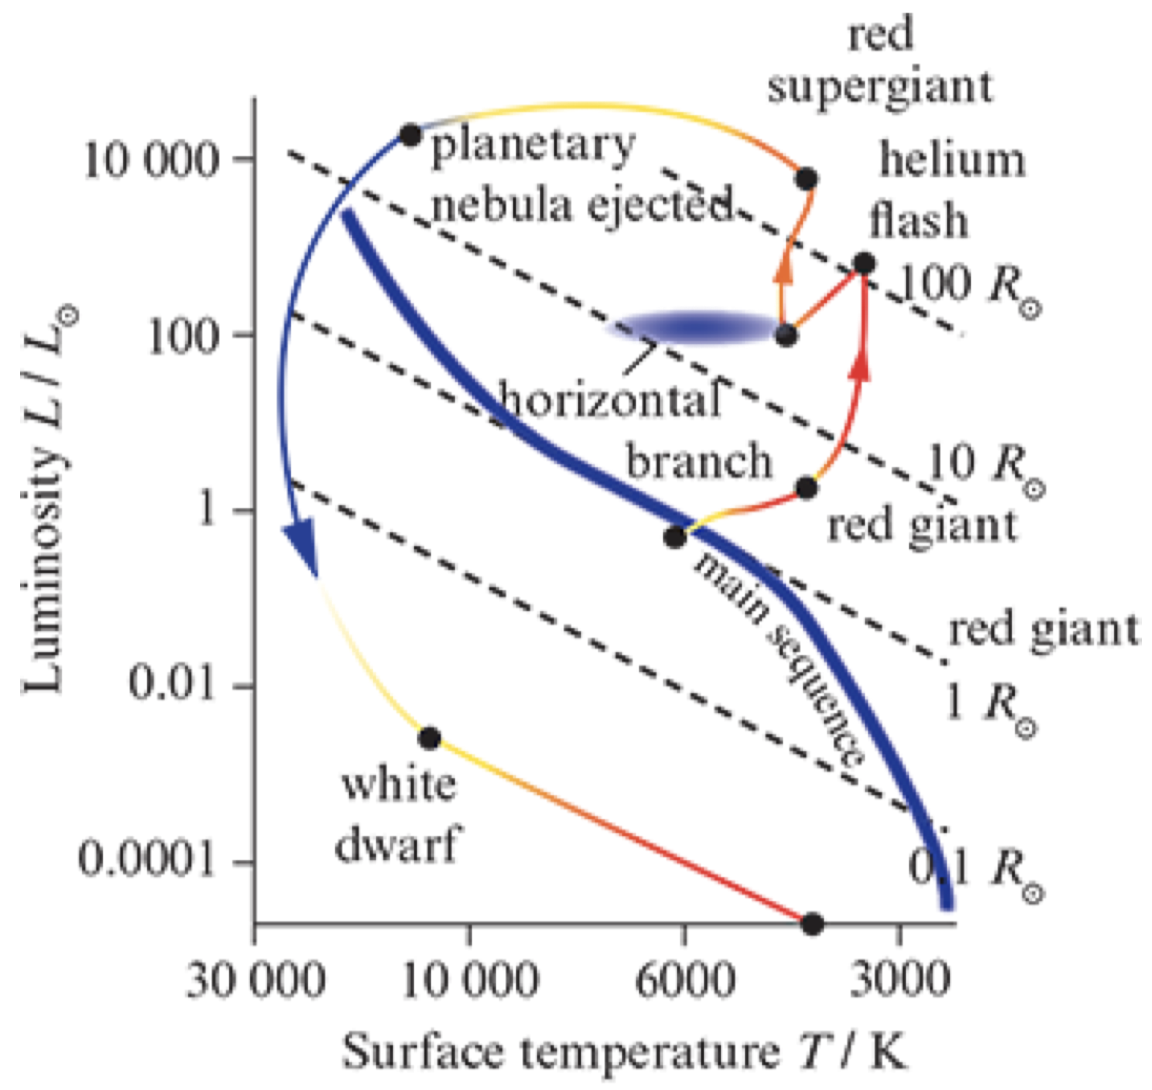
\includegraphics[width=0.3\linewidth]{Screenshot 2026-07-11 at 15.05.05.png}
  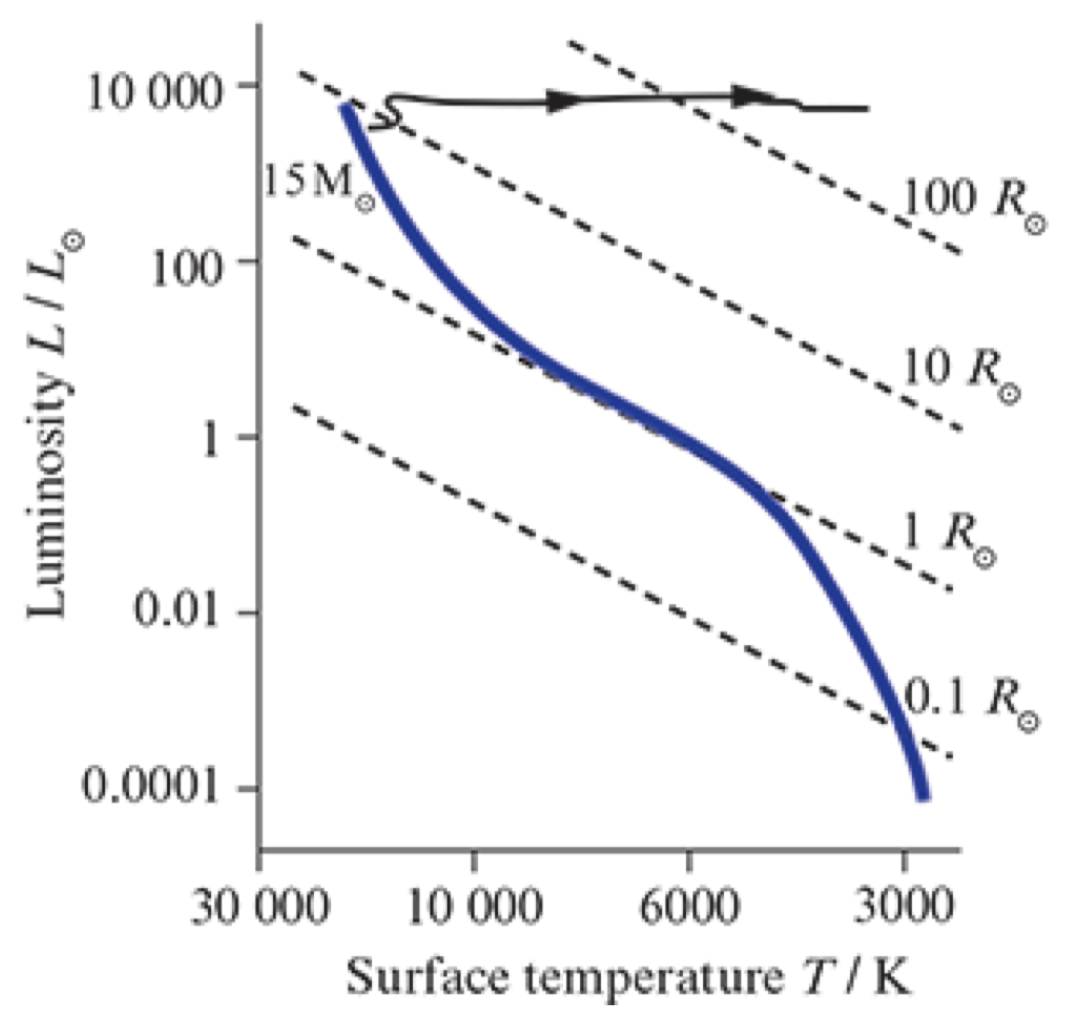
\includegraphics[width=0.3\linewidth]{Screenshot 2026-07-11 at 15.09.57.png}
  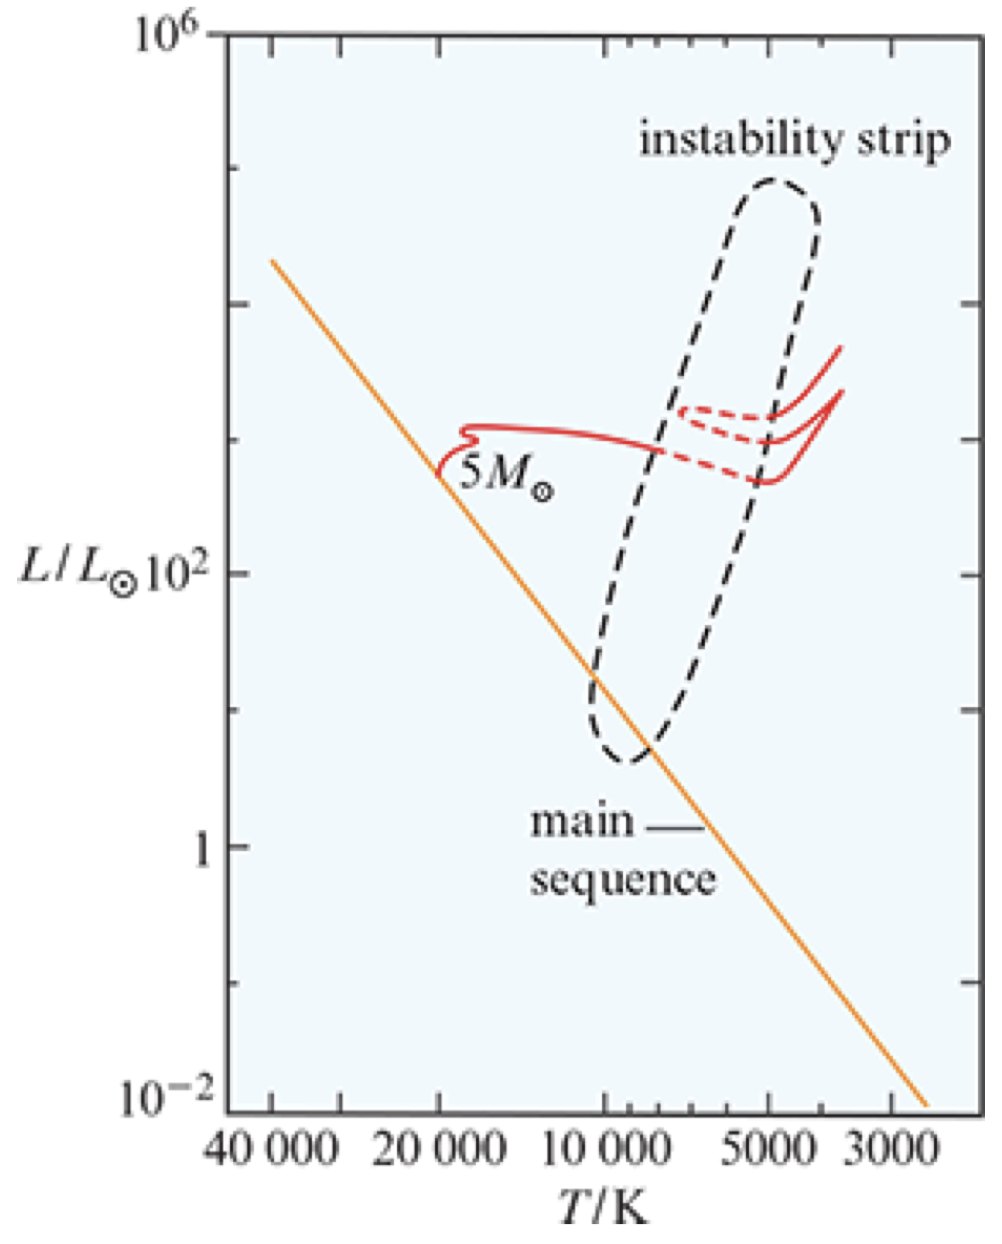
\includegraphics[width=0.225\linewidth]{Screenshot 2026-07-11 at 15.10.19.png}
\end{center}
A star more massive than the sun may go back and forth on the HR diagram several times. The delicate balance between radiation and gravitational pressures has been disturbed; the star tries to find a new equilibrium state but instead the star pulsates, i.e. it grows and then shrinks in size. So the star cools and heats up during these pulsations and that affects the rate and type of nuclear fusion reactions taking place. This makes its luminosity variable, and this is a general characteristic of all stars in the instability region.
\subsubsection*{The Chandrasekhar limit}
It is the largest mass a white dwarf star can have, $1.4M_\odot$.\\
前情提要：
\begin{itemize}
  \item Low mass stars after ejecting mass into space in the planetary nebula explosion leave behind a core.
  \item The conditions in the core mean that the electrons behave as a gas, and the pressure they generate is what keeps the core from collapsing further under its weight. (driven by quantum effect)
  \item The core has now become a white dwarf star. Now exposed, and with no further energy source, the star is doomed to cool down and will then become what is called a black dwarf.
  \item This pressure is able to stop the further collapse of the core only if the mass of the core < the Chandrasekhar limit.
\end{itemize}
\subsubsection*{The Oppenheimer-Volkoff limit}
It is the largest mass a neutron star can have and equals about $3M_\odot$.\\
前情提要：
\begin{itemize}
  \item If the Chandasekhar limit is exceeded, electrons will be forced into protons, turning them into neutrons.
  \item The star is now made almost entirely of neutrons, and it is still contracting rapidly. 
  \item The neutrons get too close to each other, and a pressure develops to prevent them from getting any closer.
  \item But they would still become too close together, and the entire core will now rebound to a larger size.
  \item The rebounding of the core is catastrophic for the star, creating an enormous shockwave travelling outward that tears apart the outer layers of the star. The violent explosion is called the supernova.
  \item The core that is left behind is called a neutron star. The core is kept stable by quantum effects similar to those in the white dwarf if the mass of the core is not more than the Oppenheimer-Volkoff limit. 
\end{itemize}
\subsection{Stellar evolution extension}
\subsubsection*{The creation of elements}
The hydrogen in the universe and most of the helium (and some lithium) were produced at the very earliest times in the life of the universe. The rest of the elements were produced in a process known as nucleosynthesis in stars, in the process of stellar evolution.\\\\
For stars more massive than about 1.5 solar masses there is a second way to fuse hydrogen into helium. This is the CNO (carbon, nitrogen, oxygen) cycle:
\[\begin{aligned}
^1_1\text{H}+^{12}_6\text{C}&\rightarrow ^{13}_7\text{N}+\gamma\\
^{13}_7\text{N}&\rightarrow ^{13}_6\text{C}+^0_1e^++\nu\\
^1_1\text{H}+^{13}_6\text{C}&\rightarrow ^{14}_7\text{N}+\gamma\\
^1_1\text{H}+^{14}_7\text{N}&\rightarrow ^{15}_8\text{O}+\gamma\\
^{15}_8\text{O}&\rightarrow ^{15}_7\text{N}+^0_1e^++\nu\\
^1_1\text{H}+^{15}_7\text{N}&\rightarrow ^{12}_6\text{C}+^4_2\text{He}
\end{aligned}\]
\begin{itemize}
  \item For low mass stars, the helium produced in the p-p chain is collecting in the core of the star surrounded by a thin shell of hydrogen and a bigger hydrogen envelope.
  \item In more massive stars, carbon will replace helium in the core once carbon starts getting produced in the triple alpha process:
  \[
  \begin{aligned}
  ^4_2\text{He}+^4_2\text{He}&\rightarrow ^8_4\text{Be} + \gamma \\
  ^4_2\text{He}+^8_4\text{Be}&\rightarrow ^{12}_6\text{C} + \gamma
  \end{aligned}
  \]
  \begin{itemize}
    \item Only hydrogen in the thin shell is undergoing nuclear fusion. 
    \item The temperature and pressure of helium build up and eventually helium begins to fuse through the triple alpha process, called the "Helium flash".
    \item Carbon collects in the core, with helium now fusing in a thin shell around carbon.
    \item This release of energy blows away the outer layers of the star in an explosion called a planetary nebula; mass is thrown into space leaving behind a helium or carbon core.
  \end{itemize}
\end{itemize}
\begin{center}
  \definecolor{stellarEnvelope}{RGB}{174, 174, 214} % Light periwinkle blue (H Envelope)
\definecolor{stellarHShell}{RGB}{79, 82, 152}    % Deep slate blue (H Shell)
\definecolor{stellarHeShell}{RGB}{177, 214, 171}  % Pastel green (He Core/Shell)
\definecolor{stellarCCore}{RGB}{204, 204, 209}    % Light gray (Carbon Core)
\begin{tikzpicture}[thick, font=\scriptsize,scale=0.7]

  % ==================== DIAGRAM A ====================
  \begin{scope}[xshift=0cm]
    % Outer Hydrogen Envelope
    \draw[fill=stellarEnvelope] (0,0) -- (70:5.5) arc (70:110:5.5) -- cycle;
    
    % Hydrogen Burning Shell
    \draw[fill=stellarHShell] (0,0) -- (70:2.4) arc (70:110:2.4) -- cycle;
    
    % Helium Core
    \draw[fill=stellarHeShell] (0,0) -- (70:1.2) arc (70:110:1.2) -- cycle;
    
    % Labels (placed at the radial midpoint of each layer)
    \node at (90:3.95) {H};
    \node at (90:1.80) {H};
    \node at (90:0.80) {He};
    
  \end{scope}

  % ==================== DIAGRAM B ====================
  \begin{scope}[xshift=6.0cm]
    % Outer Hydrogen Envelope
    \draw[fill=stellarEnvelope] (0,0) -- (70:5.5) arc (70:110:5.5) -- cycle;
    
    % Hydrogen Shell
    \draw[fill=stellarHShell] (0,0) -- (70:2.8) arc (70:110:2.8) -- cycle;
    
    % Helium Shell
    \draw[fill=stellarHeShell] (0,0) -- (70:1.9) arc (70:110:1.9) -- cycle;
    
    % Carbon Core
    \draw[fill=stellarCCore] (0,0) -- (70:1.0) arc (70:110:1.0) -- cycle;
    
    % Labels (placed at the radial midpoint of each layer)
    \node at (90:4.15) {H};
    \node at (90:2.35) {H};
    \node at (90:1.45) {He};
    \node at (90:0.70) {C};
    
  \end{scope}

\end{tikzpicture}
\end{center}
For stars with different sizes of mass:
\begin{itemize}
  \item $M<0.25M_\odot$: white dwarf with Helium core:
  \[4^1_1\text{H}\rightarrow ^4_2\text{He}+2^0_1e^++2\nu +2\gamma\]
  \item $0.25M_\odot<M<8M_\odot$: white dwarf with Carbon core (triple alpha process just mentioned)
  \item $8M_\odot<M<12M_\odot$: white dwarf with Oxygen / Neon / Magnesium core:
  \[
  \begin{aligned}
    ^4_2\text{He}+^{12}_6\text{C}&\rightarrow ^{16}_8\text{O}+\gamma\\
    ^{12}_6\text{C}+^{12}_6\text{C}&\rightarrow ^{20}_{10}\text{Ne}+^4_2\text{He}\\
    ^{12}_6\text{C}+^{12}_6\text{C}&\rightarrow ^{23}_{11}\text{Na}+^2_1\text{H}\\
    ^{12}_6\text{C}+^{12}_6\text{C}&\rightarrow ^{23}_{12}\text{Mg}+^1_0n\\
    ^{16}_8\text{O}+^{16}_8\text{O}&\rightarrow^{28}_{14}\text{Si}+^4_2\text{He}
  \end{aligned}
  \]
  \item $12M_\odot<M<40M_\odot$: Neutron star
  \item $M>40M_\odot$: Black hole
\end{itemize}
Fusion cannot produce elements heavier than iron, since the binding energy per nucleon peaks near iron and further fusion is not energetically possible. 
Elements heavier than iron are produced during supernova explosions through neutron absorption.
\begin{center}
  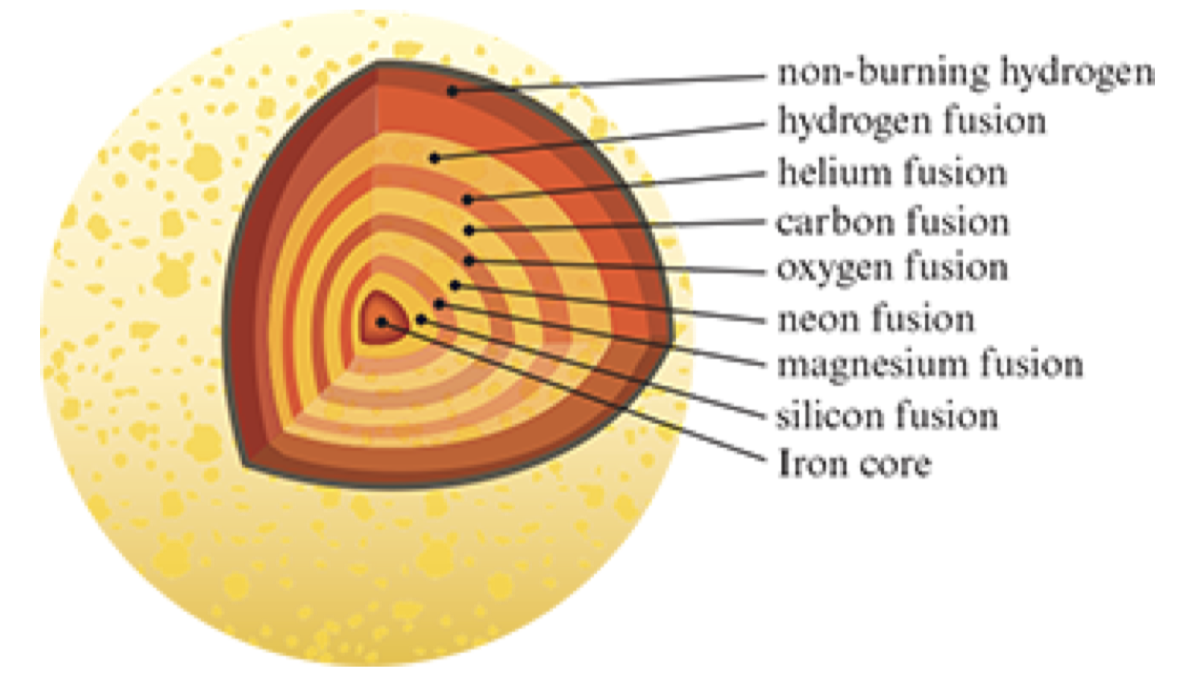
\includegraphics[width=0.4\linewidth]{Screenshot 2026-07-11 at 18.50.16.png}
\end{center}
\newpage
\unnumberedsection{Appendices}
\appendix
A versatile method for doing physics questions, the GUESS method:
\begin{itemize}
\item G: given information
\item U: unknown information
\item E: equation to connect the given and unknown info
\item S: substitute
\item S: solve problem
\end{itemize}
% =====================================================================
% APPENDIX A — COMMON CONSTANTS
% =====================================================================
\section{Common constants}
\renewcommand{\arraystretch}{1.4}
\begin{longtable}{@{} M{1.8cm} l L{9cm} @{}}
\toprule
\textbf{Symbol} & \textbf{Value} & \textbf{Name \& significance / usage} \\
\midrule
\endfirsthead
\multicolumn{3}{c}{{\tablename\ \thetable{} -- continued}} \\
\toprule
\textbf{Symbol} & \textbf{Value} & \textbf{Name \& significance / usage} \\
\midrule
\endhead
\midrule
\multicolumn{3}{r}{{Continued on next page\ldots}} \\
\endfoot
\bottomrule
\endlastfoot
% --- Fundamental constants ---
c & $3.00\times10^{8}\ \text{m\,s}^{-1}$ & Speed of light in vacuum; maximum speed limit, central to relativity and $E=mc^2$. \\
h & $6.63\times10^{-34}\ \text{J\,s}$ & Planck constant; relates photon energy to frequency ($E=hf$) and appears in de Broglie wavelength. \\
e & $1.60\times10^{-19}\ \text{C}$ & Elementary charge; basic quantum unit of charge (proton charge, electron charge magnitude). \\
G & $6.67\times10^{-11}\ \text{N\,m}^{2}\,\text{kg}^{-2}$ & Gravitational constant; proportionality constant in Newton's law of gravitation. \\
g & $9.8\ \text{m\,s}^{-2}$ & Acceleration of free fall at Earth's surface (directed downward). \\
k & $8.99\times10^{9}\ \text{N\,m}^{2}\,\text{C}^{-2}$ & Coulomb constant; $k=\dfrac{1}{4\pi\varepsilon_0}$, proportionality constant in Coulomb's law. \\
\varepsilon_0 & $8.85\times10^{-12}\ \text{C}^{2}\,\text{N}^{-1}\,\text{m}^{-2}$ & Permittivity of free space; relates electric field to charge in vacuum. \\
\mu_0 & $4\pi\times10^{-7}\ \text{T\,m\,A}^{-1}$ & Magnetic permeability of free space; relates magnetic field to current. \\
k_B & $1.38\times10^{-23}\ \text{J\,K}^{-1}$ & Boltzmann constant; relates average molecular kinetic energy to temperature ($k_B=R/N_A$). \\
N_A & $6.02\times10^{23}\ \text{mol}^{-1}$ & Avogadro constant; number of particles per mole of substance. \\
R & $8.31\ \text{J\,mol}^{-1}\,\text{K}^{-1}$ & Molar gas constant; universal constant in the ideal gas law $PV=nRT$. \\
\sigma & $5.67\times10^{-8}\ \text{W\,m}^{-2}\,\text{K}^{-4}$ & Stefan--Boltzmann constant; proportionality constant in $P=\sigma AT^4$. \\
b & $2.90\times10^{-3}\ \text{K\,m}$ & Wien's displacement constant; links peak wavelength of black-body spectrum to temperature. \\
u & $1.66\times10^{-27}\ \text{kg}$ & Atomic mass unit; $\tfrac{1}{12}$ mass of carbon-12, standard nuclear mass unit. \\
uc^2 & $931.5\ \text{MeV}$ & Energy equivalent of 1 atomic mass unit ($uc^2$); used in nuclear mass--energy calculations. \\
m_e & $9.11\times10^{-31}\ \text{kg}$ & Electron rest mass; mass of the electron (beta particle). \\
m_p & $1.67\times10^{-27}\ \text{kg}$ & Proton rest mass; mass of a proton (hydrogen nucleus). \\
m_n & $1.675\times10^{-27}\ \text{kg}$ & Neutron rest mass; mass of a free neutron. \\
a_0 & $5.29\times10^{-11}\ \text{m}$ & Bohr radius; smallest allowed orbital radius of the hydrogen electron. \\
R_0 & $1.2\times10^{-15}\ \text{m}$ & Nuclear radius constant; characteristic length scale in $R=R_0A^{1/3}$. \\
h/(m_ec) & $2.43\times10^{-12}\ \text{m}$ & Compton wavelength of the electron; characteristic wavelength-shift scale in Compton scattering. \\
\gamma_\text{mono} & 5/3 & Adiabatic index for a monatomic ideal gas; ratio of specific heats. \\
\midrule
\multicolumn{3}{l}{\textit{Astronomical \& planetary data}} \\
\midrule
S & $\approx 1400\ \text{W\,m}^{-2}$ & Solar constant; solar intensity at the top of Earth's atmosphere. \\
L_\odot & $3.9\times10^{26}\ \text{W}$ & Sun's luminosity; total radiated power of the Sun. \\
R_\odot & $7.0\times10^{8}\ \text{m}$ & Sun's radius; used in stellar surface intensity calculations. \\
d_\text{au} & $1.5\times10^{11}\ \text{m}$ & Astronomical unit (Earth--Sun distance); used in solar constant and parallax. \\
\alpha_\text{Earth} & $\approx 0.30$ & Earth's average albedo; fraction of incident solar radiation reflected. \\
1\ \text{atm} & $1.01\times10^{5}\ \text{Pa}$ & Standard atmospheric pressure at sea level. \\
1\ \text{pc} & $3.09\times10^{16}\ \text{m}=3.27\ \text{ly}$ & Parsec; distance at which 1\,AU subtends 1 arcsecond. \\
\end{longtable}

\newpage
% =====================================================================
% APPENDIX B — FORMULA LIST (BY UNIT)
% =====================================================================
\section{Formula list}
\renewcommand{\arraystretch}{1.5}

\subsection{Unit A — Space, time and motion}

\begin{longtable}{@{} L{2.2cm} M{6cm} L{7.5cm} @{}}
\toprule
\textbf{Topic} & \textbf{Formula} & \textbf{Significance / usage} \\
\midrule
\endfirsthead
\multicolumn{3}{c}{{\tablename\ \thetable{} -- continued}} \\
\toprule
\textbf{Topic} & \textbf{Formula} & \textbf{Significance / usage} \\
\midrule
\endhead
\midrule
\multicolumn{3}{r}{{Continued on next page\ldots}} \\
\endfoot
\bottomrule
\endlastfoot
Kinematics & v=\dfrac{\Delta s}{\Delta t} & Average speed (total distance over total time). \\
Kinematics & s=s_i+vt & Position for uniform motion with initial position. \\
Kinematics & v=u+at & Velocity as a function of time (constant acceleration). \\
Kinematics & s=ut+\dfrac{1}{2}at^2 & Displacement as a function of time. \\
Kinematics & v^2=u^2+2as & Velocity--displacement relationship (no time). \\
Kinematics & s=\dfrac{u+v}{2}\,t & Displacement from average velocity. \\
Kinematics & v=\dfrac{ds}{dt},\quad a=\dfrac{dv}{dt}=\dfrac{d^2s}{dt^2} & Calculus definitions of velocity and acceleration. \\
Projectile & V_x=u\cos\theta,\quad V_y=u\sin\theta-gt & Horizontal and vertical velocity components. \\
Projectile & x=ut\cos\theta,\quad y=ut\sin\theta-\tfrac{1}{2}gt^2 & Horizontal and vertical position vs.\ time. \\
Projectile & y_\text{max}=\dfrac{u^2\sin^2\theta}{2g} & Maximum height of a projectile. \\
Projectile & R=\dfrac{u^2\sin 2\theta}{g} & Range (maximum horizontal displacement). \\
Projectile & t_\text{flight}=\dfrac{2u\sin\theta}{g} & Total time of flight (level ground). \\
Drag & F=kv\;\text{(low }v\text{)},\quad F=kv^2\;\text{(high }v\text{)} & Fluid resistance force. \\
Drag & v_T=\dfrac{mg}{k} & Terminal speed (net force $=0$). \\
Forces & W=mg & Weight of a body. \\
Forces & F=kx & Hooke's law for a spring (extension $x$). \\
Forces & F_D=6\pi\eta rv & Stokes' law drag on a sphere. \\
Forces & F_B=\rho gV_\text{imm} & Buoyant force (upthrust). \\
Forces & f_d=\mu_dR,\quad f_s=\mu_sR & Dynamic and maximum static friction. \\
Newton's 2nd law & F=ma & Net force equals mass times acceleration. \\
Newton's 2nd law & F=\dfrac{\Delta p}{\Delta t} & Newton's second law in momentum form. \\
Inclined plane & R=mg\cos\theta,\quad f=mg\sin\theta & Normal force and friction on an incline. \\
Inclined plane & \mu_s=\tan\theta_\text{max} & Coefficient of static friction from equilibrium angle. \\
Circular motion & v=r\omega=\dfrac{2\pi r}{T} & Linear speed in circular motion. \\
Circular motion & \omega=\dfrac{2\pi}{T}=2\pi f & Angular speed for a full revolution. \\
Circular motion & a_c=\dfrac{v^2}{r}=\omega^2r & Centripetal acceleration (toward centre). \\
Energy & W=Fs\cos\theta & Work done by a constant force. \\
Energy & E_k=\dfrac{1}{2}mv^2 & Kinetic energy. \\
Energy & E_p=mg\Delta h & Gravitational potential energy. \\
Energy & E_H=\dfrac{1}{2}kx^2 & Elastic potential energy of a spring. \\
Energy & W_\text{net}=\Delta E_k & Work--kinetic energy theorem. \\
Energy & E_T=E_k+E_p & Conservation of total mechanical energy. \\
Power & P=\dfrac{W}{t}=Fv & Power (rate of work; force $\times$ speed). \\
Power & \eta=\dfrac{E_\text{out}}{E_\text{in}} & Efficiency. \\
Momentum & p=mv & Linear momentum. \\
Momentum & J=\Delta p=F\,\Delta t & Impulse (area under $F$--$t$ graph). \\
Momentum & \sum p_\text{before}=\sum p_\text{after} & Conservation of momentum. \\
Momentum & E_k=\dfrac{p^2}{2m} & Kinetic energy in terms of momentum. \\
Momentum & M\dfrac{dv}{dt}=u\dfrac{dm}{dt} & Rocket equation ($u$ = exhaust speed). \\
Rotation & \omega=\omega_1+\alpha t & Rotational kinematics (velocity--time). \\
Rotation & \theta=\omega_1t+\tfrac{1}{2}\alpha t^2 & Rotational kinematics (displacement--time). \\
Rotation & \omega^2=\omega_1^2+2\alpha\theta & Rotational kinematics (velocity--displacement). \\
Rotation & \tau=Fr\sin\theta & Torque (force $\times$ perpendicular distance). \\
Rotation & I=\sum m_ir_i^2 & Moment of inertia definition. \\
Rotation & \tau_\text{net}=I\alpha & Newton's second law for rotation. \\
Rotation & E_k=\dfrac{1}{2}I\omega^2 & Rotational kinetic energy. \\
Rotation & L=I\omega & Angular momentum. \\
Rotation & P=\tau\omega & Rotational power. \\
Rotation & u=\omega R & Rolling-without-slipping condition. \\
Rotation & E_k=\dfrac{1}{2}Mv^2+\dfrac{1}{2}I\omega^2 & Total KE of a rolling body. \\
Rotation & a=\dfrac{g\sin\theta}{1+I/(MR^2)} & Linear acceleration of a body rolling down an incline. \\
Mom.\ of inertia & I=MR^2\;\text{(ring)} & Moment of inertia of a ring. \\
Mom.\ of inertia & I=\tfrac{1}{2}MR^2 & Moment of inertia of a disk / cylinder. \\
Mom.\ of inertia & I=\tfrac{2}{5}MR^2 & Moment of inertia of a sphere. \\
Mom.\ of inertia & I=\tfrac{1}{12}ML^2 & Moment of inertia of a rod. \\
Relativity & \gamma=\dfrac{1}{\sqrt{1-v^2/c^2}} & Lorentz factor. \\
Relativity & x'=\gamma(x-vt),\quad t'=\gamma\!\left(t-\dfrac{v}{c^2}x\right) & Lorentz position and time transformations. \\
Relativity & \Delta t=\gamma\,\Delta t' & Time dilation ($\Delta t'$ = proper time). \\
Relativity & L=\dfrac{L_0}{\gamma} & Length contraction ($L_0$ = proper length). \\
Relativity & u=\dfrac{u'+v}{1+u'v/c^2} & Relativistic velocity addition. \\
Relativity & (c\Delta t)^2-(\Delta x)^2=\text{invariant} & Invariant spacetime interval (all observers agree). \\
\end{longtable}

\newpage
\subsection{Unit B — The particulate nature of matter}

\begin{longtable}{@{} L{2.2cm} M{6cm} L{7.5cm} @{}}
\toprule
\textbf{Topic} & \textbf{Formula} & \textbf{Significance / usage} \\
\midrule
\endfirsthead
\multicolumn{3}{c}{{\tablename\ \thetable{} -- continued}} \\
\toprule
\textbf{Topic} & \textbf{Formula} & \textbf{Significance / usage} \\
\midrule
\endhead
\midrule
\multicolumn{3}{r}{{Continued on next page\ldots}} \\
\endfoot
\bottomrule
\endlastfoot
Thermal & \rho=\dfrac{m}{V} & Density (mass per unit volume). \\
Thermal & \overline{E}_k=\dfrac{3}{2}k_BT & Average random kinetic energy of a molecule. \\
Thermal & T(\text{K})=T(^\circ\text{C})+273 & Celsius to kelvin conversion. \\
Thermal & Q=mc\Delta T & Heat to change temperature (specific heat capacity $c$). \\
Thermal & Q=mL & Latent heat for phase change ($L=L_F$ fusion, $L_V$ vaporisation). \\
Thermal & \dfrac{\Delta T}{\Delta t}=k(T-T_s) & Newton's law of cooling. \\
Thermal & \dfrac{\Delta Q}{\Delta t}=kA\dfrac{\Delta T}{\Delta x} & Rate of heat conduction. \\
Radiation & P=\sigma AT^4 & Stefan--Boltzmann law (total black-body power). \\
Radiation & \lambda_\text{max}T=2.90\times10^{-3}\ \text{m\,K} & Wien's displacement law. \\
Radiation & P=e\sigma AT^4 & Modified Stefan--Boltzmann for real bodies (emissivity $e$). \\
Radiation & I=\dfrac{P}{4\pi d^2} & Intensity at distance $d$ from an isotropic source. \\
Radiation & e+\alpha=1 & Emissivity--albedo relation. \\
Radiation & (1-\alpha)\dfrac{S}{4}=\sigma T^4 & Earth's radiative energy balance (no greenhouse). \\
Gas laws & PV=nRT=k_BNT & Ideal gas law (equation of state). \\
Gas laws & \dfrac{P_1V_1}{T_1}=\dfrac{P_2V_2}{T_2} & Combined gas law (fixed $n$). \\
Gas laws & P=\dfrac{1}{3}\rho c^2 & Kinetic theory pressure (rms speed $c$). \\
Gas laws & \overline{E}_k=\dfrac{1}{2}mc^2=\dfrac{3}{2}k_BT & Average molecular KE from rms speed / temperature. \\
Gas laws & U=\dfrac{3}{2}Nk_BT=\dfrac{3}{2}nRT & Internal energy of a monatomic ideal gas. \\
Thermo & \Delta U=Q-W & First law ($W$ = work done \emph{by} gas). \\
Thermo & W=P\Delta V & Work done during volume change at constant pressure. \\
Thermo & \Delta S=\dfrac{Q}{T} & Entropy change for reversible heat transfer. \\
Thermo & S=k_B\ln\Omega & Statistical definition of entropy (microstates $\Omega$). \\
Thermo & \eta=1-\dfrac{T_C}{T_H} & Carnot (maximum) efficiency of a heat engine. \\
Thermo & P_1V_1^\gamma=P_2V_2^\gamma & Adiabatic process relation ($\gamma=5/3$ for monatomic). \\
Circuits & V=\dfrac{W}{q} & Potential difference (work per unit charge). \\
Circuits & I=\dfrac{\Delta q}{\Delta t} & Electric current (rate of flow of charge). \\
Circuits & R=\dfrac{V}{I} & Ohm's law / definition of resistance. \\
Circuits & R=\rho\dfrac{L}{A} & Resistance from resistivity, length, area. \\
Circuits & P=IV=I^2R=\dfrac{V^2}{R} & Electric power (multiple forms). \\
Circuits & \varepsilon=\dfrac{W}{q}=\dfrac{P}{I} & Electromotive force (e.m.f.). \\
Circuits & R_T=R_1+R_2+\cdots & Resistors in series. \\
Circuits & \dfrac{1}{R_T}=\dfrac{1}{R_1}+\dfrac{1}{R_2}+\cdots & Resistors in parallel. \\
\end{longtable}

\newpage
\subsection{Unit C — Wave behaviour}

\begin{longtable}{@{} L{2.2cm} M{6cm} L{7.5cm} @{}}
\toprule
\textbf{Topic} & \textbf{Formula} & \textbf{Significance / usage} \\
\midrule
\endfirsthead
\multicolumn{3}{c}{{\tablename\ \thetable{} -- continued}} \\
\toprule
\textbf{Topic} & \textbf{Formula} & \textbf{Significance / usage} \\
\midrule
\endhead
\midrule
\multicolumn{3}{r}{{Continued on next page\ldots}} \\
\endfoot
\bottomrule
\endlastfoot
SHM & a=-\omega^2x & Defining condition of SHM (acceleration $\propto$ displacement). \\
SHM & x=x_0\sin(\omega t+\phi) & Displacement as a function of time. \\
SHM & \omega=\sqrt{\dfrac{k}{m}},\quad T=2\pi\sqrt{\dfrac{m}{k}} & Angular frequency and period of a mass--spring system. \\
SHM & T=2\pi\sqrt{\dfrac{L}{g}} & Period of a simple pendulum. \\
SHM & v_\text{max}=\omega x_0,\quad a_\text{max}=\omega^2x_0 & Maximum velocity and acceleration in SHM. \\
SHM & E_T=\dfrac{1}{2}m\omega^2x_0^2 & Total energy of an SHM system. \\
SHM & E_k=\tfrac{1}{2}m\omega^2(x_0^2-x^2),\quad E_p=\tfrac{1}{2}m\omega^2x^2 & KE and PE at displacement $x$. \\
SHM & v=\pm\omega\sqrt{x_0^2-x^2} & Velocity as a function of displacement. \\
Waves & v=f\lambda & Wave speed (frequency $\times$ wavelength). \\
Waves & \Delta\phi=2\pi\dfrac{\Delta x}{\lambda} & Phase difference between two points on a wave. \\
Waves & I\propto A^2 & Intensity proportional to amplitude squared. \\
Refraction & n_1\sin\theta_1=n_2\sin\theta_2 & Snell's law of refraction. \\
Refraction & n=\dfrac{c_\text{vacuum}}{c_\text{medium}} & Definition of refractive index. \\
Refraction & \sin\theta_c=\dfrac{1}{n} & Critical angle for total internal reflection. \\
Interference & |S_1P-S_2P|=n\lambda & Path difference for constructive interference. \\
Interference & |S_1P-S_2P|=(n+\tfrac{1}{2})\lambda & Path difference for destructive interference. \\
Interference & s=\dfrac{\lambda D}{d} & Fringe spacing in Young's double-slit experiment. \\
Diffraction & b\sin\theta=\lambda & First minimum of single-slit diffraction (slit width $b$). \\
Diffraction & d\sin\theta=n\lambda & Diffraction-grating equation for the $n$th-order maximum. \\
Diffraction & I_\text{central}=N^2I_\text{single} & Central-maximum intensity with $N$ slits. \\
Standing waves & \lambda_n=\dfrac{2L}{n},\quad f_n=n\dfrac{v}{2L} & Harmonics on a string fixed at both ends. \\
Standing waves & \lambda_n=\dfrac{4L}{n}\;(n\text{ odd}) & Allowed wavelengths in a pipe closed at one end. \\
Doppler & f'=f\!\left(\dfrac{v}{v\pm u_s}\right) & Observed frequency for a moving source. \\
Doppler & f'=f\!\left(\dfrac{v\pm u_o}{v}\right) & Observed frequency for a moving observer. \\
Doppler & \dfrac{\Delta f}{f}\approx\dfrac{v}{c} & Approximate Doppler shift for light ($v\ll c$). \\
\end{longtable}

\newpage
\subsection{Unit D — Fields}

\begin{longtable}{@{} L{2.2cm} M{6cm} L{7.5cm} @{}}
\toprule
\textbf{Topic} & \textbf{Formula} & \textbf{Significance / usage} \\
\midrule
\endfirsthead
\multicolumn{3}{c}{{\tablename\ \thetable{} -- continued}} \\
\toprule
\textbf{Topic} & \textbf{Formula} & \textbf{Significance / usage} \\
\midrule
\endhead
\midrule
\multicolumn{3}{r}{{Continued on next page\ldots}} \\
\endfoot
\bottomrule
\endlastfoot
Gravitation & F=\dfrac{GMm}{r^2} & Newton's law of gravitation (force between two masses). \\
Gravitation & g=\dfrac{GM}{r^2} & Gravitational field strength at distance $r$ from mass $M$. \\
Gravitation & V_g=-\dfrac{GM}{r} & Gravitational potential (zero at infinity). \\
Gravitation & E_p=mV_g=-\dfrac{GMm}{r} & Gravitational potential energy of two masses. \\
Gravitation & g=-\dfrac{dV_g}{dr} & Field strength as the negative potential gradient. \\
Gravitation & v_\text{orb}=\sqrt{\dfrac{GM}{r}} & Orbital speed of a satellite in circular orbit. \\
Gravitation & T^2=\dfrac{4\pi^2r^3}{GM} & Kepler's third law (period squared vs.\ radius cubed). \\
Gravitation & v_\text{esc}=\sqrt{\dfrac{2GM}{r}} & Escape speed from distance $r$. \\
Gravitation & E_T=-\dfrac{GMm}{2r} & Total energy of a body in circular orbit. \\
Electric & F=\dfrac{kQq}{r^2} & Coulomb's law (force between two charges). \\
Electric & E=\dfrac{F}{q}=\dfrac{kQ}{r^2} & Electric field strength from a point charge. \\
Electric & V_e=\dfrac{kQ}{r} & Electric potential at distance $r$ from a point charge. \\
Electric & E_p=qV_e=\dfrac{kQq}{r} & Electric potential energy of two charges. \\
Electric & E=-\dfrac{dV_e}{dr} & Electric field as the negative potential gradient. \\
Electric & E=\dfrac{V}{d} & Uniform field between parallel plates. \\
Magnetic & F=qvB\sin\theta & Magnetic force on a moving charge. \\
Magnetic & F=BIL\sin\theta & Magnetic force on a current-carrying wire. \\
Magnetic & B=\dfrac{\mu_0I}{2\pi r} & Field at distance $r$ from a long straight wire. \\
Magnetic & \dfrac{F}{L}=\dfrac{\mu_0I_1I_2}{2\pi r} & Force per unit length between two parallel wires. \\
Motion in $E$ & a=\dfrac{qE}{m},\quad y=\dfrac{qE}{2m}t^2 & Acceleration and deflection of a charge in a uniform field. \\
Motion in $B$ & R=\dfrac{mv}{qB} & Radius of circular motion of a charge in a magnetic field. \\
Motion in $B$ & T=\dfrac{2\pi m}{qB} & Period of circular motion in a magnetic field. \\
Velocity selector & E=vB & Condition for undeflected motion in crossed $E$ and $B$ fields. \\
Induction & \varepsilon=BLv & Motional e.m.f.\ in a conductor moving through a field. \\
Induction & \Phi=BA\cos\theta & Magnetic flux through a loop. \\
Induction & \Phi_\text{link}=NBA\cos\theta & Magnetic flux linkage for a coil of $N$ turns. \\
Induction & \varepsilon=-N\dfrac{d\Phi}{dt} & Faraday's law of electromagnetic induction. \\
AC generator & V=V_\text{max}\sin(2\pi ft),\quad V_\text{max}=2\pi fNBA & Induced e.m.f.\ in a rotating coil. \\
\end{longtable}

\newpage
\subsection{Unit E — Nuclear and quantum physics}

\begin{longtable}{@{} L{2.2cm} M{6cm} L{7.5cm} @{}}
\toprule
\textbf{Topic} & \textbf{Formula} & \textbf{Significance / usage} \\
\midrule
\endfirsthead
\multicolumn{3}{c}{{\tablename\ \thetable{} -- continued}} \\
\toprule
\textbf{Topic} & \textbf{Formula} & \textbf{Significance / usage} \\
\midrule
\endhead
\midrule
\multicolumn{3}{r}{{Continued on next page\ldots}} \\
\endfoot
\bottomrule
\endlastfoot
Atomic & E_n=-\dfrac{13.6}{n^2}\ \text{eV} & Energy levels of the hydrogen atom. \\
Atomic & mvr=n\dfrac{h}{2\pi} & Bohr quantisation of angular momentum. \\
Atomic & r_n=a_0n^2 & Allowed orbital radii of the electron. \\
Quantum & E=hf=\dfrac{hc}{\lambda} & Photon energy. \\
Quantum & p=\dfrac{h}{\lambda} & Photon momentum (and de Broglie relation). \\
Quantum & E_k=hf-\phi & Einstein's photoelectric equation ($\phi$ = work function). \\
Quantum & eV_s=E_{k,\text{max}} & Maximum photoelectron KE from stopping voltage. \\
Quantum & \lambda' - \lambda=\dfrac{h}{m_ec}(1-\cos\theta) & Compton scattering wavelength shift. \\
Quantum & \lambda=\dfrac{h}{p}=\dfrac{h}{\sqrt{2mqV}} & de Broglie wavelength of a particle. \\
Quantum & 2d\sin\theta=n\lambda & Bragg / Davisson--Germer diffraction condition. \\
Nuclear & N=A-Z & Number of neutrons ($A$ = mass no., $Z$ = atomic no.). \\
Nuclear & R=R_0A^{1/3} & Nuclear radius from mass number. \\
Nuclear & \mu=Zm_p+Nm_n-M_\text{nucleus} & Mass defect. \\
Nuclear & E_b=\mu c^2 & Binding energy. \\
Nuclear & E=mc^2 & Einstein mass--energy equivalence. \\
Nuclear & b=\dfrac{E_b}{A} & Binding energy per nucleon (stability measure). \\
Nuclear & \dfrac{dN}{dt}=-\lambda N & Differential radioactive decay law. \\
Nuclear & N=N_0e^{-\lambda t} & Exponential decay of number of nuclei. \\
Nuclear & A=\lambda N & Activity (decays per second). \\
Nuclear & \lambda T_{1/2}=\ln 2 & Relation between decay constant and half-life. \\
Nuclear & Q=\sum n(b_\text{products}-b_\text{reactants}) & Energy released in a nuclear reaction. \\
Stars & R=\sqrt{\dfrac{L}{4\pi\sigma T^4}} & Stellar radius from luminosity and surface temperature. \\
Stars & d(\text{pc})=\dfrac{1}{p(\text{arcsec})} & Parallax distance in parsecs. \\
\end{longtable}
\end{document}
